\documentclass[a4paper,12pt]{report}
\usepackage[margin=0.5in]{geometry}
\usepackage{hyperref}
\usepackage{setspace}
\usepackage{lastpage}
\usepackage{tabularx}

\usepackage[nottoc,numbib]{tocbibind}
  % Preamble packages:
\usepackage{booktabs}
\usepackage{multirow}
\usepackage{caption}
\usepackage{multicol}
\usepackage{caption}



% for apa with apa
% \usepackage{natbib} 
% for ieee with IEEEtran
\usepackage[numbers]{natbib}
\usepackage{float}
\usepackage{grffile}  % Add to preamble
\usepackage{titlesec} % Add this line for chapter formatting

\usepackage{graphicx}

\usepackage{float} % If you use [H] placement


% Required in preamble
\usepackage{pgfplots}      % Core plotting package
\pgfplotsset{compat=1.18} % Set compatibility mode (use newest version available) % For general graphics handling (usually auto-loaded)

% Required packages in preamble
\usepackage{algorithm}      % For algorithm float environment
\usepackage{algpseudocode}  % For algorithmic structure (functions, loops, etc.)
\usepackage{xspace}         % For smart spacing after macros (optional but recommended)

\usepackage{csquotes}

\renewcommand{\familydefault}{\sfdefault}
\usepackage{helvet}
\usepackage{amsmath}
\usepackage{tikz}
\usetikzlibrary{positioning}

\renewcommand{\contentsname}{Table of Contents}


\usepackage{booktabs} % For professional quality tables
\usepackage{caption}  % For captions of figures and tables
\usepackage{subcaption} % For subfigures within a figure environment
% \usepackage[backend=biber, style=apa]{biblatex} % Example for bibliography (if needed, adapt style)
% \addbibresource{references.bib} % Link to your bibliography file
% \usepackage{hyperref} % Optional: for clickable links and references
% \usepackage[capitalise]{cleveref} % Optional: for smart cross-referencing (e.g., Figure 1, Table 2)

\newenvironment{smallquote}
  {\begin{quote}\footnotesize\vspace{0em}}
  {\vspace{0em}\end{quote}}


\usepackage{pgffor}
% MAKE Smaller
% make lists small
\usepackage{enumitem}
\setlist{nosep} % Removes extra space in itemize/enumerate

\titlespacing*{\section}{0pt}{0.5em}{0.5em}
\titlespacing*{\subsection}{0pt}{0.5em}{0.5em}

% % \titleformat{\section}
% %   {\normalfont\normalsize\bfseries}
% %   {\thesection}{1em}{}

% \titleformat{\subsection}
%   {\normalfont\small\bfseries}
%   {\thesubsection}{1em}{}

\setlength{\parindent}{1.5em}
\setlength{\parskip}{0.5em} % Adjust spacing between paragraphs

% Customise hyperlink appearance (Optional)
\hypersetup{
    colorlinks=true,        % Enable colored links
    linkcolor=black,        % Color for internal links (TOC, sections, etc.)
    citecolor=black,        % Color for citation links
    filecolor=black,        % Color for file links
    urlcolor=blue          % Color for external URLs
}

% \titleformat{\chapter}[hang]{\normalfont\huge\bfseries}{\thechapter.}{0.5em}{}
% \titleformat{\chapter}[display]
%   {\normalfont\Large\bfseries}
%   {}
%   {0pt}
%   {\vspace{-2em}}
% \titlespacing*{\chapter}{0pt}{-2em}{1em}

% % Chapter title (smaller than default)
% \titleformat{\chapter}[display]
%   {\normalfont\Large\bfseries}
%   {} % No label
%   {0pt}
%   {\vspace{-2em}}

% % Section title (even smaller)
% \titleformat{\section}
%   {\normalfont\small\bfseries}
%   {\thesection}{1em}{}

% \titleformat{\chapter}[display]
%   {\normalfont\LARGE\bfseries}
%   {\thechapter}{1em}{} % <- this line sets the number before the title
% \titlespacing*{\chapter}{0pt}{-2em}{1em}

% \usepackage{titlesec}

\titleformat{\chapter}[block] % or [hang]
  {\normalfont\LARGE\bfseries}
  {\thechapter}{1em}{}

\titlespacing*{\chapter}{0pt}{-2em}{1em}


% Section: Large and bold
\titleformat{\section}
  {\normalfont\Large\bfseries}
  {\thesection}{1em}{}
\titlespacing*{\section}{0pt}{0.5em}{0.5em}

% Subsection: Slightly smaller than section, bold
\titleformat{\subsection}
  {\normalfont\large\bfseries}
  {\thesubsection}{1em}{}
\titlespacing*{\subsection}{0pt}{0.4em}{0.4em}

% Subsubsection: Normal size, bold (smaller than subsection)
\titleformat{\subsubsection}
  {\normalfont\normalsize\bfseries}
  {\thesubsubsection}{1em}{}
\titlespacing*{\subsubsection}{0pt}{0.3em}{0.3em}

\begin{document}

% Cover Page
\begin{titlepage}
    \begin{center}

        \textbf{\LARGE{School of Computer Science}}\\[0.5em]
        \textbf{\Large{Faculty of Science and Engineering}}\\[0.5em]
        \textbf{\Large{University of Nottingham}}\\[0.5em]
        \textbf{\Large{Malaysia}}\\[5em]

        
\includegraphics[width=0.5\textwidth]{images/nottingham_logo.png}\\[3em]

        \textbf{\Large{UG FINAL YEAR DISSERTATION REPORT}}\\[6em]
        \textbf{\large{\textit{Interpretable Seagull classification}}}\\[6em]

    \end{center}

    \begin{center}
        \begin{minipage}{0.6\textwidth}  % adjust width as needed
            \raggedright
            \textbf{Student's Name} \hspace{1.5cm}: Aravindh Palaniguru\\[1em]
            \textbf{Student Number} \hspace{1.4cm}: 20511833\\[1em]
            \textbf{Supervisor Name} \hspace{1.2cm}: Dr. Tomas Maul\\[1em]
            \textbf{Year} \hspace{3.8cm}: 2025\\[4em]
        \end{minipage}
    \end{center}

    \vfill

    \begin{center}
        \begin{minipage}{\textwidth}
            \centering
            {\fontsize{12}{10}\selectfont\textbf{SUBMITTED IN PARTIAL FULFILLMENT OF THE REQUIREMENTS FOR THE AWARD OF}}
            {\fontsize{12}{10}\selectfont\textbf{BACHELOR OF SCIENCE IN COMPUTER SCIENCE WITH ARTIFICIAL INTELLIGENCE (HONS)}}\\
            {\fontsize{12}{10}\selectfont\textbf{THE UNIVERSITY OF NOTTINGHAM}}
        \end{minipage}
    \end{center}
\end{titlepage}

% Title Page
\newpage
\begin{titlepage}
    \begin{center}
        \vspace{0.1em}
        
\includegraphics[width=0.5\textwidth]{images/nottingham_logo.png}\\[6em]

        \textbf{INTERPRETABLE SEAGULL CLASSIFICATION}\\[6em]

        \fontsize{10}{10}{Submitted in May 2025, in partial fulfillment of the conditions of the award of the degrees B.Sc.}\\[4em]

        Aravindh Palaniguru\\
        School of Computer Science\\
        Faculty of Science and Engineering\\
        University of Nottingham\\
        Malaysia\\[6em]

        I hereby declare that this dissertation is all my own work, except as indicated in the text:\\[4em]

        Signature \raisebox{-.6cm}{\includegraphics[width=3cm]{images/sign.png}}\\[2em]
        Date \hspace{1cm} \today            
    \end{center}
\end{titlepage}

        % Signature \underline{\hspace{7cm}}\\[2em]
        % Date \hspace{1cm} \underline{\hspace{1cm}} / \underline{\hspace{1cm}} / \underline{\hspace{2cm}}
% Change margins for Table of Contents and subsequent pages
\newgeometry{
    margin=1in
}

% Roman numbering for preliminary pages
\pagenumbering{roman}

% Acknowledgement
\newpage
\begin{center}
    \textbf{Acknowledgement}
\end{center}

I would like to express my deepest gratitude to my Final Year Project supervisor, Dr Tomas Maul, for his exceptional guidance, and support throughout both semesters of my dissertation journey. His expertise in computer science and artificial intelligence was crucial to the successful completion of my dissertation, providing invaluable direction and insight at every stage of the project. This project has been the most intellectually stimulating and fulfilling work I have undertaken during my degree. 

I am deeply thankful to Professor Chris Gibbins for sharing his ornithological expertise, providing his high-quality gull images without a second thought, and offering critical guidance throughout the project. His contribution was essential to ensuring the scientific validity and practical relevance of this work.

This project would not have been possible without the mentorship and encouragement I received, which made this challenging journey both rewarding and enlightening. Engaging with the topic of interpretable seagull classification has been a truly meaningful and enjoyable experience for me. Each stage of the project-from dataset preparation and model development to implementing interpretability techniques and analyzing subtle species differences-was intellectually stimulating and offered new learning opportunities. The collaborative environment, support from my supervisors, and the chance to work at the intersection of artificial intelligence and biodiversity made this journey especially memorable and fulfilling.

% Abstract
\newpage
\begin{center}
    \textbf{Abstract}
\end{center}

This research addresses the challenge of fine-grained bird classification by developing an interpretable deep learning framework for distinguishing between two morphologically similar gull species: Slaty-backed Gull (Larus schistisagus) and Glaucous-winged Gull (Larus glaucescens). The study implements and evaluates multiple transfer learning models, with VGG-16 achieving the highest test accuracy of 95.74\%. Grad-CAM interpretability techniques reveal the models' focus on wing and wingtip regions, aligning with ornithological knowledge. Quantitative analysis confirms statistically significant differences in wing intensity between species, with Slaty-backed Gulls exhibiting mean wing intensities significantly darker than Glaucous-winged Gulls. Feature extraction and unsupervised clustering validate these findings, achieving 95.6\% classification accuracy using intensity-based features. This work demonstrates how deep learning interpretability can bridge artificial intelligence and biological taxonomy, providing both an effective identification tool and quantitative insights into morphological distinctions between closely related species.

% Table of Contents
\newpage
\tableofcontents

% List of Figures
\newpage
\listoffigures

% List of Tables
\newpage
\listoftables

% Switch to Arabic numbering starting from Introduction
\newpage
\cleardoublepage % Ensure proper page break before switching numbering style
\pagenumbering{arabic} % Switch to Arabic numerals
\setcounter{page}{1} % Restart page numbering at 1

% Introduction
\chapter{Introduction}

Biodiversity is under unprecedented pressure due to climate change and human influence. The alarming rates at which species are disappearing indicate that the sixth mass extinction is underway \citep{Ceballos2017}. Understanding what biodiversity we have and what we stand to lose is crucial for convincing decision-makers to take appropriate conservation action. The gaps in taxonomic knowledge and shortage of experts constitute what is known as the "taxonomic impediment" \citep{taxonomicimpediment}, which hampers our ability to document and protect biodiversity effectively. Determining whether two populations can be consistently distinguished based on morphological traits remains essential for establishing taxonomic boundaries and designing appropriate conservation strategies.

Birds are frequently utilized to assess environmental quality due to their sensitivity to ecological changes and ease of observation during field studies. Researchers often rely on bird diversity as an indicator of the diversity within other species groups and the overall health of human environments. Examples include monitoring environmental changes through bird population shifts, tracking climate change via bird migration patterns, and evaluating biodiversity by counting bird species. Accurate identification of bird species is essential for detecting species diversity and conserving rare or endangered birds promoting scientific research and conservation efforts \citep{ani13020264}.

% Among birds, gulls (\textit{Laridae}) present a particularly challenging case for identification due to their recent evolutionary divergence and subtle morphological differences. The wing and wingtip patterns—particularly the colour, intensity, and pattern of the primary feathers—are crucial diagnostic features for identification, yet they exhibit considerable variation within each species. 
%TODO CHECK FEATURES

Among birds, the classification of gulls presents multiple challenges that make traditional identification methods problematic and inconsistent. Multiple confounding factors complicate identification \citep{adriaens2022}, including \textbf{hybridization} where species can interbreed in overlapping ranges, creating intermediate forms; \textbf{age-related variations} as juvenile and immature gulls display less distinct patterns than adults; \textbf{environmental effects} such as feather bleaching from sun exposure, contamination, and wear that can alter appearance; \textbf{seasonal moulting} where gulls undergo plumage changes throughout the year, affecting diagnostic features; and \textbf{viewing conditions} where lighting, angle, and distance significantly impact observed coloration.

As noted by \citep{ayyash2024} in \textit{The Gull Guide},
\begin{smallquote}
    Gulls can be a challenging group of birds to identify. To the untrained eye, they all look alike, yet, at the same time, in the case of the large gulls, one could say that no two birds look the same.
\end{smallquote}

\citep{adriaens2022} highlight the particular challenges with Glaucous-winged Gulls,
\begin{smallquote}
    Glaucous-winged Gulls also exhibit variably pigmented wingtips \ldots these differences are often chalked up to individual variation, at least by this author, but they're inconveniently found in several hybrid zones, creating potential for much confusion.
    
    The amount of variation here is disturbing because it is unmatched by any other gull species, and more so because it is not completely understood.
\end{smallquote}

This project addresses the challenge of fine-grained analysis between two closely related gull species: the Slaty-backed Gull (\textit{Larus schistisagus}) and the Glaucous-winged Gull (\textit{Larus glaucescens}). These species display subtle and overlapping physical characteristics that make accurate identification highly complex.

There are many methods that can be used for classification. Manual identification to classify species requires per specimen analysis by expert taxonomists which is time consuming. Automated taxon identification systems (ATIs) could both handle routine identifications and potentially assist in identifying new species. Traditional ATIs, however, have been limited by their reliance on hand-crafted features \citep{valan}, are time-consuming hindering large-scale surveys, making them difficult to generalize across different taxonomic groups. While using machine learning techniques to solve the problem of fine-grained classification, as mentioned by \citep{Lu2024}, traditional feature extraction approaches rely on manually crafted features-such as edge detection, color histograms, keypoint matching, and visual word bag which often have limited expressive power and demand detailed manual annotations like bounding boxes and keypoints. The main limitation of these methods is the significant manual effort required for both selecting and extracting features.

Fine-grained image classification (FGIC), which focuses on identifying subtle differences between subclasses within the same category, has advanced rapidly over the past decade with the development of sophisticated deep neural network architectures. Deep learning approaches offer promising solutions to this taxonomic challenge through their ability to automatically learn discriminative features from large datasets\citep{source4}. 

Unlike traditional machine learning methods that rely on hand-engineered features, deep neural networks can detect complex patterns in high-dimensional data, making them well-suited for fine-grained visual classification tasks~\citep{valan}. Features extracted through convolution are learned automatically by multilayer convolutional neural networks, offering the model greater adaptability to various tasks and datasets, with features possessing enhanced expressive and abstract capabilities. The benefit of convolutional feature extraction is its ability to perform feature extraction and classification within the same network, with the quality and quantity of features adjustable through the network's structure and parameters offering the model greater adaptability to various tasks and datasets \citep{Lu2024}. Getting good quality results in traditional machine Learning models is dependent on how good the data is labelled, whereas deep Learning architectures don't necessarily require labelling, as Neural Networks are great at learning without guidelines~\cite{Alzubaidi2021Review}.

For species identification, convolutional neural networks (CNNs) such as ResNet, Inception, and VGG have demonstrated exceptional capabilities \cite{essay101313} with accuracies of above 75\%. Studies such as \citep{transferln97} who exceeded 97\% in bird species classification tasks mentioned that deep learning is more effective than traditional machine learning algorithms in image recognition as the number of bird species increases achieving accuracy rates. \citep{ALFATEMI2024558} compared deep learning and traditional machine learning algorithms and achieved an accuracy of 94\% tackle the challenge of classifying bird species with high visual similarity and subtle variations. These architectures automatically learn hierarchical feature representations—from low-level edges and textures to high-level semantic concepts—that capture the subtle morphological differences between closely related species.

Yet the fine-grained bird classification task has greater challenges even when using deep learning. Key issues include high intraclass variance, low inter-class variance, limited training data, intensity and pose variability, bird localization and background variability, occlusions, size variations, class imbalance \citep{10.1007/978-981-15-1387-9_3}, and limited samples\cite{source3} \citep{ani13020264}. Additionally, deep learning requires extensive data and is prone to overfitting. 

% Related Work
\newpage
\chapter{Literature Review}
\section*{Deep Learning for Fine-Grained Image Classification}
Fine-grained image classification presents unique challenges compared to general image classification tasks. Fine-grained classification \enquote{necessitates discrimination between semantic and instance levels, while considering the similarity and diversity among categories} \citep{Lu2024}. This is particularly challenging in bird classification due to three key factors: high intra-class variance (birds of the same species in different postures), low inter-class variance (different species with only minor differences), and limited training data availability, especially for rare species\citep{Lu2024}.

Early approaches to fine-grained classification relied on fixed rectangular bounding boxes and part annotations to obtain visual differences, but these methods required extensive human annotation effort. Recent research has shifted toward weakly supervised approaches that only require image-level labels, developing localization subnetworks to identify critical parts followed by classification subnetwork \citep{Lu2024}. These models facilitate learning while maintaining high accuracy without needing pre-selected boxes, making them more practical for real-world applications.

% Recent research emphasizes that effective fine-grained classification depends on identifying and integrating information from multiple discriminative regions rather than focusing on a single region. As highlighted in recent literature, "it is imperative to integrate information from various regions rather than relying on a singular region"\href{https://www.frontiersin.org/journals/neurorobotics/articles/10.3389/fnbot.2024.1391791/full}{4}. This insight has led to the development of methods combining features from different levels via attention modules, thereby enhancing the semantic and discriminative capacity of features for fine-grained classification\href{https://www.frontiersin.org/journals/neurorobotics/articles/10.3389/fnbot.2024.1391791/full}{4}.

% The effectiveness of Convolutional Neural Networks (CNNs) for bird species classification has been demonstrated in numerous studies. \citep{zhang2019bird} achieved 94.3\% accuracy on the Caltech-UCSD Birds (CUB-200-2011) dataset using a VGG-16 architecture, proving the viability of transfer learning for this domain. Similarly, \citep{marini2018bird} compared multiple CNN architectures for bird classification and found that deeper networks like ResNet and DenseNet consistently outperformed shallower alternatives.
% %TODO both ref above is wrong

% For extremely challenging cases with visually similar species, researchers have developed specialized techniques. \citep{he2022bird} proposed a multi-attention mechanism that dynamically focuses on discriminative regions, achieving 96.8\% accuracy on a dataset of visually similar bird species. This approach is particularly relevant to our study of gull species with subtle distinguishing characteristics.
% % TODO ref above is wrong
% USEFUL
% https://ijece.iaescore.com/index.php/IJECE/article/view/24833/15821 good


\section*{Transfer Learning for Image Classification}
Deep learning, while powerful, comes with two major constraints: dependency on extensive labeled data and high training costs\citep{iman2022review}. Transfer learning offers a solution to these limitations by enabling the reuse of knowledge obtained from a source task when training on a target task. In the context of deep learning, this approach is known as Deep Transfer Learning (DTL)\citep{iman2022review}.
%ref ok

Several studies have demonstrated the efficacy of transfer learning for bird species classification. A study on bird species identification using deep learning achieved accuracies of above 90\% by leveraging pretrained CNN networks with a base model to encode images\citep{Vo2023BirdDA}. Research on bird species identification by \citep{Mochurad2024ANE} using modified deep transfer learning achieved 98.86\% accuracy using the pretrained EfficientNetB5 model. The results with various pretrained models achieving high accuracy rates with few models exceeding 98\% demonstrate that transfer learning approaches can achieve high performance even with limited training data.
%ref double check

Various pretrained models have been evaluated for bird classification tasks, including VGG16, ResNet, DenseNet, and EfficientNet architectures. Comparative studies have shown that while all these models can perform effectively, some consistently outperform others. For example, research on drones-birds classification found that "the accuracy and F-Score of ResNet18 exceeds 98\% in all cases"\citep{Mohamed2023EfficientDC}, while another study on binary classification achieved the best classification accuracy of 99.49\% with ResNet\citep{Ren2023MonkeypoxDD}.
%ref ok

In a noteworthy study on bird classification analysis, researchers evaluated the comparative performance of MobileNetV2 and Inception-v3 classification models. The investigation employed four distinct methodologies: implementing Inception-v3 both with and without transfer learning, and similarly applying MobileNetV2 with and without transfer learning techniques. The experimental results demonstrated that the MobileNetV2 architecture leveraging transfer learning capabilities achieved superior performance, reaching approximately 91.00\% accuracy in classification tasks \citep{Rahman2020}. An experiment conducted by \citep{9402686} conducted a comprehensive evaluation of different CNN architectures for identifying local bird species. With only 100 images per class before data augmentation high accuracies of above 90\% were achieved.

%  % This research approach aligns with the work presented by Al-antari et al. (\href{https://isic-challenge-2018.github.io/}{An automatic recognition of multiclass skin lesions via Deep Learning Convolutional Neural Networks}) at the ISIC2018: Skin Image Analysis Workshop and Challenge, which similarly explored advanced convolutional neural network applications for medical image classification.

% % Traditional approaches to fine-grained classification required extensive manual annotation of parts or regions of interest. As noted by \citep{zhang2022unsupervised} IRRELEVANT, earlier methods "localize object or parts in an image with object or part annotations, which are expensive and labor-consuming." To address this limitation, researchers have increasingly turned to deep learning approaches that can automatically extract relevant features without explicit part annotations.

Transfer learning addresses the primary challenges of deep learning: the need for large datasets and extensive computational resources. By leveraging pretrained models that have already learned general visual features from massive datasets, transfer learning enables the development of highly accurate classifiers with relatively domain-specific datasets. This is particularly valuable for this project, which focuses on distinguishing between two specific gull species with limited available data. \citep{iman2022review} emphasizes that recent transfer learning methods aim to reduce training process time and cost, and the necessity of extensive training datasets. \citep{transferln97} using CNN models pretrained from ImageNet achieved above 90\% accuracy in many CNN most that were tried for bird classification using transfer learning emphasize, "when the sample data is small, transfer learning can help the deep neural network classifier to improve classification accuracy." This makes transfer learning an ideal approach for specialized tasks like distinguishing between closely related gull species.

% \citep{tan2018survey}

% VERY USEFUL
% The experimental results showed that training the bird dataset with a pre-trained model requires no more than
% 10 epochs to obtain the best classification accuracy. Some models even require only 2 to 3 epochs, while
% training with an untrained model requires at least 40 to 50 epochs to achieve the highest classification
% accuracy. This is a big improvement on deep learning, which requires hardware support and a lot of training
% time.


% TODO \citep{kornblith2019better} 


% For extremely limited datasets, researchers have employed specialized transfer learning techniques. \citep{cui2018large} introduced a method called "transfer-learning by borrowing examples" that achieved state-of-the-art performance on small fine-grained datasets by selectively transferring knowledge from similar classes in larger datasets. 
% TODO NOT what i did above

% The transfer learning process typically follows a two-phase approach as described by \citep{sharif2014cnn}: first freezing most layers of the pre-trained model while training only the classification layers, then fine-tuning a larger portion of the network. 


% TODO \citep{guo2019spottune} refined this approach with their SpotTune method, which adaptively determines which layers to freeze or fine-tune on a per-instance basis, demonstrating improved performance for fine-grained classification tasks.





% VERY USEFUL say too much oversampling caused overfitting that is y it was removed.

% For fine-grained bird classification specifically, \citep{chu2020fine} employed extensive data augmentation techniques including random cropping, rotation, flipping, and color jittering to improve model robustness. They demonstrated that such augmentations were particularly effective for classes with fewer samples, improving overall accuracy by up to 3.2\%.




% NOT USED
% More advanced techniques such as mixup \citep{zhang2018mixup}, which creates synthetic training examples by linearly interpolating between pairs of images and their labels, have shown effectiveness in fine-grained classification tasks. \citep{cui2019classbalancesd} integrated mixup with class-balanced loss to address imbalance in fine-grained datasets, achieving state-of-the-art performance on CUB-200-2011.


\section*{Interpretability Techniques for Deep Learning Models}
While deep learning models achieve impressive accuracy in classification tasks, their "black box" nature limits their usefulness in scientific contexts where understanding the basis for classifications is crucial. Interpretability techniques address this limitation by providing insights into model decision-making processes, making them essential tools for applications where transparency is as important as accuracy.

Gradient-weighted Class Activation Mapping (Grad-CAM) has emerged as a particularly valuable technique for visualizing regions of images that influence classification decisions. Selvaraju et al.\ \citep{Selvaraju_2019} introduced this technique as a generalization of CAM that "uses the gradients of any target concept flowing into the final convolutional layer to produce a coarse localization map highlighting important regions in the image." Unlike earlier methods, Grad-CAM requires no architectural changes and can be applied to almost any CNN-based model. Grad-CAM "uses the gradients of each target that flows into the least convolutional layer to produce a bearish localization map, highlighting important regions in the image for concept prediction" \citep{Hasibuan2023Large}. This approach enables validating model decisions against expert knowledge and potentially discover new insights about morphological features with regards to this project.

% PARAMETERS https://www.atlantis-press.com/proceedings/bic-22/125986223

Selvaraju et al.\ \citep{Selvaraju_2019} demonstrated that Guided Grad-CAM outperforms baseline approaches such as Guided Backpropagation and Deconvolution in generating class-discriminative visualizations. Their results show that Guided Grad-CAM not only produces high-resolution explanations but also clearly highlights the specific image regions that influence the model's classification decision---a property that is vital for this project, where understanding the distinguishing features between classes is essential. The visualizations allows us to see the exact areas that contributed to the class decision, thereby increasing transparency and trust in the classifier.

% VERY USEFUL: some gradcam biased like mentioned in paper above. can use for vit and other accuracy models

%NOT USEFUL
% Visualization studies comparing baseline models with enhanced architectures demonstrate that while basic models often focus on the most conspicuous parts of bird images (such as wings), more sophisticated approaches can discern more intricate features vital for species differentiation\href{https://www.frontiersin.org/journals/neurorobotics/articles/10.3389/fnbot.2024.1391791/full}{4}. As noted in recent research, enhanced models excel "in identifying not only the prominent features but also the subtle, fine-grained characteristics essential for distinguishing between different bird types"\href{https://www.frontiersin.org/journals/neurorobotics/articles/10.3389/fnbot.2024.1391791/full}{4}.

% While deep learning models achieve impressive classification accuracy, their "black box" nature presents challenges for scientific applications where understanding decision mechanisms is crucial. As noted by \citep{montavon2018methods}, "black-box models that cannot be interpreted have limited applicability, especially in scientific contexts where understanding the basis for classifications is as important as the classifications themselves."


% For fine-grained classification, interpretability techniques can reveal whether models are focusing on biologically relevant features. \citep{zhang2018interpretable} demonstrated that CNN attention mechanisms often correspond to taxonomically important physical characteristics in birds. Their study showed that models trained only on image labels could automatically discover part-based attention patterns that aligned with expert knowledge.

% Beyond visualization, quantitative interpretability methods have been developed to measure feature importance. \citep{lundberg2017unified} proposed SHAP (SHapley Additive exPlanations), which assigns each feature an importance value for a particular prediction. In \citep{chen2019looks}, the authors applied SHAP to fine-grained bird classification models and found that the features deemed important by the model often matched field guide descriptions of distinguishing characteristics.

% These interpretability methods are particularly valuable in fine-grained classification tasks where the differences between categories are subtle and potentially unknown. By highlighting regions that drive model decisions, techniques like Grad-CAM can reveal discriminative features that can be useful to expert observers, potentially advancing biological understanding alongside classification accuracy.

% \href{https://www.atlantis-press.com/article/125986223.pdf}{5}.

\chapter{Aims and Objectives}

This dissertation aims to develop and evaluate deep learning models for the automated classification of the Slaty-backed Gull and the Glaucous-winged Gull, to use them to identify the most influential regions that distinguish these two species and analyse them to extract statistical features from these regions and assess their significance and validity in classification.

\section{Aims}
\begin{enumerate}
    \item To develop high-performance deep learning models capable of distinguishing between Slaty-backed and Glaucous-winged Gulls based on their morphological characteristics.
    \item To implement robust interpretability techniques that reveal which features influence model decisions, allowing validation against ornithological expertise.
    \item To analyze whether consistent morphological differences exist between the two species. 
    \item To identify key discriminative regions and perform analyses to get statistical features.
    \item To find out if the results of the analysis are statistically significant.
    \item To test whether the features can be used to identify the species of a gull with high confidence.
\end{enumerate}

\subsection{Objectives}
The project was carried out in three phases:
\begin{enumerate}
    \item Model Development and Evaluation
        \begin{itemize}
            \item Curate a high-quality dataset of adult in-flight gull images with clearly visible diagnostic features.
            \item Implement and compare multiple deep learning architectures (CNNs, Vision Transformers) for fine-grained classification.
            \item Evaluate models on unseen test sets.
        \end{itemize}
    \item Interpretability Implementation
        \begin{itemize}
            \item Implement suitable interpretability methods such Gradient-weighted Class Activation Mapping (Grad-CAM).
            \item Visualize regions of images that most influence classification decisions.
            \item Compare model focus areas with known taxonomic features described in ornithological literature/expert guidance.
        \end{itemize}
    \item Features Analyses and Validation
        \begin{itemize}
            \item Perform quantitative analysis of image regions highlighted by interpretability techniques.
            \item Compare intensity, texture, and pattern characteristics between species.
            \item Identify statistically significant morphological differences between correctly classified specimens.
            \item Validate the features that are significantly different to check if they can be used for classification using clustering.
        \end{itemize}
\end{enumerate}

% Methodology
\newpage
\chapter{Methodology}

\section{Google Colab Platform}

Google Colab was selected as the primary platform for developing and training deep learning models for its cloud-based GPU acceleration, integration with Google Drive, and pre-installed libraries, facilitating efficient model development. Despite its advantages, Google Colab presented a few challenges. The platform frequently disconnected during training sessions, interrupting the model training process before completing all epochs. As noted by \citep{carneiro2018}, while Colab provides robust GPU resources that can match dedicated servers for certain tasks, these free resources ``are far from enough to solve demanding real-world problems and are not scalable.''

The relatively small size of our dataset helped minimize resource demands. Checkpoint saving was implemented throughout the training process, allowing training to resume from the last saved state if disconnections were encountered. This approach ensured that progress wasn't lost when disconnections occurred, though it introduced some workflow inefficiencies.

\subsection{Python and PyTorch Framework}

The implementation utilized Python and PyTorch, chosen for their extensive machine learning ecosystem. The implementation utilized Python with PyTorch, capitalizing on its dynamic computation graphs for streamlined debugging and flexible model customization. The framework's efficient DataLoader pipelines enabled effective batch processing, while its native gradient support facilitated the integration of Grad-CAM for improved model interpretability.

% \subsection{Python and PyTorch Framework}

% The implementation was carried out using Python as the primary programming language, chosen for its extensive library support and widespread adoption in the machine learning community. Python's simple syntax and powerful libraries make it particularly suitable for rapid prototyping and experimentation in deep learning research \citep{geron2019}.

% For the deep learning framework, PyTorch was selected over alternatives like TensorFlow or Keras due to its dynamic computational graph which allows for more flexible model development and easier debugging. PyTorch's intuitive design facilitates a more natural expression of deep learning algorithms while still providing the performance benefits of GPU acceleration. The framework's robust ecosystem for computer vision tasks, including pre-trained models and transformation pipelines, was particularly valuable for this fine-grained classification task.

% \subsubsection{Advantages of PyTorch in Our Implementation}

% PyTorch offered several key advantages that were particularly beneficial for our transfer learning approach with pre-trained models:

% \begin{itemize}
%     \item \textbf{Dynamic Computational Graph:} PyTorch's define-by-run approach allowed for more intuitive debugging and model modification during development. This was especially valuable when adapting pre-trained architectures like VGG16 for our specific classification task.

%     \item \textbf{Flexible Model Customization:} The implementation benefited from PyTorch's object-oriented approach, which made it straightforward to modify pre-trained models, e.g., replacing classification layers while preserving feature extraction capabilities.

%     \item \textbf{Efficient Data Loading and Augmentation:} PyTorch's DataLoader and transformation pipelines facilitated efficient batch processing and on-the-fly data augmentation, which was crucial for maximizing the utility of our limited dataset.

%     \item \textbf{Gradient Visualization Tools:} PyTorch's native support for gradient computation and hooks made implementing Grad-CAM and other visualization techniques more straightforward, enabling better model interpretability.
% \end{itemize}

% Similar to approaches described by Raffel et al. \citet{raffel2023}, my implementation prioritized efficiency and optimization to work within the constraints of limited computational resources, allowing me to achieve high-quality results despite the limitations of the free cloud environment.

\section{Dataset Preparation and Refinement}

The dataset preparation followed a three-stage iterative refinement process, each addressing specific challenges identified during model development.
%  This approach aligns with established methodologies in fine-grained bird classification research, where dataset quality has been shown to significantly impact model performance \citet{ghani2024}.

\subsection{Stage 1: Initial Dataset Collection}

The initial dataset was collected from public repositories including eBird and iNaturalist, comprising 451 images of Glaucous-winged Gulls and 486 images of Slaty-backed Gulls. This dataset included gulls of various ages (juveniles and adults) in different postures (sitting, standing, and flying). Initial model testing on this dataset yielded poor performance (below 60\% accuracy), highlighting the need for dataset refinement. 
% Similar challenges with class imbalance have been documented by Kahl et al. in their work on BirdNET systems \citet{kahl2021}.


\subsection{Stage 2: Refined Dataset - Focus on Adult In-flight Images}

Consultation with Professor Gibbins, an ornithological expert, revealed that wing and wingtip patterns were the most reliable distinguishing features between these species. These patterns are most visible in flight. Juvenile images were removed due to their less defined wingtip features and differing plumage. Consequently, the dataset was refined to focus exclusively on adult in-flight images, resulting in a curated collection of 124 Glaucous-winged Gull images and 127 Slaty-backed Gull images. This targeted approach significantly improved model performance, with accuracy increasing to around 70\%.

By focusing specifically on adult in-flight images where wingtip patterns are most visible, this project addresses the core taxonomic question while minimizing confounding variables. The resulting interpretable classification system aims to provide both a practical identification tool and a scientific instrument for exploring morphological variation within and between these closely related species.

\subsection{Stage 3: High-Quality Dataset}

To further enhance classification performance, 640 high-resolution images of in-flight Slaty-backed Gulls were obtained from Professor Gibbins. More Glaucous-winged Gull images were collected and curated with expert guidance, reducing it to 135 high-quality images that clearly displayed critical wingtip features.  Images showing birds in moulting stages, juveniles, or unclear wingtip patterns were removed.

For comparative analysis, an unrefined dataset containing 632 adult in-flight Glaucous-winged Gulls and 640 high-quality Slaty-backed Gull images was also tested which resulted in around 60\% model accuracy.

\subsubsection{Test Dataset}

All well-performing models were subsequently evaluated using a test dataset comprising unseen images during training, sourced from books, online, and from industry expert Professor Gibbins in order to obtain a precise assessment of model accuracy. In the final evaluation, the test set consisted of 14 images of Glaucous-winged Gulls and 33 images of Slaty-backed Gulls. Although this test set was imbalanced, the results were not adversely affected, as the models did not exhibit bias toward either class. This is further supported by the individual class metrics presented in the Section~\ref{res:resultsfull}, which demonstrate consistent performance across both classes.


% \begin{lstlisting}[language=Python]
% optimizer = optim.AdamW(model.parameters(), lr=0.0001, weight_decay=0.001)
% \end{lstlisting}

% \begin{lstlisting}[language=Python]
% scheduler = optim.lr_scheduler.ReduceLROnPlateau(optimizer, mode='max', factor=0.1, patience=3)
% \end{lstlisting}

% \begin{lstlisting}[language=Python]
% torch.nn.utils.clip_grad_norm_(model.parameters(), max_norm=2.0)
% \end{lstlisting}

        % Class imbalance describes a dataset with a skewed ratio of majority to minority samples. Leevy et al. [27] describe many of the existing solutions to high-class imbalance across data types. Our survey will show how class-balancing oversampling in image data can be done with Data Augmentation.


% \begin{lstlisting}[language=Python]
% transform_val_test = transforms.Compose([
%     transforms.Resize((224, 224)),
%     transforms.ToTensor(),
%     transforms.Normalize([0.485, 0.456, 0.406], [0.229, 0.224, 0.225]),
% ])
% \end{lstlisting}

% \begin{lstlisting}[language=Python]
% transform_train = transforms.Compose([
%     transforms.Resize((224, 224)),
%     transforms.RandomHorizontalFlip(),
%     transforms.RandomRotation(15),
%     transforms.ColorJitter(brightness=0.2, contrast=0.2, saturation=0.2),
%     transforms.ToTensor(),
%     transforms.Normalize([0.485, 0.456, 0.406], [0.229, 0.224, 0.225]),
% ])
% \end{lstlisting}


% \begin{lstlisting}[language=Python]
% # Set random seeds for reproducibility
% torch.manual_seed(42)
% np.random.seed(42)
% random.seed(42)
% \end{lstlisting}

% \citep{simonyan2014vgg}

% \begin{lstlisting}[language=Python]
% class VGG16Modified(nn.Module):
%     def __init__(self):
%         super(VGG16Modified, self).__init__()
%         from torchvision.models import VGG16_Weights
%         self.vgg = models.vgg16(weights=VGG16_Weights.IMAGENET1K_V1)
%         # Replace the classifier with a custom binary classification layer
%         num_ftrs = self.vgg.classifier[6].in_features
%         self.vgg.classifier[6] = nn.Sequential(
%             nn.Dropout(0.4),
%             nn.Linear(num_ftrs, 2)
%         )

%     def forward(self, x):
%         return self.vgg(x)
% \end{lstlisting}


\section{Iterative Development Methodology and Debugging}

Initial implementations using ResNet50 with unrefined Stage 1 dataset yielded poor results (test accuracies below 60\%), indicating fundamental issues in either data quality or model implementation. To systematically address these challenges and improve performance for subsequent transfer learning approaches, a methodical debugging framework was employed following best practices outlined by \citep{karpathy2019recipe}.

\subsection{Pipeline Validation and Early Debugging}

To systematically address the challenges encountered with initial poor results, the following approach was employed with Stage 2 dataset before implementing current well-performing models in the upcoming sections:

\begin{itemize}
    \item \textbf{Data Inspection and Visualization:}
    \begin{itemize}
        \item Images with unclear image patterns were identified and removed. With an imbalanced and a small dataset that we had, it was important not to provide unclear images to the model to prevent it from learning incorrect features although the resulting dataset was small.
        \item Augmentation visualization confirmed that features critical for classification (particularly wingtip patterns) remained visible after transformation
    \end{itemize}
    
    \item \textbf{Pipeline Verification with Simple Models:}
    \begin{itemize}
        \item A simple, lightweight Custom CNN was implemented as an initial baseline before advancing to complex architectures
        \item This simplified model validated data loading procedures, augmentation effectiveness, and basic training operations
    \end{itemize}
    
    \item \textbf{Single-Batch Overfitting Test:}
    \begin{itemize}
        \item To verify gradient flow and learning capability, a single batch was deliberately overfitted with the simple CNN implemented
        \item Training loss reduction from 0.7072 (Epoch 1) to 0.0057 (Epoch 20) confirmed the pipeline's fundamental functionality
        \item This critical test established that confirmed that the training pipeline was functioning correctly, and with validation the model demonstrated reasonable generalization given the simplicity of the model.
    \end{itemize}
    
    \item \textbf{Controlled Experimentation:}
    \begin{itemize}
        \item Random seeds were fixed across all implementations (set to 42) to ensure reproducibility
        \item This approach eliminated training variability as a confounding factor when comparing architectural modifications
        \item Systematic adjustments to hyperparameters could be evaluated with confidence that performance differences were attributable to the specific changes rather than random initialization
    \end{itemize}
\end{itemize}
    
After establishing a robust development pipeline and refining the dataset, the transfer learning implementations described in the following sections achieved significantly improved results, with test accuracies exceeding 90\% for the best-performing models.

\section{Transfer Learning Approach}

Transfer learning was employed in the implementation to leverage the robust feature extraction capabilities of pre-trained models on ImageNet. This approach aligns with best practices in fine-grained classification tasks, where lower-level features learned from diverse datasets can be effectively repurposed for specialized domains with limited data. The pre-training on ImageNet's 1.2 million images across 1,000 classes provides the model with a strong foundation for recognizing a wide range of visual patterns \citep{krizhevsky2012imagenet}, which can then be fine-tuned for our specific classification task despite class imbalance challenges.
% \href{https://proceedings.neurips.cc/paper/2012/file/c399862d3b9d6b76c8436e924a68c45b-Paper.pdf}{Krizhevsky et al. (2012)}
% \href{https://arxiv.org/abs/1409.1556}{Simonyan and Zisserman (2015)} 

% USEFUL
The effectiveness of transfer learning was evident in the rapid convergence and high accuracy achieved even with our relatively limited dataset, demonstrating the potential of this approach for specialized classification tasks with significant class imbalance.

\subsection{Common Implementation Strategy} \label{sec:common}

All models except for the custom CNN utilized transfer learning to leverage knowledge from pre-trained networks. All the models mentioned in this section used the Stage 3 dataset. The transfer learning strategy included:

\begin{itemize}
    \item Using models pre-trained on ImageNet as feature extractors
    \item Fine-tuning the entire network with a reduced learning rate (typically 0.0001 to 0.001) across models.
    \item Replacing the final classification layer to output binary predictions (2 classes)
    \item Implementing a dropout layer (dropout=0.4) before final classification to prevent overfitting
\end{itemize}

This approach follows the established pattern that features learned in early layers of convolutional networks are more general and transferable, while later layers become more task-specific.

\subsection{Data Preparation and Augmentation}

Data augmentation was crucial to address the limited dataset size and class imbalance issues. Following best practices from \citep{perez2017effectivenessdataaugmentationimage}, multiple augmentation techniques were applied consistently across all models:

\begin{itemize}
    \item \textbf{Spatial transformations:} Random horizontal flips, rotations (typically 15 degrees), and random/center crops were applied to increase geometric diversity.
    \item \textbf{Color space transformations:} Color jitter with brightness, contrast, and saturation adjustments of 0.2 magnitude was applied to make models robust to illumination variations.
    \item \textbf{Image enhancement:} In some implementations, sharpening filters were applied to improve feature clarity.
    \item \textbf{Normalization:} All images were normalized to match pre-trained model expectations \citep{wu2018groupnormalization}.
\end{itemize}

The augmentation strategy was deliberately more aggressive for the training set compared to validation and test sets, where only resizing, optional cropping, and normalization were applied to maintain evaluation consistency. These techniques enhance model robustness to natural variations in image appearance, reducing overfitting and improving generalization capability \citep{perez2017effectivenessdataaugmentationimage}.

\subsection{Image Preprocessing}

All images were preprocessed through a standardized pipeline:

Images were resized to match the architecture's expected input dimensions (224×224 pixels for most models, 299×299 pixels for Inception v3). Pixel values were normalized using ImageNet mean values [0.485, 0.456, 0.406] and standard deviations [0.229, 0.224, 0.225], ensuring input distributions aligned with those seen during pre-training.

% \href{https://openaccess.thecvf.com/content_cvpr_2016/papers/He_Deep_Residual_Learning_CVPR_2016_paper.pdf}{here}

\subsection{Training Optimization Strategy}
Parameter choices were based on literature, as early-stage hyperparameter tuning with Optuna did not significantly improve validation accuracy, and models were already achieving high accuracies without hyperparameter optimization. This approach prioritized established configurations over exhaustive tuning given the satisfactory baseline performance.

\begin{itemize}
    \item \textbf{Optimizer:} AdamW optimizer with learning rates between 0.0001-0.001 and weight decay of 0.0005-0.001 as observed from \Citep{loshchilov2019decoupledweightdecayregularization} was used across implementations to provide adaptive learning with regularization. Learning rates less than, or upto the default pytorch value of 0.001 were set due to our small dataset in order to tackle potential underfitting.
    
    \item \textbf{Learning rate scheduling:} Adaptive learning rate scheduling using ReduceLROnPlateau was implemented across models, reducing learning rates by a factor of 0.1 (factor=0.1) when validation metrics plateaued for 3-5 consecutive epochs (patience=3-5). ReduceLROnPlateau with mode='max' was used to track validation accuracy improvements rather than minimizing loss.
    
    \item \textbf{Batch size:} The batch size was set to 16 for most of the models, striking a balance between computational efficiency and optimization stability. For a few trials batch size of 32 was also tested. Smaller batch sizes can increase gradient noise, which has been shown to act as an implicit regularizer that can improve generalization, particularly beneficial when working with limited training data \citep{keskar2016largebatch, masters2018revisiting}.
    
    \item \textbf{Early stopping:} The models were evaluated both with and without the application of early stopping. In experiments where early stopping was implemented, training was terminated if the validation accuracy did not improve for a predetermined number of epochs (patience = 3–5), or if the validation loss began to increase, thereby mitigating the risk of overfitting \citep{Prechelt1998}. Yet the best performing model, which shows anti-overfitting evidence, was trained without early stopping.

    \item \textbf{Gradient clipping:} Applied in some implementations to prevent gradient explosions and stabilize training. Due to the small and imbalanced dataset, gradient clipping was implemented to prevent limited images from causing large weight updates. 
    
%\citep{zhang2020gradientclippingacceleratestraining}

    \item \textbf{Loss function:} Cross-entropy loss was used consistently as the optimization objective for the binary classification task.
    
    \item \textbf{Data splitting:} Train/validation split of 80\%/20\% was consistently used to provide reliable validation metrics while maximizing training data with random split due to our small dataset. Models with other trin/validation were also tested to note performance.
    
    \item \textbf{Random seeds:} Fixed random seeds (42) were set for PyTorch, NumPy, and Python's random module to ensure reproducibility. Controlling randomness is essential for reliable hyper-parameter tuning, performance assessment, and research reproducibility.

\end{itemize}

The combination of these techniques enabled effective learning despite the challenges of limited data and class imbalance, with our best model achieving significantly better performance than traditional machine learning approaches on the same dataset.

\subsection{Regularization Techniques}

Multiple regularization strategies were employed to handle the limited data size and class imbalance:

\begin{itemize}
    \item \textbf{Dropout:} Layers with rates between 0.3-0.4 were consistently added before final classification layers to tackle overfitting due to our small dataset size \citep{srivastava2014dropout}.
    \item \textbf{Weight decay:} L2 regularization with weight decay values between 1e-4 and 1e-3 was applied across all models to prevent overfitting \citep{krogh1992simple}.

\end{itemize}

\subsection{Addressing Class Imbalance}

Our dataset exhibited significant class imbalance, which can degrade model performance by biasing predictions toward the majority class \citep{krawczyk2016learning}. Working with limited datasets often introduces challenges related to class imbalance and overfitting. \citep{buda2018systematic} conducted a comprehensive analysis of class imbalance in convolutional neural networks and found that oversampling (duplicating samples from minority classes) generally outperforms undersampling for deep learning models. Standard data augmentation techniques such as resizing, random horizontal and vertical flipping, rotation, affine translation, and color jittering can improve model generalization and robustness \citep{yang2022augmentation,wu2024augmentation}. Multiple complementary strategies were implemented on the best performing models that included VGG16, and ViT:

% TODO check ref below

\begin{itemize}
    \item \textbf{Class-Weighted Loss Function}
    \begin{itemize}
        \item Implemented inverse frequency weighting \citep{cui2019classbalanced}
        \item Class weights calculation: \( \text{class\_weights}[i] = \frac{\text{total\_samples}}{\text{num\_classes} \times \text{label\_counts}[i]} \)
        \subitem PyTorch implementation: \texttt{CrossEntropyLoss} with class weights tensor
    \end{itemize}
    
    \item \textbf{Weighted Random Sampling}
    \begin{itemize}
        \item Balanced mini-batches using PyTorch's \texttt{WeightedRandomSampler}
        \item Sample weights: \( \text{samples\_weights} = \text{class\_weights}[\text{label}] \)
        \item Oversamples minority class and undersamples majority class \citep{buda2018systematic}
        \item Uses replacement sampling for effective batch balancing
    \end{itemize}

    \item \textbf{Class-Specific Data Augmentation}
    \citep{chu2020fine} employed extensive data augmentation techniques for a fine-Grained Bird Classification. They demonstrated that such augmentations were particularly effective for classes with fewer samples, improving overall accuracy significantly by 7.99\%.
    \begin{itemize}
        \item Aggressive minority class augmentation \citep{shorten2019survey}
        \item Minority class transformations include:
        \begin{itemize}
            \item 30° random rotations
            \item Strong color jitter (brightness/contrast/saturation=0.3)
            \item Random resized crops (scale=0.7-1.0)
            \item Horizontal flips
        \end{itemize}
        \subitem Standard augmentation for majority class (15° rotations, milder parameters)
    \end{itemize}
\end{itemize}

Despite exploring various advanced techniques to mitigate class imbalance, such as oversampling, undersampling, and algorithmic adjustments, the most effective results were achieved using straightforward methods implemented with commonly adopted strategies mwntioned in Section~\ref{sec:common}.


%TODO

% To address the challenges of limited data availability, an 80:20 train-validation split was implemented using random split stratification to maintain class distribution across partitions. This approach ensured that the validation set remained representative of the overall dataset while maximizing the samples available for training \citep{kohavi1995study}.

\subsection{Evaluation Strategy}

Model performance was systematically evaluated using:

\begin{itemize}
    \item \textbf{Validation accuracy:} Used during training to select optimal model checkpoints and trigger early stopping or learning rate adjustments.
    \item \textbf{Test accuracy:} The final evaluation metric was the accuracy on the unseen test set, which served to assess the generalization performance of the models. In addition to evaluating test accuracy, Grad-CAM visualizations were generated using the test set to further aid in the selection of the optimal model and make sure that the model learned relevant features.
    \item \textbf{Visualization:} Training loss and validation accuracy curves were plotted to analyze model convergence and potential overfitting.
    \item \textbf{Checkpointing:} Best-performing models based on validation accuracy were saved for later evaluation on test dataset.
\end{itemize}

\subsection{Model Checkpointing and Evaluation}

Our implementation includes a robust evaluation framework with model checkpointing based on validation accuracy. This ensures that we preserve the best-performing model configuration throughout the training process. Models were in most cases trained for 20 epochs with early stopping implicitly implemented through best model saving in a few trials. Performance is evaluated using accuracy on both validation and test sets, providing a comprehensive assessment of model generalization.

This approach is well-aligned with findings by \citep{tan2018survey}, who demonstrate that transfer learning with pre-trained models on bird classification tasks enables rapid convergence-often requiring as few as 2 to 10 epochs to achieve optimal accuracy in stark contrast to the 40–50 epochs typically needed for training models from scratch. This efficiency not only accelerates the experimental workflow but also reduces computational demands, making it feasible to conduct extensive model comparisons and hyperparameter tuning.

\section{Model Architectures and Specific Implementations}

\subsection{VGG-16 Architecture}

\begin{figure}[H]
    \centering
    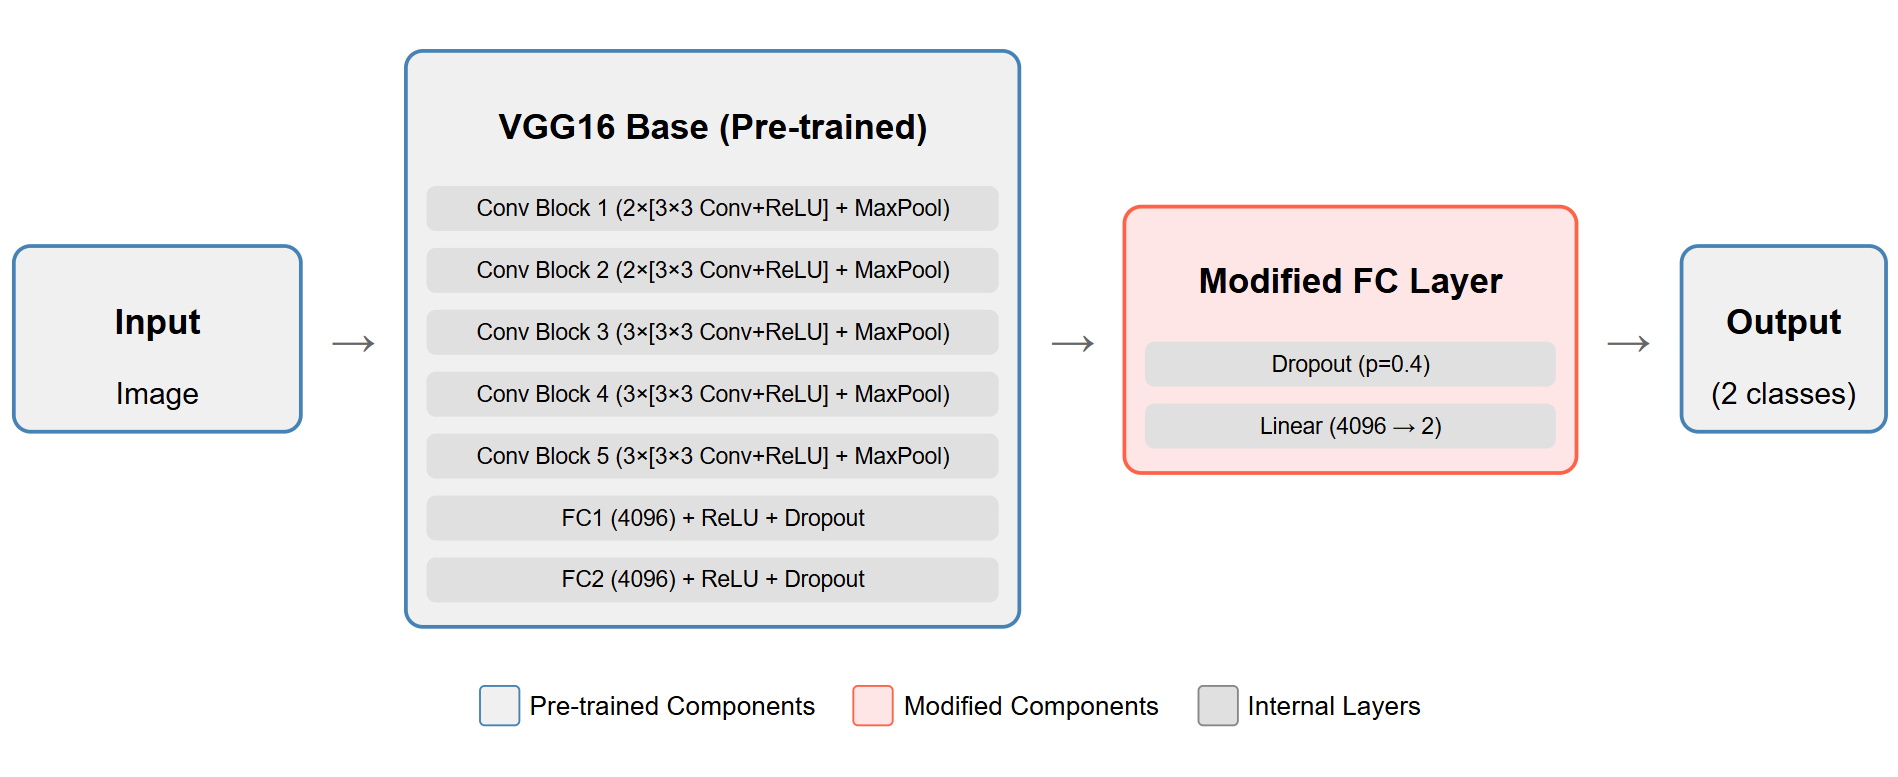
\includegraphics[width=0.8\textwidth]{images/architecture/vgg.png}
    \caption{Architecture of the VGG model}
    \label{fig:vgg_architecture}
\end{figure}


\subsubsection{Theoretical Foundation}

VGG-16, developed by Simonyan and Zisserman (2014) \citep{simonyan2014vgg} at the Visual Geometry Group (VGG) at Oxford, is a 16 layer CNN with 13 convolutional layers followed by 3 fully connected layers known for its deep stack of 3×3 convolutional filters followed by max pooling layers. With approximately 138 million parameters, VGG-16 provides a strong foundation for feature extraction in computer vision tasks although it is computationally exprensive compared to other architectures. Pre-trained on the ImageNet dataset containing over 1.2 million images across 1,000 classes, VGG-16 offers robust initialization weights that facilitate effective knowledge transfer to domain-specific tasks with limited training data.

VGG-16 has demonstrated superior performance in fine-grained classification tasks compared to conventional techniques. Recent studies show that VGG-16 with logistic regression achieved 97.14\% accuracy on specialized datasets like Leaf12, significantly outperforming traditional approaches that combined color channel statistics, texture features, and classic classifiers which only reached 82.38\% accuracy \citep{pearline2019study}. For our specific task of gull species classification, the hierarchical feature representation capabilities of VGG-16 proved particularly effective at capturing the subtle differences in wing patterns and morphological features that distinguish between the target species.

By modifying the final classification layer to match the number of output classes, the VGG16 model can retain its ability to recognize general features and adapt to the unique visual characteristics of different bird species. This approach mirrored in my implementation, aligns with successful methodologies in avian species classification using VGG-16 as demonstrated by Brown et al. (2018), where fine-tuning the architecture by modifying the final classification layer enabled the model to retain general feature recognition capabilities while adapting to species-specific visual characteristics \citep{10533638}.

\subsubsection{Model Adaptation for Fine-Grained Classification}

The VGG architecture followed the common methodology approach mentioned in Section~\ref{sec:common} with a dropout and FC layer  mapping from the original 4096 features to 2 output classes replacing the original 1000-class classifier.

% USEFUL GOOD FOR ALL THE VALUES LIKE OPTIMISER ETC https://ieeexplore.ieee.org/stamp/stamp.jsp?tp=&arnumber=10533638&tag=&tag=1

\subsection{Vision Transformer (ViT) Architecture}

\begin{figure}[H]
    \centering
    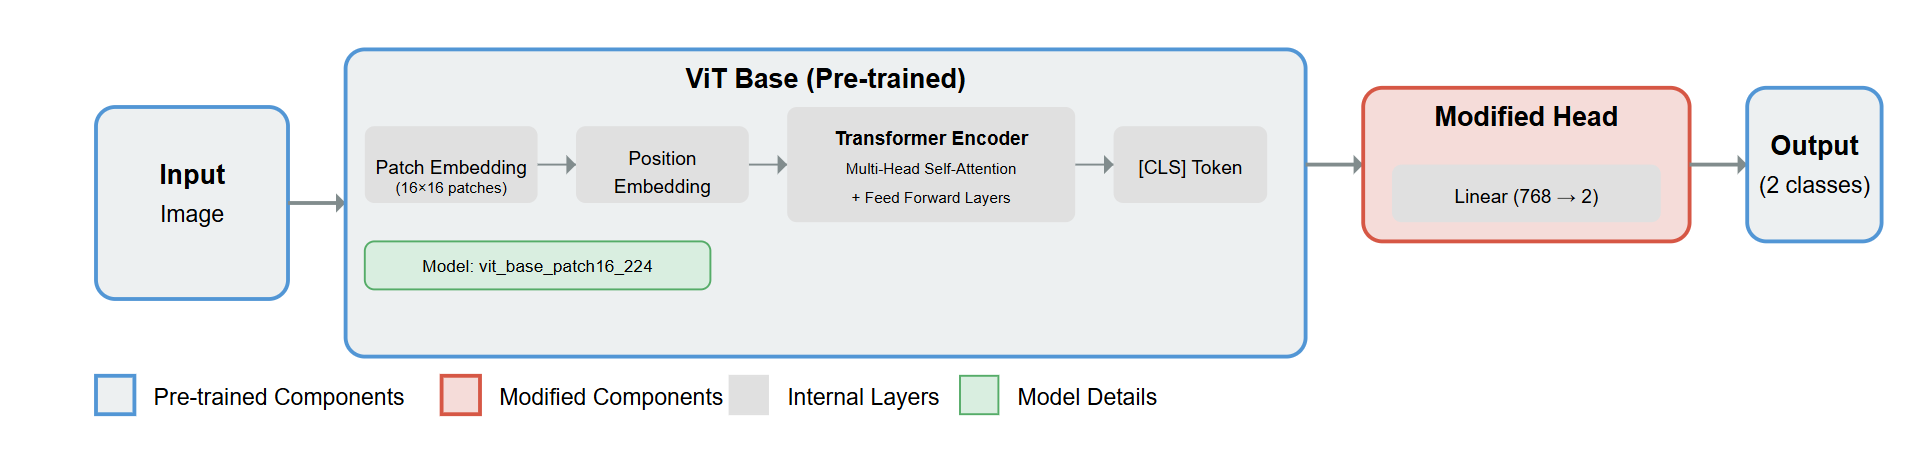
\includegraphics[width=0.8\textwidth]{images/architecture/vit.png}
    \caption{Architecture of the Vision Transformer (ViT) model}
    \label{fig:vit_architecture}
\end{figure}

\subsection{ViT for Fine-Grained Classification}

Vision Transformers (ViT) have emerged as powerful alternatives to convolutional neural networks for visual recognition tasks. First introduced by Dosovitskiy et al. \citep{dosovitskiy2021imageworth16x16words}, ViTs process images as sequences of fixed-size patches, applying transformer-based self-attention mechanisms to model global relationships between image regions. This architecture enables the capture of long-range dependencies within images, making it particularly suitable for fine-grained classification tasks where subtle distinctions between similar classes may depend on relationships between distant image features.

\subsubsection{Vision Transformer Implementation}

For our primary approach, a Vision Transformer was implemented using transfer learning from a pre-trained model with base architecture 'vit\_base\_patch16\_224' pre-trained on ImageNet from the TIMM library \citep{rwightman2021pytorch}. The ViT architecture followed the common methodology approach mentioned in Section~\ref{sec:common}. The model architecture preserves the core self-attention mechanism of ViT while adapting the final classification layer for our specific binary classification task.

\subsubsection{Alternative ViT Implementations}

In addition to our primary implementation, we explored two attention-enhanced architectures for compatibility with Grad-CAM:

\textbf{InterpretableViT}
We developed an InterpretableViT model that incorporates explicit attention mechanisms for improved focus on discriminative features:

\begin{itemize}
    \item Separates the class token from patch tokens
    \item Applies a learned attention layer to generate importance weights for each patch
    \item Combines the class token with attention-weighted patch representations
    \item Employs a multi-layer classifier with dropout regularization
\end{itemize}

By separating the class token from patch tokens and implementing an explicit attention mechanism, the model facilitates more effective application of Grad-CAM, allowing for visualization of discriminative image regions contributing to classification decisions.

% check above referencea and cite as Selvaraju_2019

\paragraph{EnhancedViT}
We also implemented an EnhancedViT that applies attention-based weighting across all tokens:

\begin{itemize}
    \item Processes all tokens (including class token) through an attention mechanism
    \item Generates a single attention-weighted feature representation
    \item Utilizes a specialized classification head with dropout for regularization
\end{itemize}

% https://arxiv.org/pdf/2006.03677 TODO CHECK REF ABOVE

\subsection{Inception v3 Architecture}

\begin{figure}[H]
    \centering
    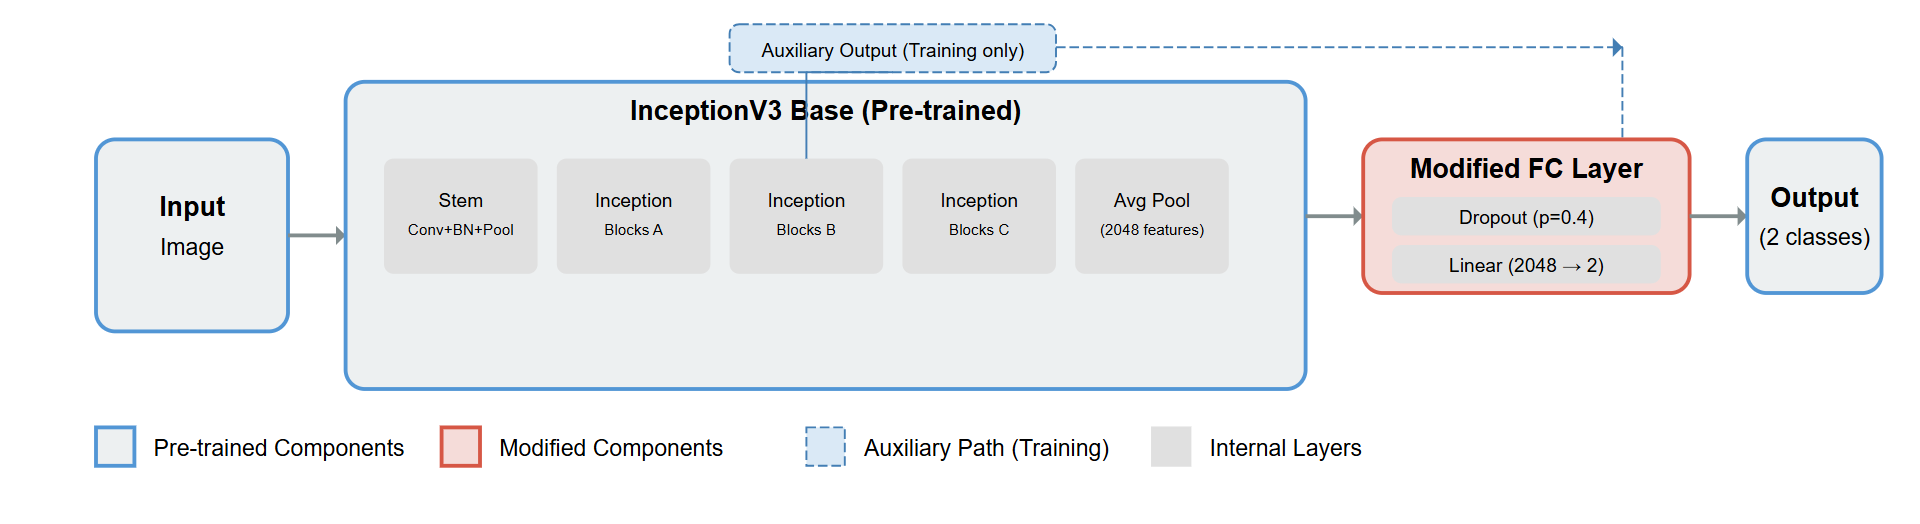
\includegraphics[width=0.8\textwidth]{images/architecture/inception.png}
    \caption{Architecture of the Inception v3 model}
    \label{fig:inception_architecture}
\end{figure}

\subsection*{Theoretical Background}

Inception v3 \citep{szegedy2015rethinkinginceptionarchitecturecomputer} employs a modular design centered around \textit{Inception modules} that process input tensors through multiple parallel convolution pathways with varying receptive fields. This design efficiently captures multi-scale features simultaneously, making it particularly effective for fine-grained classification tasks requiring detection of subtle morphological differences.

The key architectural innovations in Inception v3 that informed our implementation include:
\begin{itemize}
    \item Factorized convolutions that reduce computational complexity while maintaining representational power
    \item Auxiliary classifiers that inject additional gradient signals to mitigate vanishing gradients
    \item Batch normalization for training stability and faster convergence

\end{itemize}

\subsubsection{Model-Specific Implementation Details}

Our implementation adapted the pre-trained Inception v3 model for binary classification with auxiliary outputs. During training, we utilized Inception v3's auxiliary classifier to provide an additional gradient path during backpropagation, which is a distinctive feature of this architecture not found in our other implementations. Mixed precision training with torch.amp.GradScaler() was used to improve computational efficiency without sacrificing accuracy.

\subsection{Residual Network (ResNet-50) Architecture}

\begin{figure}[H]
    \centering
    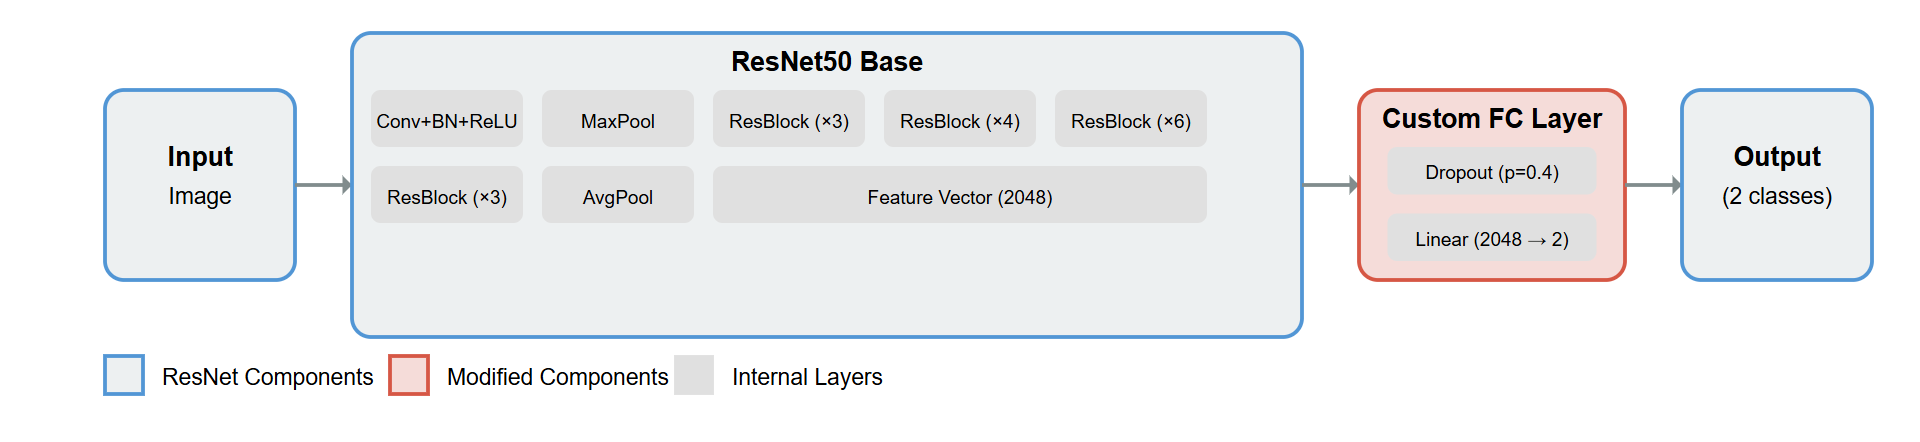
\includegraphics[width=0.8\textwidth]{images/architecture/resnet.png}
    \caption{Architecture of the ResNet-50 model}
    \label{fig:resnet_architecture}
\end{figure}

\subsection*{Theoretical Background}

ResNet-50 \citep{he2016deep} addresses the degradation problem in deep neural networks through the introduction of residual connections (skip connections). These connections enable the network to learn residual mappings rather than direct mappings, allowing for substantially deeper architectures without suffering from vanishing gradients. The residual block can be formulated as:

\begin{equation}
y = \mathcal{F}(x, \{W_i\}) + x
\end{equation}

where $\mathcal{F}$ represents the residual mapping to be learned and $x$ is the identity connection. This formulation makes optimization easier as the network only needs to learn the residual with respect to the identity mapping.

The ResNet architecture followed the common methodology approach mentioned in Section~\ref{sec:common}.

\subsection{Custom CNN with Squeeze-and-Excitation Blocks}

\begin{figure}[H]
    \centering
    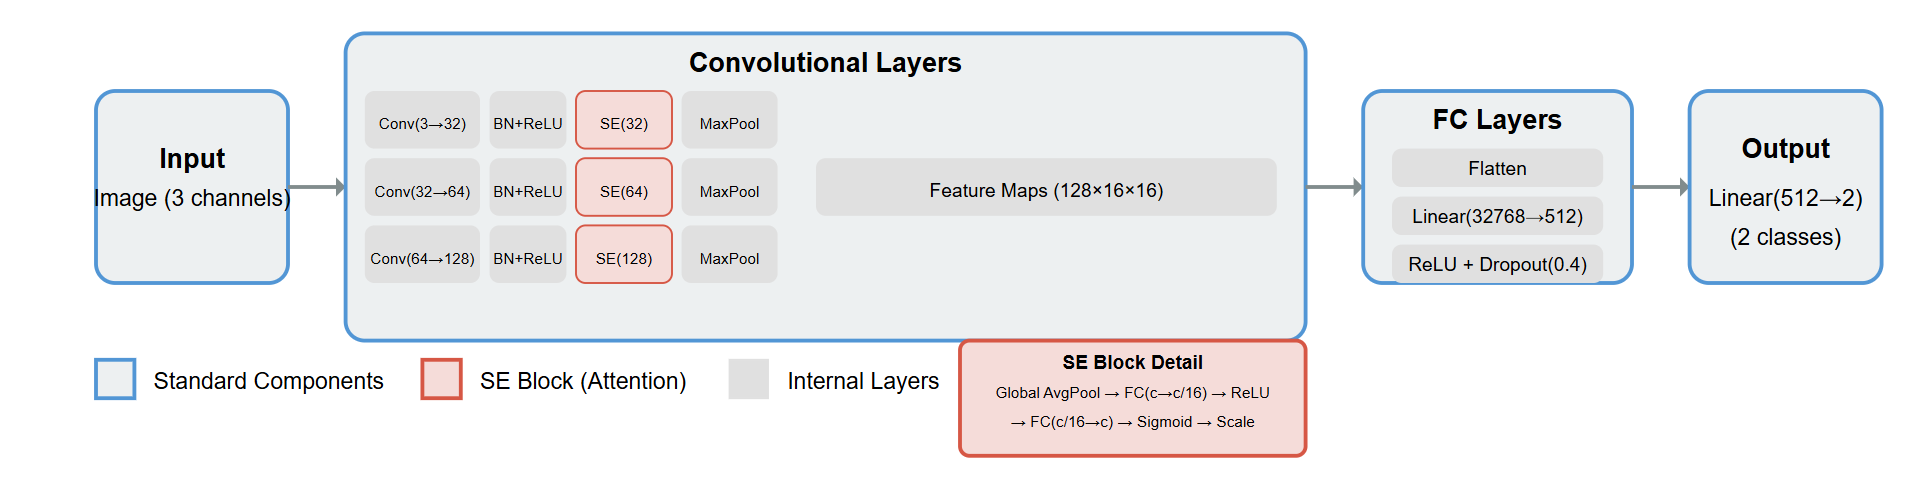
\includegraphics[width=0.8\textwidth]{images/architecture/improvedcnn.png}
    \caption{Architecture of the Custom CNN with Squeeze-and-Excitation Blocks}
    \label{fig:improvedcnn_architecture}
\end{figure}

\subsubsection{Architectural Design}

To address the challenges of limited data and class imbalance in fine-grained classification, we developed a lightweight custom CNN architecture incorporating attention mechanisms. Our approach employs Squeeze-and-Excitation (SE) blocks, which enhance feature representation by modeling channel interdependencies through an attention mechanism. The SE block, as introduced by Hu et al. \citep{Hu_2018_CVPR}, adaptively recalibrates channel-wise feature responses to emphasize informative features while suppressing less useful ones.

The architecture consists of three convolutional blocks, each followed by batch normalization, ReLU activation, and an SE block. The SE block performs two key operations:
\begin{itemize}
    \item \textbf{Squeeze}: Global average pooling across spatial dimensions to generate channel-wise statistics
    \item \textbf{Excitation}: A fully connected layer that produces modulation weights for each channel
\end{itemize}

This channel-wise attention mechanism has been shown to improve model performance with minimal computational overhead \citep{Hu_2018_CVPR}. The SE blocks in our implementation use a reduction ratio of 16, balancing parameter efficiency and representational power.

\subsubsection{Custom CNN-Specific Training Approach}

Unlike the transfer learning approaches used with pre-trained models, our custom CNN was trained from scratch with some specific optimization strategies:

\begin{itemize}
    \item \textbf{Cosine Annealing scheduler}: Our learning rate schedule follows a cosine annealing pattern with a period of 20 epochs, allowing the learning rate to oscillate and potentially escape local minima.
    
% IRRELEVANT (\href{https://arxiv.org/abs/1608.03983}{Loshchilov and Hutter, 2017})
    \item \textbf{Batch normalization:} Used in custom CNN implementations to stabilize learning and improve convergence \citep{ioffe2015batch}.
    
    \item \textbf{Specialized augmentation}: The custom CNN particularly benefited from more aggressive data augmentation strategies to compensate for the lack of pre-trained weights, including stronger rotations and more extensive color jittering than used with the transfer learning models.
\end{itemize}

\section{Model Interpretability Methodologies}

Deep learning models, particularly Convolutional Neural Networks (CNNs) and Vision Transformers (ViTs), are often criticized for their lack of transparency, functioning as "black boxes" wherein the decision-making process remains opaque to human observers. For critical applications like wildlife species classification, understanding how these models arrive at their predictions is essential for establishing trust and validating results. This section outlines the methodologies implemented to visualize and interpret the classification decisions of both the CNN architecture and Vision Transformer (ViT) models used in this study.

\subsection{Gradient-weighted Class Activation Mapping (Grad-CAM)}

Gradient-weighted Class Activation Mapping (Grad-CAM) is a widely adopted visualization technique that produces visual explanations for decisions made by CNN-based models without requiring architectural changes or retraining \citep{Selvaraju_2019}. It generates coarse localization maps highlighting the regions in the input image that significantly influenced the model's prediction for a specific class.

\subsubsection{Theoretical Foundation}

Grad-CAM extends the Class Activation Mapping (CAM) approach \citep{zhou2015learningdeepfeaturesdiscriminative} by utilizing the gradient information flowing into the final convolutional layer of a CNN. Unlike CAM, which requires modifications to the network architecture and retraining, Grad-CAM can be applied to any CNN-based architecture without architectural changes, making it more versatile.

The fundamental principle behind Grad-CAM is that the final convolutional layer in a CNN retains spatial information while encoding high-level semantics. By analyzing how the gradients of a specific class score flow into this layer, Grad-CAM can identify the regions in the input image that are most influential for the prediction.

% \begin{algorithm}
% \caption{Gradient-weighted Class Activation Mapping (Grad-CAM)}
% \begin{algorithmic}[1]
% \Input Input image $I$, CNN model $f$, target class $c$, final convolutional layer feature maps $A^k$
% \Output Heatmap $L_{Grad-CAM}^c$
% \State Perform forward pass on model $f$ with input image $I$ to obtain prediction score $y^c$
% \State Compute gradients of score $y^c$ with respect to feature maps $A^k$: $\frac{\partial y^c}{\partial A^k}$
% \State Apply global average pooling to gradients to obtain importance weights $\alpha_k^c$: 
%        $\alpha_k^c = \frac{1}{Z}\sum_i \sum_j \frac{\partial y^c}{\partial A_{ij}^k}$
% \State Calculate weighted combination of feature maps: 
%        $L_{Grad-CAM}^c = ReLU\left(\sum_k \alpha_k^c A^k\right)$
% \State Normalize $L_{Grad-CAM}^c$ to range [0, 1]
% \State Resize $L_{Grad-CAM}^c$ to input image dimensions
% \Return $L_{Grad-CAM}^c$
% \end{algorithmic}
% \end{algorithm}

The ReLU function is applied to the weighted combination of feature maps to focus only on features that have a positive influence on the class of interest, effectively eliminating features that suppress the class.

\subsubsection{Methodology for CNN models}

In this study, Grad-CAM was implemented for the VGG16 model by targeting the final convolutional layer (features[-1]). The implementation involves several key steps:

\begin{enumerate}
    \item \textbf{Hook Registration}: Forward and backward hooks are registered on the target layer to capture activations during the forward pass and gradients during the backward pass.
    
    \item \textbf{Forward Pass}: The input image is passed through the network to obtain the model's prediction.
    
    \item \textbf{Backpropagation}: The gradient of the score for the target class (either the predicted class or a specified class) with respect to the feature maps of the target layer is computed through backpropagation.
    
    \item \textbf{Global Average Pooling}: These gradients undergo global average pooling to obtain weights indicating the importance of each channel for the target class.
    
    \item \textbf{Weighted Combination}: The weights are applied to the activations of the target layer to create a weighted combination of feature maps.
    
    \item \textbf{ReLU Application}: A ReLU function is applied to the weighted combination to focus only on features that have a positive influence on the class of interest. (NumPy's maximum function is used to retain only positive values.)
    
    \item \textbf{Normalization}: The resulting heatmap is normalized to the range [0, 1] for consistent visualization.
    
    \item \textbf{Visualization}: The heatmap is resized to match the input image dimensions and overlaid on the original image using a colormap (typically 'jet') to highlight regions the model focused on for its prediction.
\end{enumerate}



Similar implementation was implemented for other models: Inceptionv3, ResNet50, and CustomCNN. 

\subsection{Attention Rollout for Vision Transformers}

Vision Transformers process images differently from CNNs, using self-attention mechanisms rather than convolution operations to model relationships between image patches. Therefore, a different approach called Attention Rollout is used to visualize ViT decision-making \citep{abnar2020attention}.

\subsubsection{Theoretical Foundation}

The Attention Rollout method visualizes information flow through the layers of a Transformer model. In Vision Transformers, the input image is divided into fixed-size patches, and each patch is linearly embedded along with position embeddings. A special classification token ([CLS]) is added, and the sequence of embedded patches is processed through multiple layers of self-attention.

Attention Rollout computes a measure of how the [CLS] token attends to each image patch by propagating attention through all layers of the network. This provides insight into which parts of the image the model considers most relevant for classification.

\subsubsection{Methodology for ViT}

The implementation of Attention Rollout for the ViT model follows these steps:

\begin{enumerate}
    \item \textbf{Attention Map Collection}: Forward hooks are registered on each transformer block to collect attention maps during the forward pass of an input image.
    
    \item \textbf{QKV Processing}: For each attention head, the query (Q), key (K), and value (V) matrices are extracted and processed to compute the raw attention weights between different tokens.
    
    \item \textbf{Head Averaging}: Attention weights from all heads in each layer are averaged to get a single attention map per transformer block.
    
    \item \textbf{Attention Rollout Computation}: Starting with an identity matrix, attention maps from each layer are sequentially multiplied to account for how attention propagates through the entire network.
    
    \item \textbf{CLS Token Attention Extraction}: The attention weights from the classification ([CLS]) token to each image patch are extracted, which indicates the importance of each patch for the final classification.
    
    \item \textbf{Reshaping and Visualization}: These weights are reshaped to match the spatial dimensions of the input image (typically 14×14 for ViT-Base with patch size 16) and then upsampled to create a heatmap that can be overlaid on the original image.
\end{enumerate}

While the implementation includes a mechanism for filtering low-attention connections through a discard ratio parameter, this feature was not utilized in the final analysis (set to 0.0), focusing instead on the complete attention distribution across all patches.

\subsection{Grad-CAM for Vision Transformers}

In addition to Attention Rollout, this study also implements Grad-CAM for Vision Transformers to provide a more direct comparison with the CNN-based visualizations. Two variants of Grad-CAM for ViT were implemented: Enhanced ViT and Interpretable ViT, each with specific architectural modifications to facilitate interpretation.

\subsection{Enhanced ViT Implementation}

The Enhanced ViT approach modifies the standard ViT architecture to facilitate Grad-CAM visualization:

\begin{itemize}
\item \textbf{Model Architecture:} The Enhanced ViT model utilizes the base ViT by replacing the original classification head with an identity layer, preserving the full token representation from the transformer blocks.

\item \textbf{Attention Mechanism:} An attention layer computes scalar importance scores for all tokens (including both [CLS] and patch tokens), which are then normalized through a softmax operation to produce attention weights.

\item \textbf{Feature Integration:} These attention weights are applied to the token features through a weighted sum operation, creating a single feature vector that represents the entire image with emphasis on the most important regions.

\item \textbf{Gradient Recording:} The model registers hooks to capture token features during the forward pass and their gradients during backpropagation, essential for the Grad-CAM calculation.

\item \textbf{Grad-CAM Computation:} For visualization, the class token is excluded, and only patch tokens (corresponding to image regions) are considered. The tokens and gradients are reshaped from the sequence format back to a 2D spatial grid to recover the image structure.

\item \textbf{Activation Map Generation:} Following standard Grad-CAM procedure, channel-wise weights are computed from gradients and applied to token features to create the final activation map highlighting discriminative regions.
\end{itemize}

\subsection{Interpretable ViT with Feature Concatenation}

The Interpretable ViT variant employs a feature concatenation approach that enhances interpretability:

\begin{itemize}
\item \textbf{Feature Extraction:} The implementation first extracts features from the base ViT model, producing a sequence of token embeddings.

\item \textbf{Token Separation:} After feature extraction, the [CLS] token and patch tokens are explicitly separated for differential processing:
\begin{align}
\text{cls\_token} &= \text{tokens}[:, 0, :] \\
\text{patch\_tokens} &= \text{tokens}[:, 1:, :]
\end{align}

\item \textbf{Attention Weighting:} An attention layer computes importance weights specifically for the patch tokens, determining each patch's contribution to the final representation:
\begin{align}
\text{attn\_scores} &= \text{attention\_layer}(\text{patch\_tokens}) \\
\text{attn\_weights} &= \text{softmax}(\text{attn\_scores}, \text{dim}=1)
\end{align}

\item \textbf{Weighted Representation:} The patch tokens are combined using these attention weights to form a single weighted feature vector:
\begin{align}
\text{weighted\_patch} = \sum_{i} \text{attn\_weights}_i \cdot \text{patch\_tokens}_i
\end{align}

\item \textbf{Feature Concatenation:} The [CLS] token (providing global context) and the weighted patch features (providing localized information) are concatenated to form a comprehensive representation:
\begin{align}
\text{combined} = [\text{cls\_token}; \text{weighted\_patch}]
\end{align}

\item \textbf{Classifier Architecture:} To accommodate this concatenated representation, the classifier's first layer accepts double the embedding dimension as input:
\begin{align}
\text{classifier} = \text{LayerNorm}(\text{embed\_dim} \times 2) \rightarrow \text{Dropout} \rightarrow \text{Linear} \rightarrow \ldots
\end{align}

\item \textbf{Grad-CAM Visualization:} During Grad-CAM computation, gradients flow back through this architecture, capturing how both global context and local features influence the classification decision.
\end{itemize}

Both approaches enable visualization of the ViT's decision-making process using gradient information, but with different mechanisms for integrating token features and attention weights. The Enhanced ViT applies attention across all tokens before classification, while the Interpretable ViT explicitly separates and recombines different types of features to provide a more structured view of the classification process.

By implementing these complementary interpretability techniques, this research provides insights into how different neural network architectures—traditional CNNs and modern Transformers—approach the same classification task and what are the distinguishing features between the two classes. The visualizations reveal different feature priorities and decision strategies that each architecture employs, contributing to a deeper understanding of model behavior.


% \begin{itemize}
%     \item \textbf{Confidence Calculation}: Computing the softmax probability for the predicted class to indicate the model's confidence.
    
%     \item \textbf{Misclassification Analysis}: For incorrectly classified images, both the original image and Grad-CAM visualization are saved with annotations indicating the true and predicted classes.
    
%     \item \textbf{Three-Panel Visualization}: Creating a standardized visualization with the original image, the Grad-CAM heatmap, and the overlay for easy comparison.
% \end{itemize}



% \subsection{Implementation Details}

% The interpretability frameworks were implemented with the following technical considerations:

% \subsubsection{Grad-CAM for VGG16}
% \begin{itemize}
%     \item \textbf{Target Layer}: The last convolutional layer of VGG16 (features[-1])
%     \item \textbf{Gradient Calculation}: Using PyTorch's autograd functionality for backpropagation
%     \item \textbf{Output Format}: Three-panel visualization with original image, Grad-CAM heatmap, and overlay
%     \item \textbf{Confidence Annotation}: Each visualization includes the model's confidence percentage
%     \item \textbf{Organization}: Images organized by class and correctness of prediction
% \end{itemize}

% \subsubsection{Attention Rollout for ViT}
% \begin{itemize}
%     \item \textbf{Model Type}: Vision Transformer Base model with 16×16 patch size
%     \item \textbf{Attention Collection}: Forward hooks on all self-attention blocks
%     \item \textbf{QKV Extraction}: Capturing query, key, and value matrices for attention computation
%     \item \textbf{Discard Ratio}: Configurable threshold (set to 0.0) to filter out low-attention areas
%     \item \textbf{Rollout Computation}: Sequential multiplication of attention maps across layers
% \end{itemize}

% \subsubsection{Grad-CAM for ViT}
% \begin{itemize}
%     \item \textbf{Model Architecture}: Custom InterpretableViT with token feature extraction
%     \item \textbf{Gradient Hooks}: Custom hooks to capture token features and their gradients
%     \item \textbf{Attention Layer}: Additional attention mechanism to weight patch tokens
%     \item \textbf{Feature Combination}: Concatenation of class token and weighted patch features
%     \item \textbf{Visualization}: Consistent with the VGG16 Grad-CAM approach for comparison
% \end{itemize}

% \appendix
% \section{Additional Interpretability Techniques}
% \label{appendix:add_interpret}

% In addition to the Grad-CAM method discussed in the main sections of this report, several other interpretability techniques were explored during this research. While not featured prominently in the main analysis, these methods offer complementary perspectives on model decision-making.

% \subsection{DeepLIFT}

% DeepLIFT (Deep Learning Important FeaTures) was implemented using the Captum library for the VGG16 and ViT models. This technique compares activations against a reference baseline (typically zeros) to determine feature importance:

% \begin{itemize}
%     \item A zero baseline tensor is created as a reference point
%     \item Attribution scores are calculated comparing actual activations to this baseline
%     \item Channel-wise attributions are aggregated and normalized for visualization
%     \item Color maps are applied to create interpretable heatmaps
% \end{itemize}

% While DeepLIFT provides more theoretically grounded attributions than simple gradient methods, it was not extended to all models due to it not being used as frequently by others as other techniques such as grad cam/
% \subsection{Saliency Maps}

% Basic saliency maps were implemented for both VGG16 and Vision Transformer models:

% \begin{itemize}
%     \item Input tensors are configured to track gradients
%     \item Forward and backward passes compute gradients from prediction to input
%     \item Absolute values of gradients reveal input sensitivity
%     \item Channel-wise maximum operations create single-channel visualizations
% \end{itemize}


% % This paper examines saliency methods, which are explanation techniques designed to highlight relevant features in inputs (particularly images) that influence a machine learning model's predictions. The authors propose a methodology to evaluate whether these explanation methods are actually providing meaningful insights about the model and data. Their key findings include:

% % Many popular saliency methods fail basic "sanity checks" - they produce explanations that are independent of model parameters and training data.
% % The authors propose two randomization tests to evaluate explanation methods:

% % Model parameter randomization test: Compares explanations from a trained model vs. a randomly initialized model
% % Data randomization test: Compares explanations from a model trained on proper data vs. one trained on randomly permuted labels


% % Several widely used methods (Guided BackProp and Guided GradCAM) fail these tests, meaning they can't provide insights about the model or data relationships.
% % Some methods (standard Gradients and GradCAM) pass the tests, suggesting they are more reliable.
% % The authors demonstrate that some saliency methods produce outputs visually similar to simple edge detectors, which require neither training data nor model knowledge.

% % The paper warns that visual assessment alone can be misleading when evaluating explanation methods. Methods that fail their proposed tests are inadequate for tasks like finding data outliers, explaining model relationships, or debugging models. The authors support their findings with theoretical analysis of linear models and simple convolutional neural networks.
% \subsection{Integrated Gradients for Vision Transformers}

% For the Vision Transformer model specifically, Integrated Gradients was implemented using Captum:

% \begin{itemize}
%     \item Path integrals are approximated between baseline and input images
%     \item 50 interpolation steps were used for the approximation
%     \item Attributions are processed to align with spatial image dimensions
%     \item Results are normalized for consistent visualization
% \end{itemize}

% While theoretically sound, Integrated Gradients requires significantly more computation time than Grad-CAM. Additionally, the literature review indicated that Grad-CAM adaptations for Vision Transformers often provide more intuitive visualizations for classification tasks \cite{chefer2021transformer}.

% \subsection{Guided Backpropagation for Vision Transformers}

% Guided Backpropagation was adapted specifically for Vision Transformers:

% \begin{itemize}
%     \item Modified gradient flow during backpropagation highlights positive influences
%     \item Implementation uses Captum's GuidedBackprop with model-specific wrappers
%     \item Results are post-processed to create single-channel visualizations
% \end{itemize}

% This method produces visually cleaner results than standard saliency maps but lacks the localization capabilities of Grad-CAM. Additionally, research has shown that guided backpropagation may highlight input patterns rather than decision-relevant features \cite{nie2018theoretical}.

% \subsection{Conclusion on Additional Methods}

% These additional interpretability techniques were implemented primarily for exploration and comparison. Grad-CAM was selected as the primary visualization method for the main analysis due to its:

% \begin{itemize}
%     \item Widespread adoption in the literature
%     \item Consistent performance across model architectures
%     \item Ability to produce class-discriminative visualizations
%     \item Better localization of discriminative regions
%     \item Lower computational requirements
%     \item Stronger theoretical foundation compared to simple gradient methods
% \end{itemize}

% The implementation details and experimental results for these additional techniques are preserved here to document the comprehensive approach taken toward model interpretability in this research.

% Though straightforward to implement, saliency maps,  guided backpropagation were not highlighted in the main analysis as they can be noisy and lack the class-discriminative properties of Grad-CAM. Additionally, as noted by \cite{Adebayo2018}, simple gradient methods sometimes fail sanity checks that Grad-CAM passes.

% 3. Of the methods tested, Gradients and GradCAM pass the sanity checks, while Guided BackProp and
% Guided GradCAM are invariant to higher layer parameters; hence, fail.
% 4. Consequently, our findings imply that the saliency methods that fail our proposed tests are incapable
% of supporting tasks that require explanations that are faithful to the model or the data generating
% process.  \href{https://arxiv.org/pdf/1810.03292}{(Guided and saliency not good)}

% TODO
% \appendix
\section{Additional Interpretability Techniques}
\label{appendix:add_interpret}

In addition to the Grad-CAM and attention rollout methods discussed in the main sections of this report, several other interpretability techniques were explored during this research.

\subsection{DeepLIFT}

DeepLIFT (Deep Learning Important FeaTures) \Citep{shrikumar2017learning} was implemented using the Captum library for the VGG16 and ViT models. This technique compares activations against a reference baseline (typically zeros) to determine feature importance:

\begin{itemize}
\item A zero baseline tensor is created as a reference point
\item Attribution scores are calculated comparing actual activations to this baseline
\item Channel-wise attributions are aggregated and normalized for visualization
\end{itemize}

While DeepLIFT provides theoretically grounded attributions, it was not adopted for the main analysis due to its limited adoption in the literature compared to prevalent techniques like Grad-CAM.

\subsection{Saliency Maps}

\begin{itemize}
\item Gradients of predictions with respect to input pixels are computed
\item Absolute values of gradients are visualized as sensitivity maps
\end{itemize}

\subsection{Integrated Gradients for Vision Transformers}

Integrated Gradients was implemented for ViT using 50 interpolation steps:

\begin{itemize}
    \item Path integrals are approximated between baseline and input images
    \item 50 interpolation steps were used for the approximation
    \item Attributions are processed to align with spatial image dimensions
    \item Results are normalized for consistent visualization
\end{itemize}

\subsection{Guided Backpropagation for ViT}

\begin{itemize}
    \item Modified gradient flow during backpropagation highlights positive influences
    \item Implementation uses Captum's GuidedBackprop with model-specific wrappers
    \item Results are post-processed to create single-channel visualizations
\end{itemize}


\subsection{Justification for Grad-CAM}

Grad-CAM was chosen as the primary interpretability method for this study due to its unique advantages over the alternatives:

\begin{itemize}
\item \textbf{Theoretical Robustness}: Grad-CAM passes sanity checks (e.g., parameter randomization tests) that methods like Guided Backpropagation, saliency maps and Guided Grad-CAM fail \citep{Adebayo2018}. Findings of \citep{Adebayo2018} implied that the saliency methods that failed their proposed tests were incapable of supporting tasks that require explanations that are faithful to the model or the data generating process.
\item \textbf{Class-Discriminative}: Grad-CAM highlights regions relevant to specific predicted classes \citep{Selvaraju_2019}.
\item \textbf{Architecture Flexibility}: Works consistently across CNNs (e.g., VGG16, ResNet) and adapted Vision Transformers.
\item \textbf{Computational Efficiency}: Requires only a single backward pass per class, unlike path-based methods (e.g., Integrated Gradients).
\item \textbf{Empirical Validation}: Grad-CAM is supported by extensive literature \citep{Selvaraju_2019, chefer2021generic} demonstrating its effectiveness for classification tasks.
\end{itemize}
% Add these to your bibliography
% \bibitem{adebayo2018sanity} Adebayo, J., Gilmer, J., Muelly, M., Goodfellow, I., Hardt, M., \& Kim, B. (2018). Sanity checks for saliency maps. In Advances in Neural Information Processing Systems.
% \bibitem{chefer2021transformer} Chefer, H., Gur, S., \& Wolf, L. (2021). Transformer interpretability beyond attention visualization. In Proceedings of the IEEE/CVF Conference on Computer Vision and Pattern Recognition.
% \bibitem{nie2018theoretical} Nie, W., Zhang, Y., \& Patel, A. (2018). A theoretical explanation for perplexing behaviors of backpropagation-based visualizations. In International Conference on Machine Learning.

\section{Feature Analysis for Fine-Grained Gull Classification}

\subsection{Image Preprocessing and Region-Based Segmentation}
A multi-stage approach was employed to extract and analyze region-specific features.

\subsubsection{Image Selection}
From the Stage 3 dataset, 200 high-resolution images (100 per species) were selected based on the following criteria:
\begin{itemize}
\item Correct classification by the best-performing VGG-16 model
\item Prominent Grad-CAM activations in wing or wingtip regions
\item Clear visibility of upperwing or wingtip in the image
\item High resolution image
\end{itemize}

\subsubsection{Manual Segmentation}
Using Adobe Photoshop, segmentation masks with color-coded regions were created with a specific color for each type of region: wing, wingtip, and head.

\subsubsection{Normalization}
Min-max normalization\citep{monzon_image_normalization} (0-255) was applied to grayscale conversions using OpenCV's \texttt{NORM\_MINMAX}.
This helped standardize intensity values and mitigate the effects of differing lighting conditions ensuring that pixel intensity values were scaled consistently across the dataset, providing a reliable foundation for subsequent region-based analysis.

\subsubsection{Region Extraction}

Using OpenCV's \texttt{inRange} for color-based thresholding, pixels that match each target colour were identified to create binary masks where the region of interest is set to 255 (white) and the rest to 0 (black). These binary masks were then applied to the original images using bitwise operations to extract the actual pixel values of the bird's regions—such as the wing, wingtip, head, and body—for subsequent analysis.

% \section{Local Binary Pattern Gemini}

% \section{Methodology}

% \subsection{Local Binary Pattern Analysis}

% The texture analysis methodology employs Local Binary Patterns (LBP) to quantify the textural characteristics of gull feather regions. LBP is a powerful texture descriptor that captures local spatial structure by comparing each pixel with its neighboring pixels.



% We implemented uniform LBP patterns, which account for transitions between 0s and 1s in the binary representation, thereby capturing fundamental texture elements like edges and corners while reducing dimensionality.

% \subsubsection{Feature Extraction}

% From the LBP computation, three primary feature histograms were extracted:

% \begin{enumerate}
%     \item \textbf{LBP Histogram}: Distribution of LBP codes across the region of interest
    
%     \item \textbf{Ones Histogram}: Distribution of the number of 1s in each LBP code, calculated as:
%     \begin{equation}
%     H_{\text{ones}}(i) = \sum_{j=0}^{N-1} [b(j) = i]
%     \end{equation}
%     where $b(j)$ represents the number of 1s in pattern $j$, and $[\cdot]$ is the Iverson bracket
    
%     \item \textbf{Transitions Histogram}: Distribution of 0-to-1 or 1-to-0 transitions in each LBP code:
%     \begin{equation}
%     H_{\text{trans}}(i) = \sum_{j=0}^{N-1} [t(j) = i]
%     \end{equation}
%     where $t(j)$ counts the transitions in pattern $j$
% \end{enumerate}

% \subsection{Texture Feature Quantification}

% From these histograms, several texture properties were calculated to characterize the regions:

% \begin{enumerate}
%     \item \textbf{Entropy}: Measures randomness in texture patterns
%     \begin{equation}
%     E = -\sum_{i} h(i) \log_2 h(i)
%     \end{equation}
%     where $h(i)$ is the normalized histogram value at bin $i$
    
%     \item \textbf{Energy}: Measures uniformity of texture
%     \begin{equation}
%     U = \sum_{i} h(i)^2
%     \end{equation}
    
%     \item \textbf{Contrast}: Measures intensity variations
%     \begin{equation}
%     C = \sum_{i} (i - \mu)^2 h(i)
%     \end{equation}
%     where $\mu$ is the mean value of the histogram
    
%     \item \textbf{Homogeneity}: Measures closeness of distribution
%     \begin{equation}
%     H = \sum_{i} \frac{h(i)}{1 + |i - \mu|}
%     \end{equation}
% \end{enumerate}

\subsection{Local Binary Pattern Analysis}

Local Binary Patterns (LBP) constitute a robust and computationally efficient texture analysis technique, originally proposed by Ojala et al. \Citep{1017623}. LBP characterizes local image texture by comparing each pixel's intensity with its surrounding neighbors, generating a binary code that summarizes the local structure. This descriptor is particularly advantageous for biological image analysis due to several key properties:

\begin{itemize}
    \item Robustness to monotonic grayscale variations, enhancing resilience to changing illumination conditions.
    \item Rotation invariance when using specific LBP variants or derived features (1s and transition histograms)
    \item Ability to capture fine-scale micro-patterns potentially imperceptible to human vision.
\end{itemize}

To investigate subtle textural differences between Slaty-backed Gulls and Glaucous-winged Gulls, Local Binary Pattern (LBP) analysis was conducted on three anatomical regions: wing, wingtip, and head.

\subsubsection{LBP Computation}

% For a given pixel at position $(x_c, y_c)$ with intensity $g_c$, the LBP value is computed by comparing it with $P$ neighbors at radius $R$ using the following equation:

% \begin{minipage}{0.48\textwidth}
% \begin{equation}
% \text{LBP}_{P,R}(x_c, y_c) = \sum_{p=0}^{P-1} s(g_p - g_c) \cdot 2^p
% \end{equation}
% where:
% \begin{itemize}
%     \item $g_p$ is the intensity of the neighbor pixel $p$
%     \item $s(x)$ is the step function defined as:
% \end{itemize}
% \end{minipage}
% \hfill
% \vrule
% \hfill
% \begin{minipage}{0.48\textwidth}
% \begin{equation}
% s(x) = 
% \begin{cases} 
% 1, & \text{if } x \geq 0 \\ 
% 0, & \text{if } x < 0 
% \end{cases}
% \end{equation}
% \end{minipage}

% \vspace{1.5em}

% Two variants were implemented:
% \begin{itemize}
%     \item \textbf{Default LBP}: Standard implementation without uniformity constraints
%     \item \textbf{Uniform LBP}: Considers patterns with $\leq 2$ bitwise transitions
% \end{itemize}

% For the final results, the default LBP variant was selected since default histogram retains all possible LBP codes, providing a comprehensive representation of local texture patterns. Consequently, it facilitates the direct calculation of derived features such as the number of ones and the number of transitions per pattern, as these statistics can be computed from the complete set of binary codes present in the default histogram. This approach ensures that no potentially discriminative texture information is excluded, thereby supporting a more detailed and flexible analysis of texture complexity and structure across the studied regions.

For a given pixel at position $(x_c, y_c)$ with intensity $g_c$, the LBP value is computed by comparing it with $P$ neighbors at radius $R$ using the following equation:

\begin{equation}
\text{LBP}_{P,R}(x_c, y_c) = \sum_{p=0}^{P-1} s(g_p - g_c) \cdot 2^p
\end{equation}

where:
\begin{itemize}
    \item $g_p$ is the intensity of the neighbor pixel $p$
    \item $s(x)$ is the step function defined as:
\end{itemize}

\begin{equation}
s(x) = 
\begin{cases}
1, & \text{if } x \geq 0 \\
0, & \text{if } x < 0
\end{cases}
\end{equation}

\begin{equation}
\text{LBP}_{P,R} = \sum_{p=0}^{P-1} s(g_p - g_c) \cdot 2^p,\quad s(x) = 
\begin{cases}
1, & x \geq 0 \\
0, & x < 0
\end{cases}
\end{equation}

Two variants were implemented:
\begin{itemize}
    \item \textbf{Default LBP}: Standard implementation without uniformity constraints
    \item \textbf{Uniform LBP}: Considers patterns with $\leq 2$ bitwise transitions
\end{itemize}

\subsubsection{Feature Extraction}
\label{subsec:feature_extraction}

Three feature histograms were derived from LBP codes:

\begin{enumerate}
    \item \textbf{LBP Histogram}: Raw distribution of LBP codes
    
    \item \textbf{Ones Histogram}: Frequency of patterns with $n$ ones:
    \begin{equation}
    H_{\text{ones}}(i) = \sum_{j=0}^{N-1} [b(j) = i]
    \end{equation}
    
    \item \textbf{Transitions Histogram}: Frequency of patterns with $m$ transitions:
    \begin{equation}
    H_{\text{trans}}(i) = \sum_{j=0}^{N-1} [t(j) = i]
    \end{equation}
\end{enumerate}

Texture properties were calculated from these histograms:

\begin{enumerate}
    \item \textbf{Entropy}: Measures randomness in texture patterns
    \begin{equation}
    E = -\sum_{i} h(i) \log_2 h(i)
    \end{equation}
    where $h(i)$ is the normalized histogram value at bin $i$
    
    \item \textbf{Energy}: Measures uniformity of texture
    \begin{equation}
    U = \sum_{i} h(i)^2
    \end{equation}
    
    \item \textbf{Contrast}: Measures intensity variations
    \begin{equation}
    C = \sum_{i} (i - \mu)^2 h(i)
    \end{equation}
    where $\mu$ is the mean value of the histogram
    
    \item \textbf{Homogeneity}: Measures closeness of distribution
    \begin{equation}
    H = \sum_{i} \frac{h(i)}{1 + |i - \mu|}
    \end{equation}
\end{enumerate}


\subsubsection{Comparative Analysis Implementation}

To quantify the differences between species, the implementation calculates several distribution similarity metrics:

\begin{enumerate}
    \item \textbf{KL Divergence}: A symmetric version of the Kullback-Leibler divergence that measures how one probability distribution diverges from another

    \item \textbf{Earth Mover's Distance}: Measures the minimum ``work'' required to transform one histogram into another, considering the distance between bins

    \item \textbf{Chi-Square Distance}: A statistical test that measures the difference between observed and expected frequency distributions

    \item \textbf{Jensen-Shannon Distance}: A symmetric and smoothed version of the KL divergence with better numerical properties
\end{enumerate}

Each metric captures different aspects of distribution similarity, providing a robust framework for comparing texture patterns between species.

% \subsubsection{Discriminative Power Analysis}

% A systematic assessment of discriminative power for different texture features and regions is performed by calculating percentage differences between species for each texture property and region. This analysis identifies which features and regions exhibit the most significant differences between species.

% For each region and property combination, the implementation:
% \begin{enumerate}
%     \item Extracts the property value for each species
%     \item Calculates the percentage difference
%     \item Ranks the region-property pairs by their discriminative power
% \end{enumerate}

% This approach enables the identification of the most promising texture characteristics for species differentiation.

% \subsubsection{Dimensionality Reduction and Visualization}

% The implementation uses Principal Component Analysis (PCA) to visualize the high-dimensional LBP feature space in two dimensions:

% \begin{enumerate}
%     \item Standardize the feature data
%     \item Apply PCA with 2 components
%     \item Create scatter plots colored by species
%     \item Calculate and display variance explained
% \end{enumerate}

% This dimensionality reduction approach provides intuitive visualization of class separability and validates the discriminative power of the extracted features.

% \subsubsection{Implementation Workflow}

% The complete analysis pipeline consists of two main modules:

% \begin{enumerate}
%     \item \textbf{Feature Extraction Module}:
%     \begin{itemize}
%         \item Loads original and segmentation images
%         \item Extracts and processes each anatomical region
%         \item Computes LBP features and abstract pattern features
%         \item Saves features to CSV files for further analysis
%     \end{itemize}

%     \item \textbf{Analysis Modules}:
%     \begin{itemize}
%         \item Loads extracted features
%         \item Calculates advanced texture statistics
%         \item Performs comparative analysis between species
%         \item Generates visualizations and statistical reports
%         \item Identifies the most discriminative features
%     \end{itemize}
% \end{enumerate}

This modular approach facilitates efficient processing of large image datasets and enables iterative refinement of the analysis parameters.

\subsubsection{Discriminative Power Analysis}
A systematic assessment of discriminative power for different texture features and regions is performed by calculating percentage differences between species for each texture property and region. This analysis identifies which features and regions exhibit the most significant differences between species. For each region and property combination, the implementation extracts the property value for each species, calculates the percentage difference, and ranks the region-property pairs by their discriminative power. This approach enables the identification of the most promising texture characteristics for species differentiation.

\subsubsection{Dimensionality Reduction and Visualization}
The implementation uses Principal Component Analysis (PCA) to visualize the high-dimensional LBP feature space in two dimensions. The process involves standardizing the feature data, applying PCA with 2 components, creating scatter plots colored by species, and calculating and displaying variance explained. This dimensionality reduction approach provides intuitive visualization of class separability and validates the discriminative power of the extracted features.

\subsubsection{Implementation Workflow}
The complete analysis pipeline consists of two main modules. The Feature Extraction Module loads original and segmentation images, extracts and processes each anatomical region, computes LBP features and abstract pattern features, and saves features to CSV files for further analysis. The Analysis Modules load extracted features, calculate advanced texture statistics, perform comparative analysis between species, generate visualizations and statistical reports, and identify the most discriminative features. This modular approach facilitates efficient processing of large image datasets and enables iterative refinement of the analysis parameters.

\subsubsection{Validation Approach}
The implementation includes a few validation mechanisms: normalized histograms to account for varying region sizes, multiple comparison metrics to ensure robust similarity assessment, and quantitative comparison metrics (KL divergence, percentage differences) to assess feature differences.

\section{Wing and Wingtip Intensity Analysis}
% \href{https://doi.org/10.1111/j.1474-919X.2007.00703.x}{(Olsen and Larsson, 2007)}
The interpretability analysis of our VGG model indicated a strong focus on wing and wingtip regions when differentiating between Slaty-backed Gulls and Glaucous-winged Gulls. This aligns with ornithological knowledge, as these species exhibit distinct differences in wing coloration patterns, particularly in the wing and wingtip regions. To quantitatively validate these differences and check whether the differences are significant, an in-depth image analysis was conducted focusing on these critical regions.

% This aligns with known plumage differences documented in ornithological studies \cite{olsen2007gulls}.

% TODO
We employed a multi-stage approach to extract and analyze region-specific features:

\subsection{Feature Extraction Pipeline}
The Python pipeline executed these steps for each image:
\begin{enumerate}
    \item \textbf{Region-Specific Analysis}: Calculated intensity statistics (mean, median, std, skewness, kurtosis, minimum and maximum values) per region
 
    \item \textbf{Wingtip Characterization}:
    \begin{itemize}
        \item Analyzed intensity distribution across 25 bins (10-unit intervals):
        \begin{verbatim}
        intensity_ranges = [
            (0,10), (10,20), ..., (240,255)  # 25 total bins
        ]
        \end{verbatim}
        \item Quantified dark pixels using thresholds: $<30$, $<40$, $<50$, $<60$ intensity
    \end{itemize}
    \item \textbf{Wing-Wingtip Difference}
    \begin{itemize}
        \item Computed percentage of wingtip pixels darker than mean wing intensity of the bird.
        \item \textbf{Thresholds}: Calculated the proportion of wingtip pixels exceeding specific difference thresholds (10, 20, ..., 100) compared to the mean wing intensity, quantifying the contrast between regions.
    \end{itemize}
\end{enumerate}

\subsection{Statistical Testing Methodology}
For quantitative comparison between the two gull species, we employed Welch's t-test (unequal variances t-test) to analyze the differences in wing and wingtip intensity values. This test was selected as it does not assume equal variances between groups, making it more robust for our dataset.

The test statistic was calculated as:  
\begin{equation}  
t = \frac{\bar{X}_1 - \bar{X}_2}{\sqrt{\frac{s_1^2}{n_1} + \frac{s_2^2}{n_2}}}  
\end{equation}  
where $\bar{X}_i$, $s_i^2$, and $n_i$ are the means, sample variances, and sizes for Slaty-backed and Glaucous-winged Gulls, respectively. Degrees of freedom ($\nu$) were approximated using the Welch–Satterthwaite equation.  

% The test statistic was calculated as:
% \begin{equation}
% t = \frac{\bar{X}_1 - \bar{X}_2}{\sqrt{\frac{s_1^2}{n_1} + \frac{s_2^2}{n_2}}}
% \end{equation}

% Where:
% \begin{itemize}
%     \item $\bar{X}_1$ = Mean intensity for Slaty-backed Gulls
%     \item $\bar{X}_2$ = Mean intensity for Glaucous-winged Gulls
%     \item $s_1^2$ = Sample variance for Slaty-backed Gulls
%     \item $s_2^2$ = Sample variance for Glaucous-winged Gulls
%     \item $n_1$ = Sample size for Slaty-backed Gulls
%     \item $n_2$ = Sample size for Glaucous-winged Gulls
% \end{itemize}

The degrees of freedom were approximated using the Welch--Satterthwaite equation:
\begin{equation}
\nu \approx \frac{\left(\frac{s_1^2}{n_1} + \frac{s_2^2}{n_2}\right)^2}{\frac{(s_1^2/n_1)^2}{n_1-1} + \frac{(s_2^2/n_2)^2}{n_2-1}}
\end{equation}

Where $\nu$ represents the degrees of freedom used to determine the critical values for the t-distribution.

All statistical tests were implemented using SciPy's \texttt{stats.ttest\_ind()} function with \texttt{equal\_var=False} parameter to specify Welch's t-test. These statistical analyses allowed us to find and objectively validate whether the differences found through the analysis in areas highlighted by Grad-CAM (wing and wingtip) between species are quantitatively significant.

The entire analysis pipeline was implemented in Python, utilizing libraries including OpenCV for image processing, NumPy and Pandas for data manipulation, and SciPy for statistical testing. Various visualization plots were created to represent the analysis results that include threshold-based differences, darkness metrics, pixel intensity distributions. per-image variability, and wing vs wingtip intensity relationships.

% Limitations
% \paragraph{Limitations and Future Work} While manual segmentation ensured biological accuracy, it introduced human variability. Future implementations could use U-Net models \cite{ronneberger2015unet} for automated segmentation. The 10-unit intensity bins provided granular analysis but may obscure broader patterns visible in 25-unit groupings used by field guides \cite{pyle2015identification}.

% \subsection{Statistical Comparison}
% To determine whether the observed differences between species were statistically significant, we performed:

% \begin{itemize}
%     \item t-tests comparing mean intensity values between species
%     \item Analysis of the percentage of pixels falling into each intensity range
%     \item Comparison of the wing-wingtip contrast metrics between species
% \end{itemize}

% \href{https://doi.org/10.1676/13-107.1}{(Howell and Dunn, 2014)}

\section{Verification by Clustering for Species Differentiation}

To validate and complement the results achieved through the analysis of the region-specific features that were significantly different among the 2 species, a comprehensive clustering analysis framework was implemented that leverages traditional machine learning techniques to check whether the two species can be classified using the features. This approach helps validate the discriminative features identified by the deep learning models that were quantified.

\subsection{Feature Extraction and Preprocessing}

The clustering analysis utilizes three key morphological features extracted from the wingtip regions, specifically \textbf{Mean wing intensity}, \textbf{Mean wingtip intensity}, and \textbf{Percentage of pixels darker than intensity value 60}. Although local Binary Pattern (LBP) analysis identified features such as contrast and energy although the difference were not as significant as intensity values. So they were not used in clustering.

Prior to clustering analysis, the following preprocessing steps were implemented:
\begin{enumerate}
    \item \textbf{Data Loading}: The dataset was loaded from the CSV file (produced by intensity analysis script), with features and species labels separated for analysis.
    \item \textbf{Feature Standardization}: All features were standardized using \texttt{StandardScaler} to ensure each feature contributed equally to the clustering algorithms, preventing features with larger magnitudes from dominating the analysis.
    \item \textbf{Dimensionality Reduction}: Principal Component Analysis (PCA) was applied to reduce the three-dimensional feature space to two dimensions for visualization purposes. The explained variance ratio was calculated to assess how much information was preserved in the lower-dimensional representation.
\end{enumerate}

\subsection{Clustering Algorithms Implementation}
Three distinct clustering algorithms were implemented to provide a comprehensive evaluation of the feature space with Number of clusters/components set to 2 (corresponding to the two gull species).

\subsubsection{K-means Clustering}
K-means clustering was implemented with multiple initializations (\texttt{n\_init = 10}) to avoid local optima.
K-means partitions the data by minimizing the within-cluster sum of squares. The algorithm iteratively assigns data points to the nearest cluster centroid and then recalculates the centroids based on the new cluster assignments until convergence is achieved.

\subsubsection{Hierarchical Clustering}

Hierarchical clustering was implemented with Ward's linkage. This approach builds a hierarchy of clusters. Initially, each data point is treated as a single cluster.  The algorithm then iteratively merges the closest pairs of clusters until only the specified number of clusters remains. Ward's linkage was chosen to minimize the variance within the newly formed clusters at each merge, promoting the creation of compact, spherical clusters.

\subsubsection{Gaussian Mixture Model}

GMM assumes that the data is generated from a mixture of a finite number of Gaussian distributions with unknown parameters. The algorithm estimates the parameters of these distributions and assigns data points to clusters based on the probability that they belong to each distribution. This probabilistic approach allows for more flexibility in cluster shapes compared to K-means.

\subsection{Evaluation Metrics}
The effectiveness of each clustering algorithm was evaluated using multiple metrics:

\begin{itemize}
    \item \textbf{Silhouette Score}: Measures how similar a data point is to its own cluster compared to other clusters. Values range from -1 to 1, with higher values indicating better-defined clusters \citep{ROUSSEEUW198753}.
    \item \textbf{Adjusted Rand Index (ARI)}: Measures the similarity between two data clusterings, adjusting for chance. Values range from -1 to 1, with higher values indicating greater similarity.
    \item \textbf{Clustering Accuracy}: Calculated as the percentage of specimens correctly classified after mapping clusters to the majority species within each cluster.
    \item \textbf{Confusion Matrix}: Visualizes the number of correctly and incorrectly clustered specimens after mapping cluster labels to species labels.
\end{itemize}

\subsection{Cluster Mapping and Misclassification Analysis}
To interpret the clustering results in terms of species classification:
\begin{enumerate}
    \item \textbf{Cluster-to-Species Mapping}: For each cluster, the majority species was identified, creating a mapping from cluster labels to species labels.
    \item \textbf{Misclassification Analysis}: Using this mapping, specimens were identified as correctly or incorrectly clustered. Misclassified specimens were visualized in the PCA space and exported to CSV files for further analysis.
\end{enumerate}

\subsection{Visualization and Interpretation}
Multiple visualizations were generated to aid interpretation:
\begin{enumerate}
    \item \textbf{PCA Plots}: Showing the distribution of specimens in the reduced two-dimensional space with color-coding by cluster assignment.
    \item \textbf{Cluster Centers}: For K-means and GMM, cluster centers were plotted in the PCA space to visualize the centroids of each cluster.
    \item \textbf{Misclassification Visualization}: Highlighting correctly and incorrectly clustered specimens in the PCA space to identify areas of confusion.
    \item \textbf{Feature Importance Plots}: Bar charts showing the relative importance of each feature based on cluster center differences (for K-means).
    \item \textbf{Algorithm Comparison}: Bar charts comparing the silhouette scores across all clustering algorithms to assess their performance.
\end{enumerate}

\subsection{Implementation Details}

The entire analytical workflow was implemented in Python using the following libraries:

\begin{itemize}
    \item \texttt{scikit-learn} for clustering algorithms, PCA, and evaluation metrics
    \item \texttt{pandas} for data management
    \item \texttt{NumPy} for numerical operations
    \item \texttt{Matplotlib} and \texttt{Seaborn} for visualization
\end{itemize}
A consistent random state (42) was used throughout the analysis to ensure reproducibility. Results, including visualizations and misclassification data, were automatically saved to an output directory for documentation and further analysis.

This comprehensive methodology allowed for a robust evaluation of whether the extracted statistical features could effectively distinguish between the two gull species through unsupervised clustering, providing valuable insights into feature significance for species classification.

\chapter{Results and Discussion}\label{res:resultsfull}

\section{Model Performance of top-performing models trained on latest Stage 3 dataset}

% Table 4: Validation and Test Accuracy Comparison
\begin{table}[H]
    \centering
    \caption{Validation and Test Accuracy Comparison}
    \label{tab:val_test_comparison}
    \begin{tabular}{lccc}
    \toprule
    \textbf{Model} & \textbf{Val. Acc. (\%)} & \textbf{Test Acc. (\%)} \\
    \midrule
    VGG-16  & 97.37 & 95.74 \\
    ViT & 96.04 & 93.62 \\
    Inception v3 & 97.80 & 91.49  \\
    ResNet50 & 96.04 & 82.98 \\
    EnhancedViT & 94.52 & 95.74  \\
    InterpretableViT & 94.74 & 95.74 \\
    \bottomrule
    \end{tabular}
\end{table}

\begin{table}[H]
    \centering
    \caption{Comprehensive Model Performance Metrics on Test Dataset}
    \label{tab:combined_performance}
    \resizebox{\columnwidth}{!}{%
    \begin{tabular}{lcccccc}
    \toprule
    \multirow{2}{*}{\textbf{Model}} & \multicolumn{3}{c}{\textbf{Glaucous Winged}} & \multicolumn{3}{c}{\textbf{Slaty Backed}} \\
    \cmidrule(lr){2-4} \cmidrule(lr){5-7}
    & \textbf{Precision (\%)} & \textbf{Recall (\%)} & \textbf{F1 (\%)} & \textbf{Precision (\%)} & \textbf{Recall (\%)} & \textbf{F1 (\%)} \\
    \midrule
    VGG-16 & 87.50 & 100.00 & 93.33 & 100.00 & 93.94 & 96.88 \\
    ViT & 100.00 & 78.57 & 88.00 & 91.67 & 100.00 & 95.65 \\
    Inception v3 & 77.78 & 100.00 & 87.50 & 100.00 & 87.88 & 93.55 \\
    ResNet50 & 66.67 & 85.71 & 75.00 & 93.10 & 81.82 & 87.10 \\
    EnhancedViT & 87.50 & 100.00 & 93.33 & 100.00 & 93.94 & 96.88 \\
    InterpretableViT & 92.86 & 92.86 & 92.86 & 96.97 & 96.97 & 96.97 \\
    \bottomrule
    \end{tabular}
    }
\end{table}

Based on the results presented in Tables~\ref{tab:val_test_comparison} and~\ref{tab:combined_performance}, it is evident that several models achieved high validation and test accuracy although there were notable differences in their interpretability and localization capabilities. The results demonstrate that deep learning models, particularly VGG-16, achieved high classification accuracy in distinguishing Slaty-backed and Glaucous-winged Gulls, validating the efficacy of transfer learning for fine-grained avian classification.

However, qualitative analysis of Grad-CAM and interpretability visualizations Section~\ref{chap:appendix} revealed that most models, with the exception of VGG-16, failed to consistently highlight the biologically relevant regions-namely, the wings and wingtip areas-of the gull images. Therefore, VGG-16 was selected as the best-performing model.

The Grad-CAM visualizations of VGG-16 model as shown in Figure~\ref{fig:vgg16_gradcam}, confirmed that models consistently focused on wing and wingtip regions, mirroring ornithological expertise. For instance, in Slaty-backed Gulls, high activation coincided with dark primary feather patterns, while Glaucous-winged Gulls showed activations around lighter wing and wingtips. This congruence between model attention and expert knowledge not only validates the models’ decision-making but also reinforces the biological relevance of wingtip and wing morphology as a taxonomic marker aligning with the biological reality that diagnostic traits in these species are localized to specific morphological regions rather than global image contexts.

\begin{figure}[H]
    \centering
    \includegraphics[width=0.95\textwidth]{images/interpretability/vgg/1.png}
    \caption{Grad-CAM visualizations for a selection of unseen test images highlighting wing and wingtip regions of the VGG-16 model}
    \label{fig:vgg16_gradcam}
\end{figure}

\section{Intensity Analysis Results}
% images/REPORT_IMAGES_INTENSITY/I2/intensitydistribution.png

\subsection{Wing and Wingtip Intensity Analysis}

The intensity analysis revealed significant quantifiable differences in wing and wingtip intensities between Slaty-backed Gulls and Glaucous-winged Gulls, providing strong discriminative features for species identification.

Statistical analysis of both wing and wingtip intensity demonstrated clear and significant differences between the two gull species across multiple samples. Independent samples t-tests (Welch's t-tests, allowing for unequal variances) were performed for both wing and wingtip intensities, comparing the means of the two species. Both tests confirmed that this difference is highly significant ($p < 0.001$), indicating that the observed differences in intensity for both wing and wingtip are extremely unlikely to have arisen by chance.

\begin{table}[H]
    \centering
    \caption{Wing and Wingtip Intensity Statistical Summary}
    \label{tab:intensity-stats-combined}
    \resizebox{\textwidth}{!}{%
    \begin{tabular}{l l c c c c}
        \toprule
        Feature & Species & Mean Intensity & Std.\ Dev. & \% Difference & Statistical Significance \\
        \midrule
        \multirow{2}{*}{Wing} 
            & Slaty-backed Gull     & 73.98  & 21.90 & \multirow{2}{*}{108.3\%} & \multirow{2}{*}{$p\,<\,0.001$ (t-test)} \\
            & Glaucous-winged Gull  & 154.10 & 30.82 & & \\
        \midrule
        \multirow{2}{*}{Wingtip} 
            & Slaty-backed Gull     & 81.56  & 20.66 & \multirow{2}{*}{90.5\%} & \multirow{2}{*}{$p\,<\,0.001$ (t-test)} \\
            & Glaucous-winged Gull  & 155.36 & 32.52 & & \\
        \bottomrule
    \end{tabular}
    }
\end{table}

% Test Statistic:
% \begin{equation}
% t = \frac{\bar{X}_1 - \bar{X}_2}{\sqrt{\frac{s_1^2}{n_1} + \frac{s_2^2}{n_2}}}
% \end{equation}

% Degrees of freedom (Welch--Satterthwaite approximation):
% \begin{equation}
% \nu \approx \frac{\left(\frac{s_1^2}{n_1} + \frac{s_2^2}{n_2}\right)^2}{\frac{(s_1^2/n_1)^2}{n_1-1} + \frac{(s_2^2/n_2)^2}{n_2-1}}
% \end{equation}


% \begin{figure}[H]
%     \centering
%     % First row
%     \begin{subfigure}[b]{0.44\textwidth}
%         \centering
%         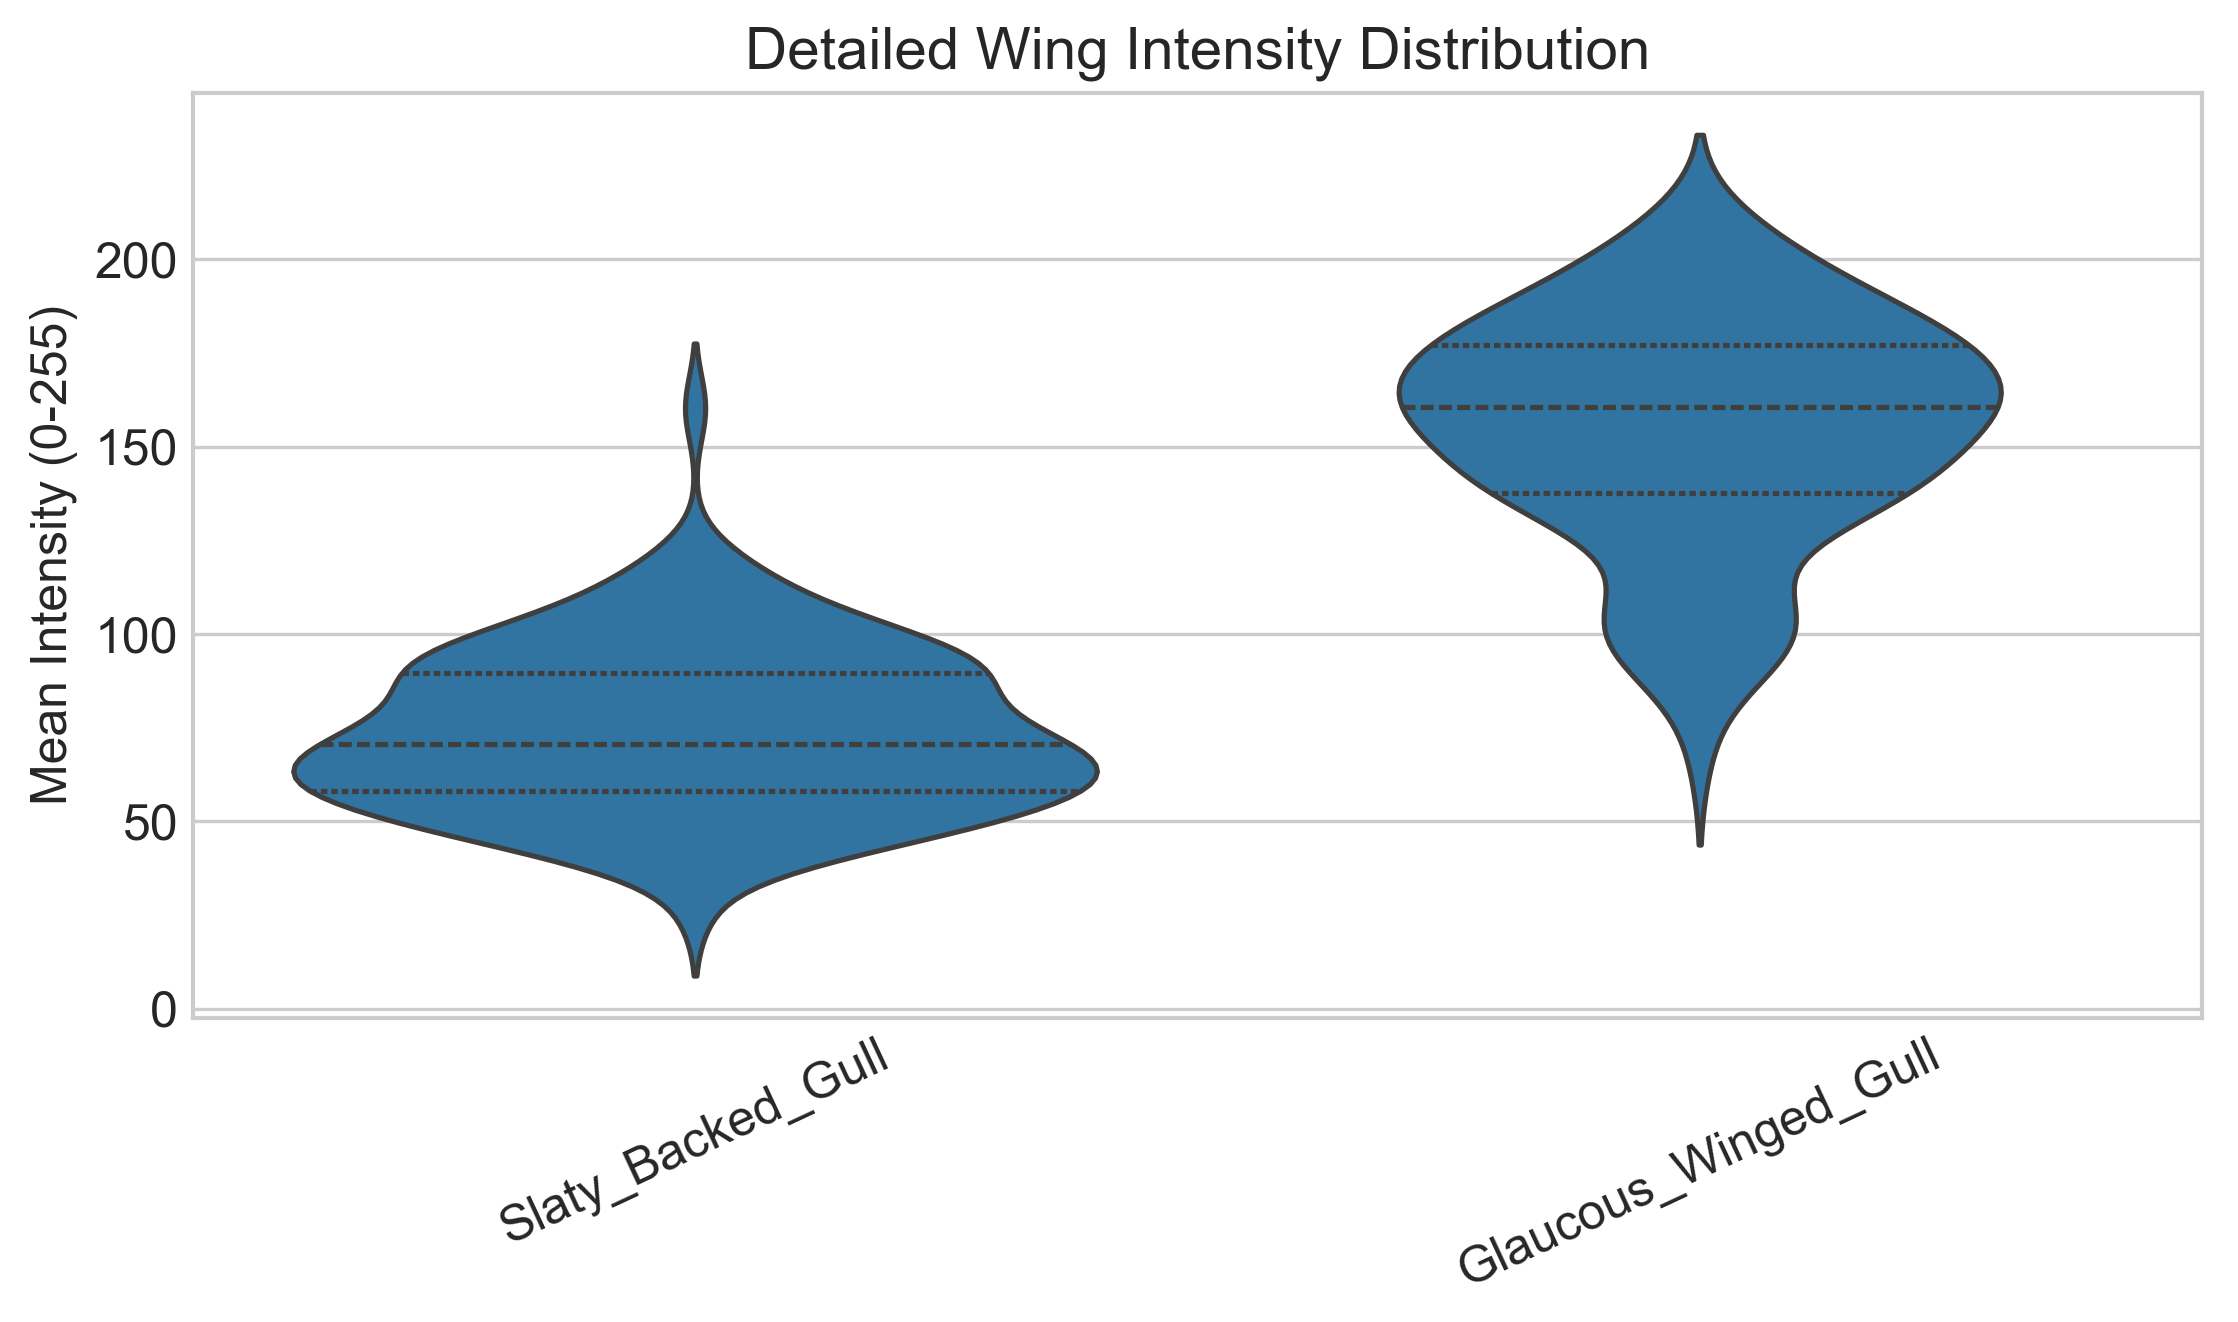
\includegraphics[width=\textwidth]{images/REPORT_IMAGES_INTENSITY/I2/wing_intensity_analysis.png}
%         \caption{Comparison of wing intensity values between species.}
%         \label{fig:wing_intensity}
%     \end{subfigure}
%     \hfill
%     \begin{subfigure}[b]{0.44\textwidth}
%         \centering
%         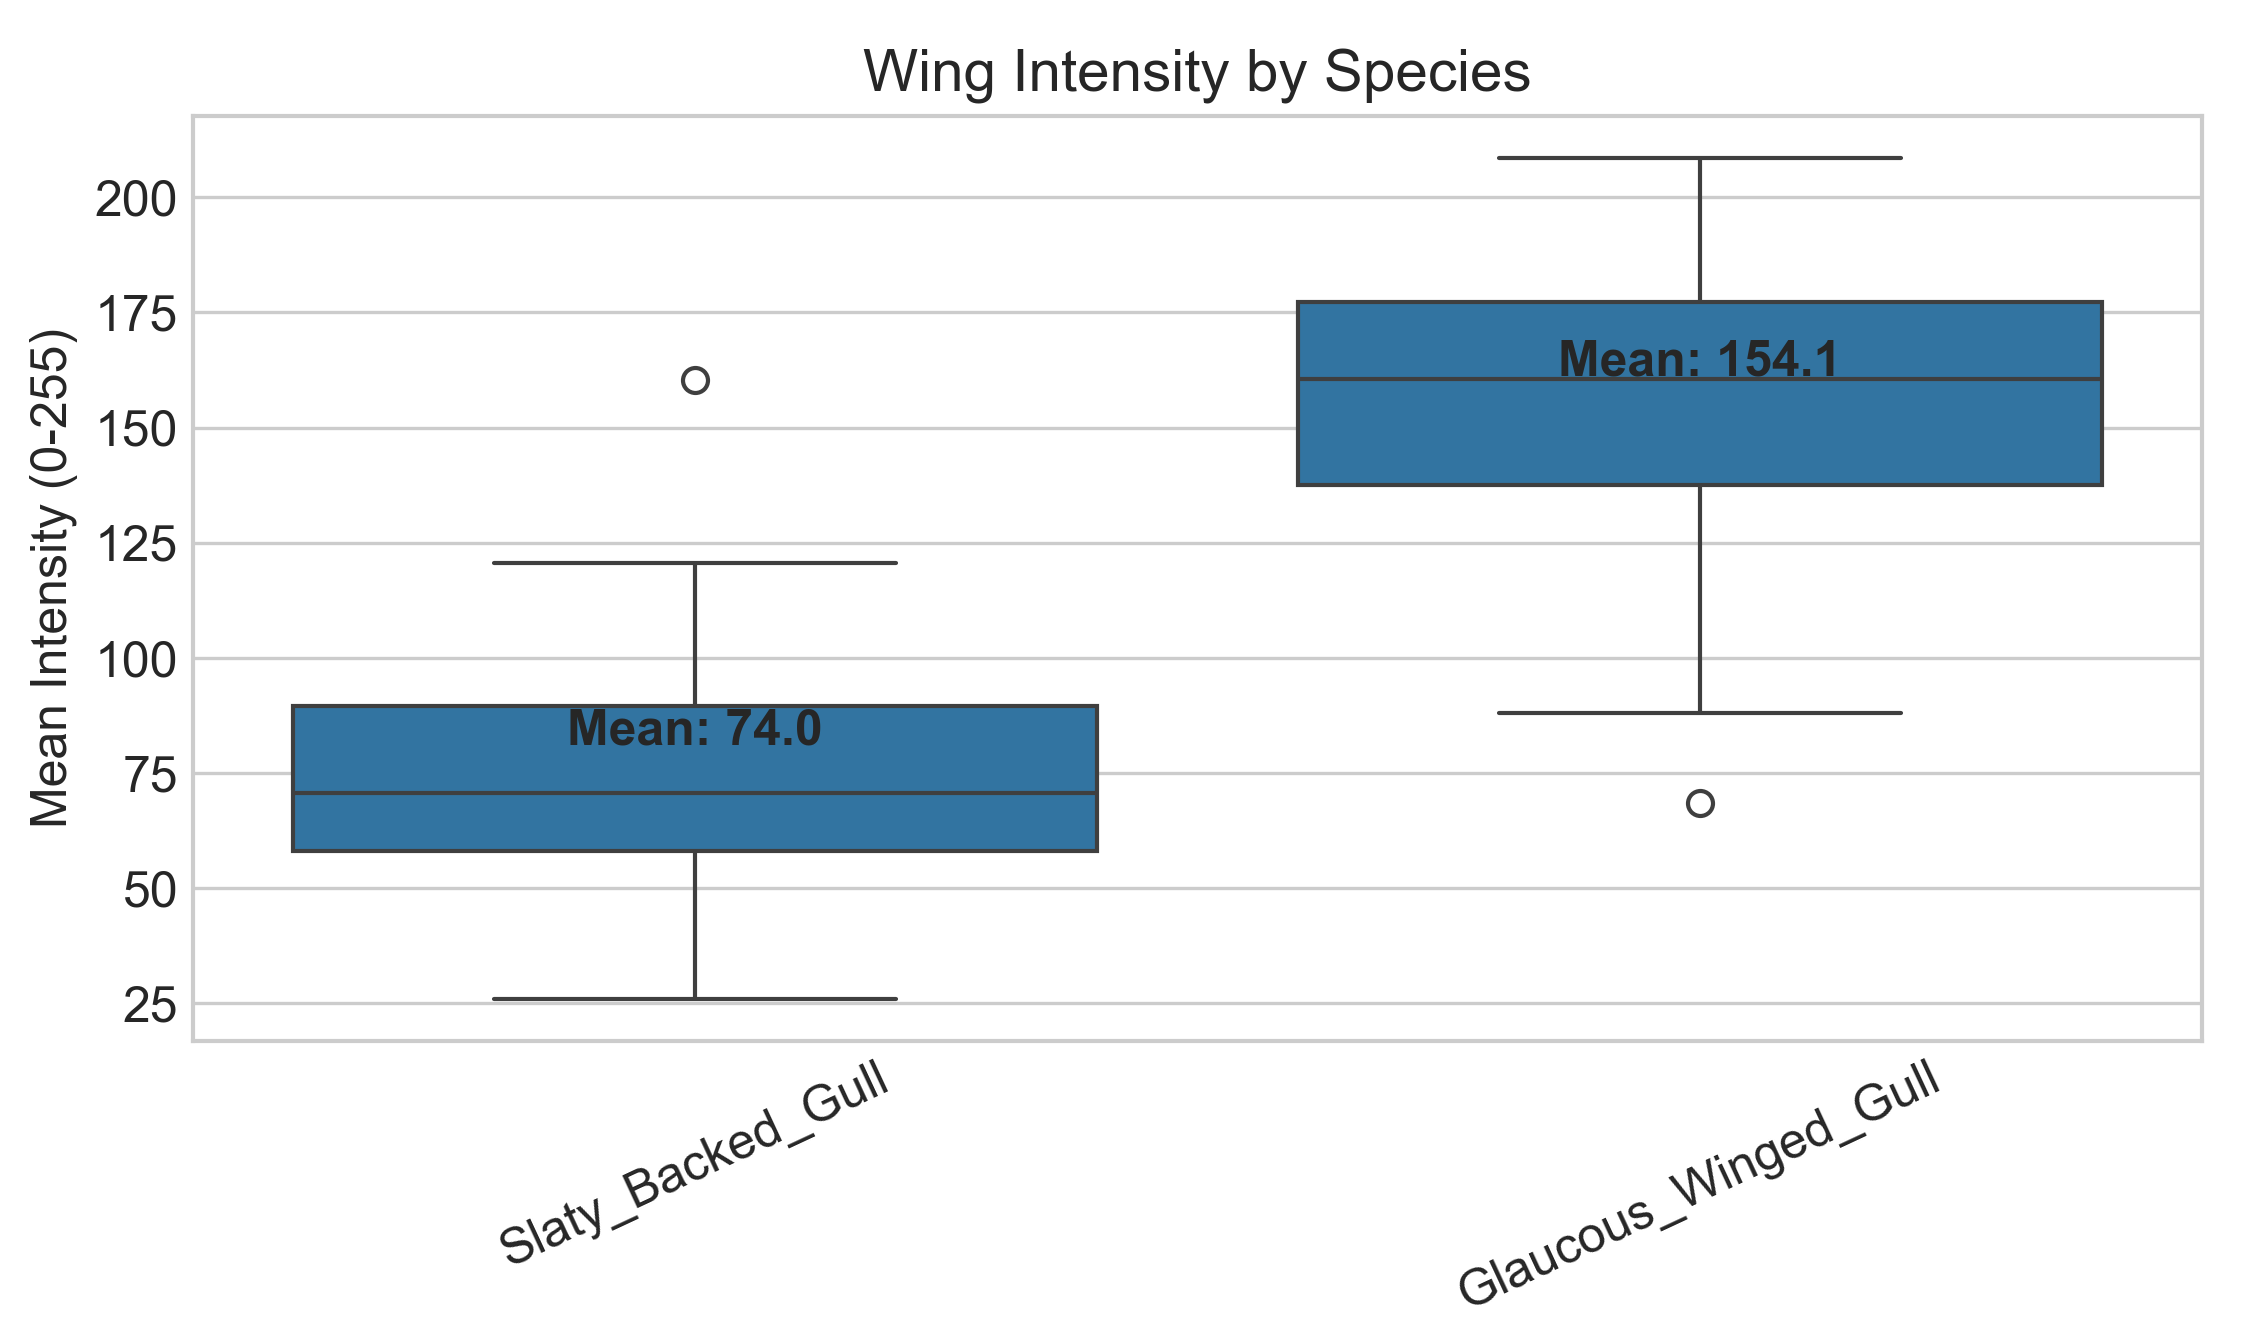
\includegraphics[width=\textwidth]{images/REPORT_IMAGES_INTENSITY/I2/WINGINTENSITY.png}
%         \caption{Mean wing intensity across samples.}
%         \label{fig:wing_intensity_means}
%     \end{subfigure}
%     % Vertical space between rows
%     \par\vspace{1.5ex}
%     % Second row
%     \begin{subfigure}[b]{0.44\textwidth}
%         \centering
%         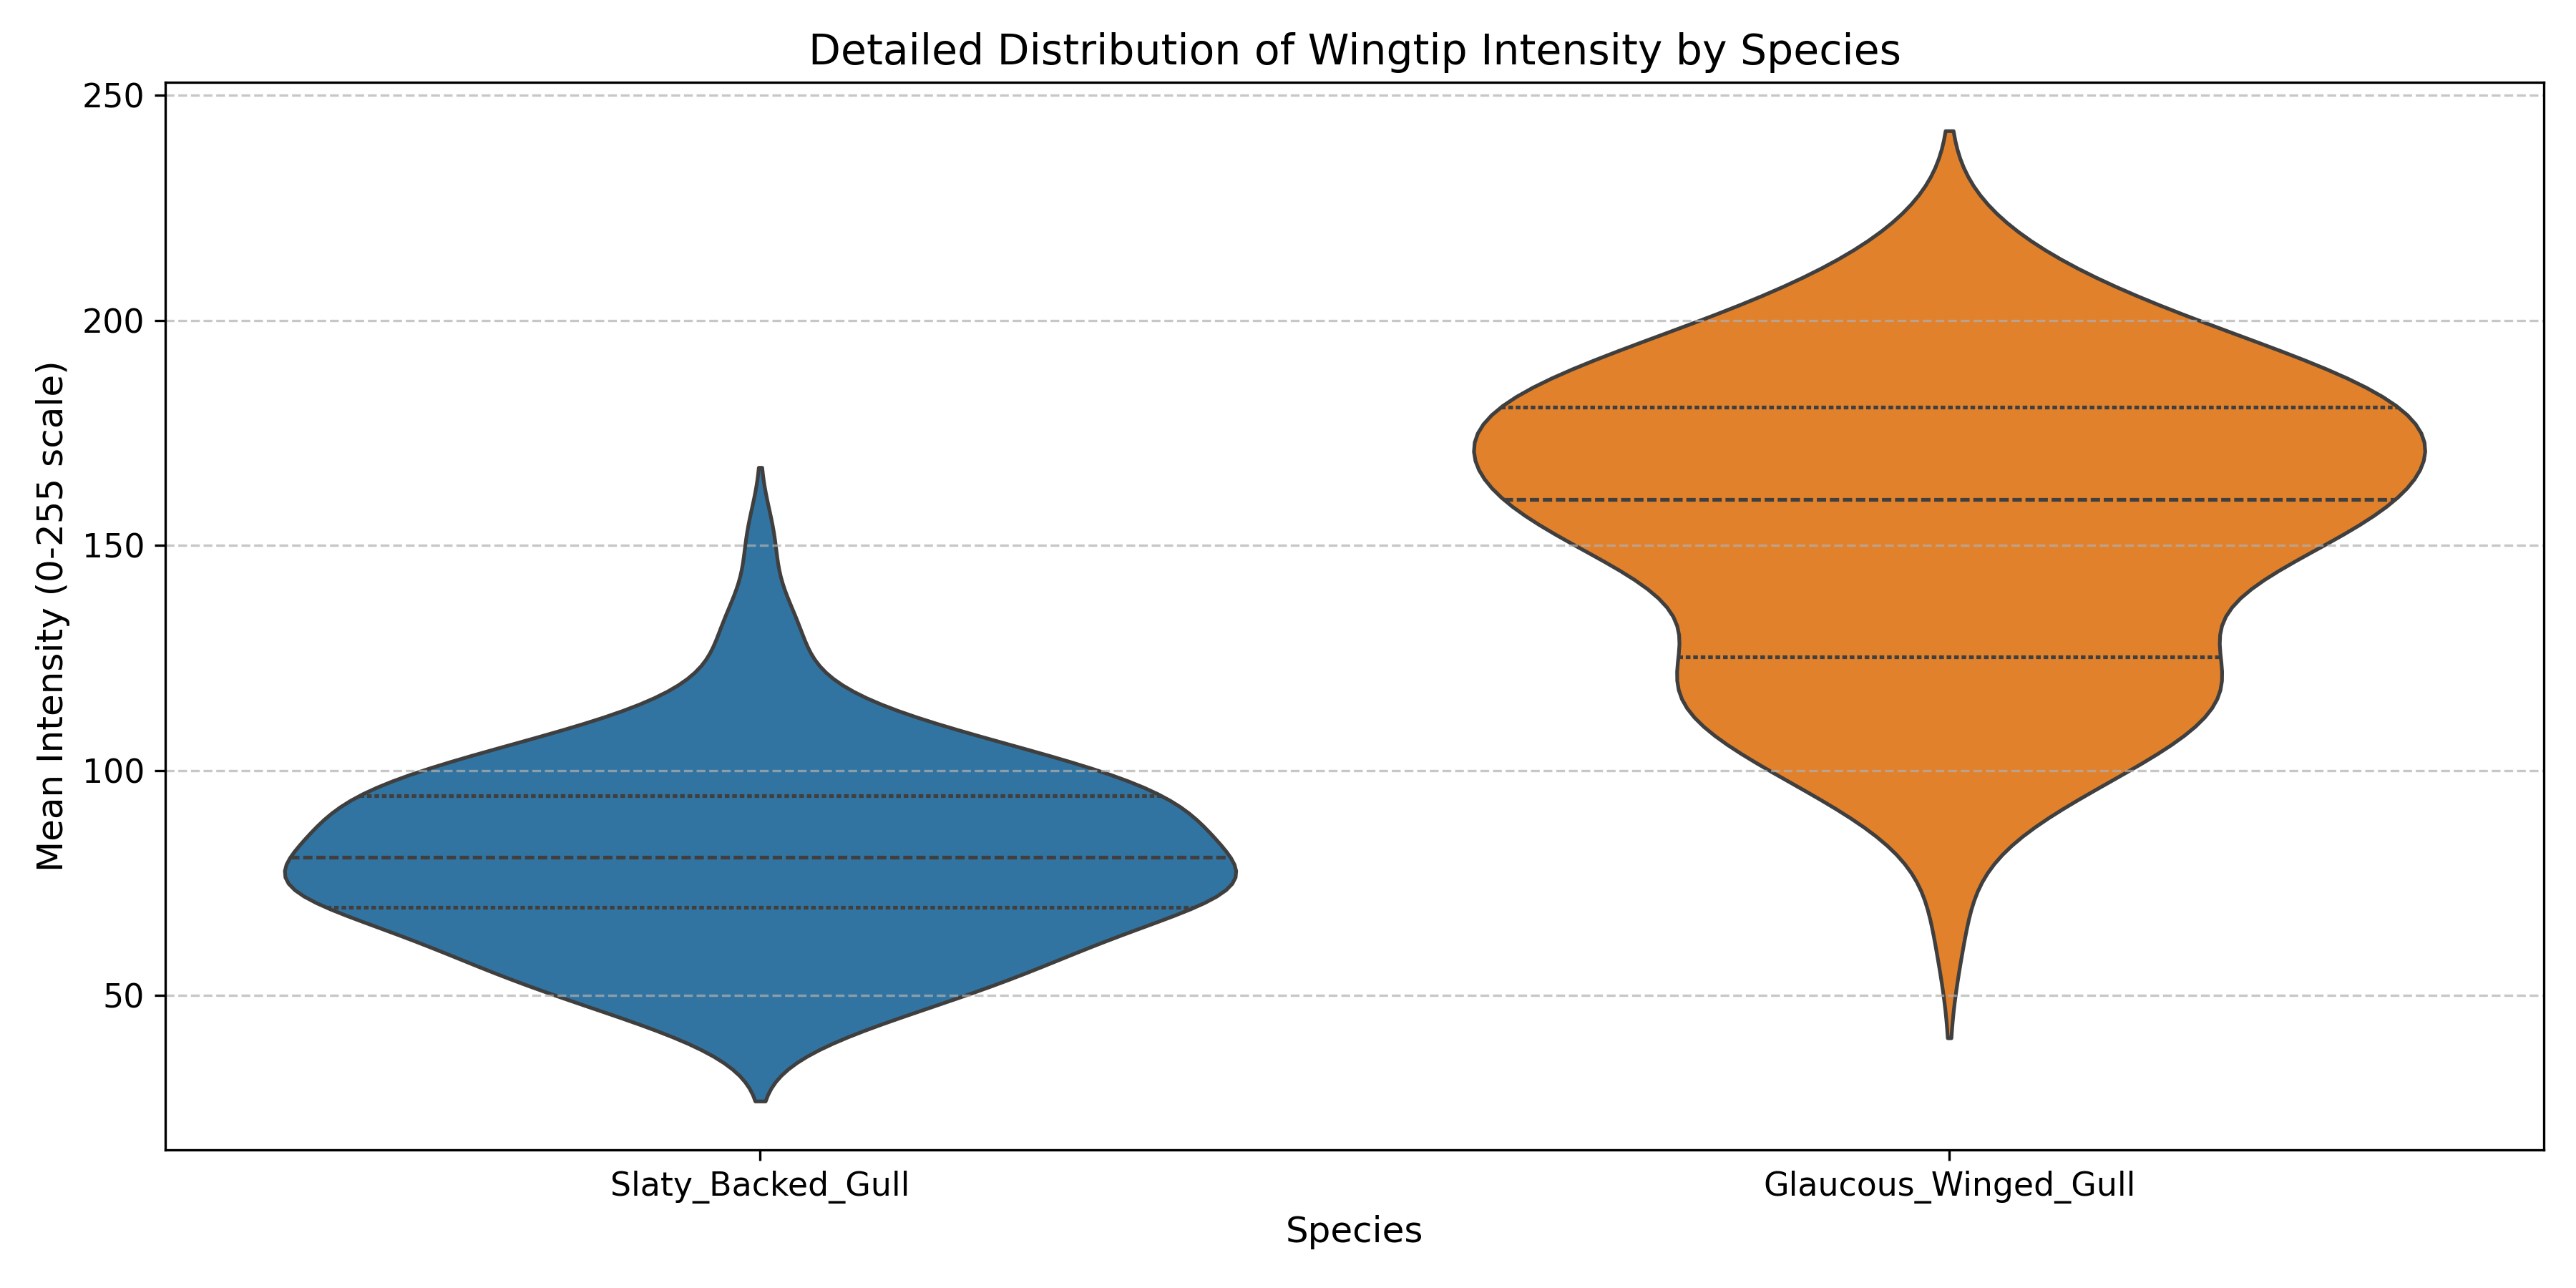
\includegraphics[width=\textwidth]{images/REPORT_IMAGES_INTENSITY/I2/wingtip_intensity_violin_plot.png}
%         \caption{Wingtip intensity violin plot.}
%         \label{fig:wingtip_intensity_violin}
%     \end{subfigure}
%     \hfill
%     \begin{subfigure}[b]{0.44\textwidth}
%         \centering
%         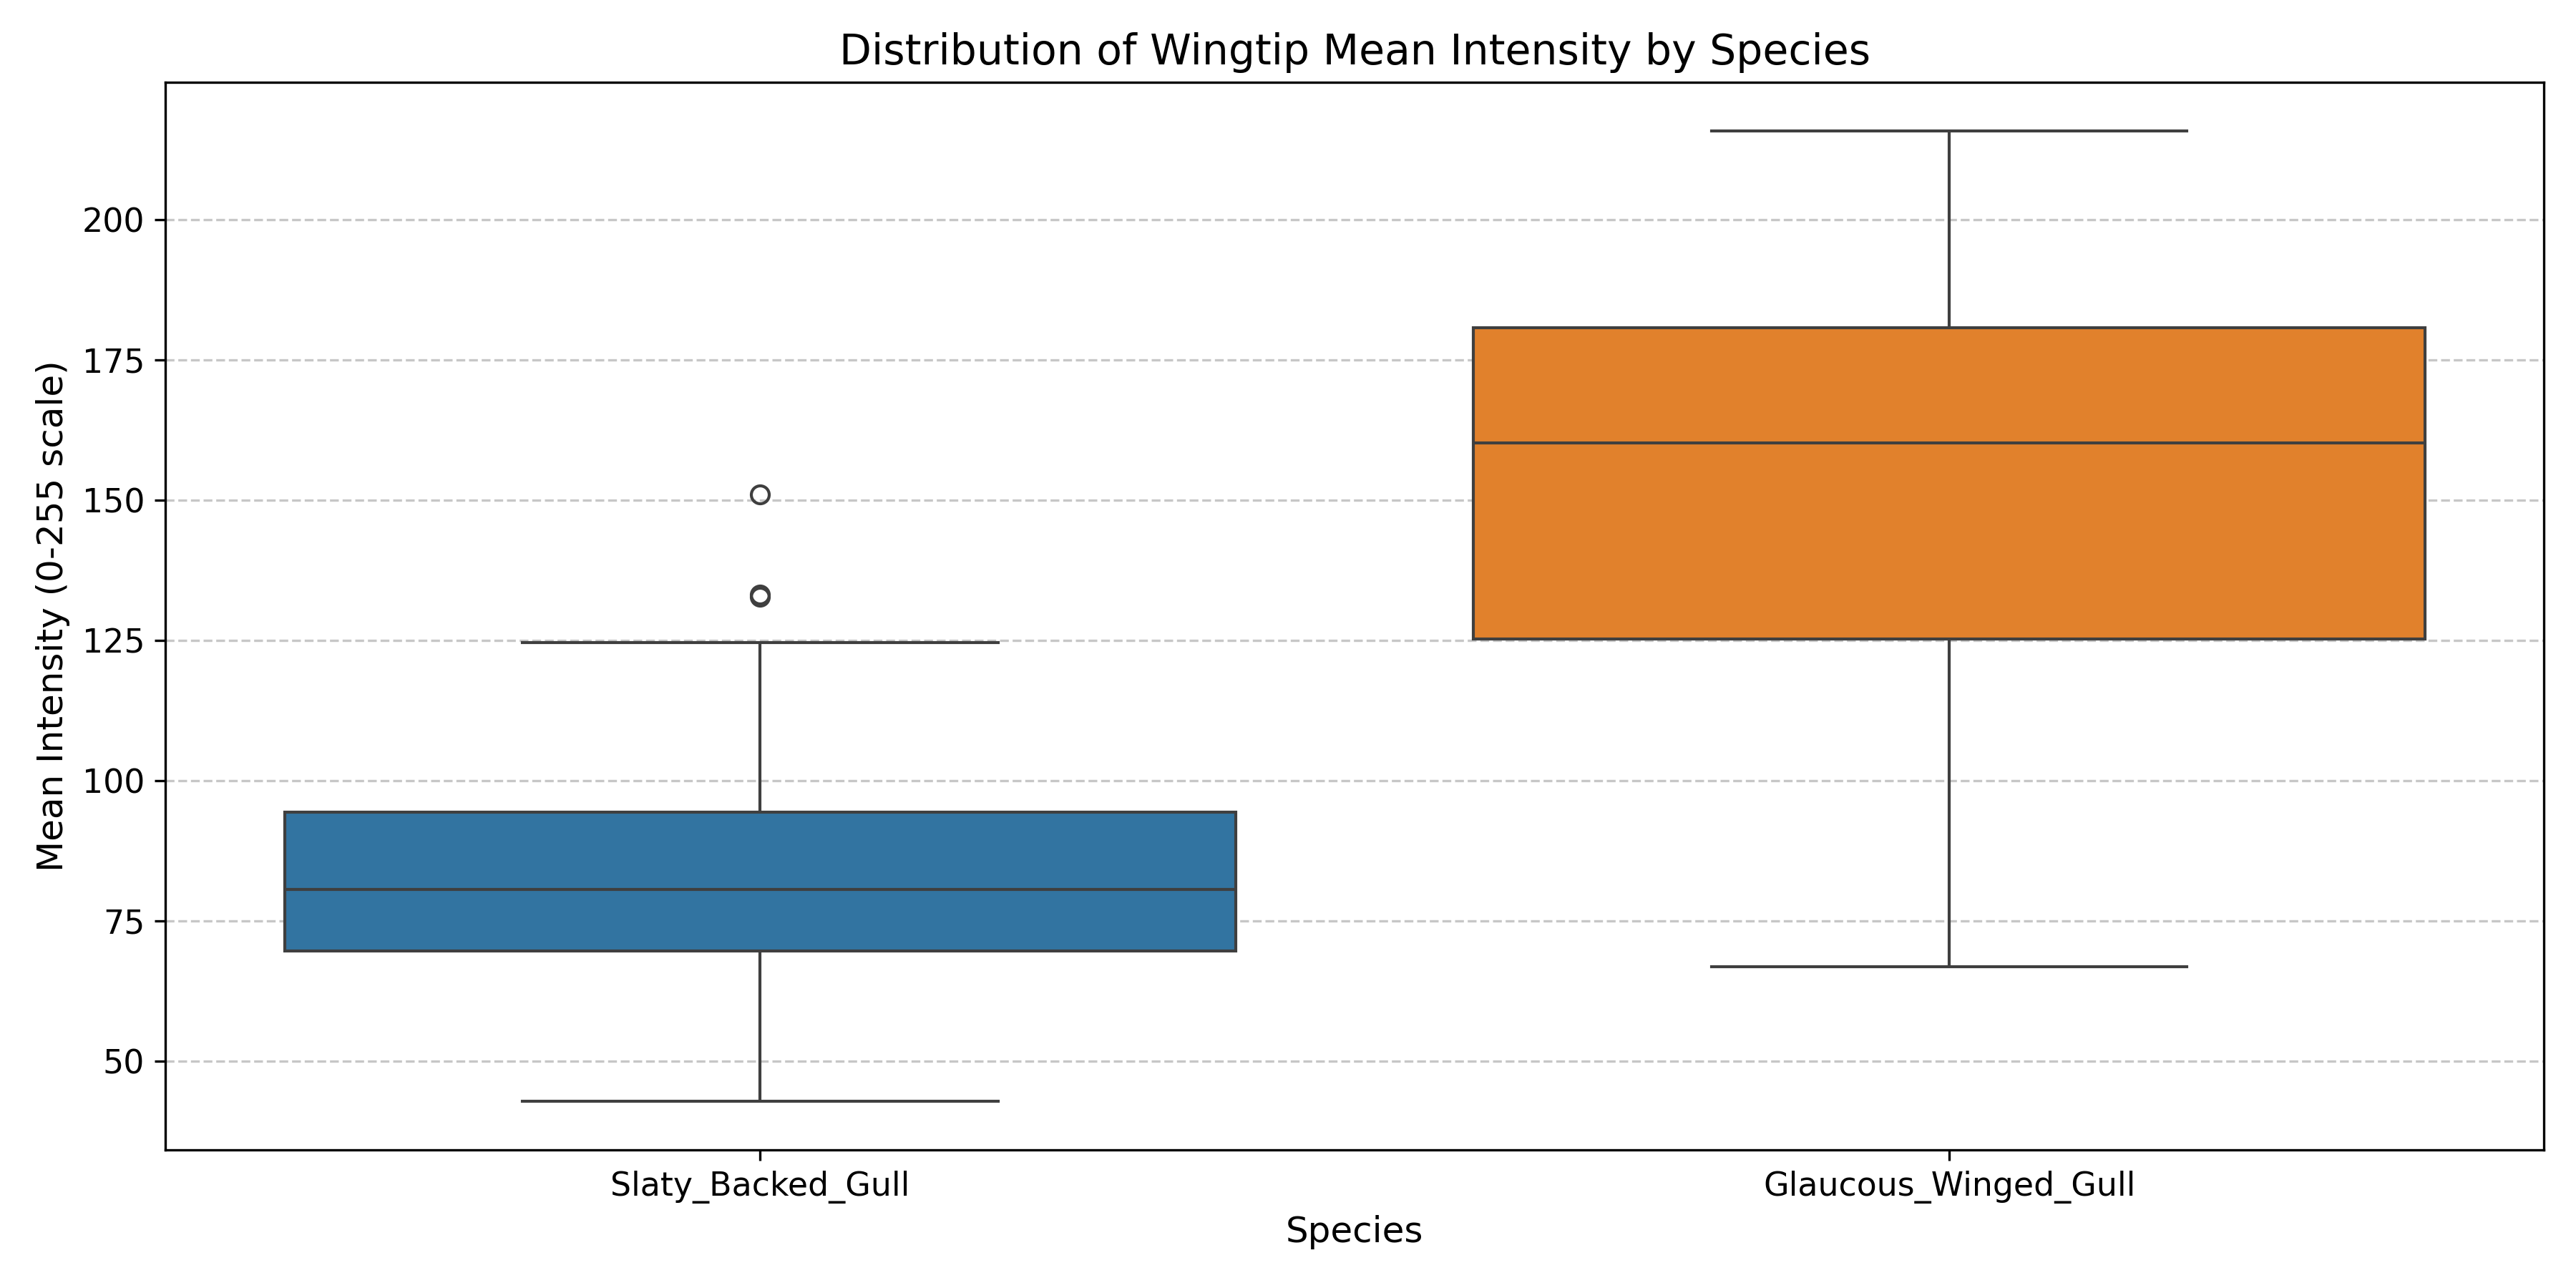
\includegraphics[width=\textwidth]{images/REPORT_IMAGES_INTENSITY/I2/wingtip_intensity_distribution.png}
%         \caption{Wingtip intensity distribution.}
%         \label{fig:wingtip_intensity_distribution}
%     \end{subfigure}
%     \caption{Wing and wingtip intensity metrics} %for Slaty-backed and Glaucous-winged Gulls, showing significant brightness differences.}
%     \label{fig:intensity_combined}
% \end{figure}

% The combined figure (\autoref{fig:intensity_combined}) summarizes the intensity analysis results. Subfigures~\ref{fig:wing_intensity} and~\ref{fig:wing_intensity_means} show that Glaucous-winged Gulls have consistently higher and less variable wing intensity than Slaty-backed Gulls. Subfigures~\ref{fig:wingtip_intensity_violin} and~\ref{fig:wingtip_intensity_distribution} illustrate that, while wingtip intensity also differs significantly between species, there is greater variability and overlap, as seen in the broader range and outliers in the distributions.
% While both wing and wingtip intensity are statistically significant distinguishing features, variations observed in the wingtip intensity distributions, potentially due to the presence of white spots and variations in darkness. For this reason the mean wing intensity may be considered a more consistently robust distinguishing feature between the two species.


\subsubsection{Wing Intensity}
Figures \ref{fig:wing_intensity} and \ref{fig:wing_intensity_means} show that Glaucous-winged Gulls have consistently higher and less variable wing intensity compared to Slaty-backed Gulls. The distributions are largely non-overlapping, making mean wing intensity a robust distinguishing feature between the species.

% Wing Intensity Figure
\begin{figure}[H]
    \centering
    \begin{subfigure}[b]{0.44\textwidth}
        \centering
        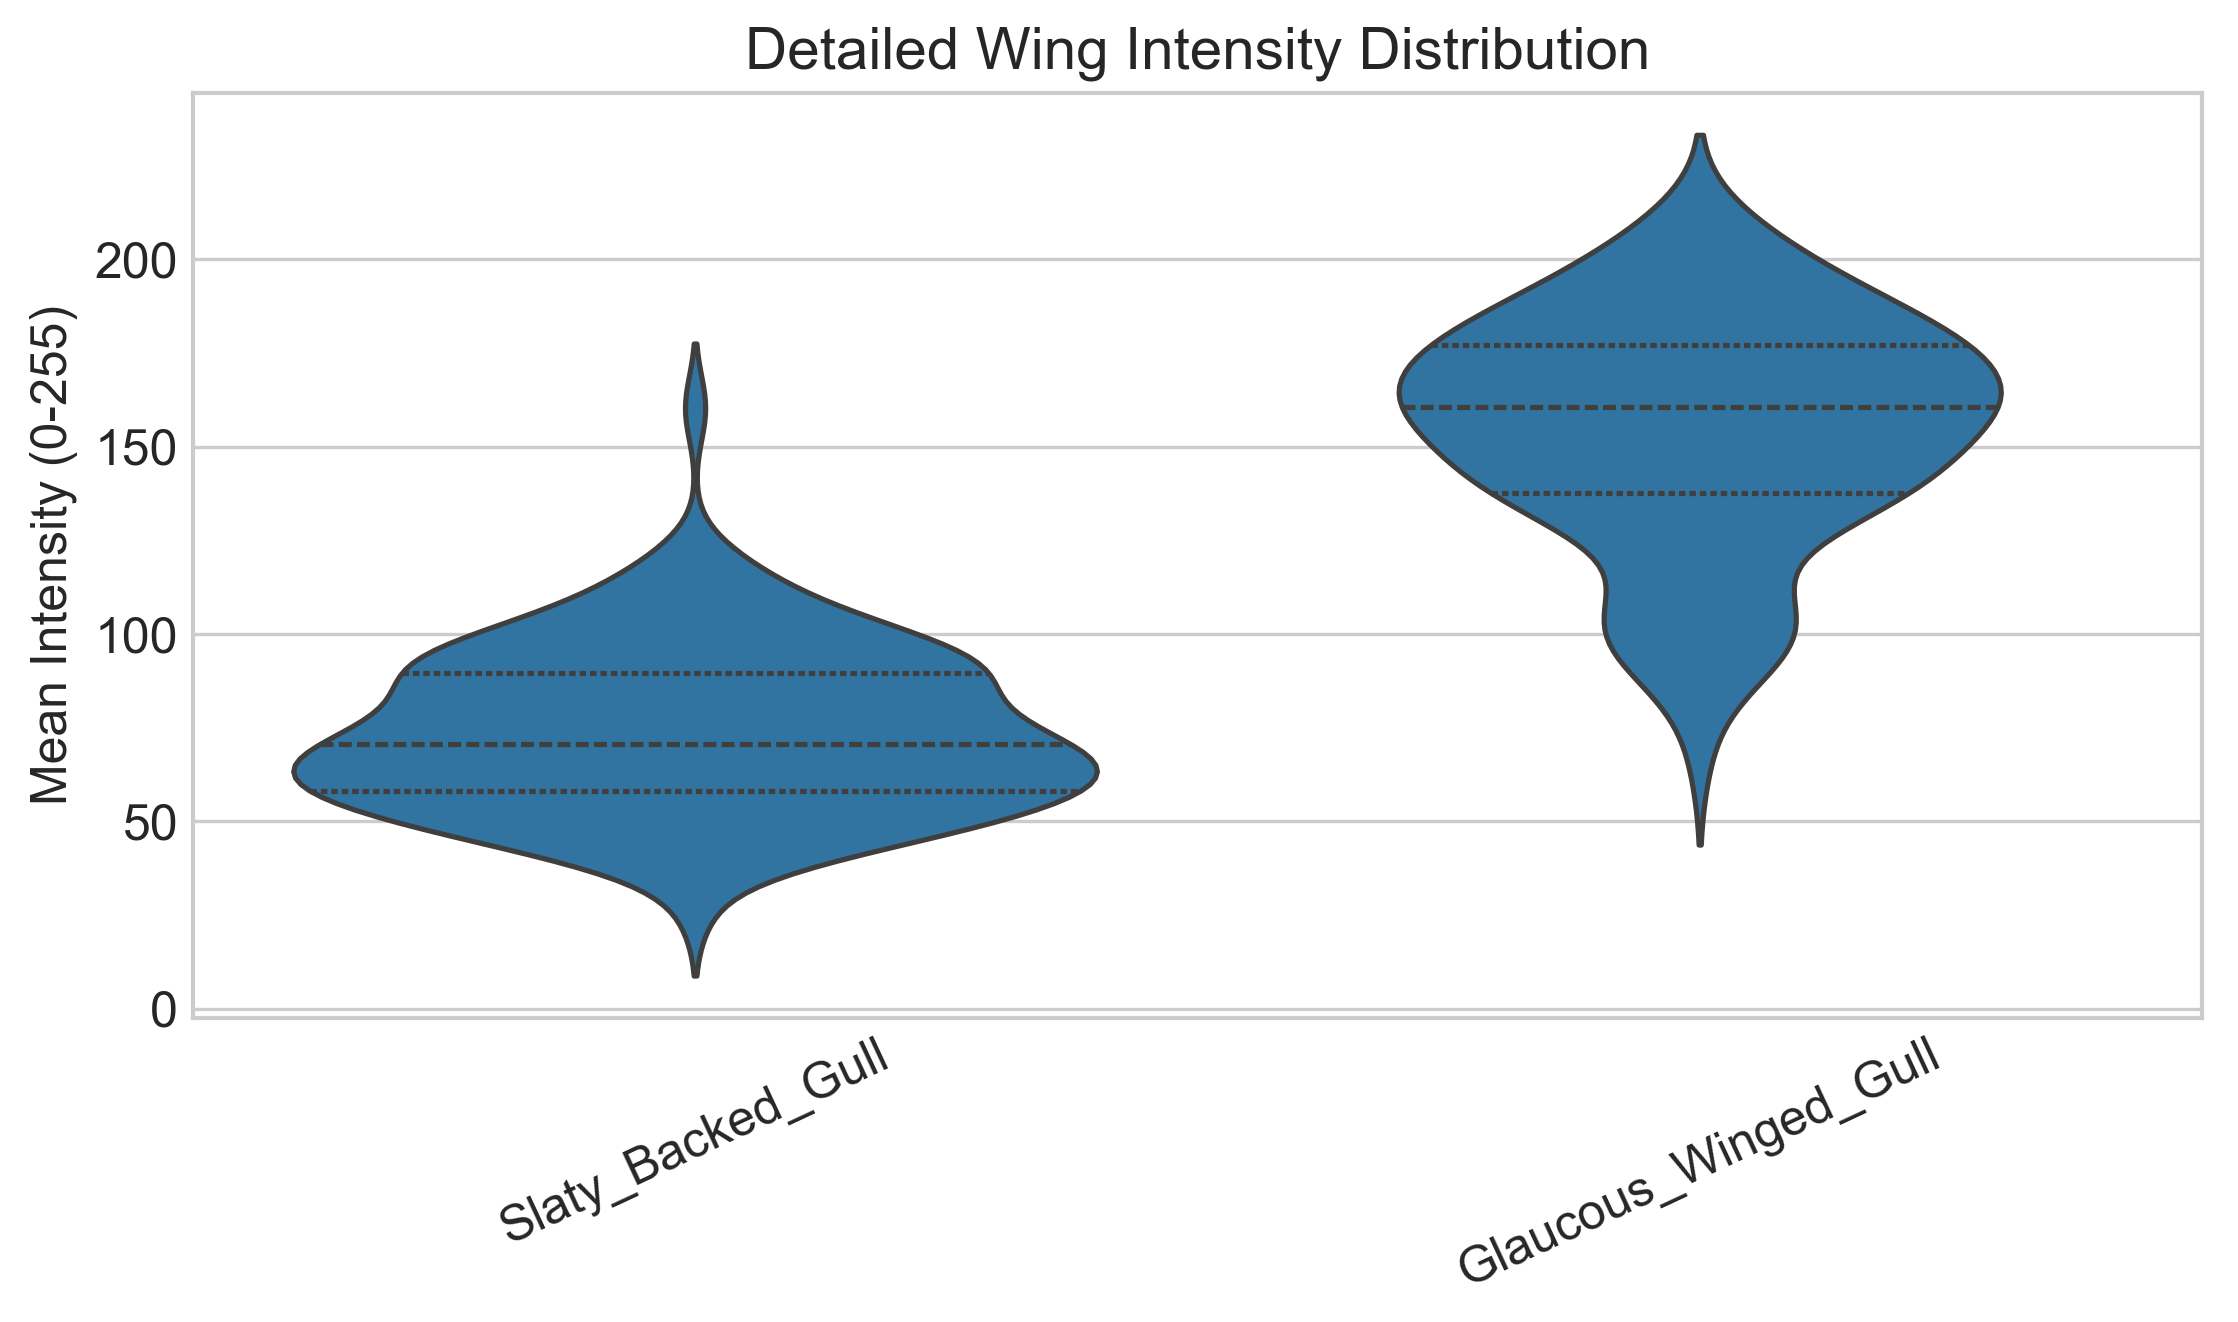
\includegraphics[width=\textwidth]{images/REPORT_IMAGES_INTENSITY/I2/wing_intensity_analysis.png}
        \caption{Comparison of wing intensity values between species.}
        \label{fig:wing_intensity}
    \end{subfigure}
    \hfill
    \begin{subfigure}[b]{0.44\textwidth}
        \centering
        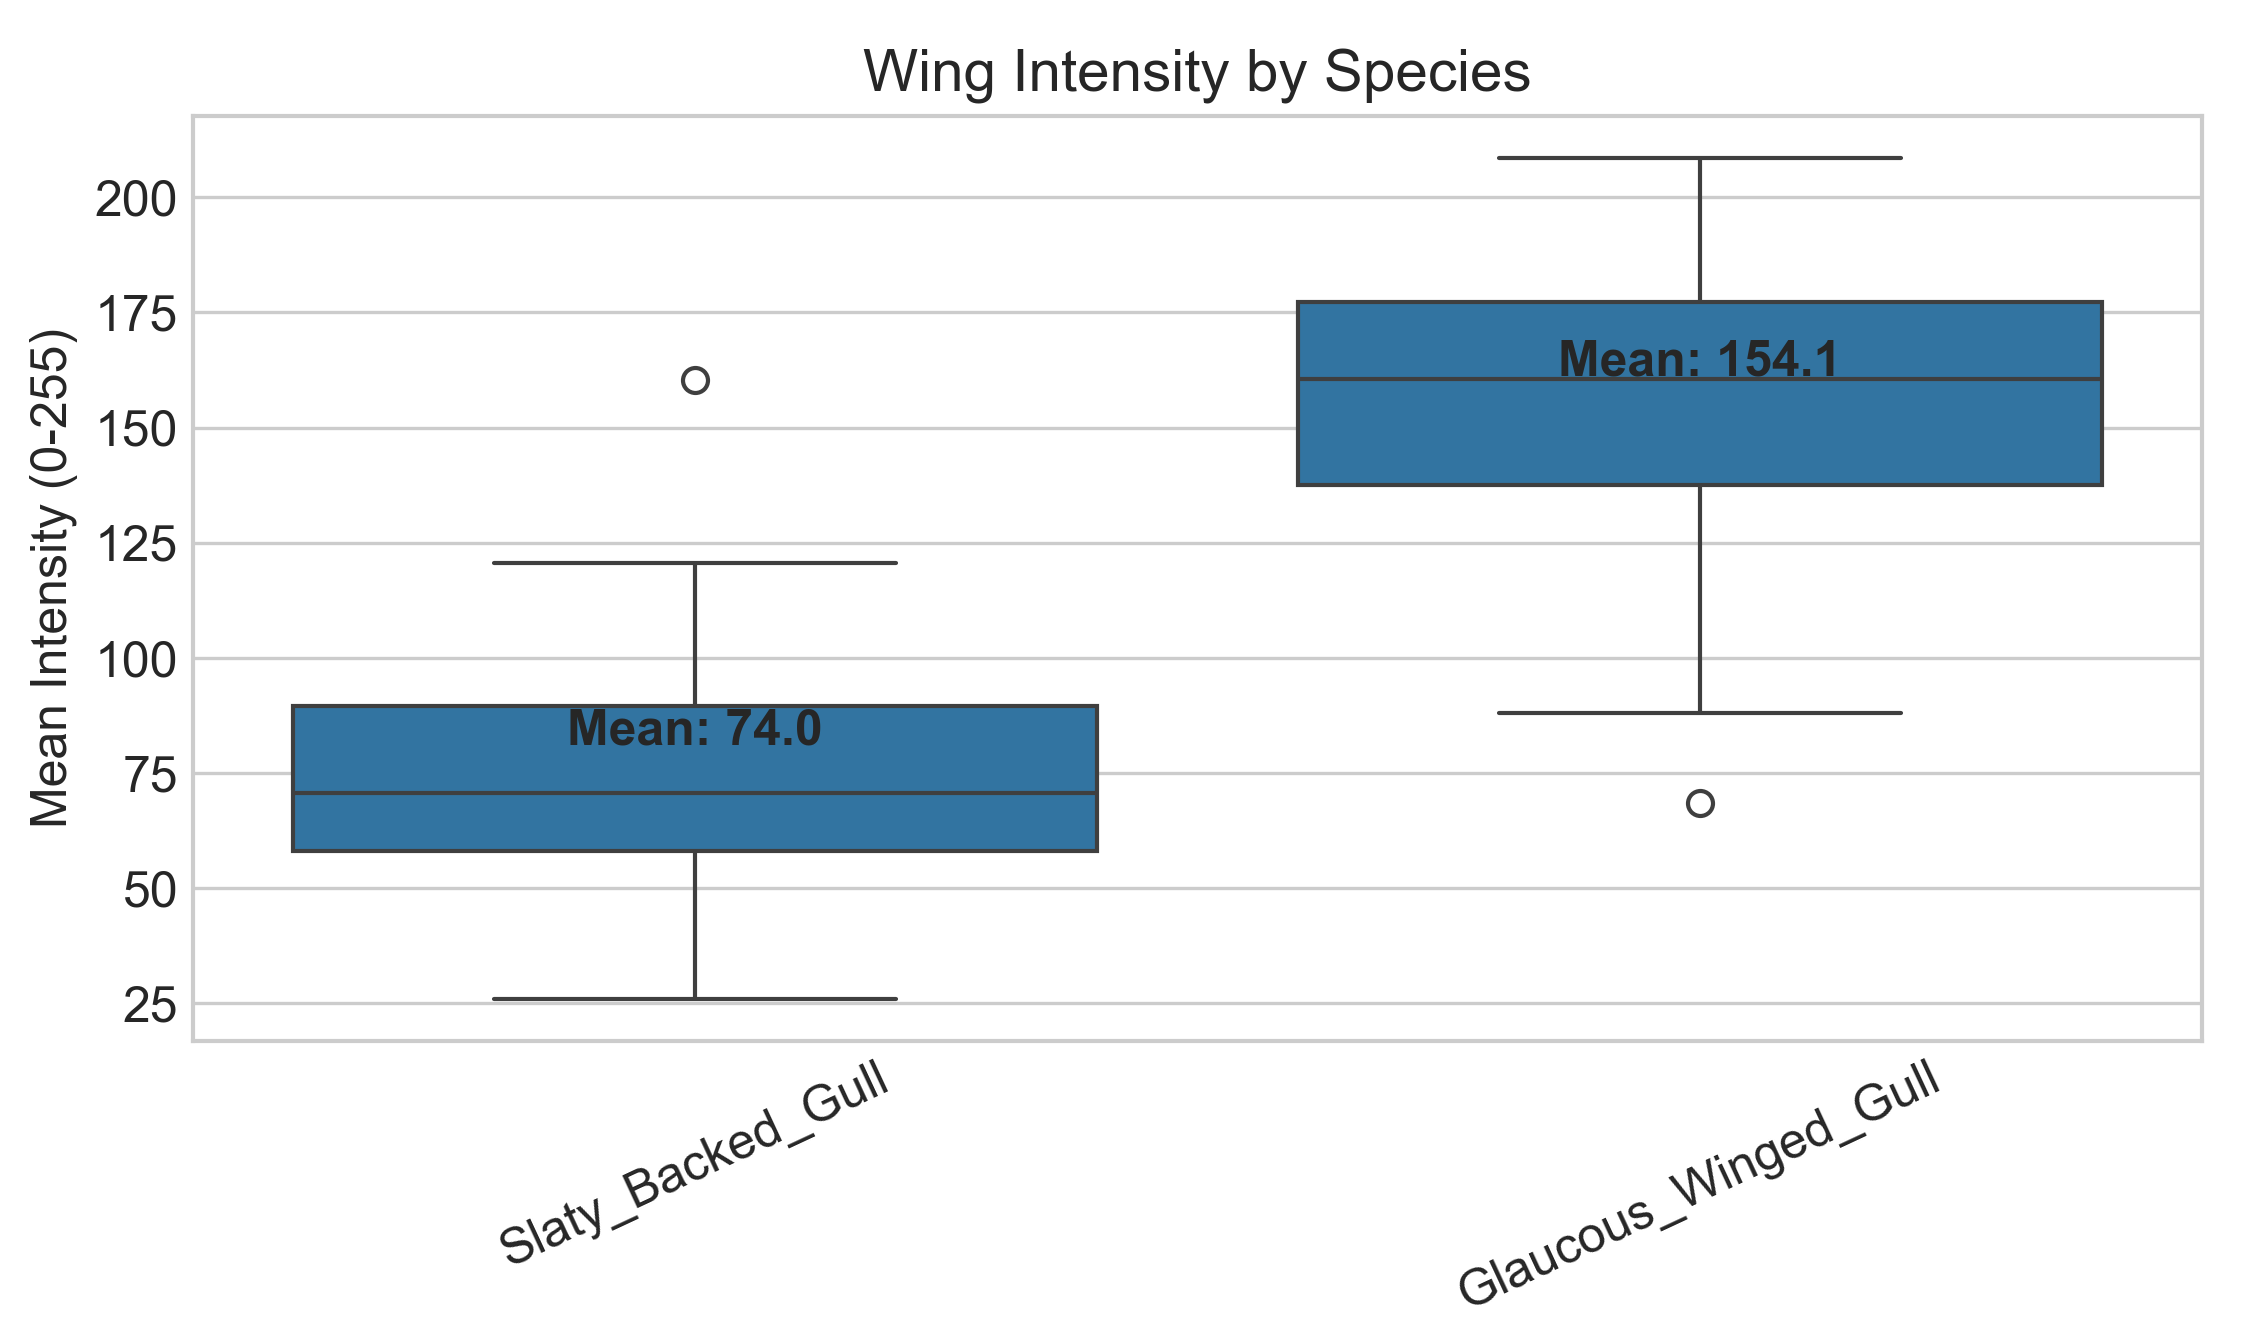
\includegraphics[width=\textwidth]{images/REPORT_IMAGES_INTENSITY/I2/WINGINTENSITY.png}
        \caption{Mean wing intensity across samples.}
        \label{fig:wing_intensity_means}
    \end{subfigure}
    \caption{Wing intensity metrics for Slaty-backed and Glaucous-winged Gulls, showing significant brightness differences.}
    \label{fig:wing_intensity_combined}
\end{figure}

\subsubsection{Wingtip Intensity}
Figures \ref{fig:wingtip_intensity_violin} and \ref{fig:wingtip_intensity_distribution} illustrate that, while wingtip intensity also differs significantly between species, there is greater variability and overlap, as indicated by the broader range and outliers. This variability is likely due to the presence of white spots and differences in darkness, making wingtip intensity less consistently robust than wing intensity for species differentiation.

% Wingtip Intensity Figure
\begin{figure}[H]
    \centering
    \begin{subfigure}[b]{0.44\textwidth}
        \centering
        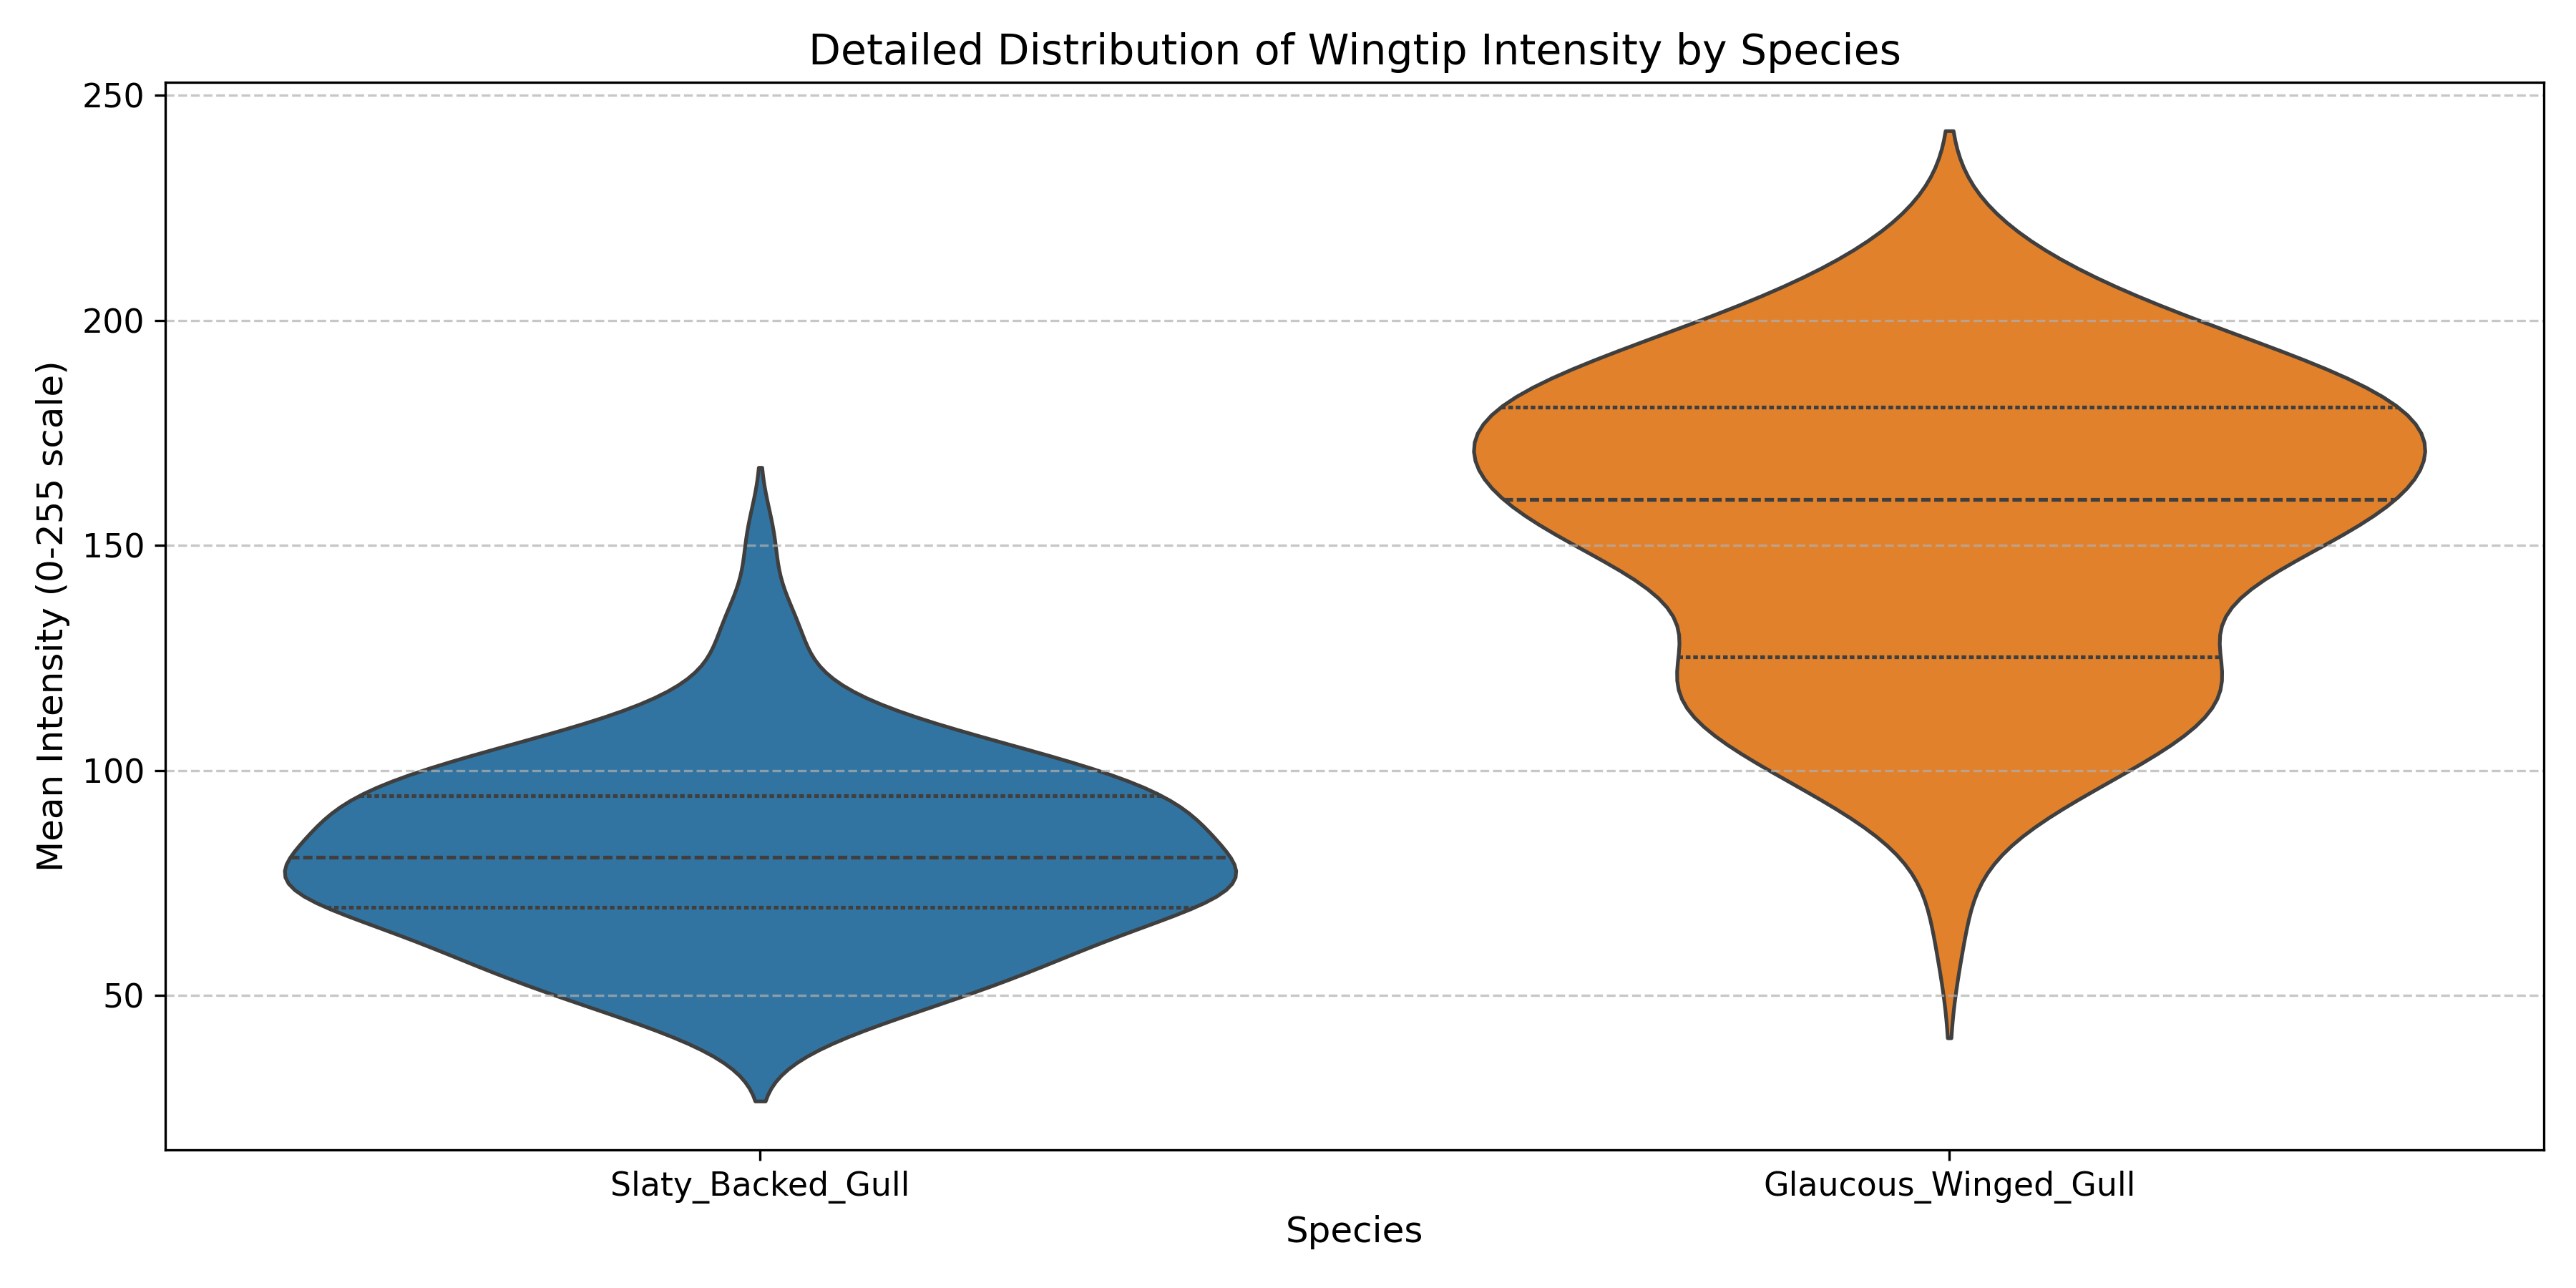
\includegraphics[width=\textwidth]{images/REPORT_IMAGES_INTENSITY/I2/wingtip_intensity_violin_plot.png}
        \caption{Wingtip intensity violin plot.}
        \label{fig:wingtip_intensity_violin}
    \end{subfigure}
    \hfill
    \begin{subfigure}[b]{0.44\textwidth}
        \centering
        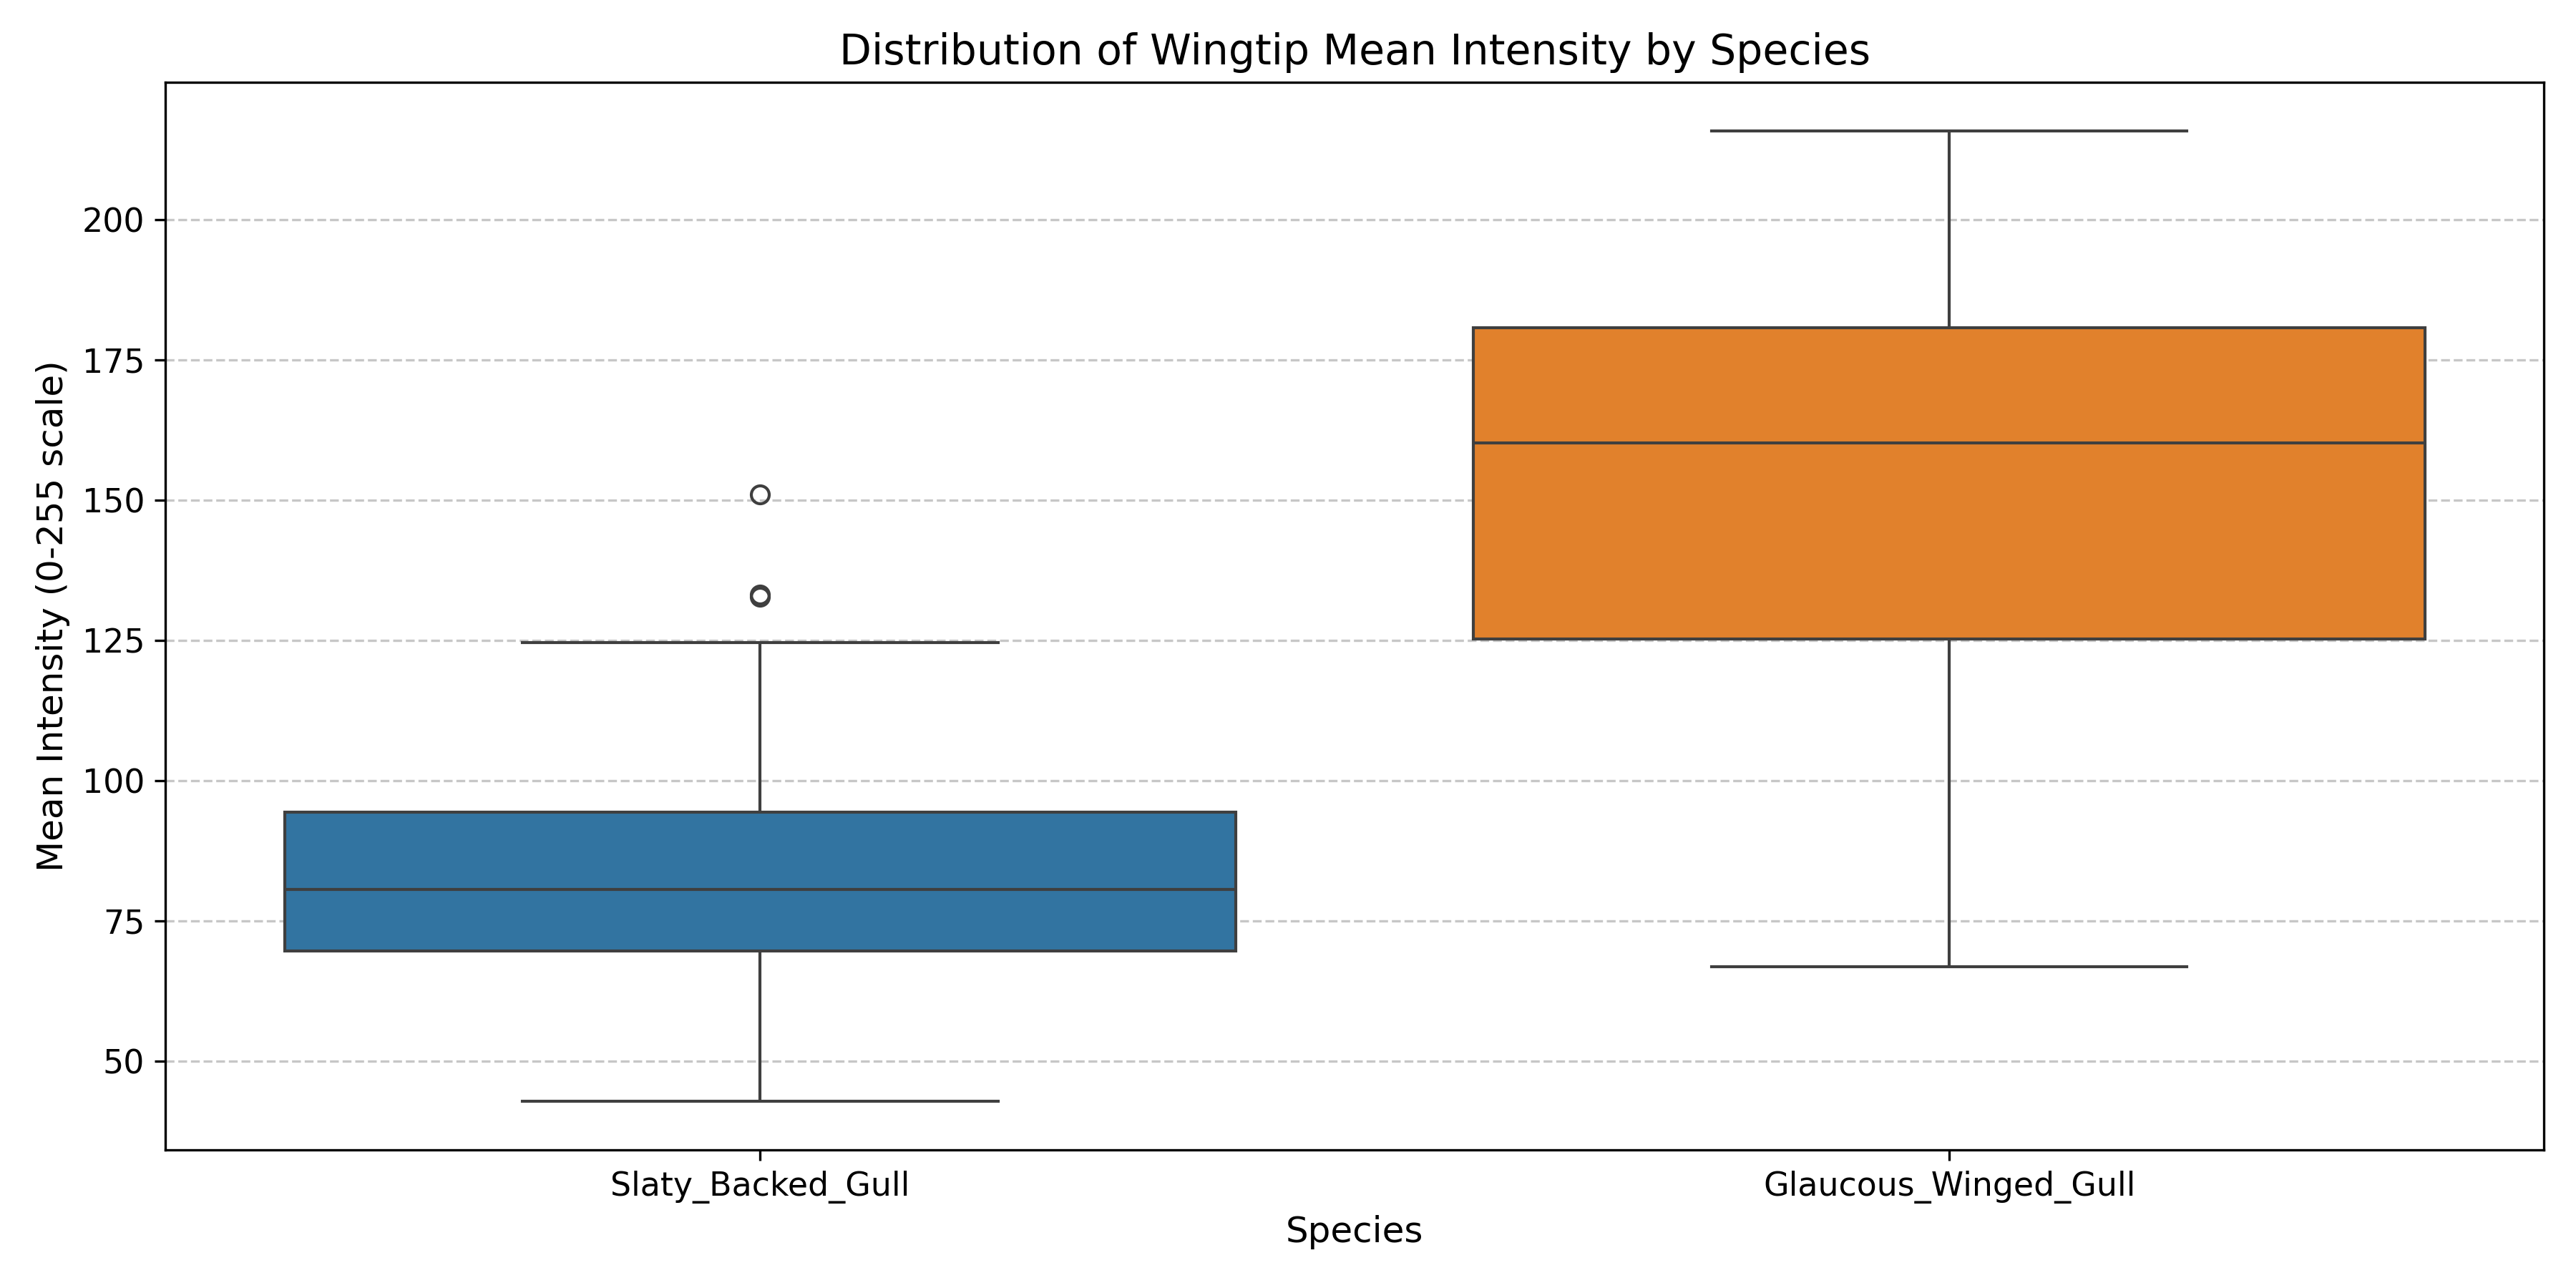
\includegraphics[width=\textwidth]{images/REPORT_IMAGES_INTENSITY/I2/wingtip_intensity_distribution.png}
        \caption{Wingtip intensity distribution.}
        \label{fig:wingtip_intensity_distribution}
    \end{subfigure}
    \caption{Wingtip intensity metrics for Slaty-backed and Glaucous-winged Gulls, highlighting greater variability and overlap between species.}
    \label{fig:wingtip_intensity_combined}
\end{figure}


\subsection{Distributions of Wing and Wingtip Intensities}

A comprehensive analysis of pixel intensity distributions in both the wing and wingtip regions reveals clear, species-specific patterns that distinguish Slaty-backed Gulls from Glaucous-winged Gulls. This section presents and interprets the observed distributions using multiple complementary metrics.

\subsection{Wing Intensity Distributions}

Figure~\ref{fig:wing_intensity_distribution} displays the distribution of mean wing intensities for both species. Slaty-backed Gulls cluster at lower mean intensity values, indicating darker wings, while Glaucous-winged Gulls are concentrated at higher mean intensities, reflecting lighter wings. The distributions are largely non-overlapping, underscoring a strong differentiation in overall wing brightness between the two species.

\begin{figure}[H]
    \centering
    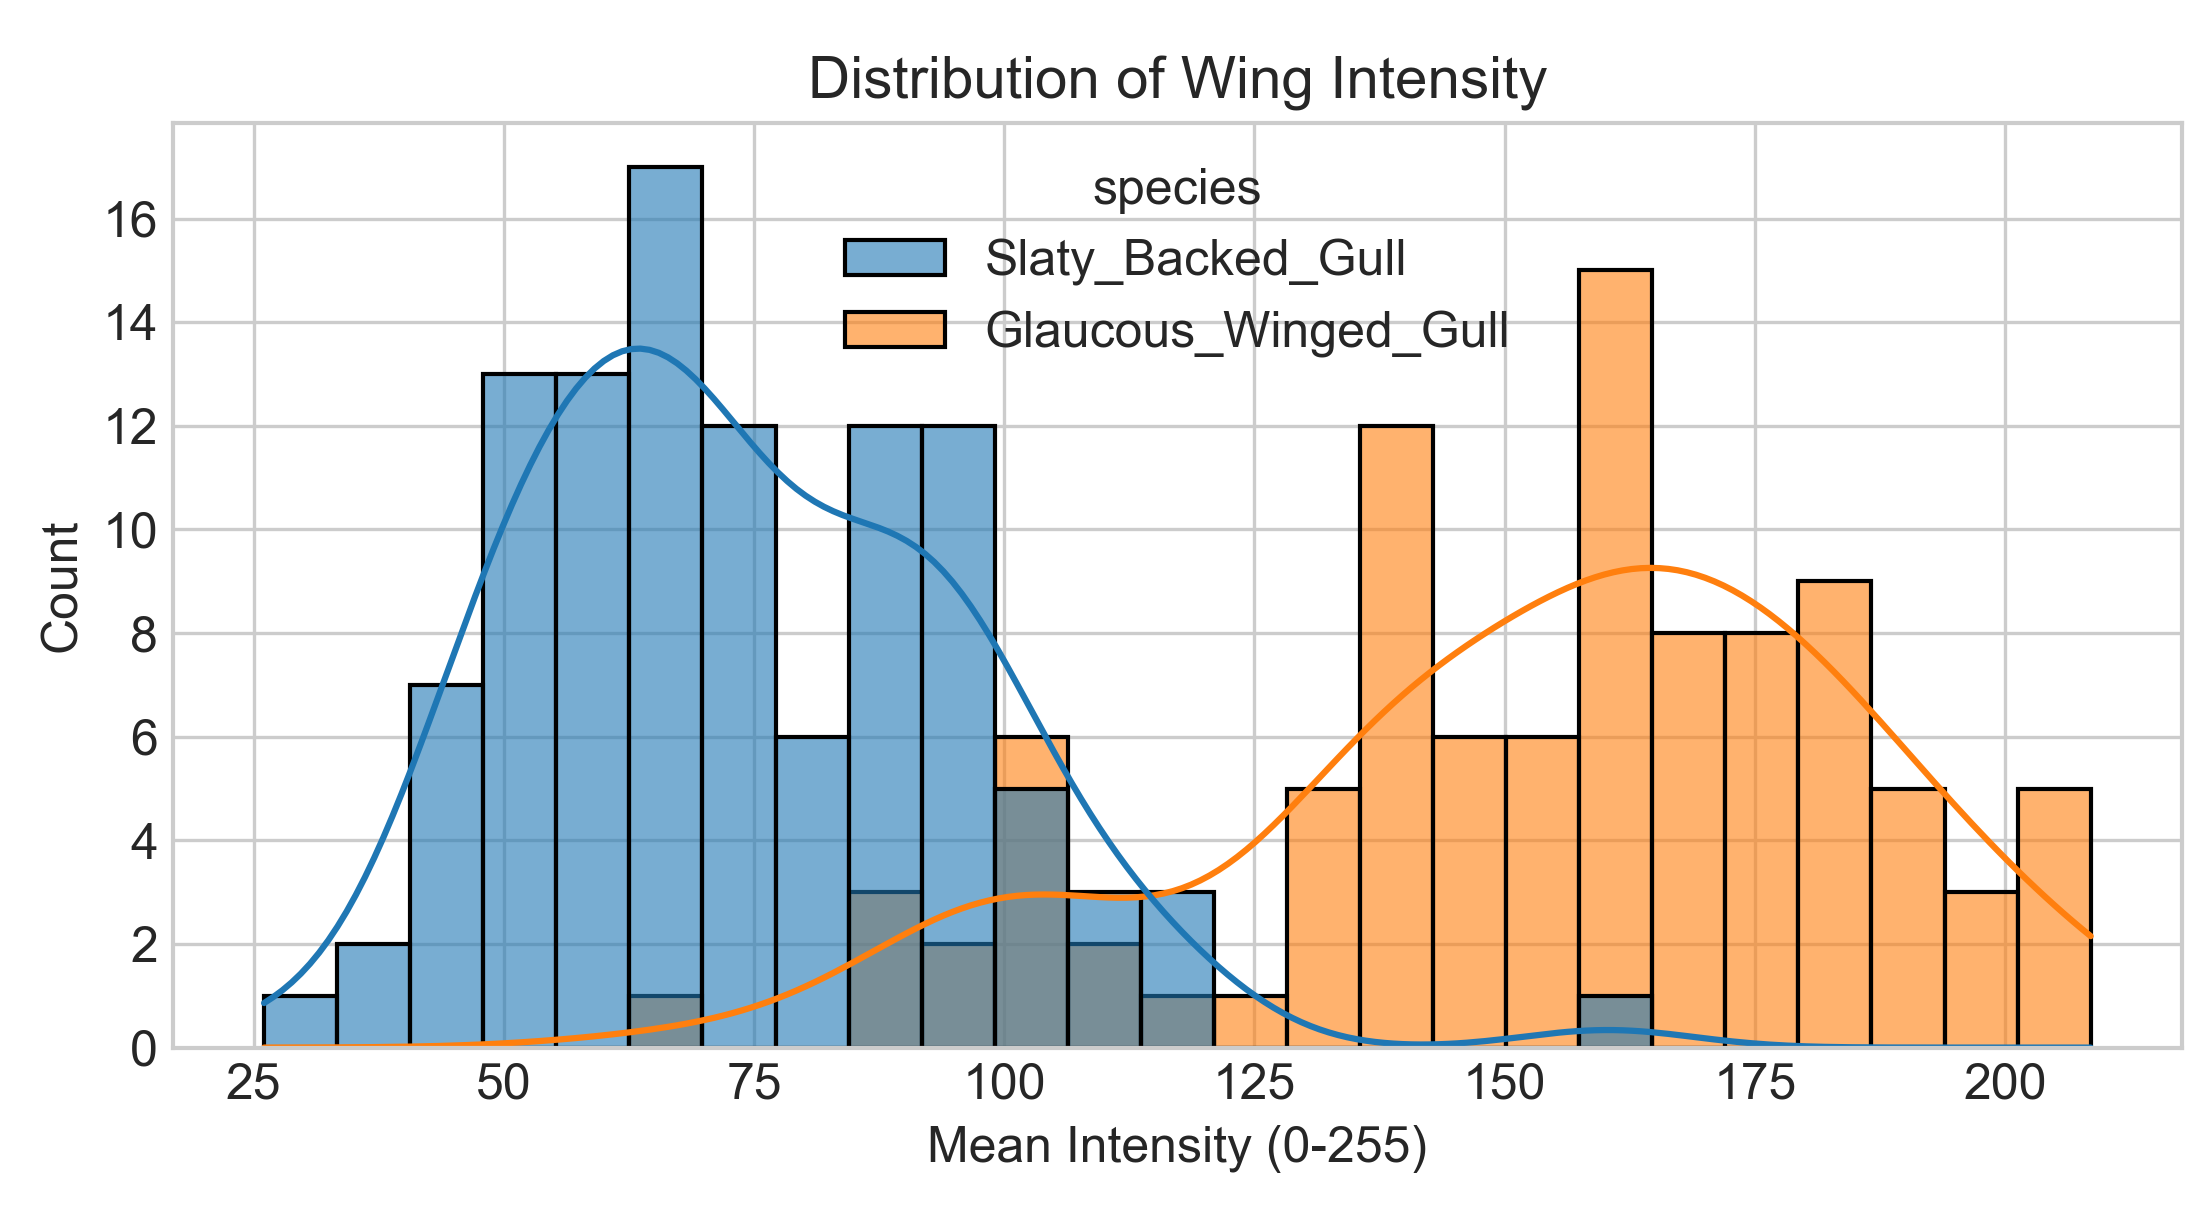
\includegraphics[width=0.55\textwidth]{images/REPORT_IMAGES_INTENSITY/I2/distribution.png}
    \caption{Distribution of mean wing intensity for Slaty-backed Gulls (blue) and Glaucous-winged Gulls (orange). Each species forms a distinct cluster, reflecting their characteristic wing brightness.}
    \label{fig:wing_intensity_distribution}
\end{figure}


\subsection{Wingtip Intensity Distributions}

The distributions of wingtip pixel intensities for both species are shown in Figure~\ref{fig:wingtip_intensity_distributions}. Slaty-backed Gulls (orange) have a higher proportion of darker pixels (lower intensity values), while Glaucous-winged Gulls (blue) show a greater proportion of lighter pixels (higher intensity values). Both grouped and fine-grained binning approaches reveal unique, largely non-overlapping patterns for each species.

\begin{figure}[H]
    \centering
    \begin{subfigure}[b]{0.47\textwidth}
        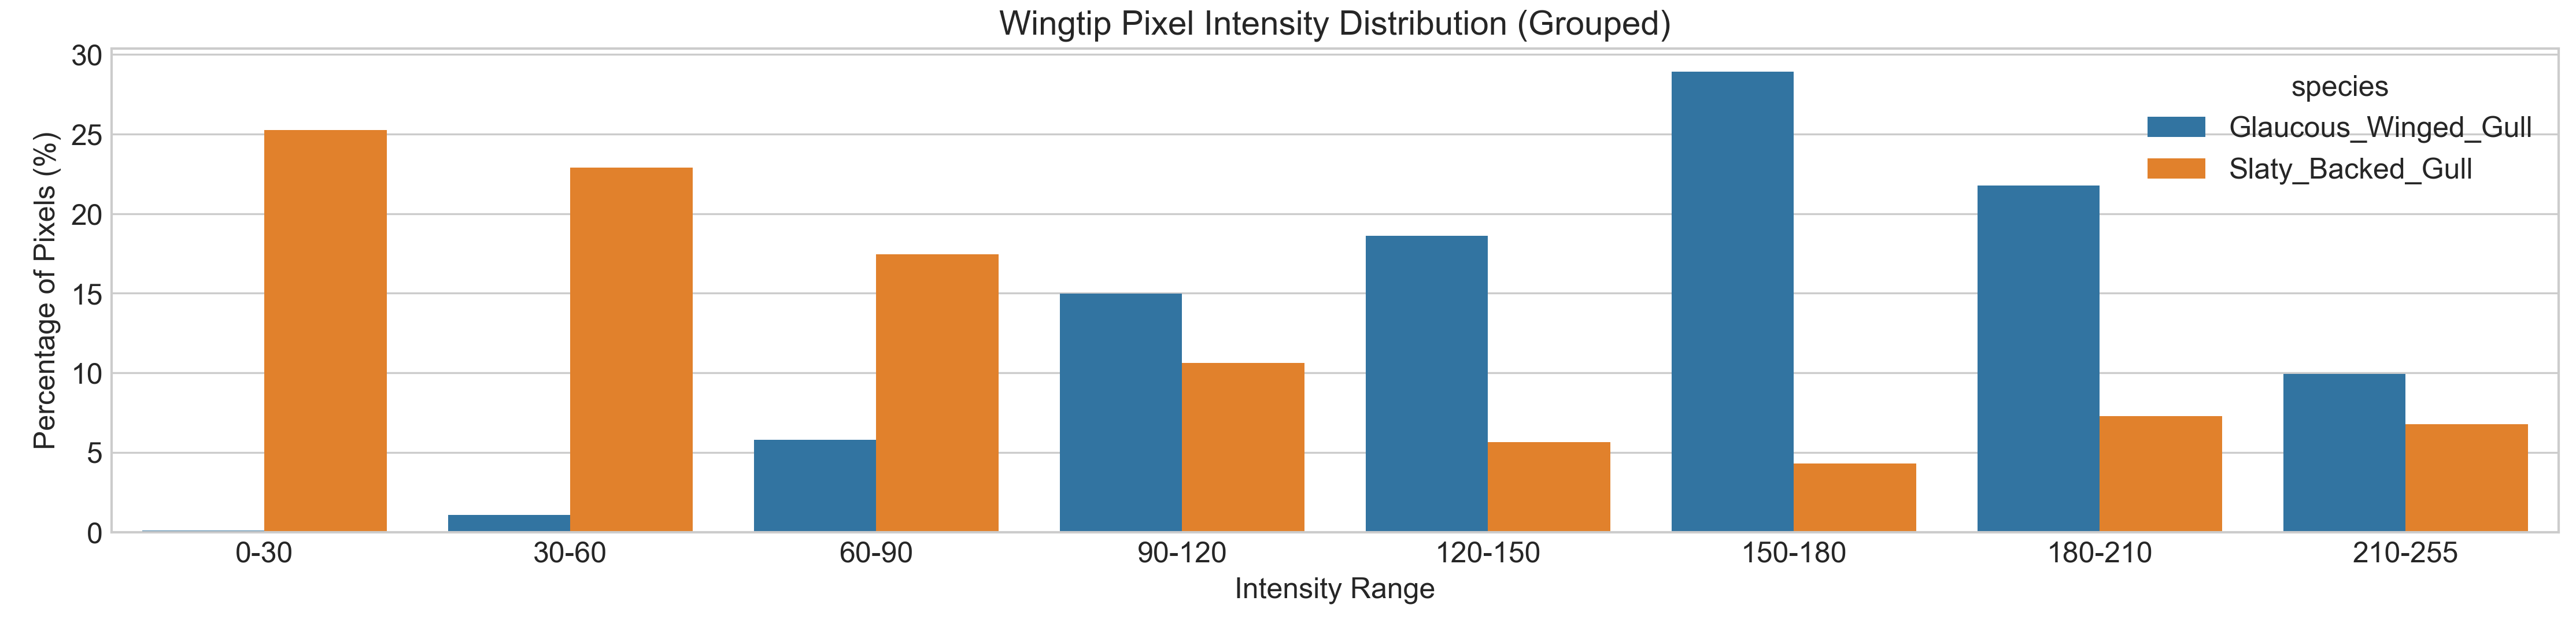
\includegraphics[width=\textwidth]{images/REPORT_IMAGES_INTENSITY/I2/intensitydistribution.png}
        \caption{Grouped intensity bins}
        \label{fig:wingtip_intensity_distribution_grouped}
    \end{subfigure}
    \hfill
    \begin{subfigure}[b]{0.47\textwidth}
        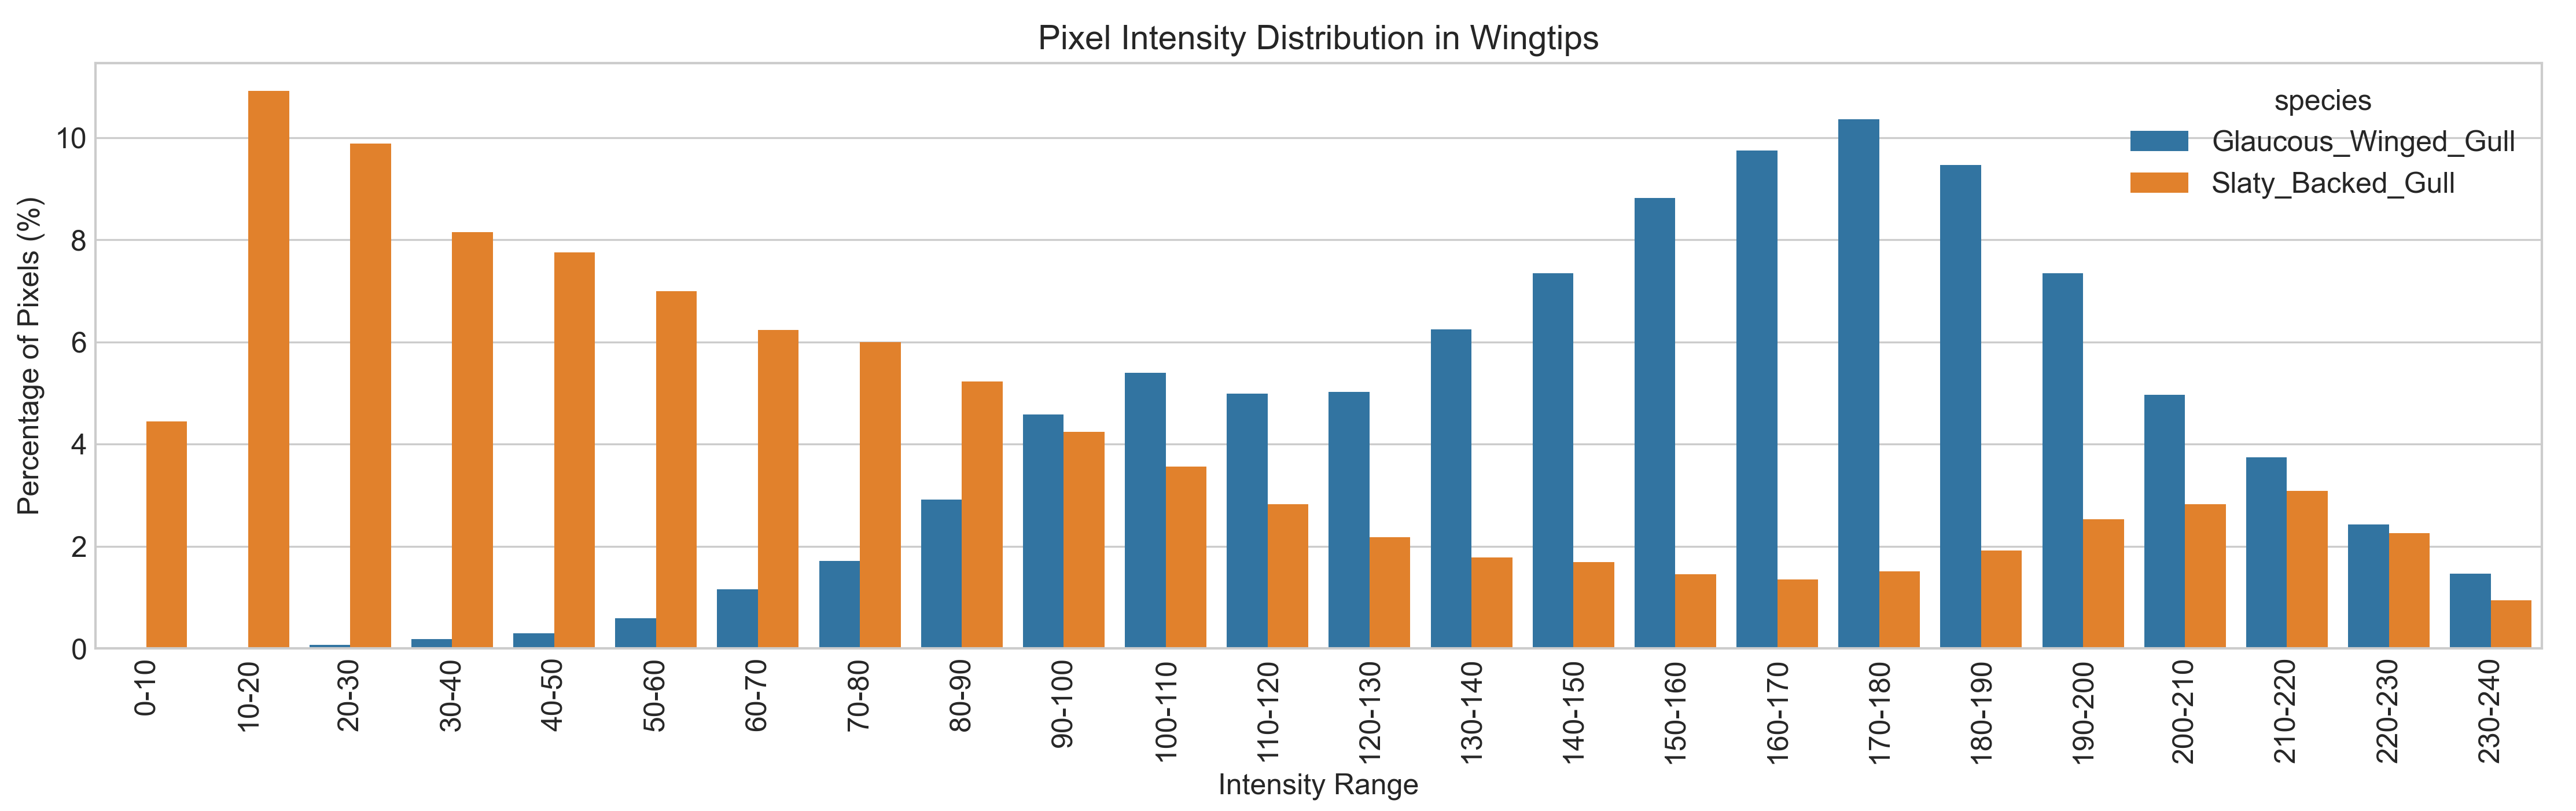
\includegraphics[width=\textwidth]{images/REPORT_IMAGES_INTENSITY/I2/TIPdistribution.png}
        \caption{Fine-grained intensity bins}
        \label{fig:wingtip_intensity_distribution_fine}
    \end{subfigure}
    \caption{Distributions of wingtip pixel intensities for Slaty-backed Gulls (orange) and Glaucous-winged Gulls (blue) using (a) grouped and (b) fine-grained intensity bins.}
    \label{fig:wingtip_intensity_distributions}
\end{figure}

\subsection{Presence of Very Dark Pixels}

A detailed analysis of wingtip pixel intensity reveals a striking difference in the prevalence of very dark pixels between Slaty-backed Gulls and Glaucous-winged Gulls. As shown in Figure~\ref{fig:pixels_below_thresh}, Slaty-backed Gulls have a much higher percentage of wingtip pixels below each intensity threshold examined ($<$30, $<$40, $<$50, $<$60), with values rising from 25\% to nearly 48\%. In contrast, Glaucous-winged Gulls have negligible proportions of such dark pixels at all thresholds.

Figure~\ref{fig:verydarkdist} further demonstrates that this difference is consistent across all sub-ranges within the very dark pixel spectrum (0--60), with Slaty-backed Gulls consistently showing a substantially greater percentage of pixels in each bin.


\begin{figure}[H]
    \centering
    \begin{subfigure}[b]{0.48\textwidth}
        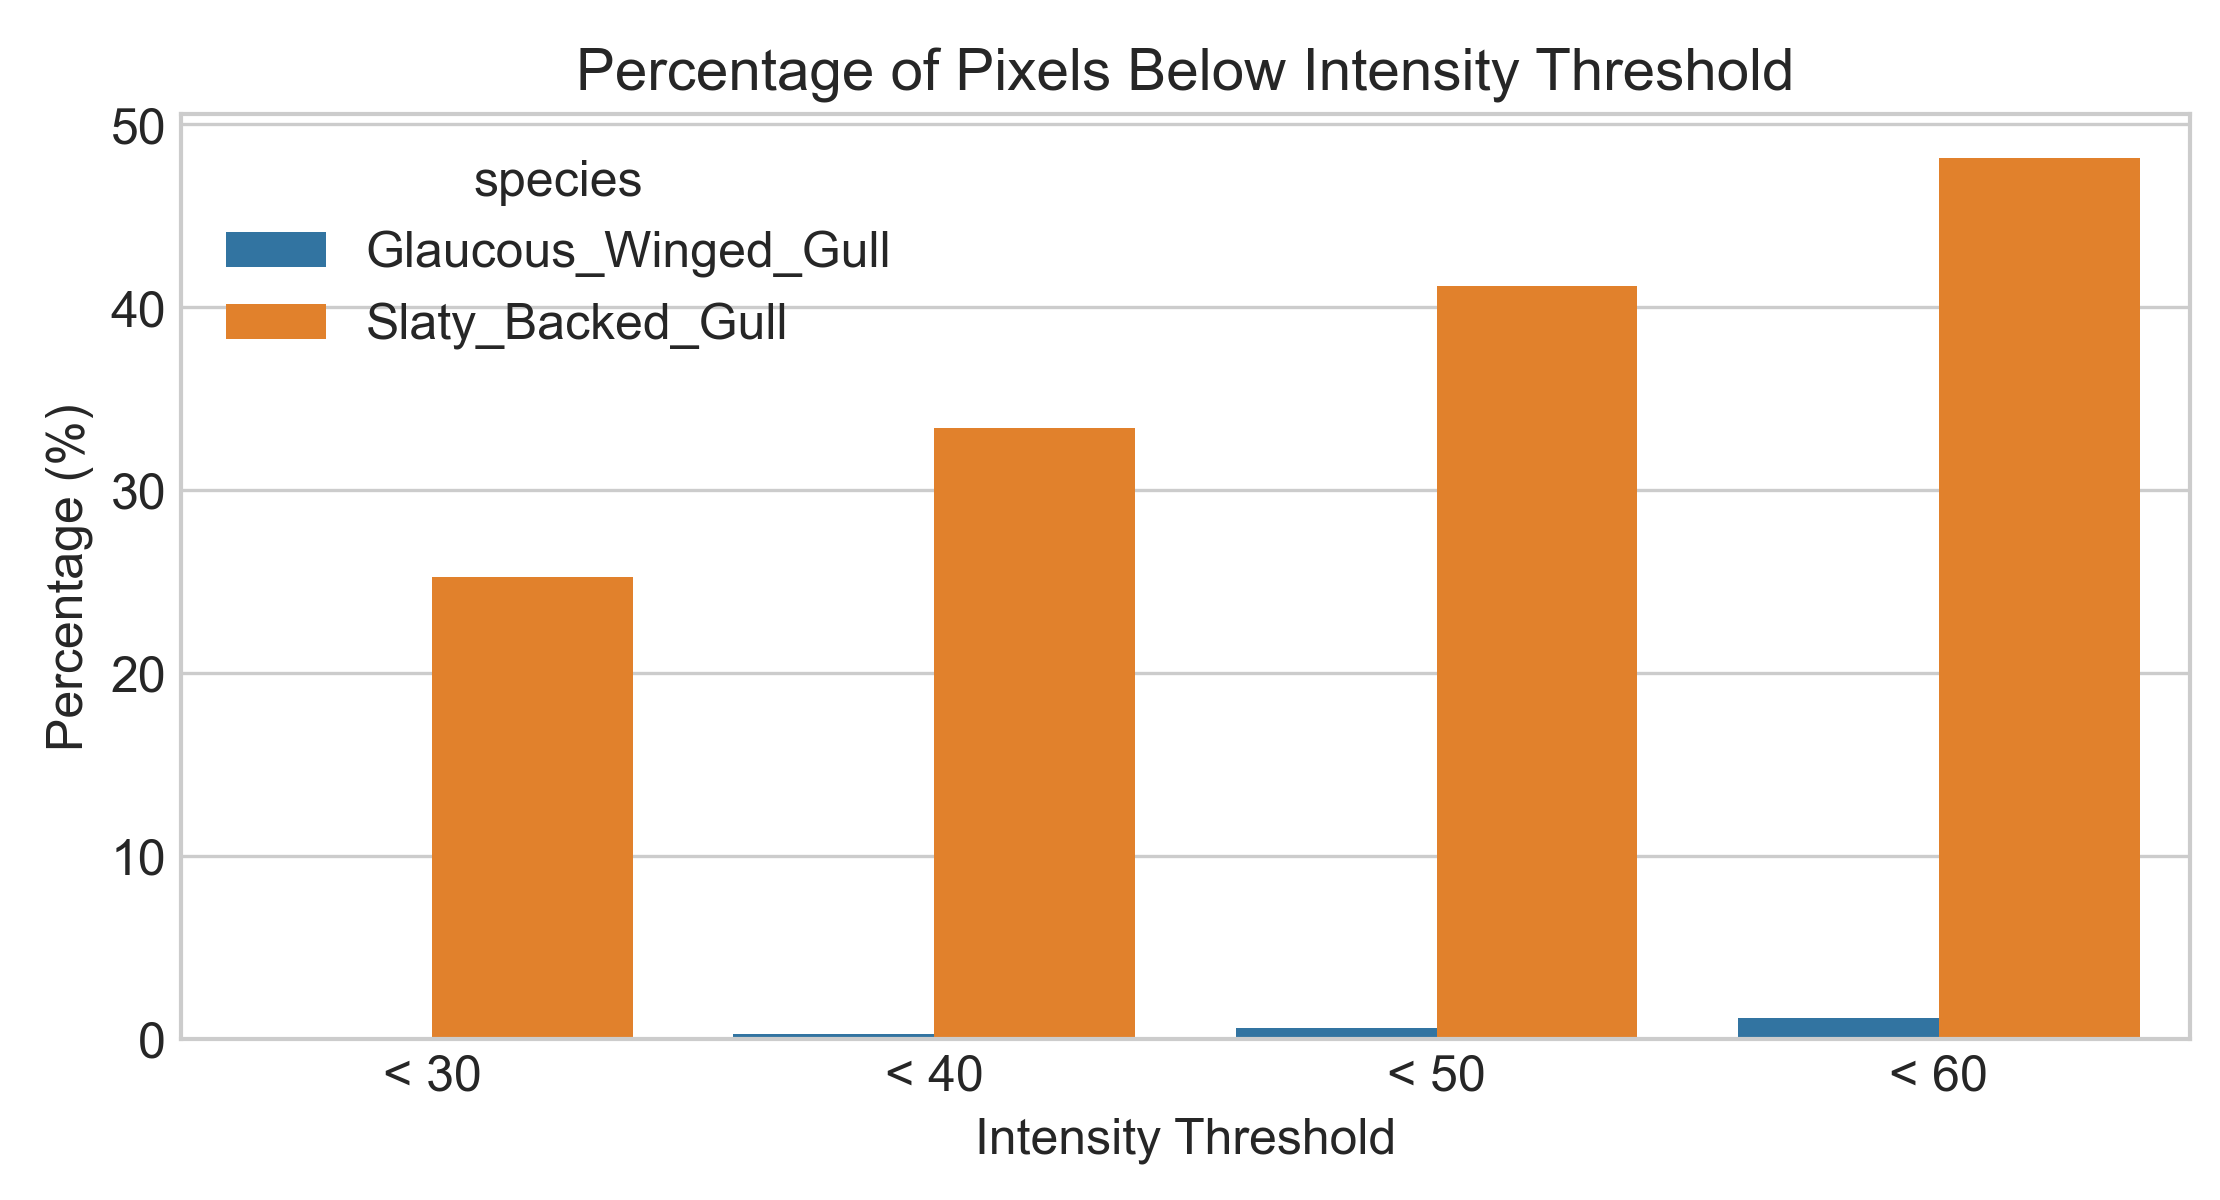
\includegraphics[width=\textwidth]{images/REPORT_IMAGES_INTENSITY/I2/pixelsbelowthresh.png}
        \caption{Percentage of wingtip pixels below each intensity threshold.}
        \label{fig:pixels_below_thresh}
    \end{subfigure}
    \hfill
    \begin{subfigure}[b]{0.48\textwidth}
        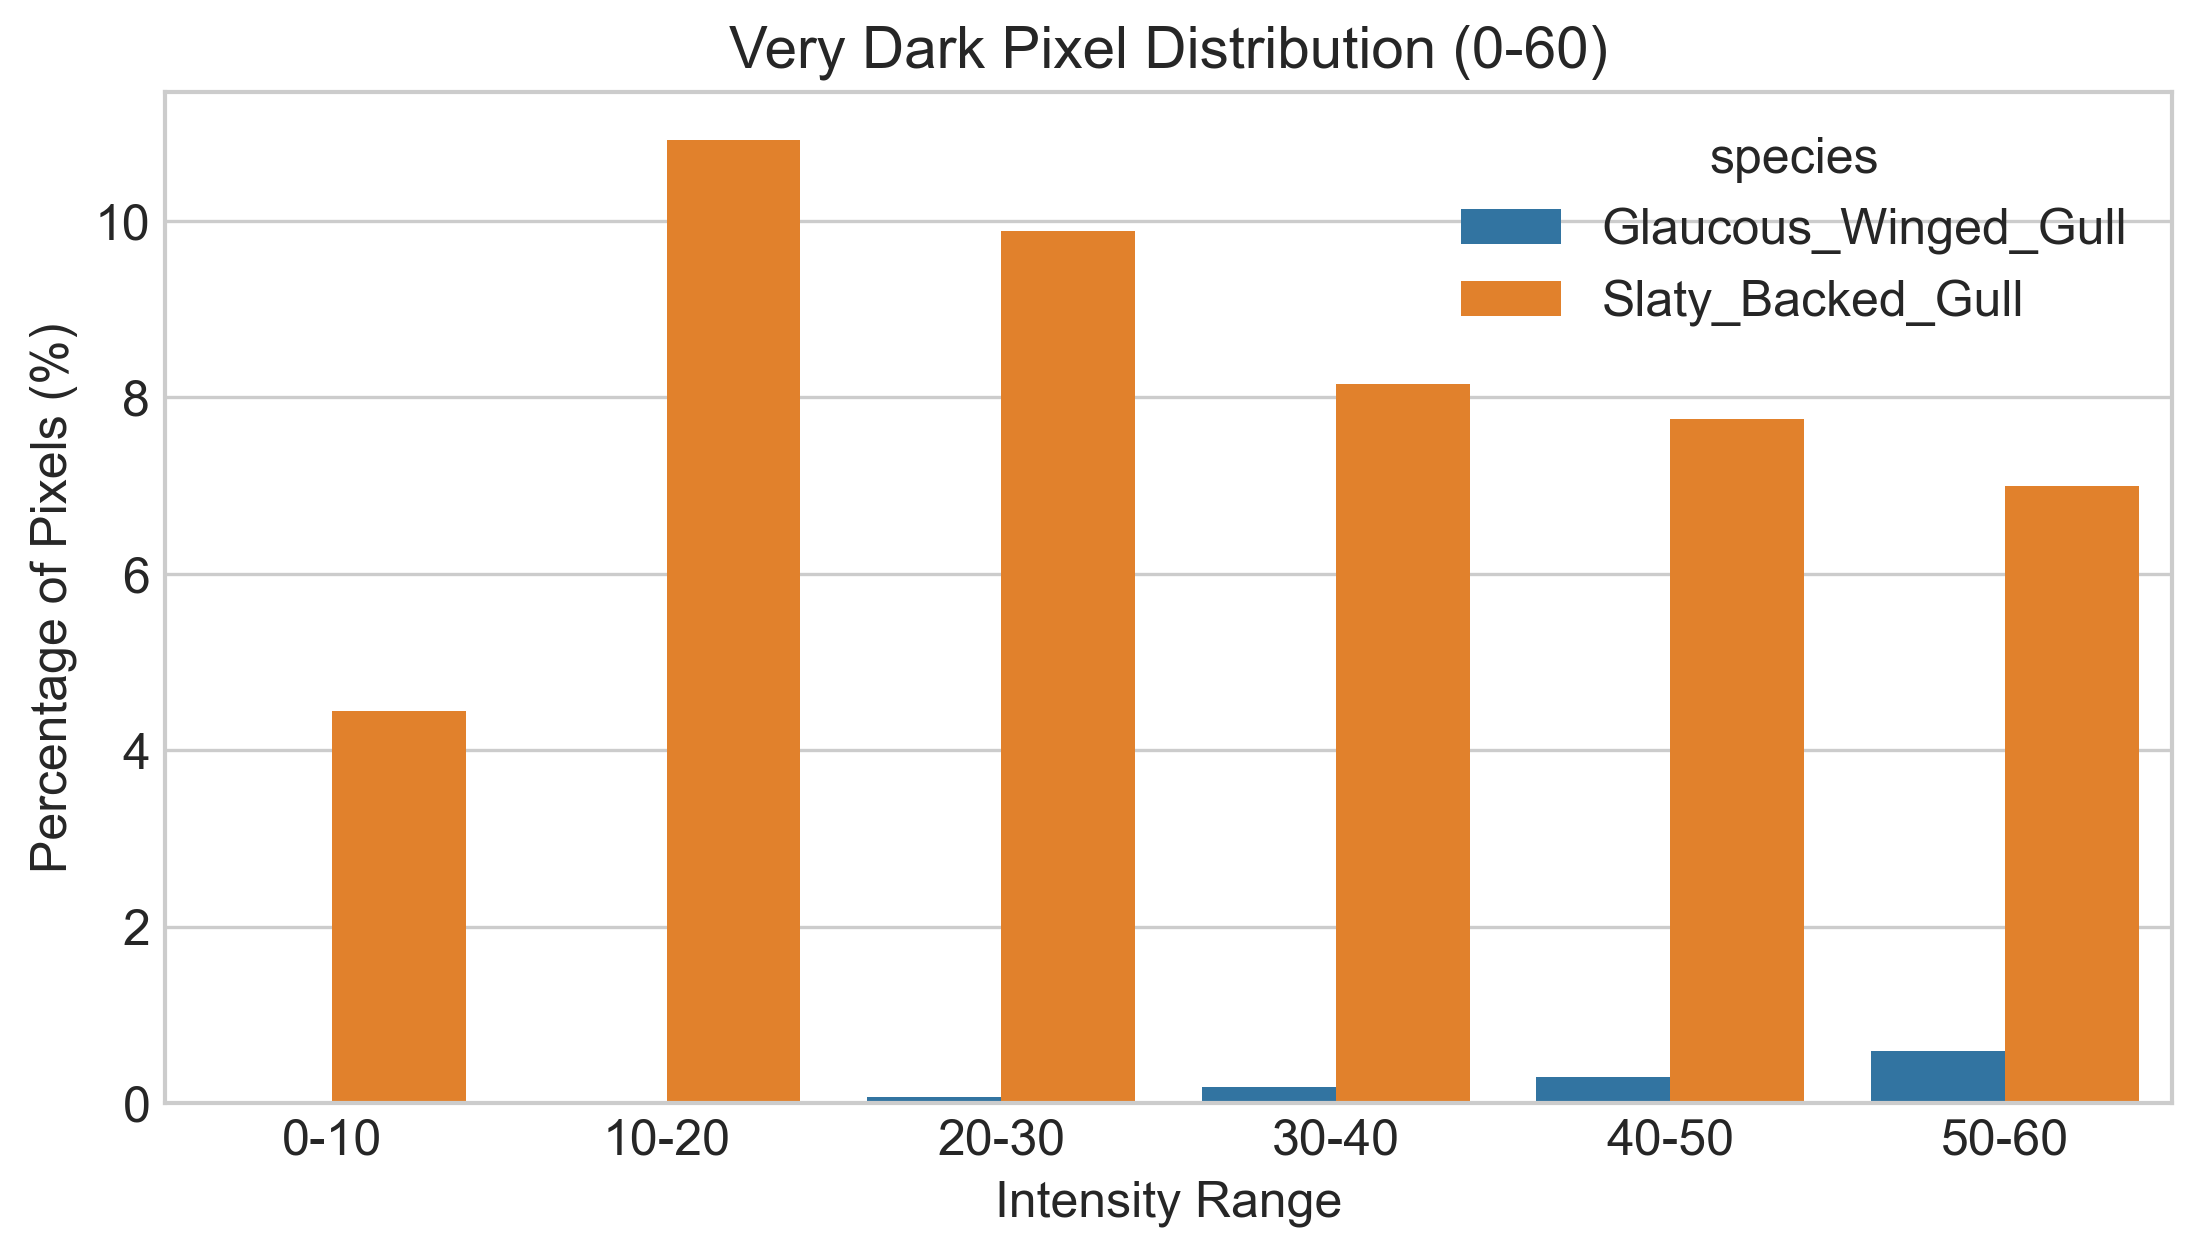
\includegraphics[width=\textwidth]{images/REPORT_IMAGES_INTENSITY/I2/verydarkdist.png}
        \caption{Distribution of very dark pixels (0--60) in wingtip regions.}
        \label{fig:verydarkdist}
    \end{subfigure}
    \caption{Comparison of very dark pixel proportions in wingtip regions for Slaty-backed and Glaucous-winged Gulls.}
\end{figure}

\begin{figure}[H]
    \centering
    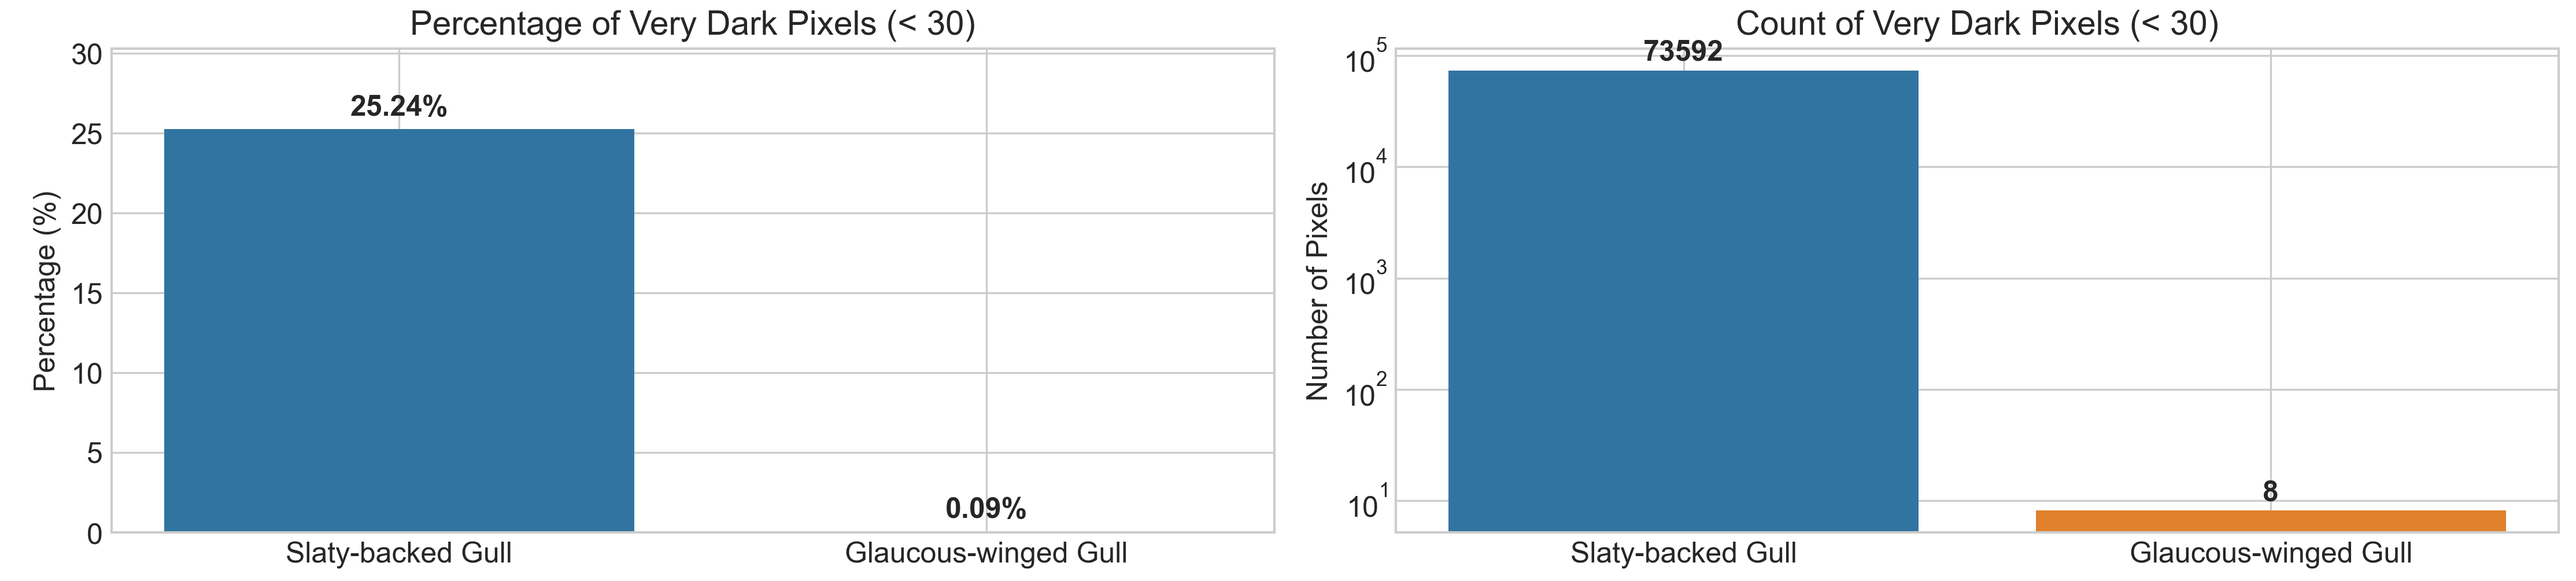
\includegraphics[width=0.9\textwidth]{images/REPORT_IMAGES_INTENSITY/I2/darkpixels.png}
    \caption{Left: Percentage of very dark pixels ($<$30) by species. Right: Average count of very dark pixels ($<$30) per wingtip region, shown on a logarithmic scale.}
    \label{fig:darkpixels}
\end{figure}

The quantitative difference in very dark pixels between species is substantial, as shown in Figure~\ref{fig:darkpixels}, with Slaty-backed Gulls having on average 73,592 very dark pixels compared to just 8 in Glaucous-winged Gulls. This represents a critical diagnostic feature for species identification. This pronounced disparity represents a critical diagnostic feature for species identification. However, it is important to note that the presence of very dark pixels is not consistent across all images, so this feature may not be used as a distinguishing criterion in every case.

\subsection{Relationship Between Wing and Wingtip Intensities}

To quantitatively assess the relative darkness of wingtip area compared to the rest of the wing which were the 2 critical areas highlighted by Grad-CAM, the proportion of wingtip pixels that are darker than the mean wing intensity for each species was calculated as suggested by industry expert Professor Gibbins.  The results are presented in Table~\ref{tab:darknessproportion}. 


\begin{table}[H]
    \centering
    \caption{Proportion of Wingtip Pixels Darker than Mean Wing Intensity}
    \label{tab:darknessproportion}
    \begin{tabular}{lcc}
        \toprule
        Species & Percentage \\
        \midrule
        Slaty-backed Gull & 56.69\% \\
        Glaucous-winged Gull & 47.71\% \\
        \bottomrule
    \end{tabular}
\end{table}

Figure~\ref{fig:wing_vs_wingtip_intensity} visualizes the relationship between mean wing intensity and mean wingtip intensity for individual birds. The dashed line indicates equal intensity between wing and wingtip. As illustrated, there is a strong positive correlation between wing and wingtip intensities across both species; as the mean wing intensity increases, the mean wingtip intensity also increases. This pattern suggests that, in most cases, the relative difference in darkness between the wing and wingtip results only in a slight difference in the proportion of darker wingtip pixels between the two species.

\begin{figure}[H]
    \centering
    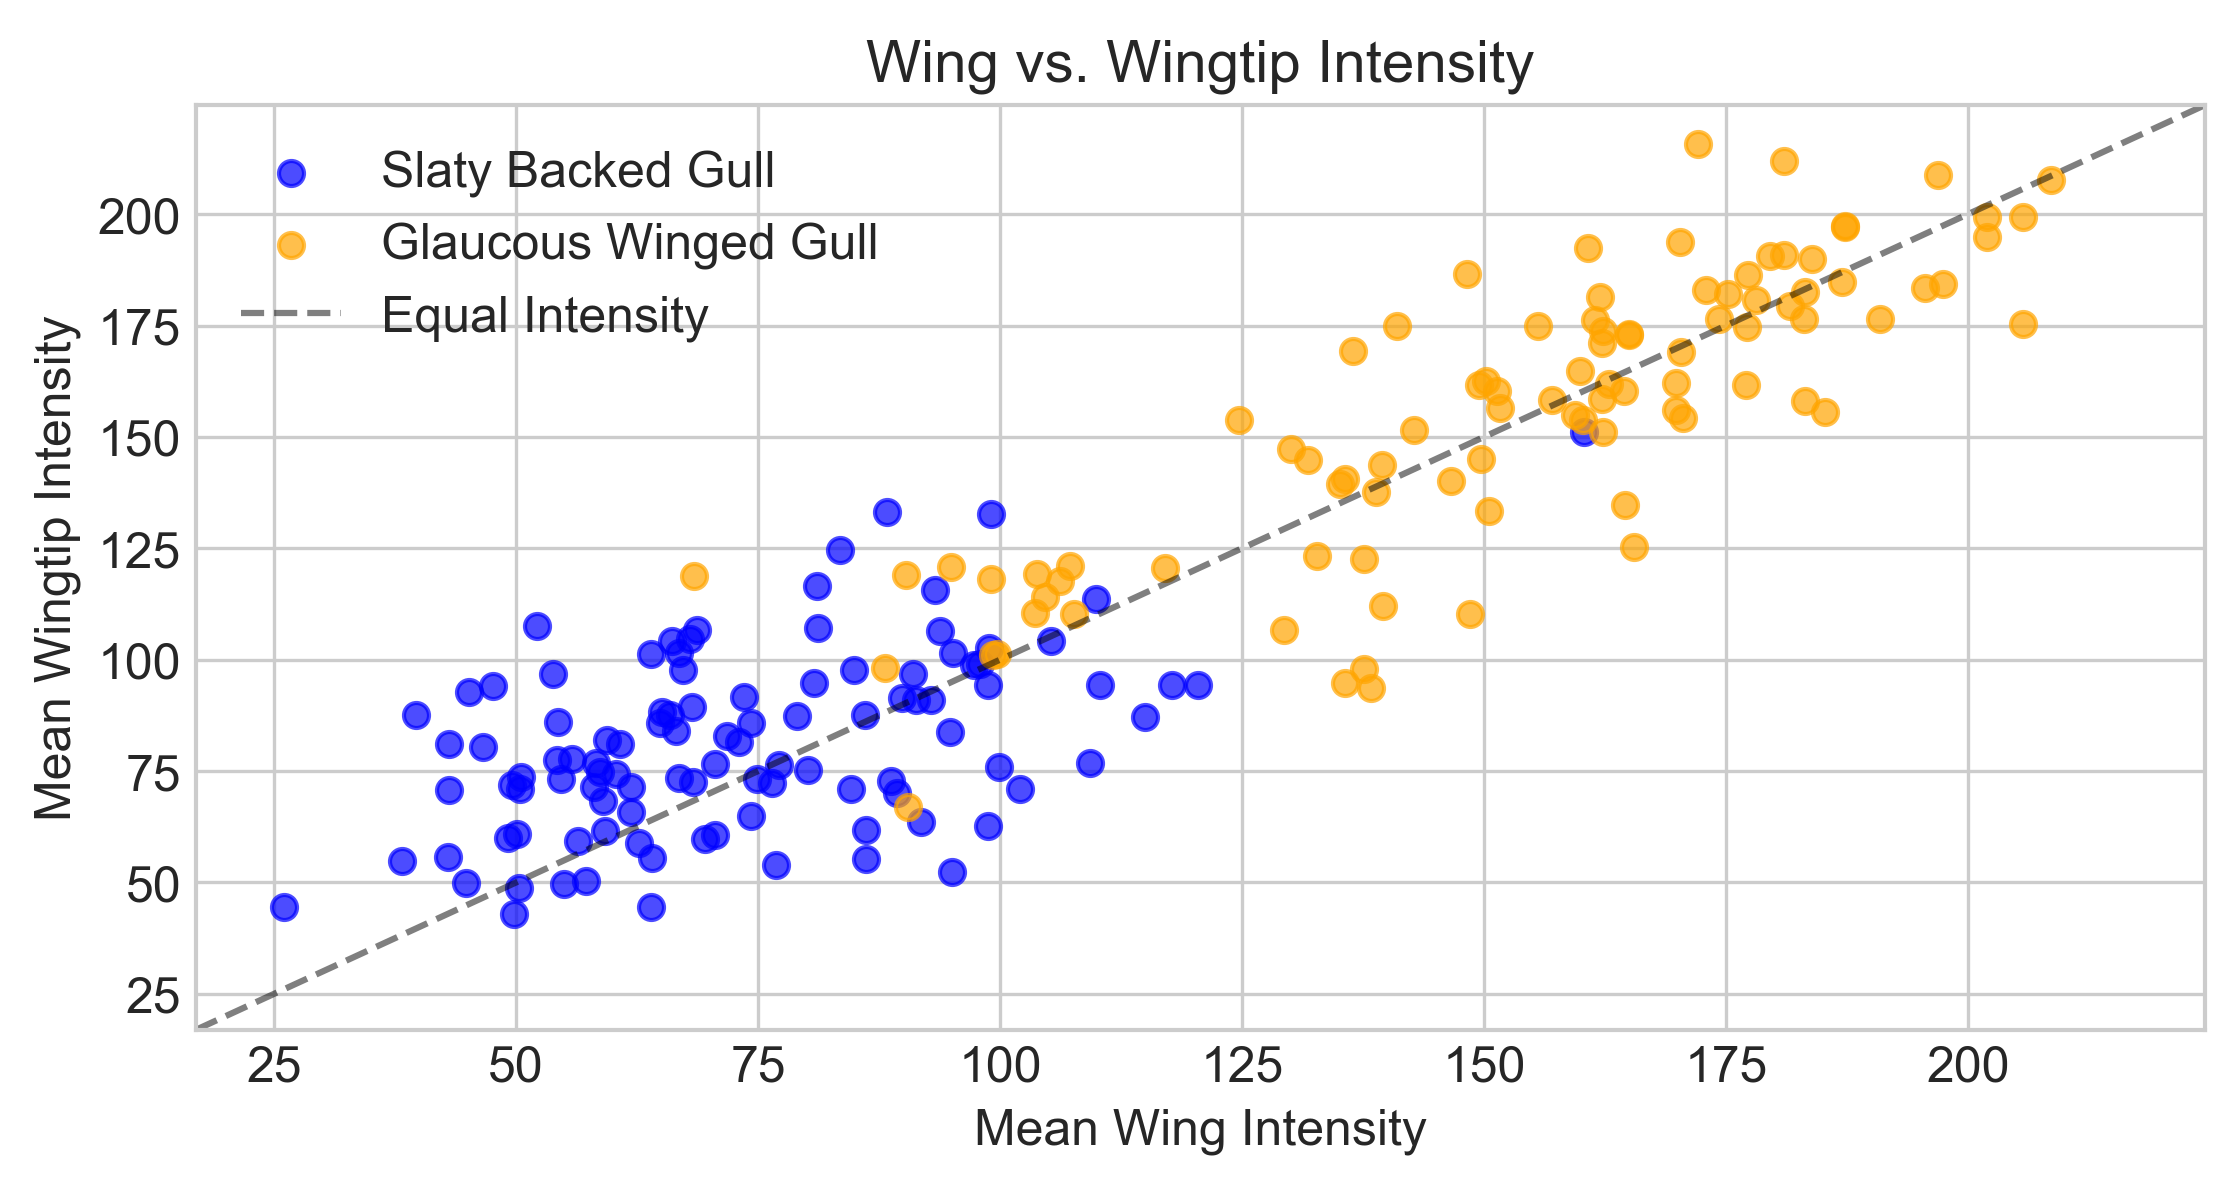
\includegraphics[width=0.55\textwidth]{images/REPORT_IMAGES_INTENSITY/I2/clusterwingwingtip.png}
    \caption{Scatter plot of mean wing intensity vs. mean wingtip intensity for Slaty-backed Gulls (blue) and Glaucous-winged Gulls (orange). The dashed line indicates equal intensity between wing and wingtip.}
    \label{fig:wing_vs_wingtip_intensity}
\end{figure}

\subsection{Wingtip Contrast and Darkness Feature Comparison}

To comprehensively compare the wingtip characteristics distinguishing Slaty-backed and Glaucous-winged Gulls, we analyzed two key features: (1) the proportion of wingtip pixels that are darker than the wing by varying intensity thresholds, and (2) the proportion of pixels that are absolutely dark, below fixed intensity values.

Figure~\ref{fig:wingtip_darkness_summary} presents a set of visualizations summarizing these metrics for both species. The heatmap in subfigure~\ref{fig:intensity_heatmap} displays, on the left, the percentage of wingtip pixels darker than the wing by various thresholds, and on the right, the percentage of absolutely dark pixels. Subfigure~\ref{fig:diff_bar} shows the absolute difference in the proportion of dark pixels between species at each threshold, while subfigure~\ref{fig:diff_curve} plots the difference curve (Slaty-backed minus Glaucous-winged) across thresholds, highlighting where the species gap is largest. Subfigure~\ref{fig:ratio_plot} quantifies the relative difference by showing the ratio of dark pixel proportions (Slaty-backed/Glaucous-winged) at each threshold, with the ratio peaking near 2.8--2.9$\times$ between thresholds of 50 and 80. Collectively, these visualizations demonstrate that Slaty-backed Gulls consistently have a much higher proportion of both strongly contrasting and absolutely dark pixels, making these features highly discriminative.

\begin{figure}[H]
    \centering
    % (a) Heatmap
    \begin{subfigure}[b]{0.48\textwidth}
        \centering
        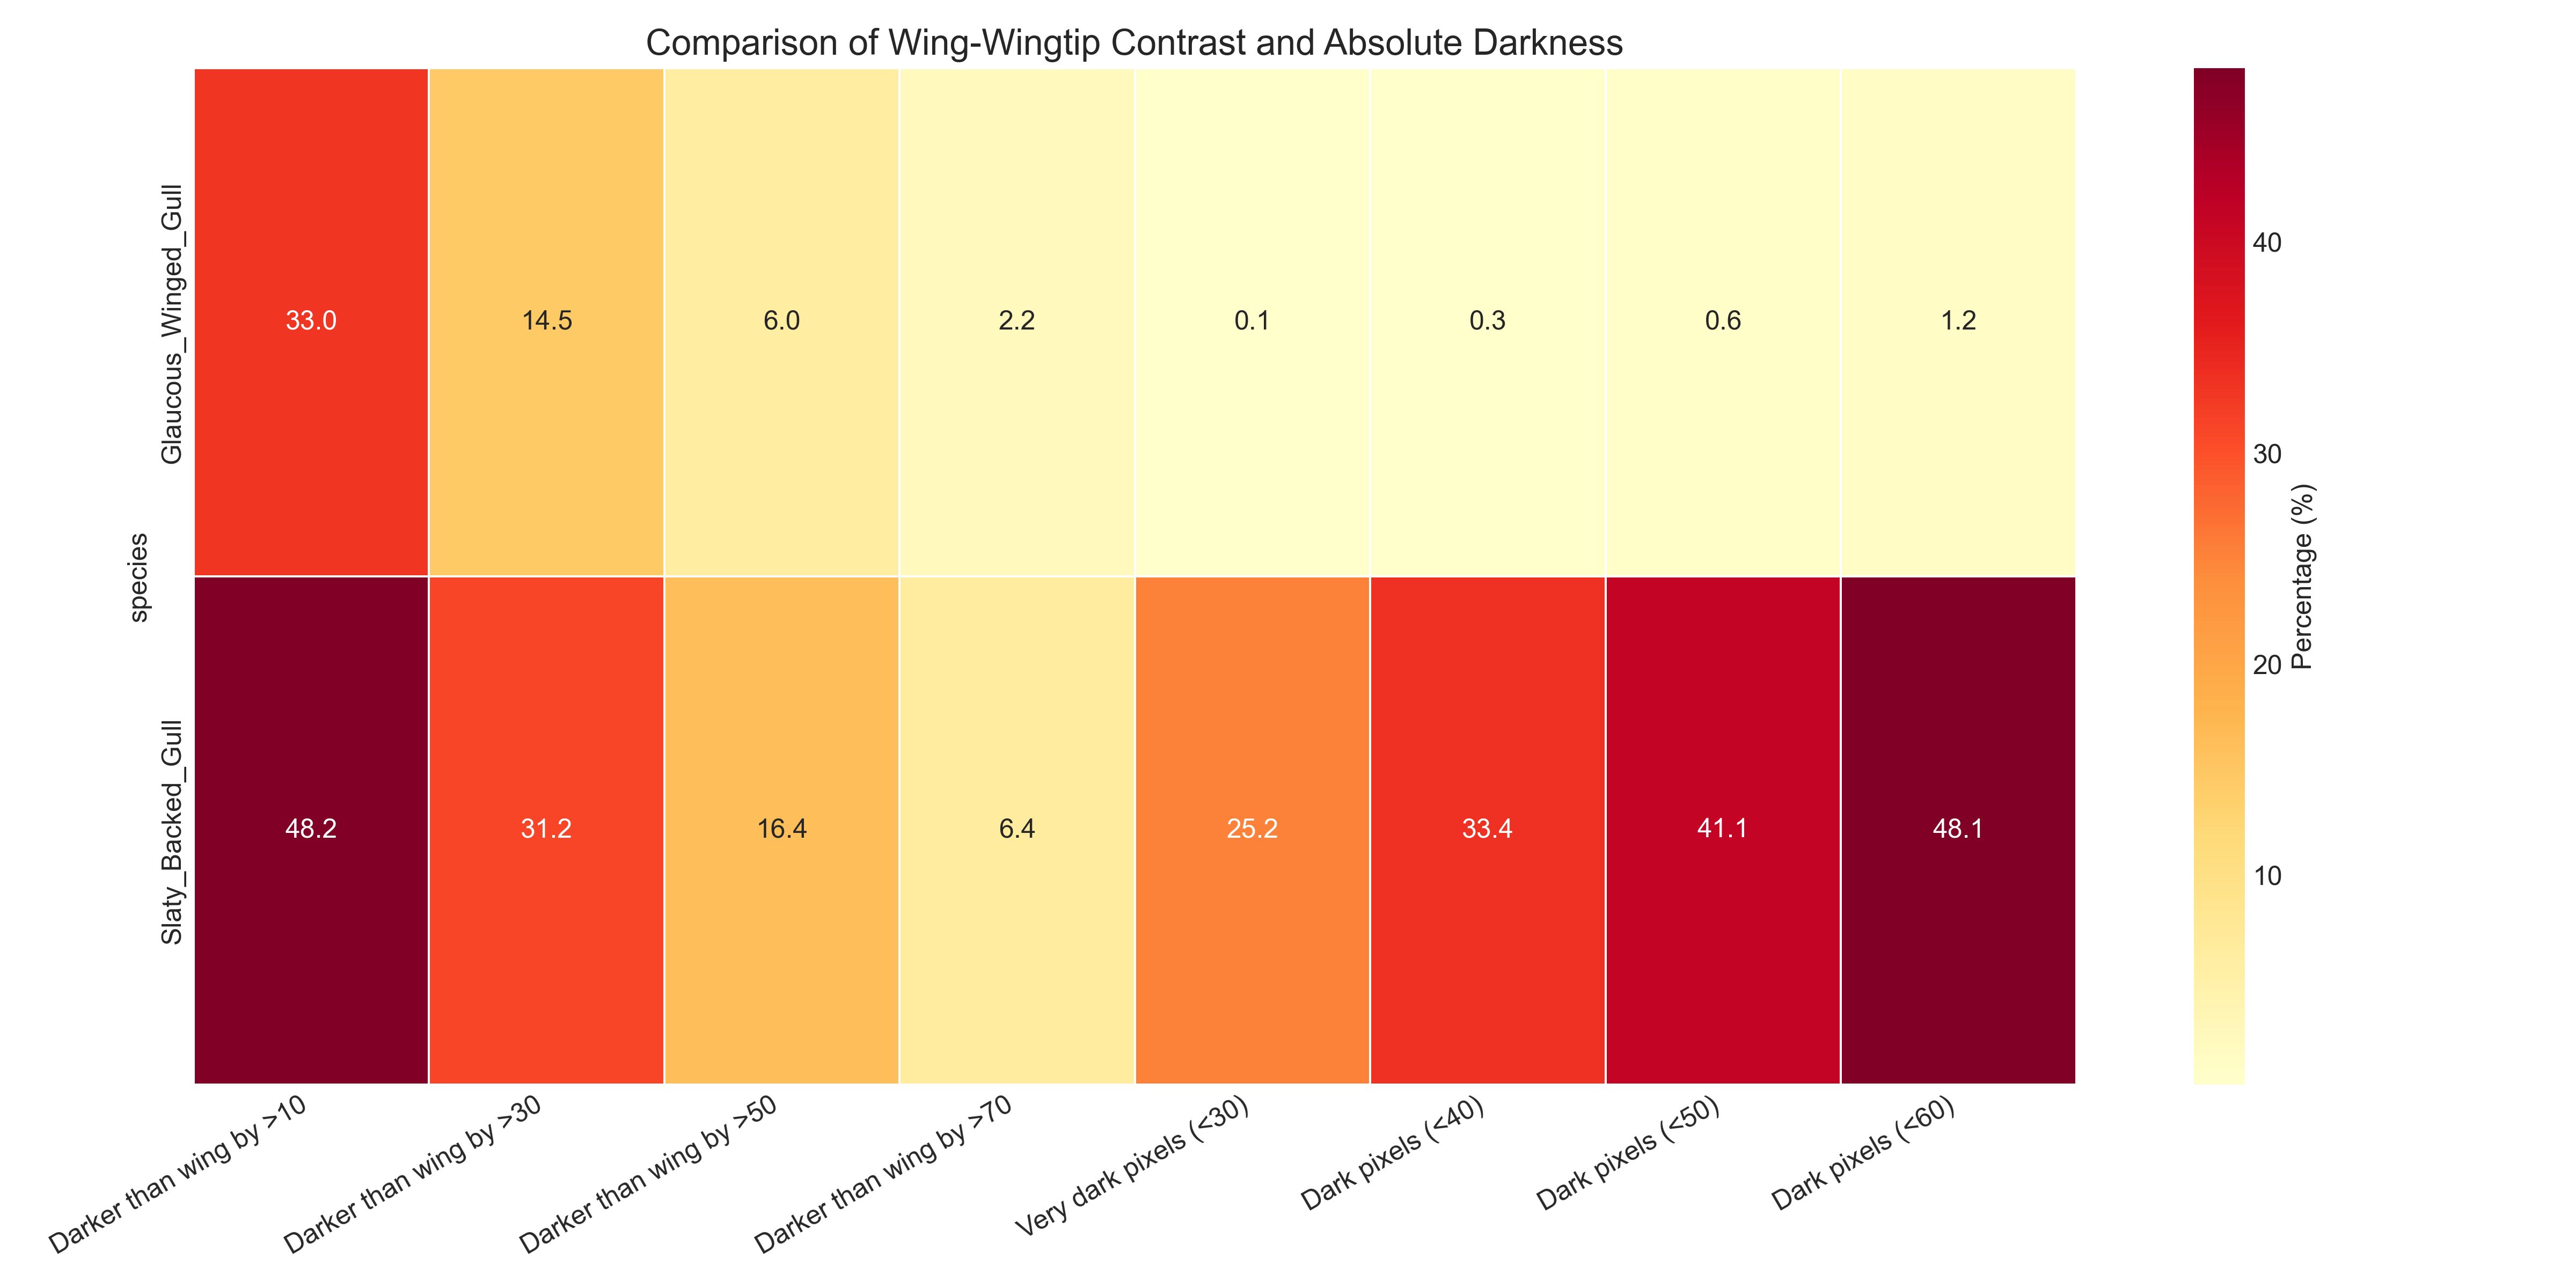
\includegraphics[width=\textwidth]{images/REPORT_IMAGES_INTENSITY/I1/wingtip_darkness_heatmap.png}
        \caption{Heatmap of wingtip darkness and contrast features for each species.}
        \label{fig:intensity_heatmap}
    \end{subfigure}
    \hfill
    % (b) Difference bar plot
    \begin{subfigure}[b]{0.48\textwidth}
        \centering
        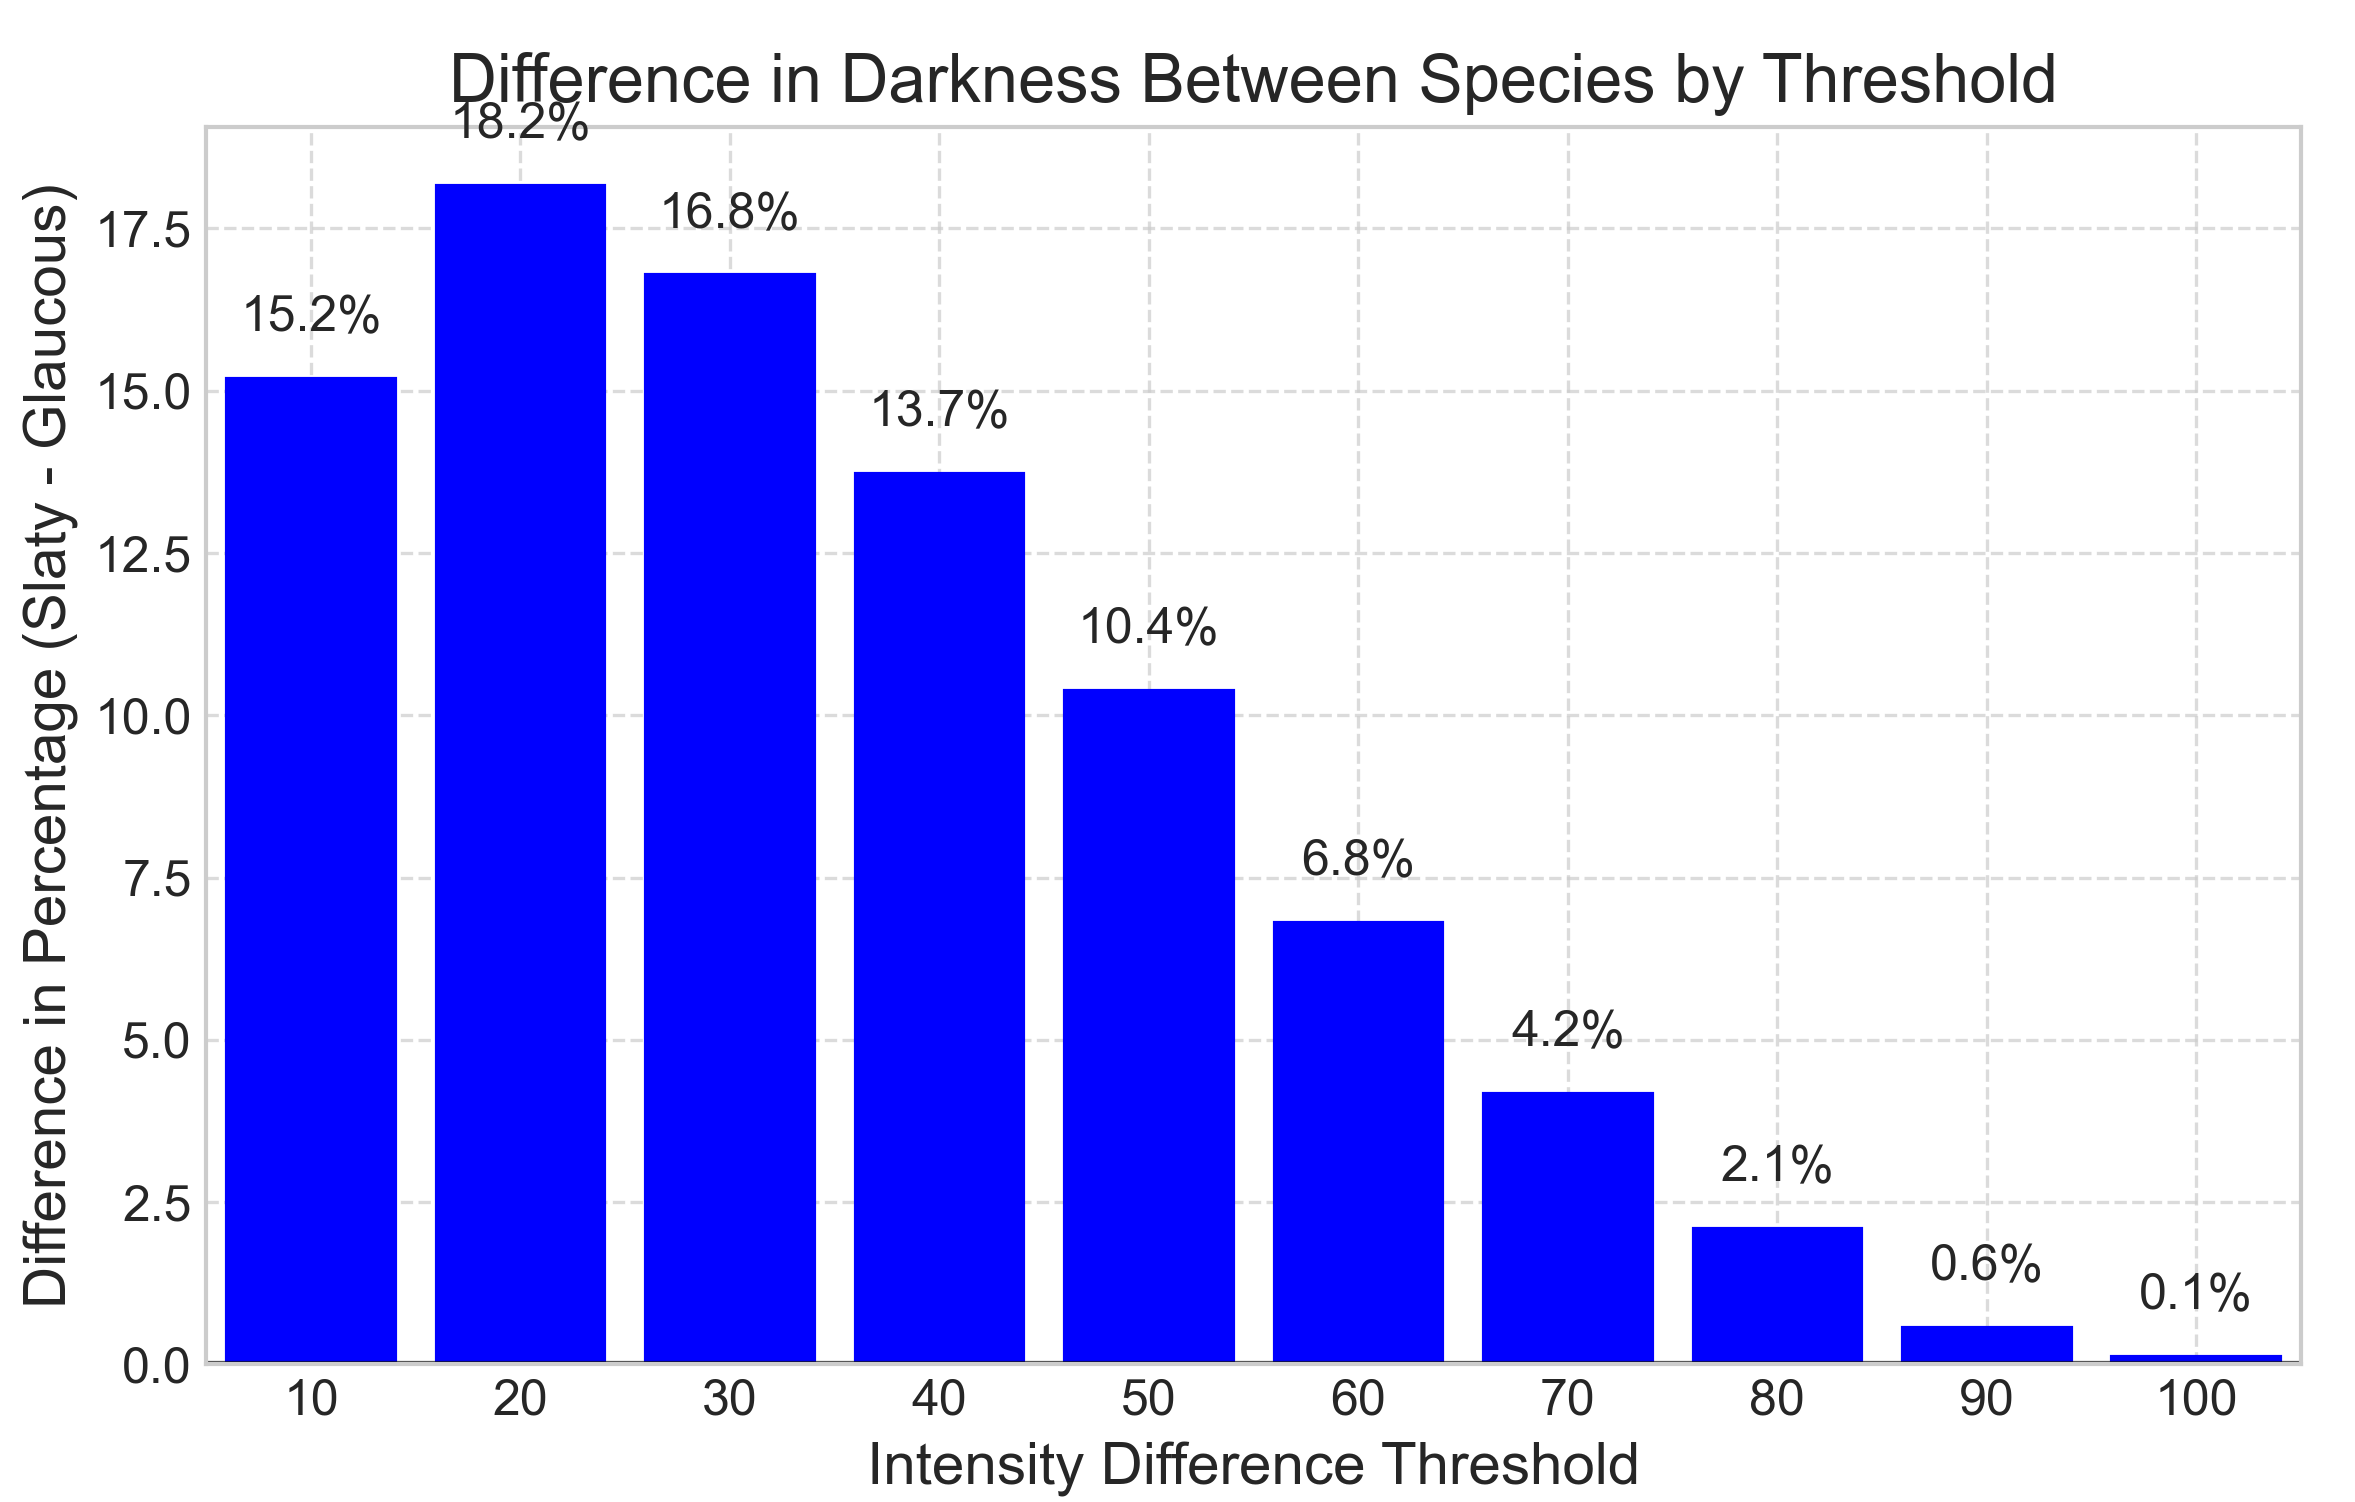
\includegraphics[width=\textwidth]{images/REPORT_IMAGES_INTENSITY/I1/diffbythresh.png}
        \caption{Absolute difference in percentage of dark pixels by threshold.}
        \label{fig:diff_bar}
    \end{subfigure}
    \vspace{1em}
    % (c) Difference curve
    \begin{subfigure}[b]{0.48\textwidth}
        \centering
        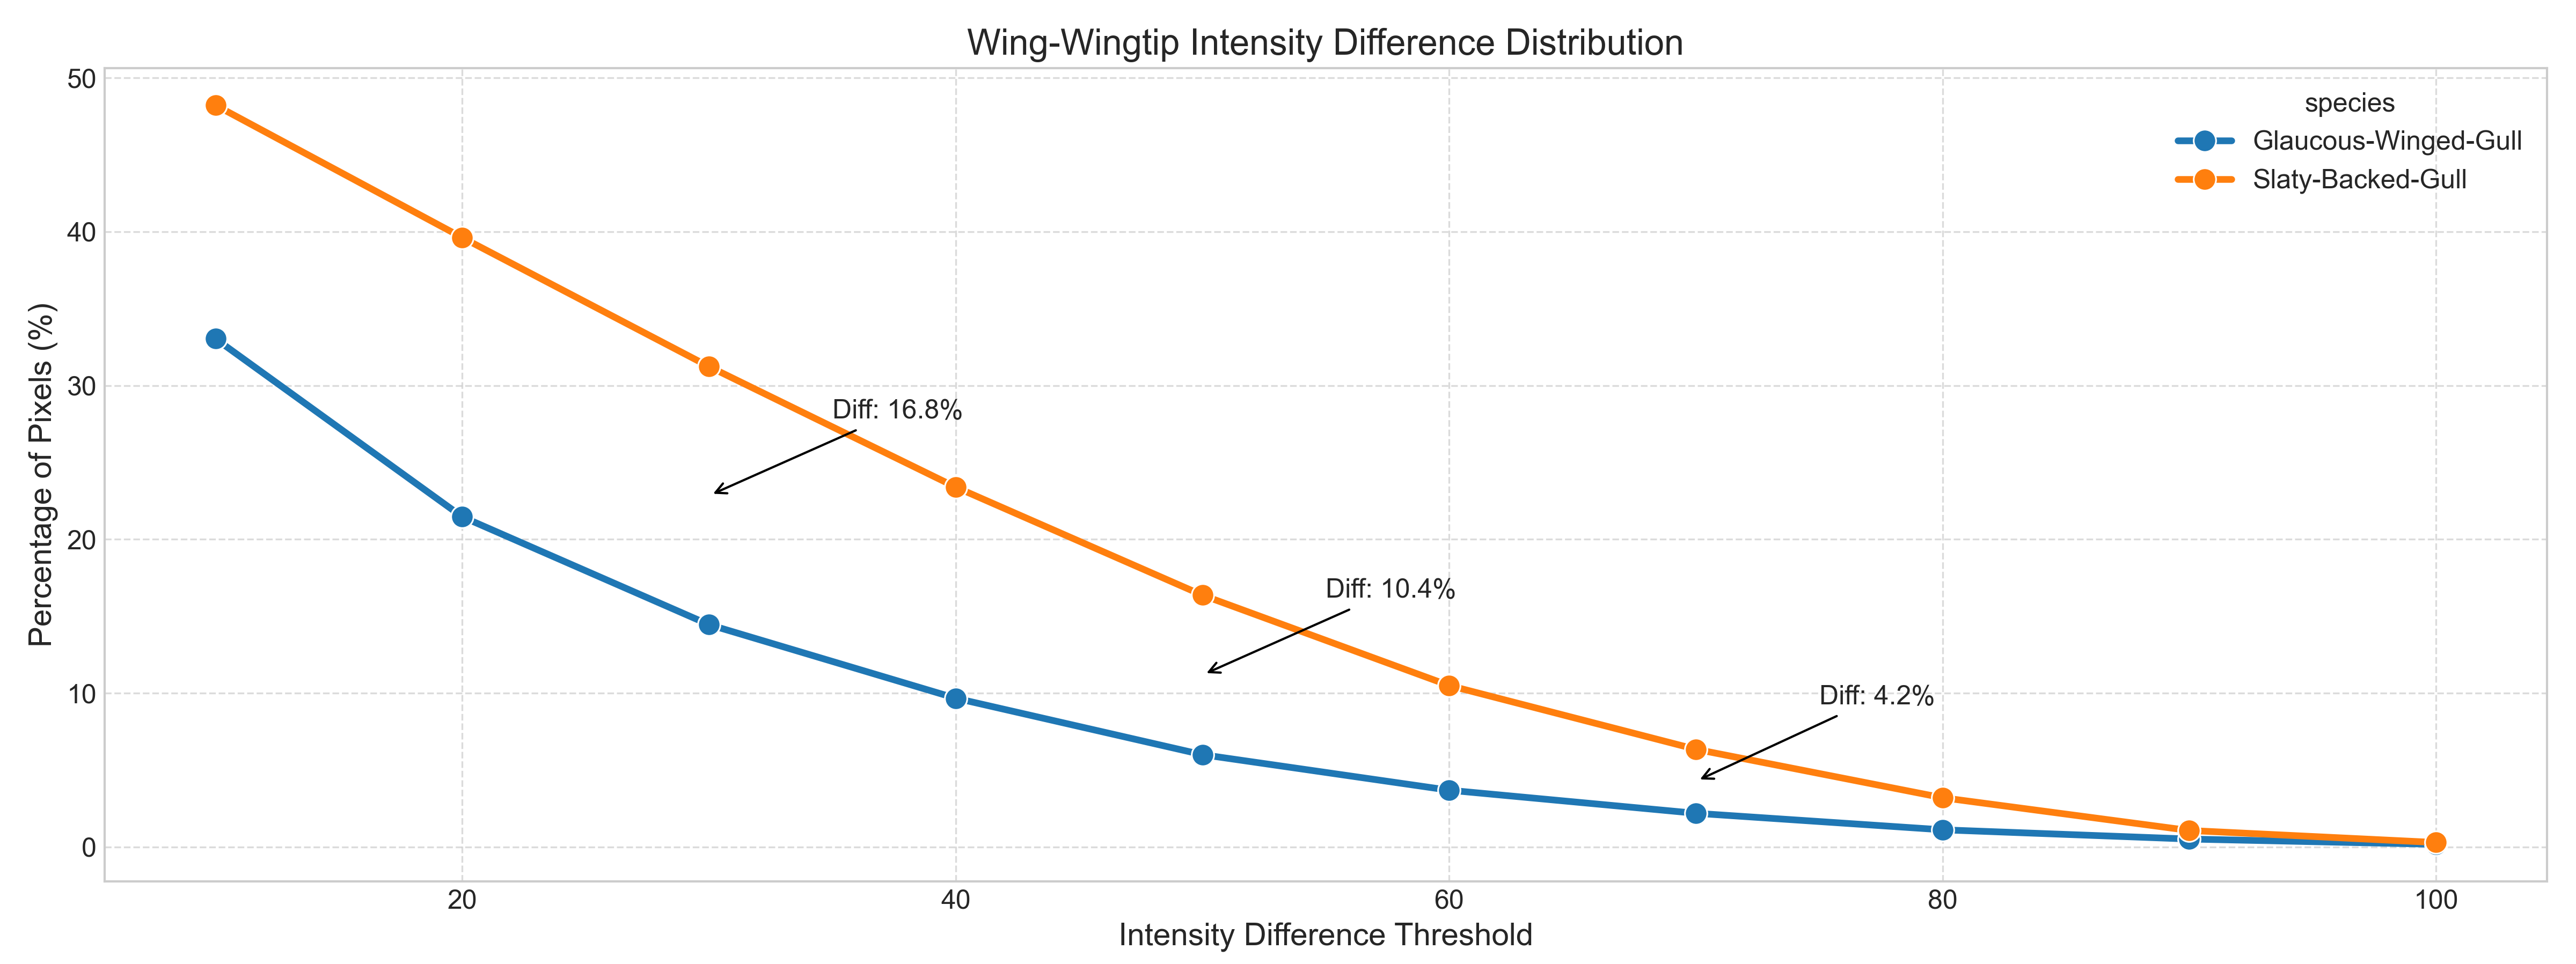
\includegraphics[width=\textwidth]{images/REPORT_IMAGES_INTENSITY/I1/intensitydiffthreshold.png}
        \caption{Difference curve (Slaty-backed minus Glaucous-winged) across thresholds.}
        \label{fig:diff_curve}
    \end{subfigure}
    \hfill
    % (d) Ratio plot
    \begin{subfigure}[b]{0.48\textwidth}
        \centering
        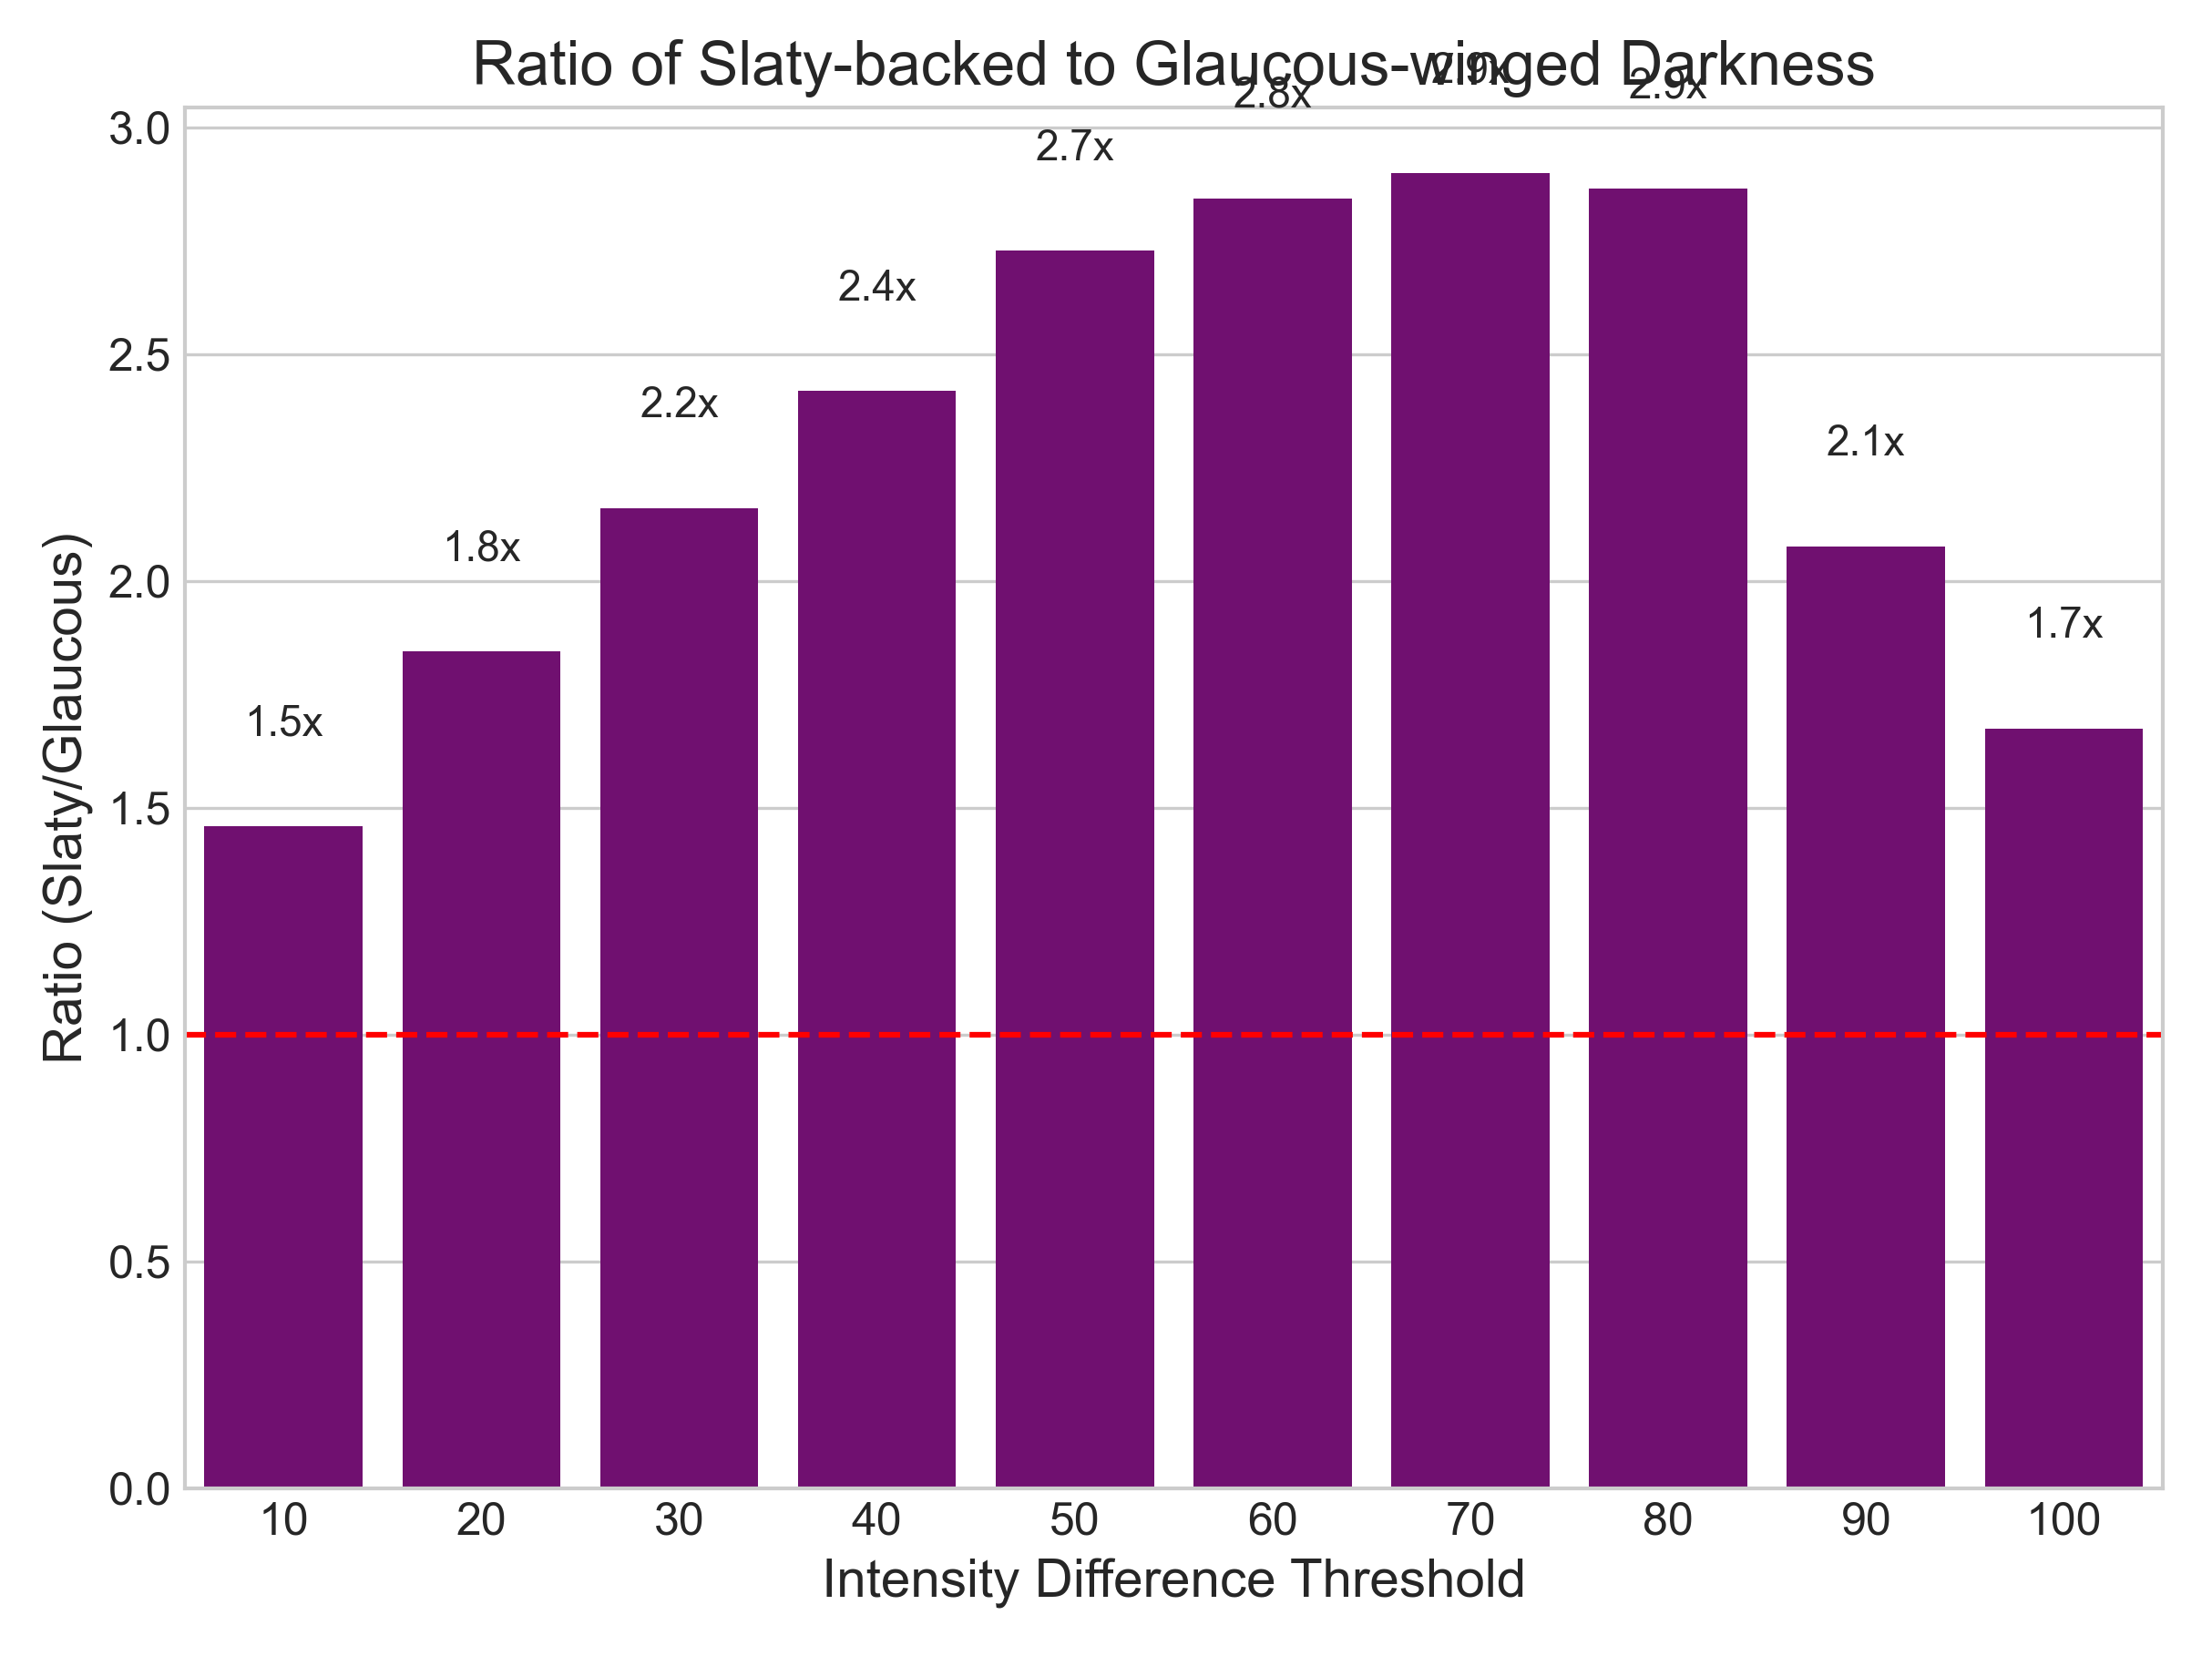
\includegraphics[width=\textwidth]{images/REPORT_IMAGES_INTENSITY/I1/ratiogwgsbgdarkness.png}
        \caption{Ratio of dark pixel proportions (Slaty-backed/Glaucous-winged) by threshold.}
        \label{fig:ratio_plot}
    \end{subfigure}
    \caption{Summary of wingtip darkness and contrast metrics distinguishing Slaty-backed and Glaucous-winged Gulls. (a) Heatmap of key features; (b) absolute difference by threshold; (c) difference curve; (d) ratio of proportions. These visualizations collectively highlight the strong and persistent contrast in wingtip darkness between the two species.}
    \label{fig:wingtip_darkness_summary}
\end{figure}

\section{Results: Local Binary Pattern Texture Analysis}
\label{sec:lbp_results}

% Our Local Binary Pattern (LBP) analysis revealed a few texture differences between Slaty-backed and Glaucous-winged Gulls across anatomical regions. The implementation focused on both ones and transition histograms, with histogram-based feature extraction.

For the final results displayed below, the default LBP variant was selected since default histogram retains all LBP codes, providing a comprehensive representation of local texture patterns. Consequently, it facilitates the direct calculation of derived features such as the number of ones and the number of transitions per pattern, as these statistics can be computed from the complete set of binary codes present in the default histogram. This approach ensures that no potentially discriminative texture information is excluded, thereby supporting a more detailed and flexible analysis of texture complexity and structure across the studied regions.

\subsection{Discriminative Power Analysis}
\begin{figure}[H]
    \centering
    \begin{subfigure}[b]{0.48\textwidth}
        \centering
        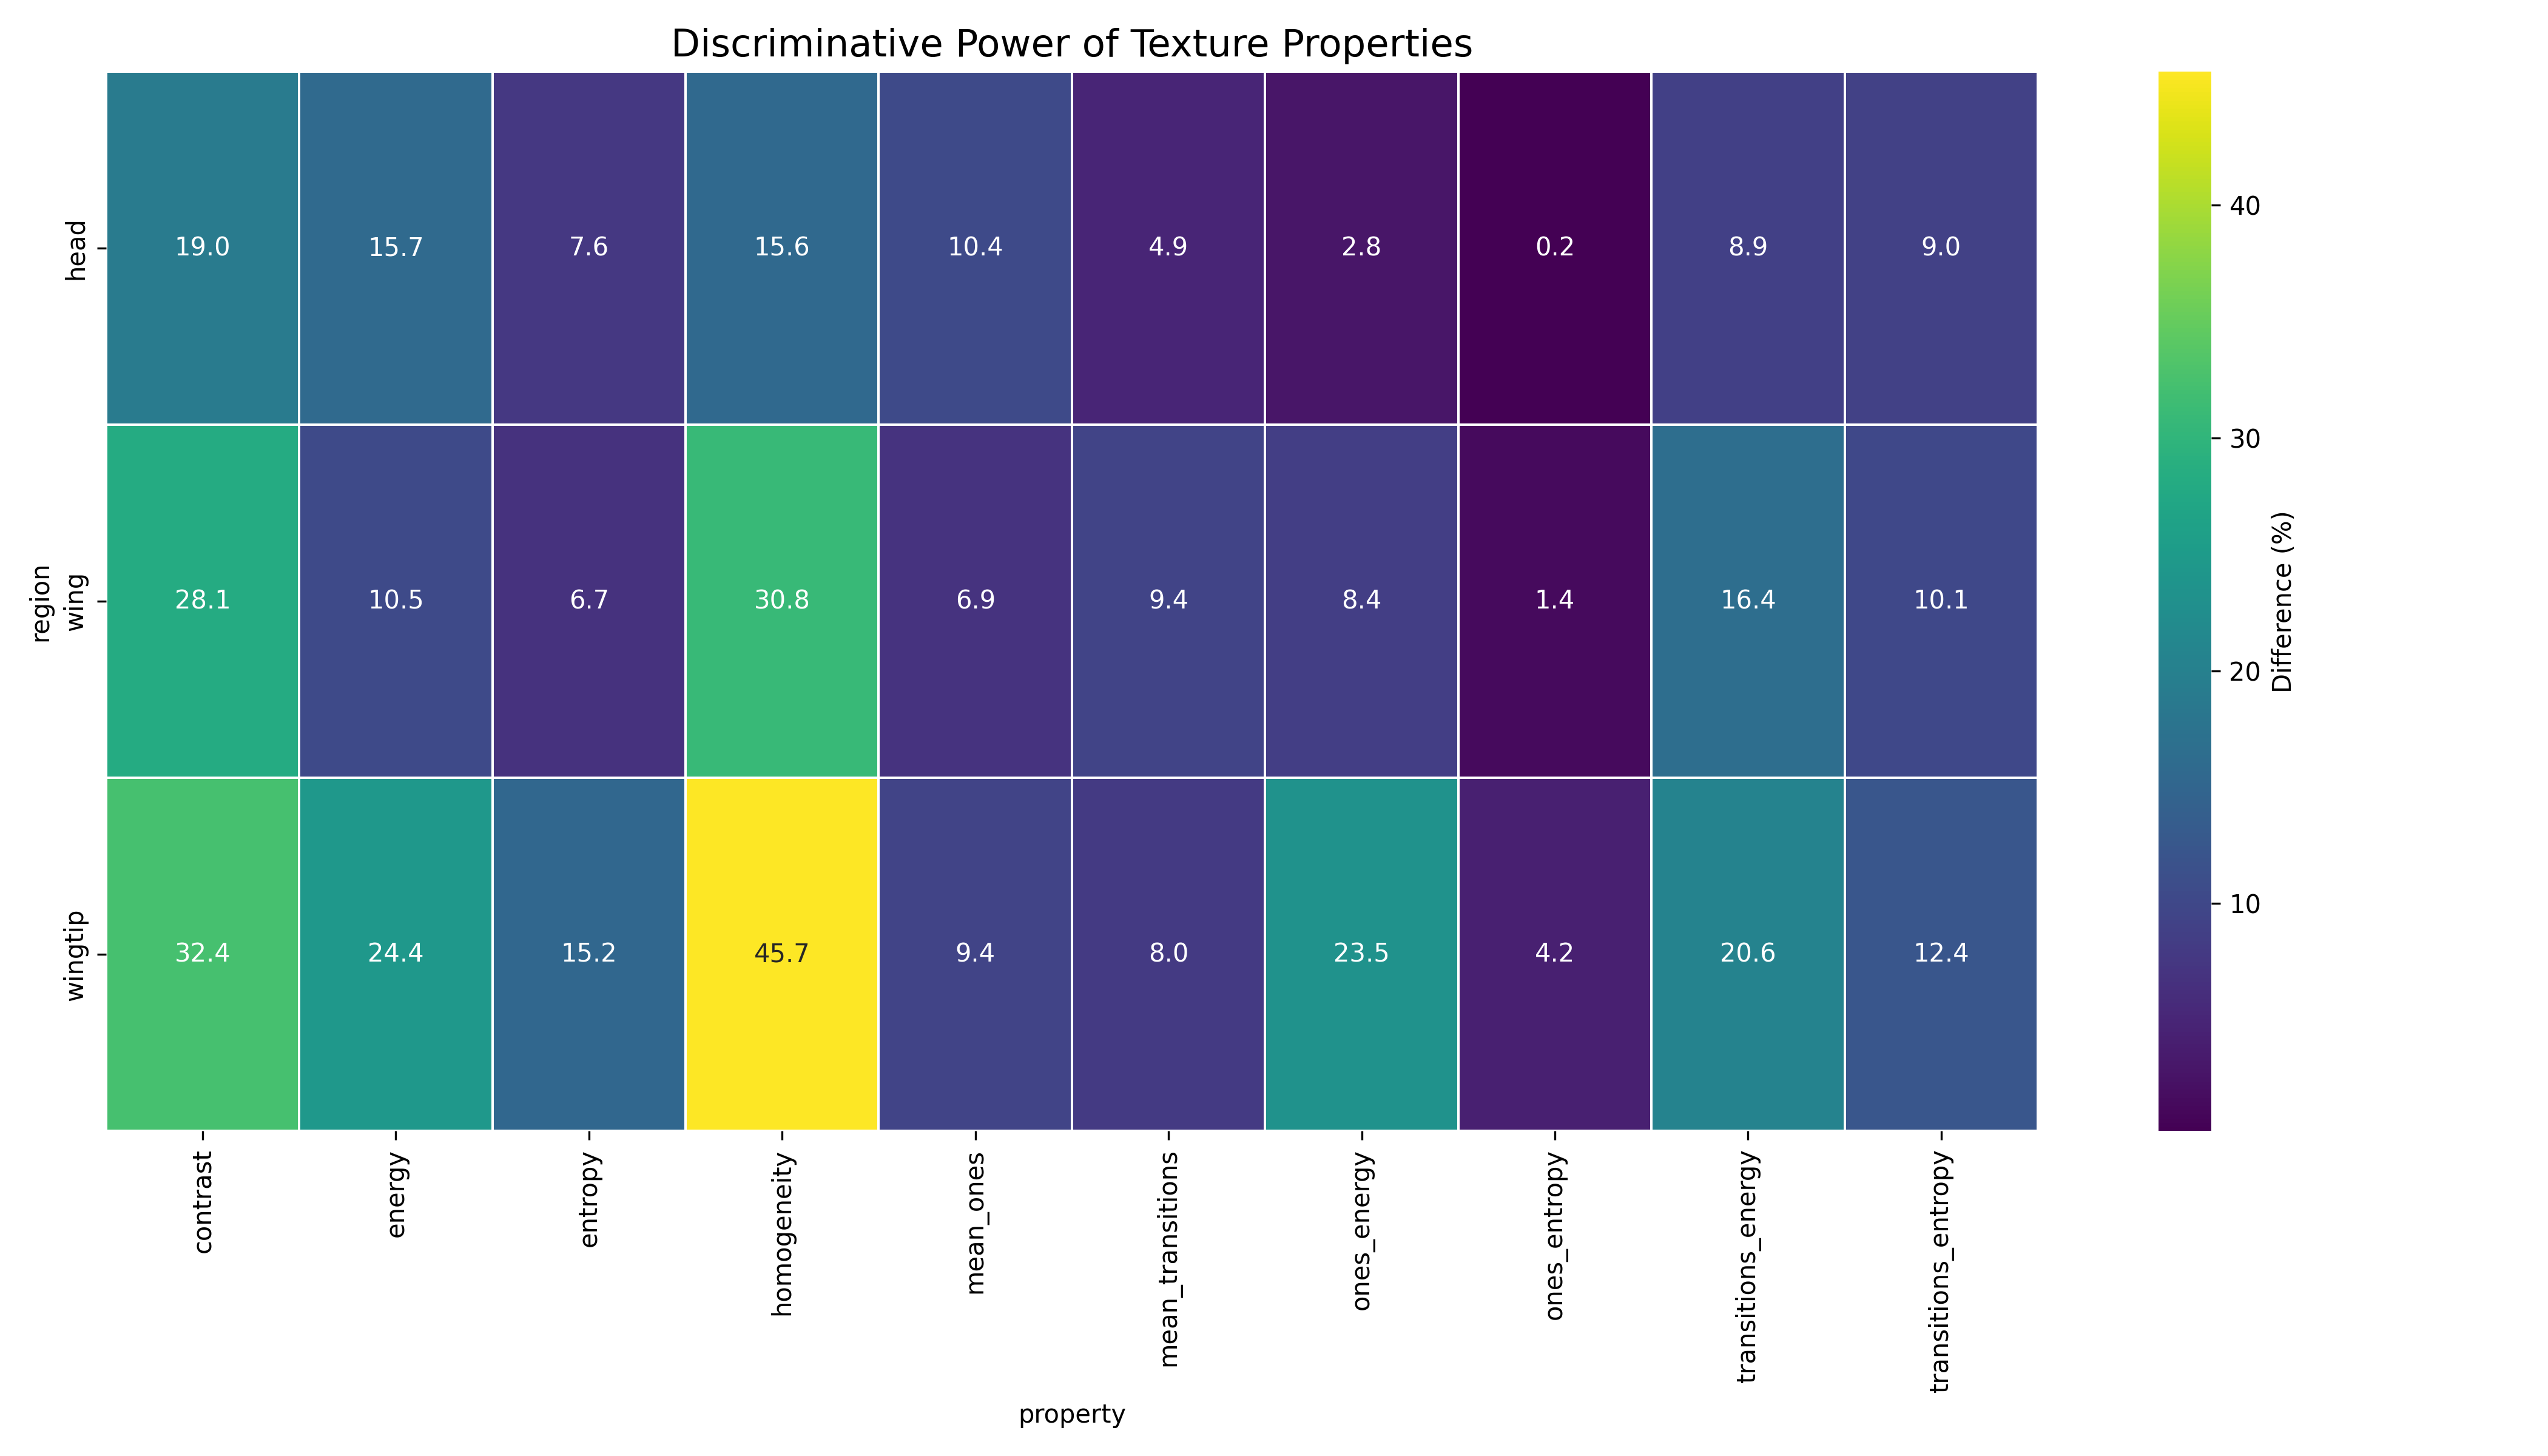
\includegraphics[width=\textwidth]{images/LBP/discriminative_power_heatmap.png}
        \caption{Regional discriminative power of texture properties}
        \label{fig:heatmap}
    \end{subfigure}
    \hfill
    \begin{subfigure}[b]{0.48\textwidth}
        \centering
        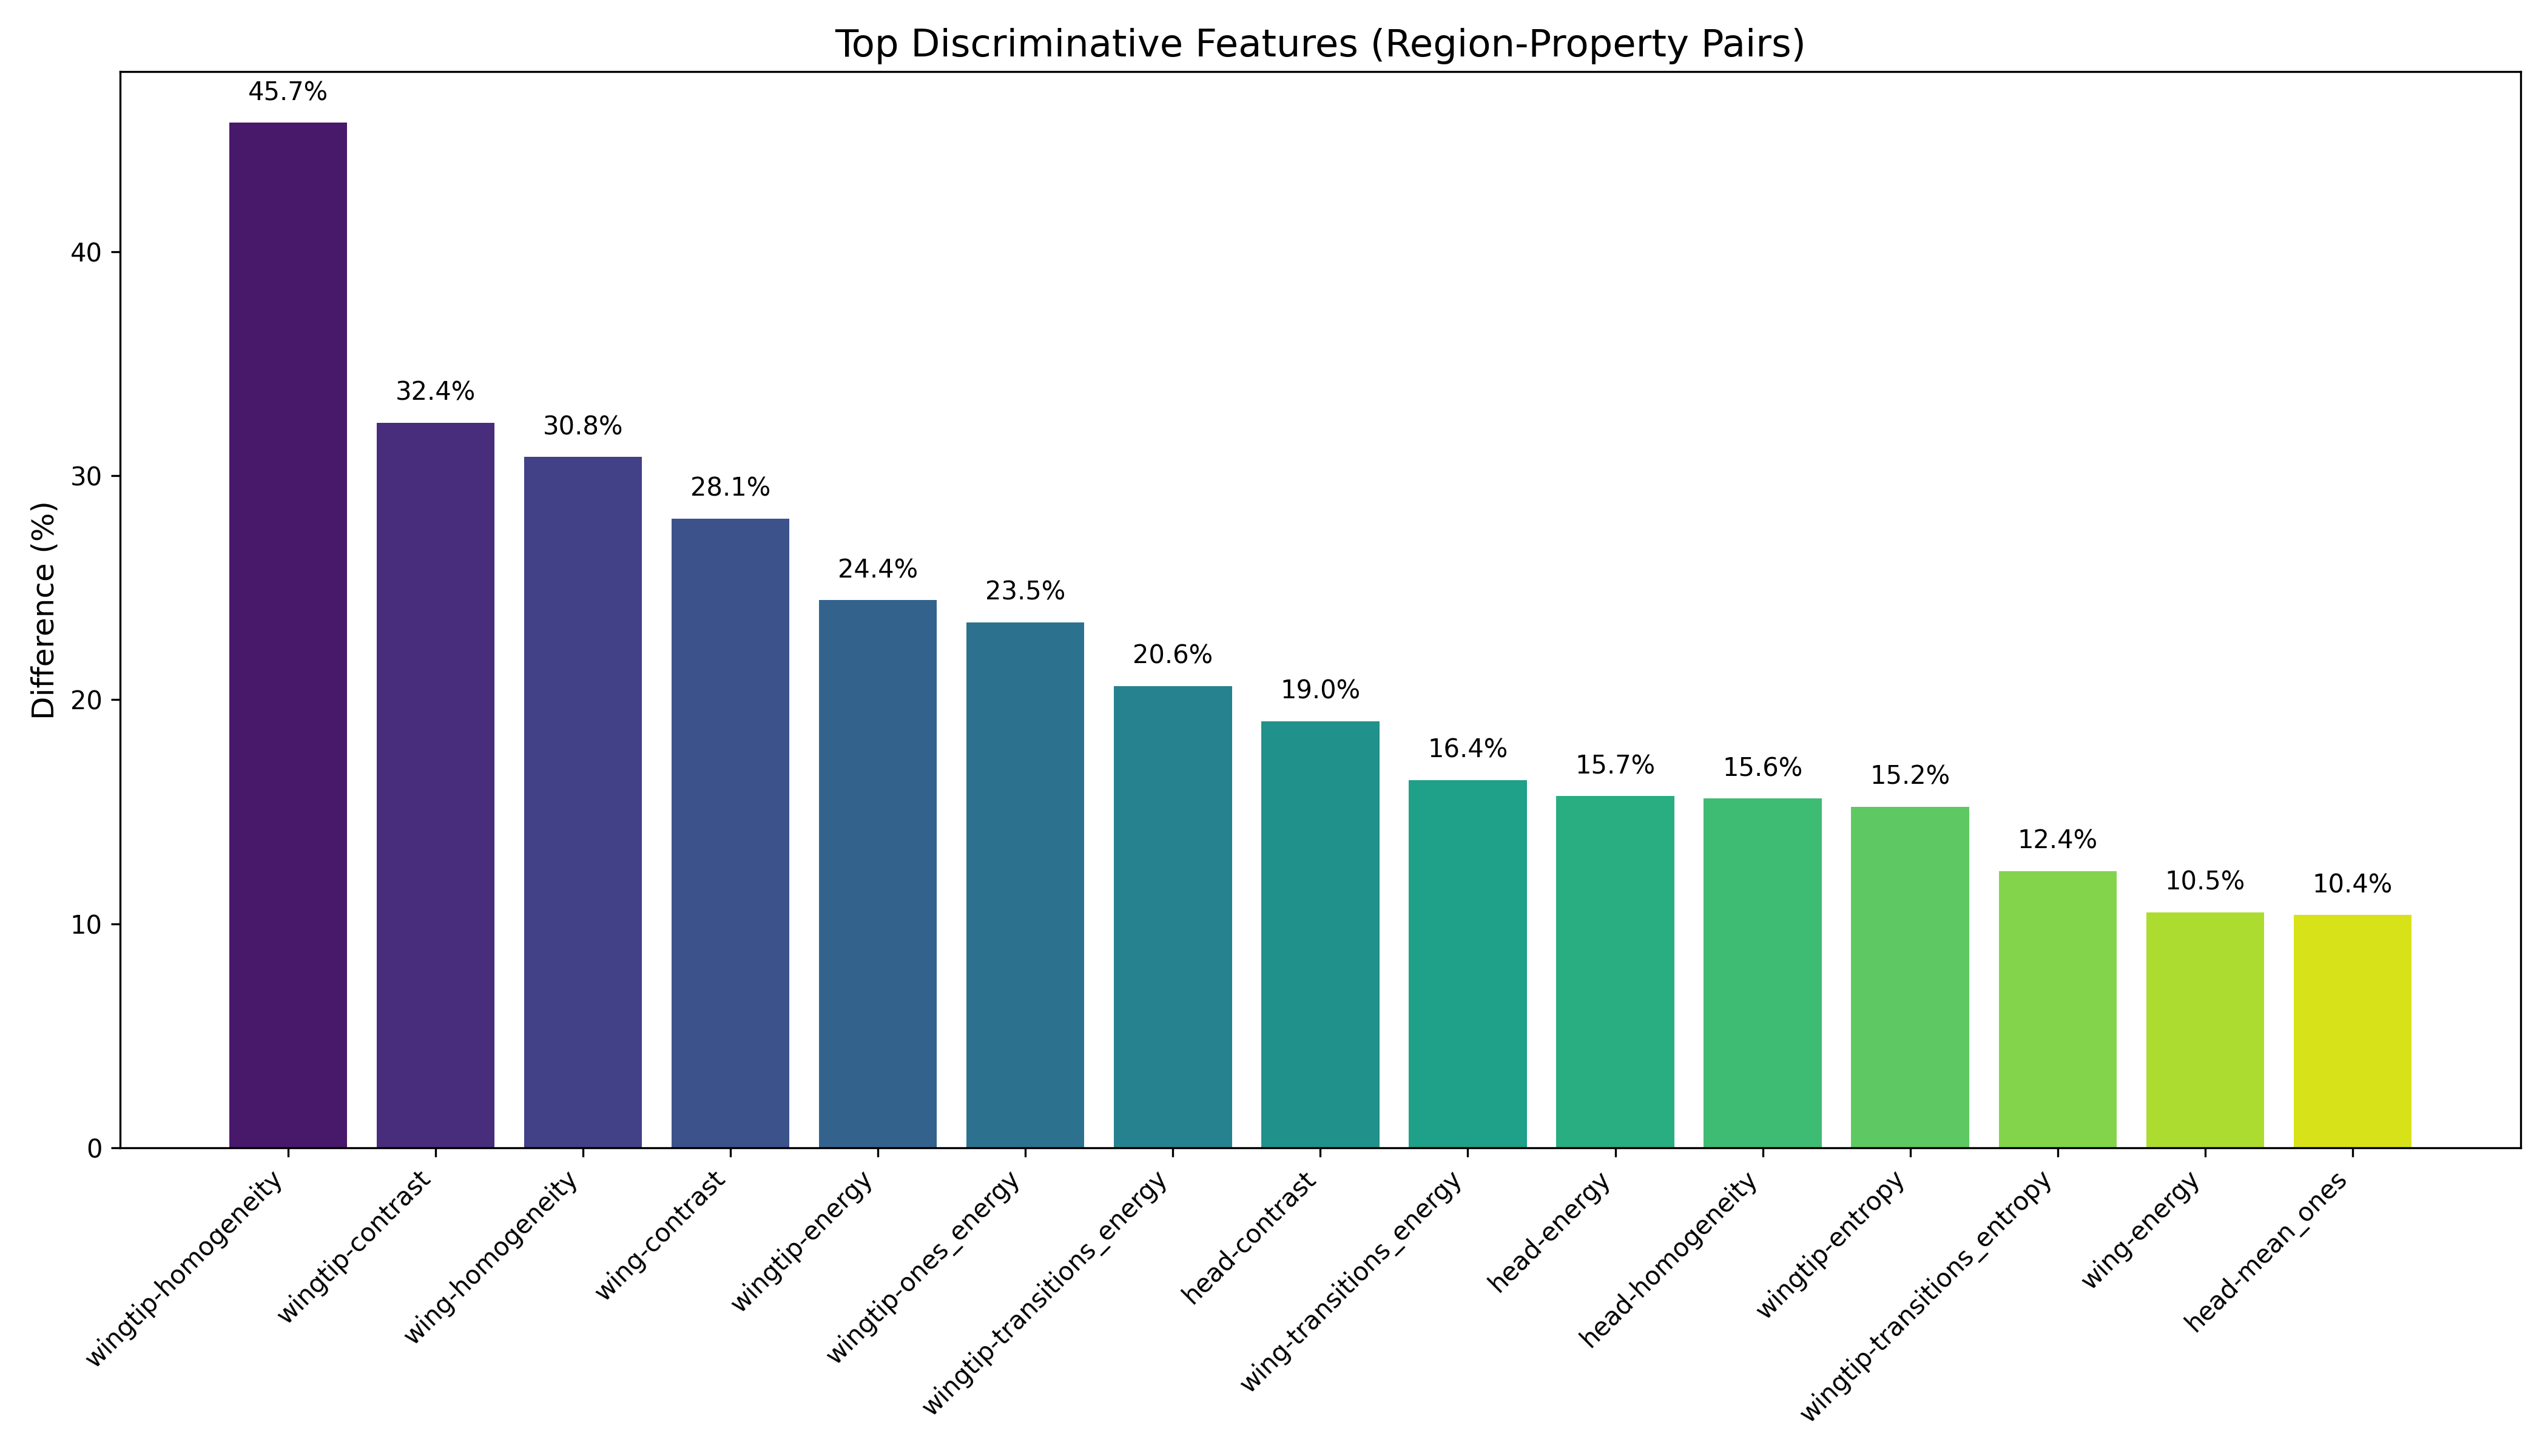
\includegraphics[width=\textwidth]{images/LBP/top_discriminative_features.png}
        \caption{Top discriminative features.}
        \label{fig:top_features}
    \end{subfigure}
    \caption{Discriminative power analysis of LBP texture features: (a) heatmap of regional differences, (b) top discriminative features.}
    \label{fig:lbp_discriminative_power}
\end{figure}

The discriminative power of LBP texture features is visualized as a heatmap and bar chart in Figure~\ref{fig:lbp_discriminative_power}, highlighting wingtip homogeneity (45.74\%), wingtip contrast (32.36\%), and wing homogeneity (30.83\%) as the top three discriminative features.

\subsection{Limitations of standard LBP code analysis}
\label{subsec:feature_limitations}

Although standard texture properties demonstrated substantial differences between species (with top feature close to 50\% difference), it is important to note that the features from LBP pattern codes are not guaranteed to be rotationally invariant. The abstract features (Number of Ones and Transitions) showed more modest discriminative power (maximum 10.4\%) but can be considered rotation variant since we are only dealing with the presence or count of ones or transitions in a region.

\begin{figure}[H]
    \centering
    \begin{subfigure}[b]{0.49\textwidth}
        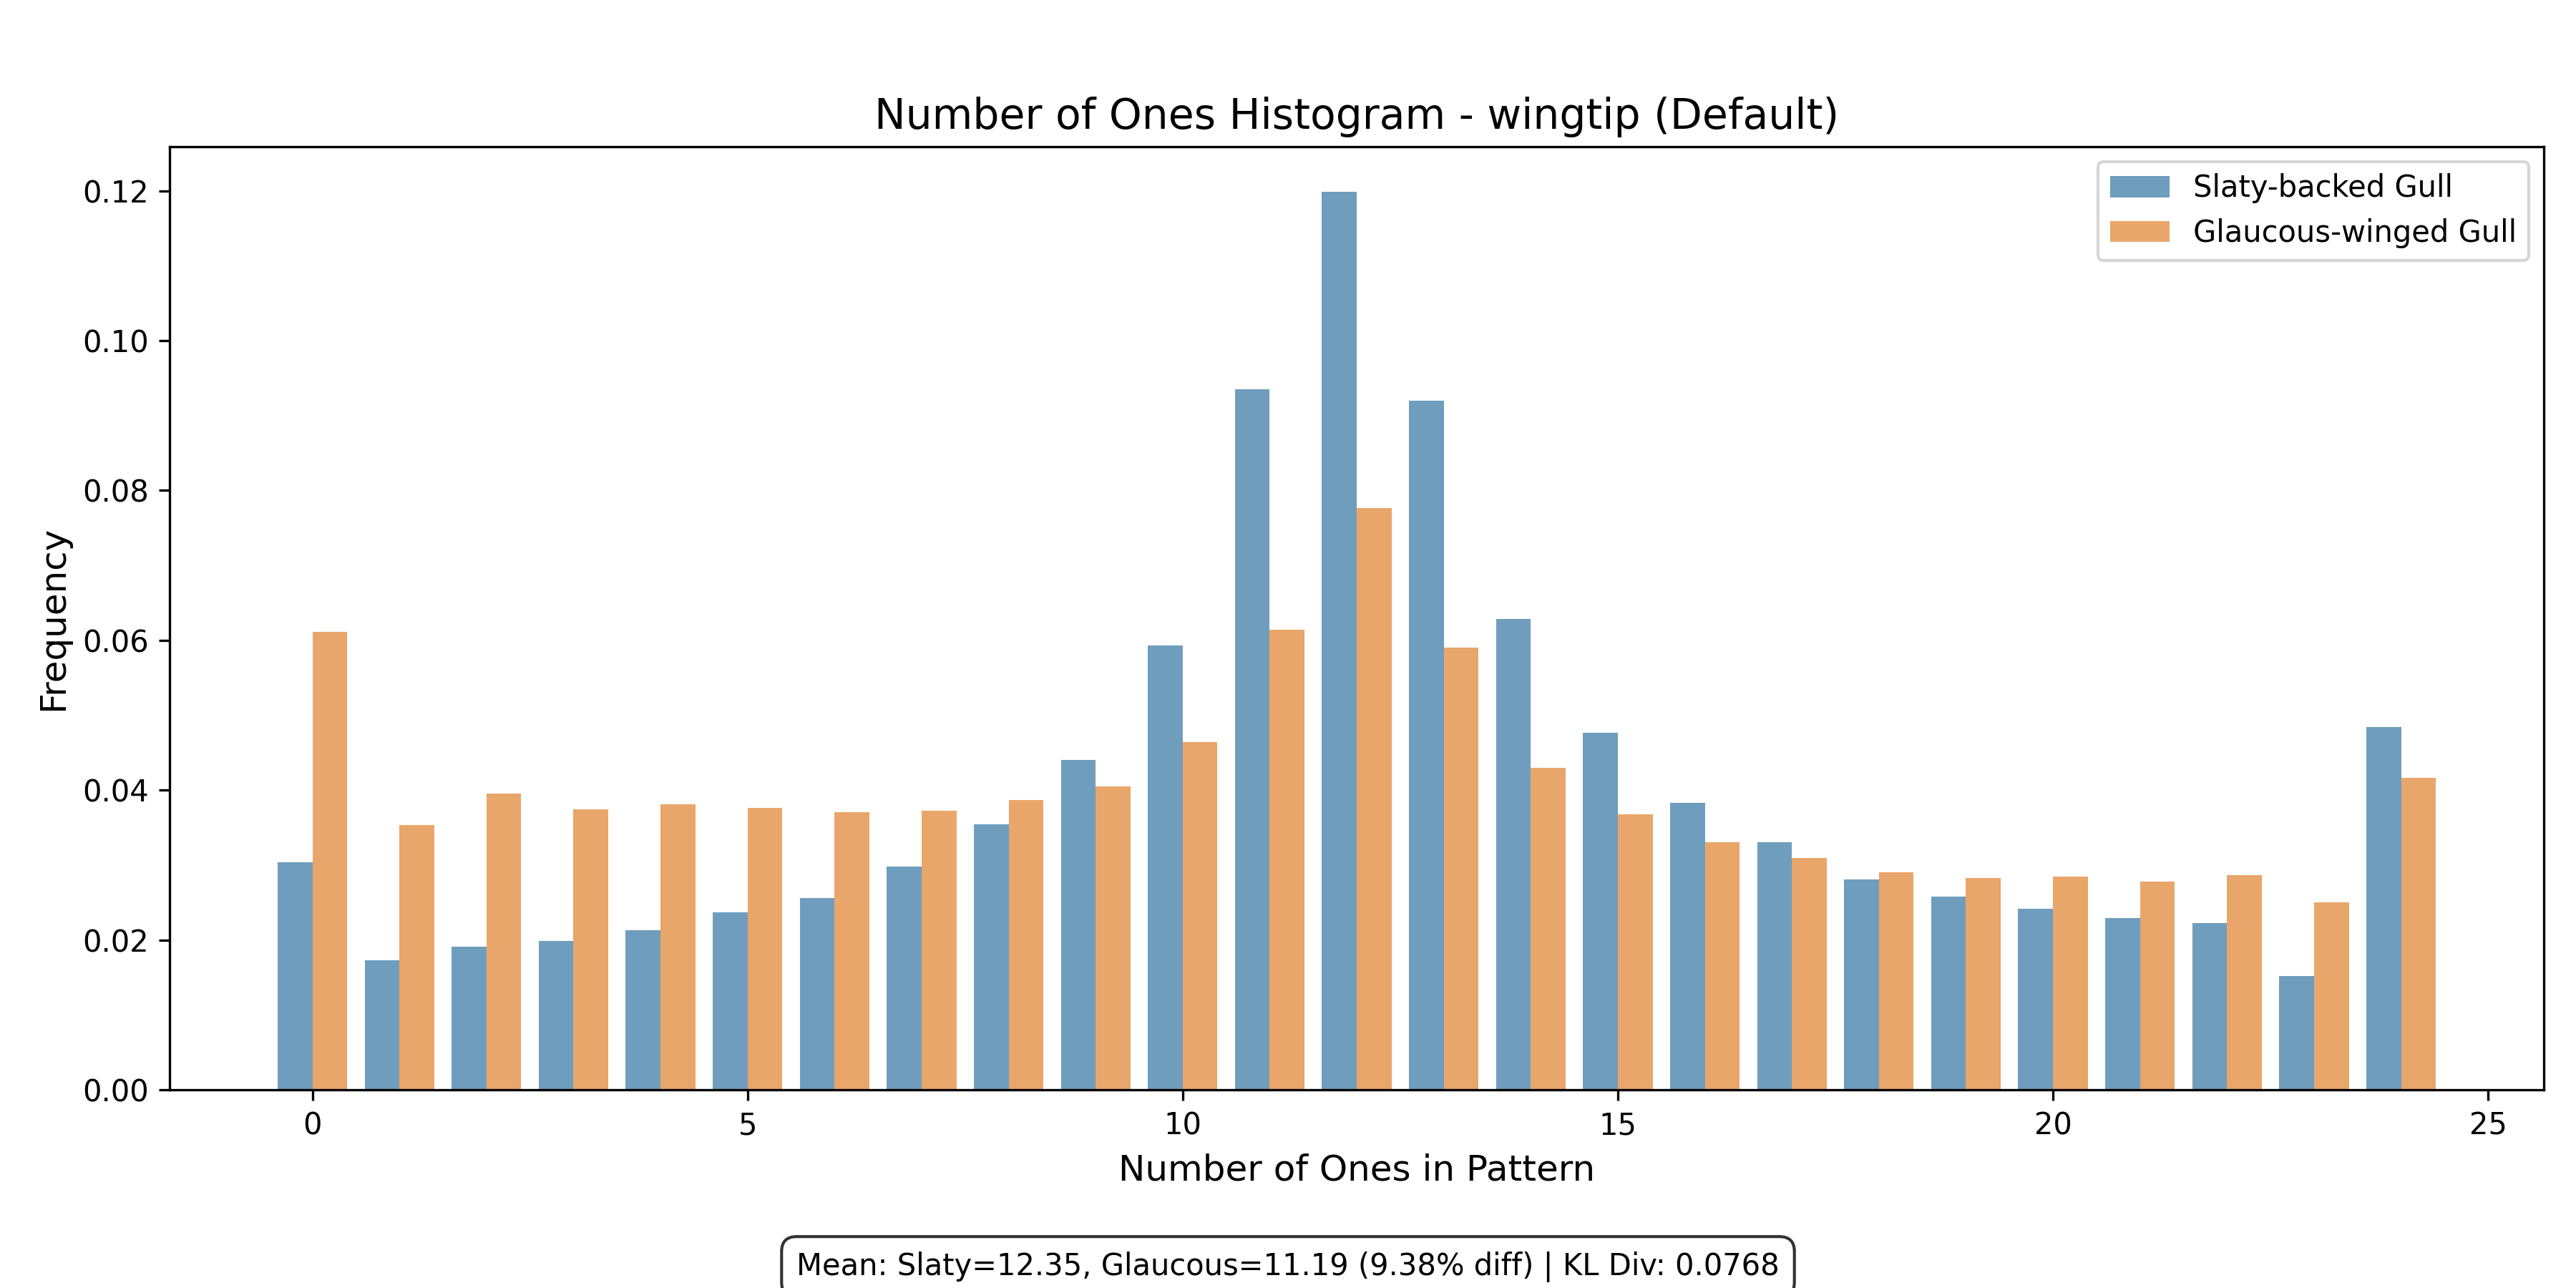
\includegraphics[width=\textwidth]{images/LBP/default_wingtip_ones_histogram.png}
        \caption{Wingtip Number of Ones distribution (9.38\% difference)}
        \label{fig:wingtip_ones}
    \end{subfigure}
    \hfill
    \begin{subfigure}[b]{0.49\textwidth}
        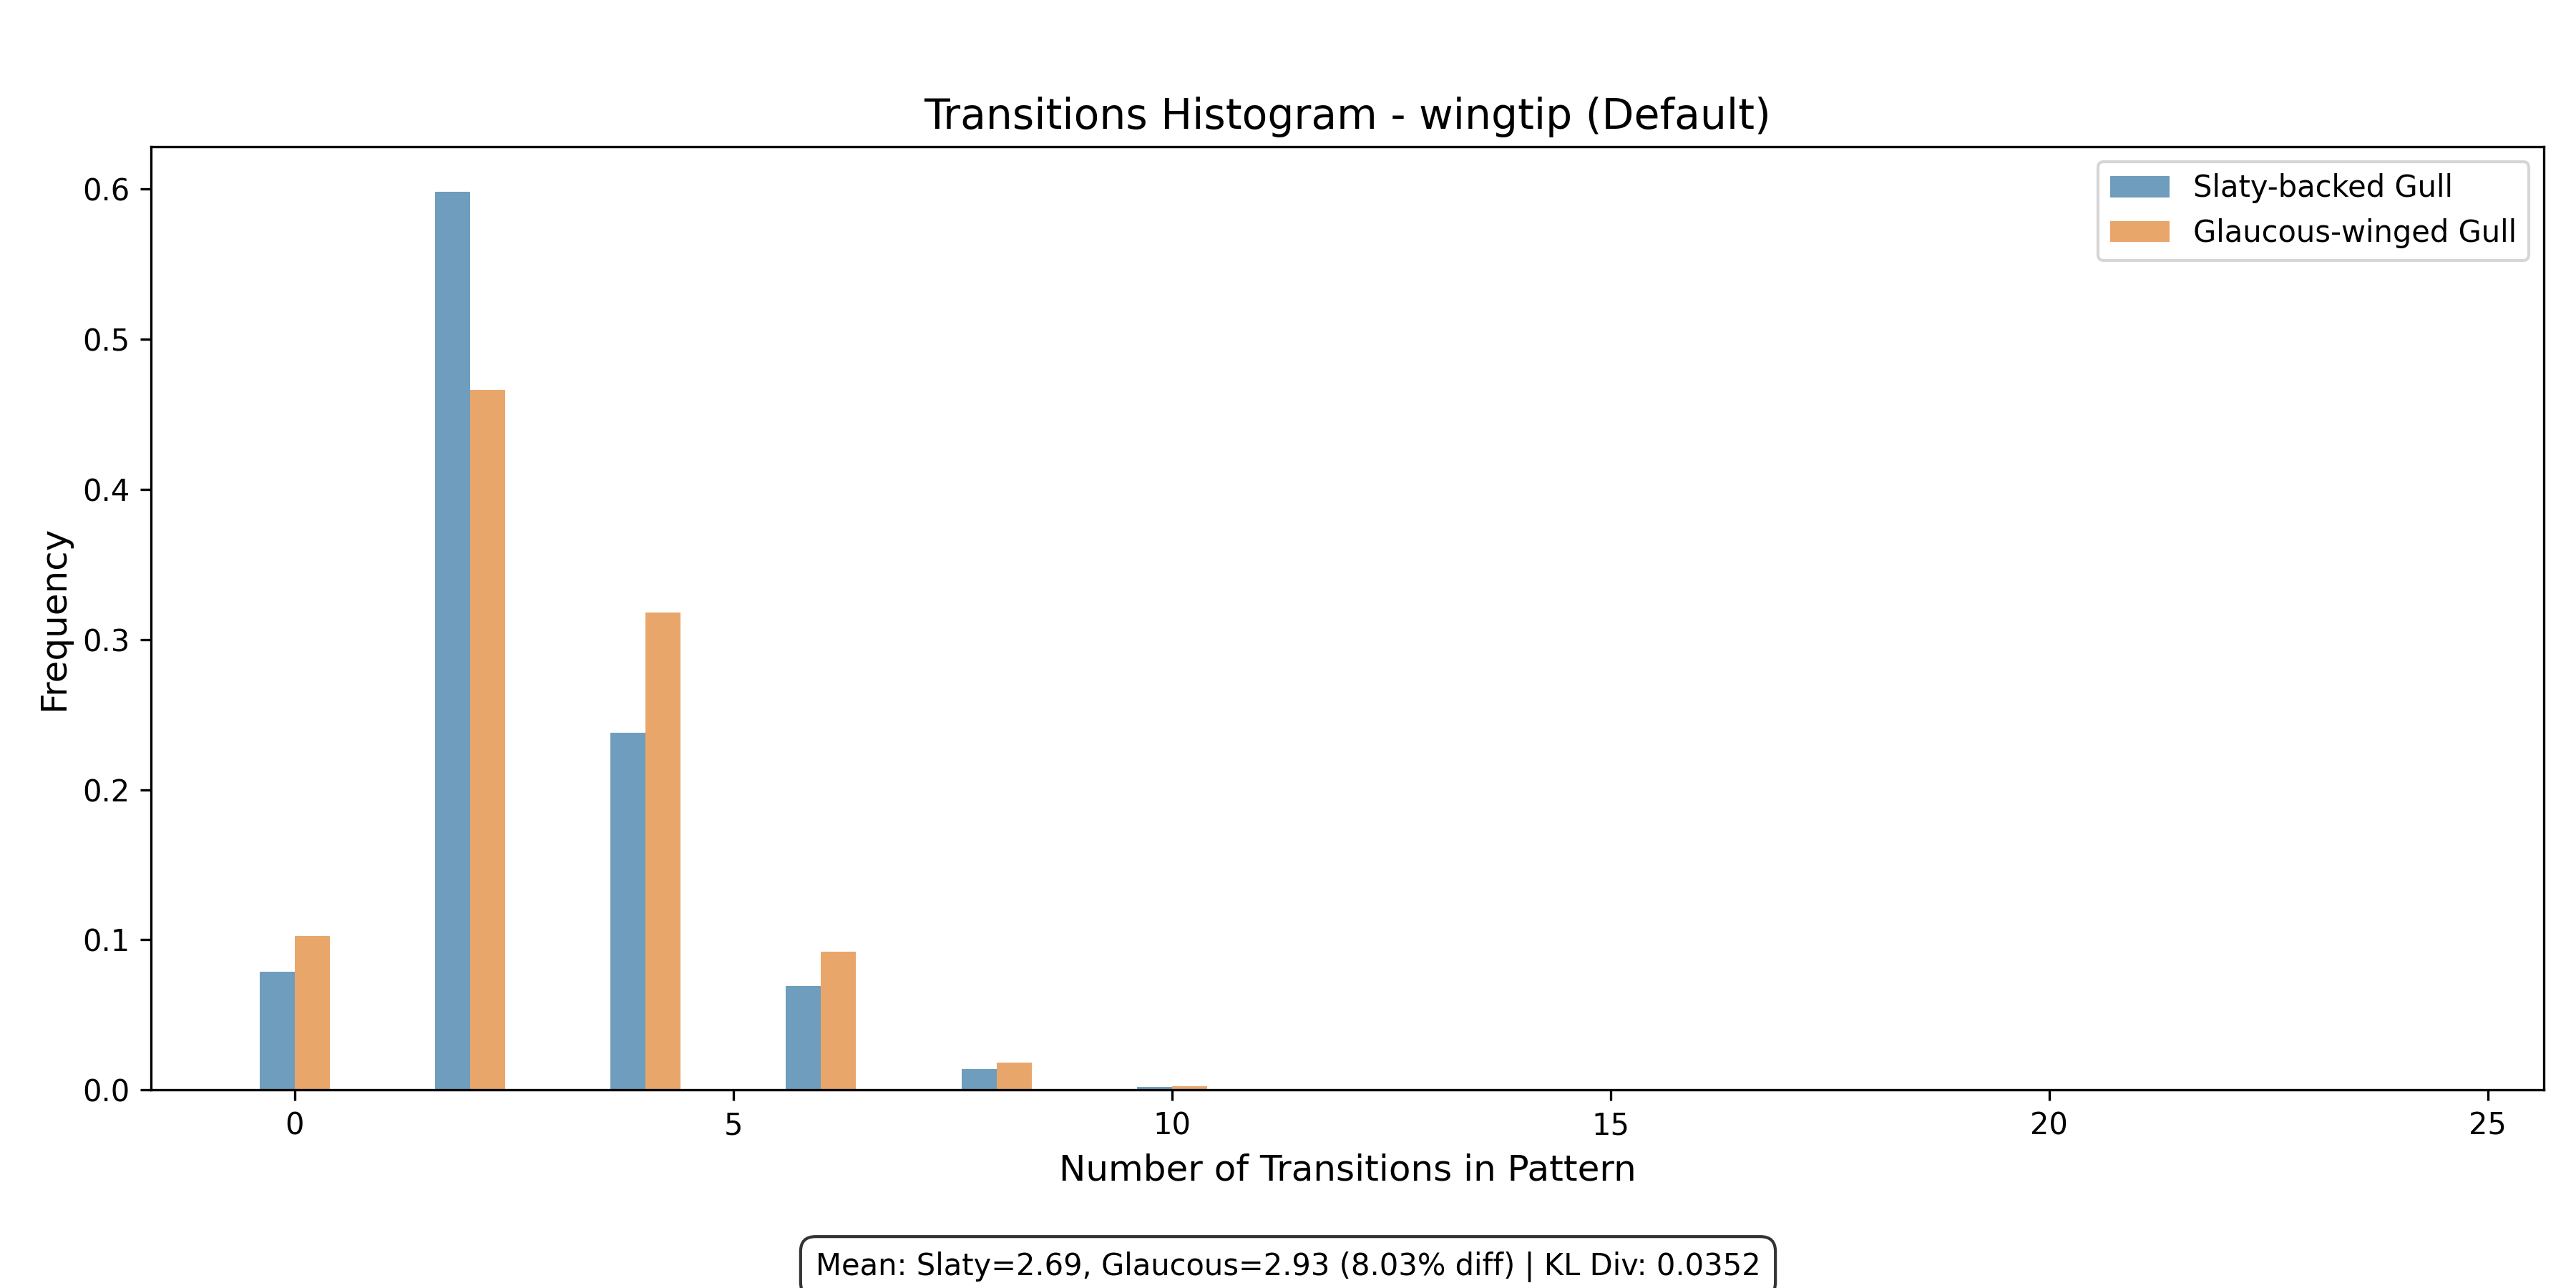
\includegraphics[width=\textwidth]{images/LBP/default_wingtip_transitions_histogram.png}
        \caption{Wingtip Transitions distribution (8.0\% difference)}
        \label{fig:wingtip_transitions}
    \end{subfigure}
    \caption{Histograms of LBP features for the wingtip region: (a) Number of Ones, (b) Transitions.}
    \label{fig:wingtip_feature_histograms}
\end{figure}

\begin{figure}[H]
    \centering
    \begin{subfigure}[b]{0.49\textwidth}
        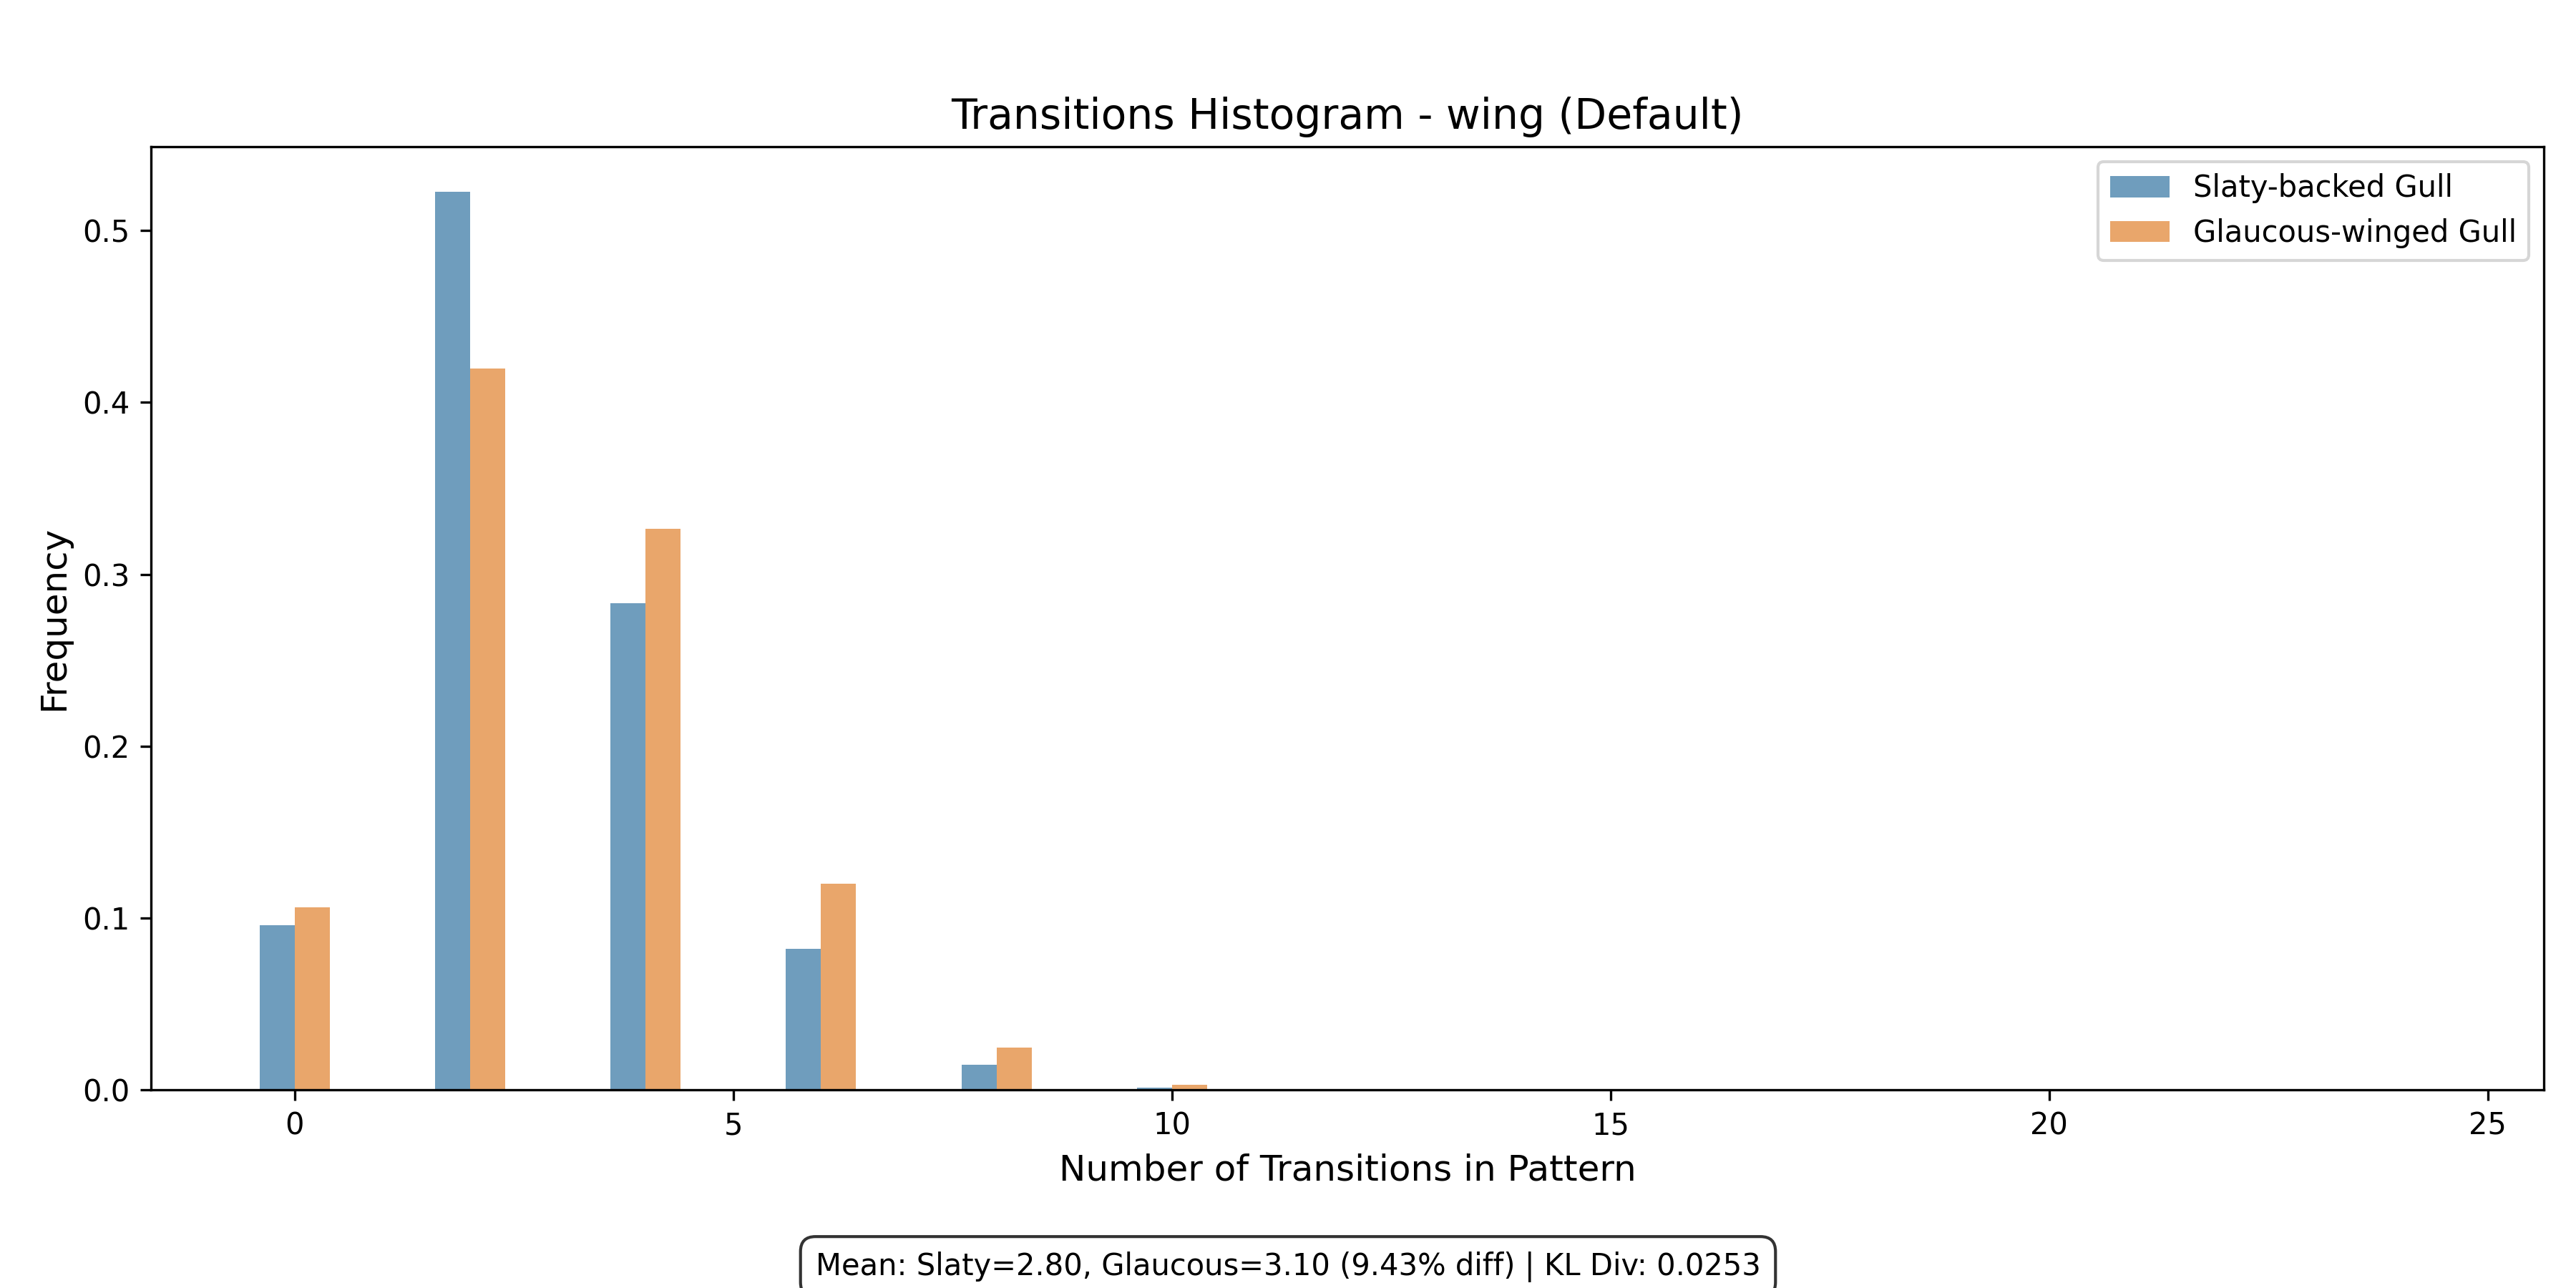
\includegraphics[width=\textwidth]{images/LBP/default_wing_transitions_histogram.png}
        \caption{Wing Transitions distribution (9.4\% difference)}
        \label{fig:wing_transitions}
    \end{subfigure}
    \hfill
    \begin{subfigure}[b]{0.49\textwidth}
        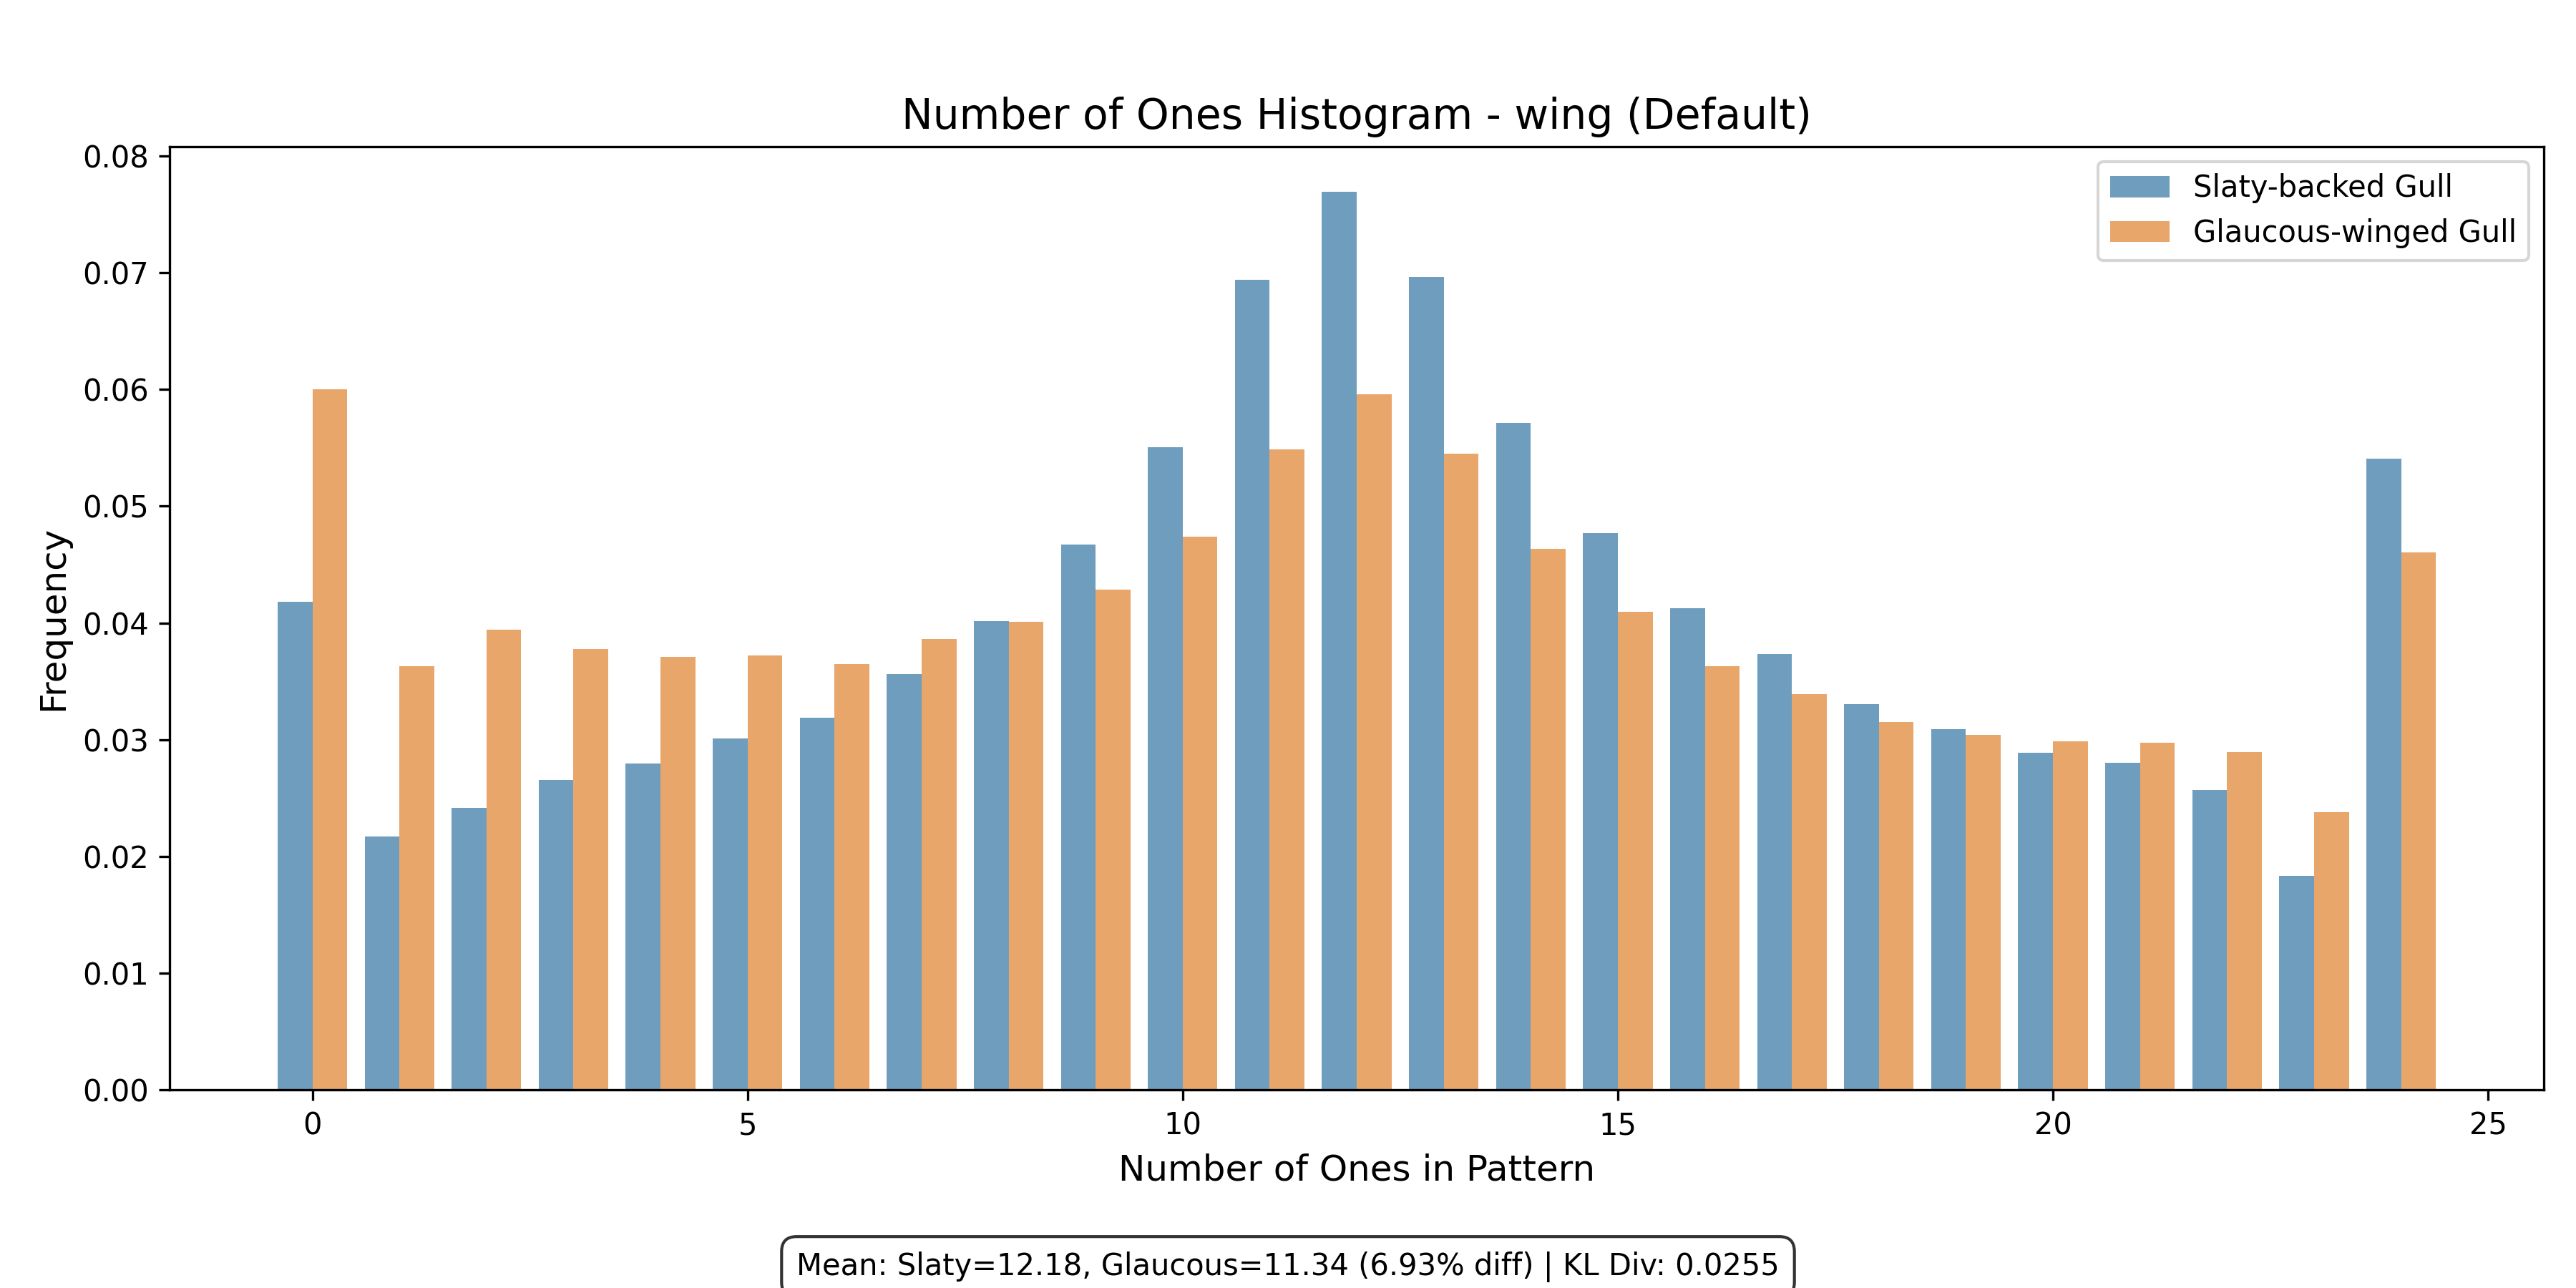
\includegraphics[width=\textwidth]{images/LBP/default_wing_ones_histogram.png}
        \caption{Wing Number of Ones distribution (7.5\% difference)}
        \label{fig:wing_ones}
    \end{subfigure}
    \caption{Histograms of LBP features for the wing region: (a) Transitions, (b) Number of Ones.}
    \label{fig:wing_feature_histograms}
\end{figure}

The distributions of the 'Number of Ones' and 'Transitions' features for the wingtip and wing regions are shown as histograms in Figures~\ref{fig:wingtip_feature_histograms} and~\ref{fig:wing_feature_histograms}, respectively.

\subsection{Abstract Feature Distributions}
\begin{figure}[H]
    \centering
    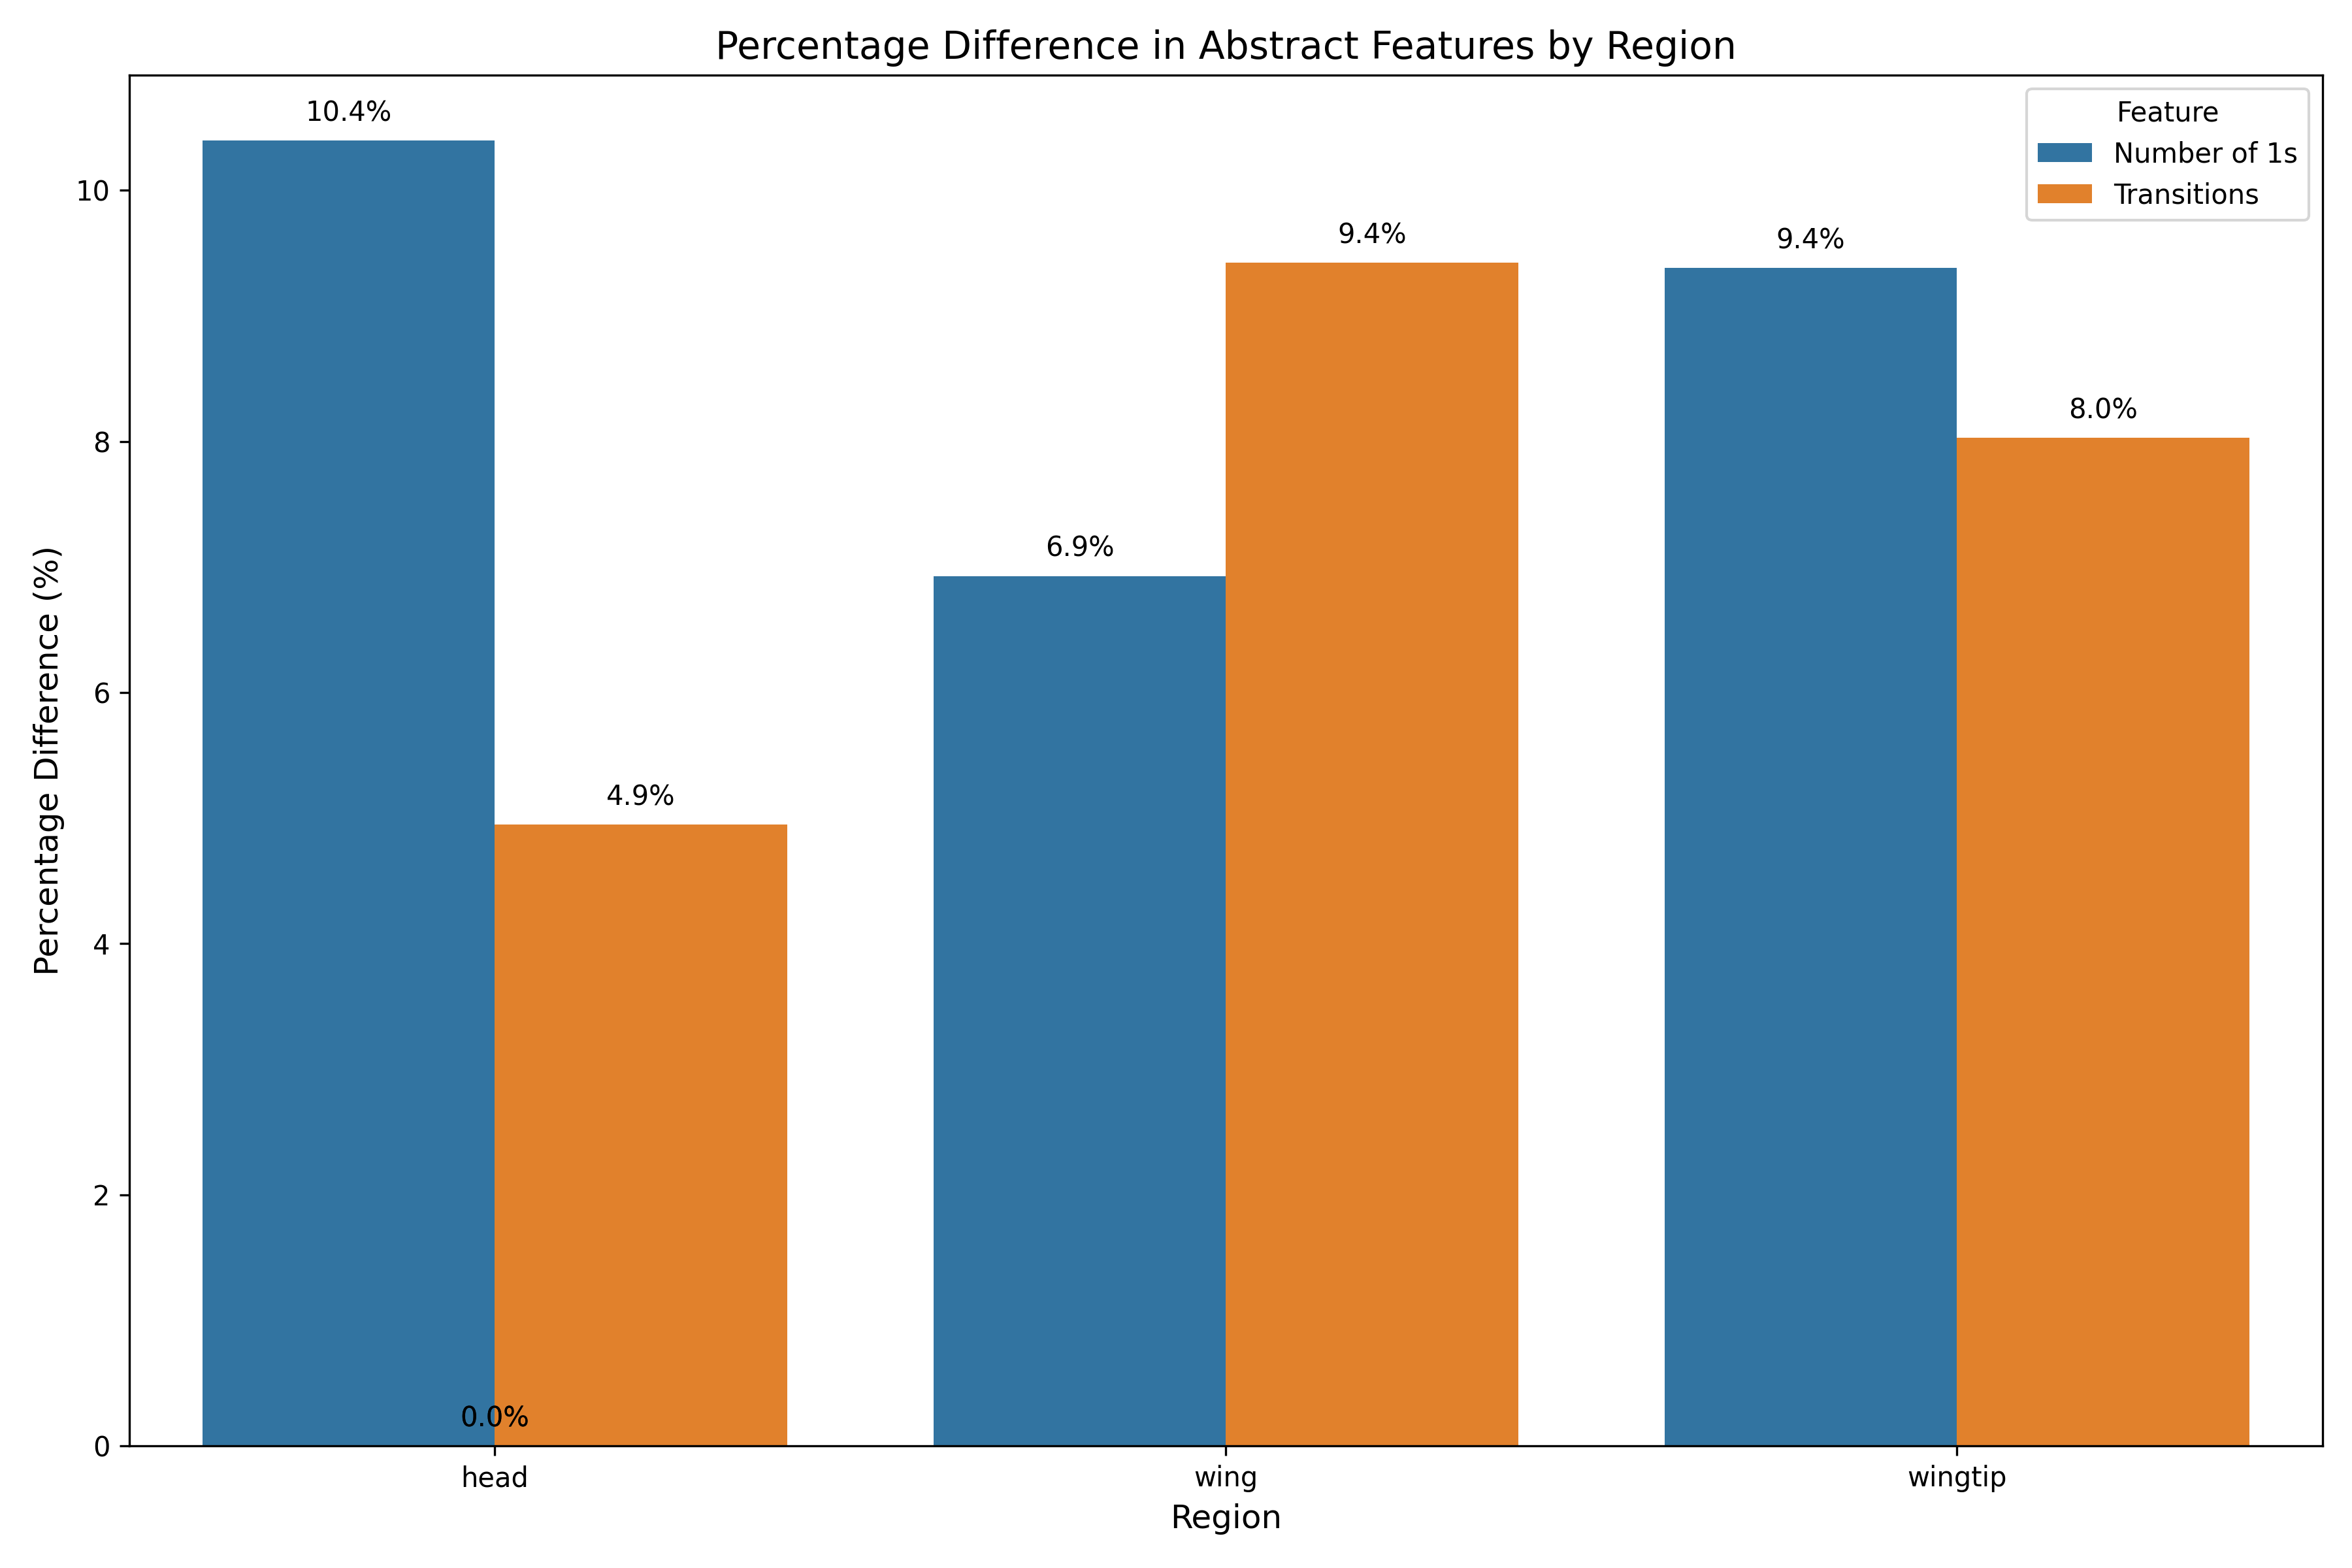
\includegraphics[width=0.38\textwidth]{images/LBP/default_feature_diff_barchart.png}
    \caption{Abstract feature differences, showing head region's Number of Ones as most discriminative (10.4\% difference).}
    \label{fig:abstract_features}
\end{figure}

The figures illustrate the results of abstract features across different regions. Figure~\ref{fig:abstract_features} presents a bar chart highlighting the most discriminative feature from 1s and transitions histogram, showcasing their respective differences.

\subsection{Top Discriminative Features from 1s and Transitions Histograms}
\begin{table}[H]
    \centering
    \caption{Top discriminative region-histogram features ranked by percentage difference.}
    \label{tab:region_histogram_features}
    \begin{tabular}{c c c c c}
        \toprule
        \textbf{Rank} & \textbf{Region} & \textbf{Histogram Feature} & \textbf{Statistic} & \textbf{Difference (\%)} \\
        \midrule
        1 & Wingtip & Ones & Energy & 23.5 \\
        2 & Wingtip & Transitions & Energy & 20.6 \\
        3 & Wing & Transitions & Energy & 16.4 \\
        \bottomrule
    \end{tabular}   
    \label{tab:top_discriminative_features}
\end{table}

To further quantify these observations and analyse the texture features calculated from the histograms, Table~\ref{tab:top_discriminative_features} lists the top discriminative features based on their percentage differences between species. The analysis demonstrates that LBP texture features, particularly in the wingtip and wing region, can provide robust discriminative power for gull species identification although the difference is very small.

\section{Clustering Results}

\subsection{Clustering Performance Metrics}

The performance of each clustering algorithm was evaluated using both unsupervised and supervised metrics. Table~\ref{tab:clustering_metrics} presents a comprehensive comparison of the three clustering approaches.

\begin{table}[H]
    \centering
    \caption{Performance and confusion matrix summary for clustering algorithms. TP = True Positives, FN = False Negatives, GWG = Glaucous-Winged Gull, SBG = Slaty-Backed Gull.}
    \label{tab:clustering_metrics}
    \resizebox{\textwidth}{!}{%
    \begin{tabular}{lcccccccc}
    \toprule
    \textbf{Algorithm} & \textbf{Silhouette} & \textbf{ARI} & \textbf{Accuracy} & \textbf{TP (GWG)} & \textbf{FN (GWG)} & \textbf{TP (SBG)} & \textbf{FN (SBG)} \\
    \midrule
    K-means      & 0.605 & 0.843 & 95.94\% & 88 & 5 & 101 & 3 \\
    Hierarchical & 0.594 & 0.881 & 96.95\% & 92 & 1 & 99 & 5 \\
    GMM          & 0.548 & 0.717 & 92.39\% & 78 & 15 & 104 & 0 \\
    \bottomrule
    \end{tabular}
    }
\end{table}

Table~\ref{tab:clustering_metrics} summarizes the key performance metrics and confusion matrix results for all three clustering algorithms. The silhouette score (ranging from -1 to 1) measures how well-separated the clusters are, with higher values indicating better-defined clusters. The Adjusted Rand Index (ARI) measures the similarity between the clustering results and the ground truth labels, with values closer to 1 indicating better alignment with the actual species classification.

% \begin{figure}[H]
%     \centering
%     \includegraphics[width=0.8\textwidth]{images/clustering/feature_importance.png}
%     \caption{Feature importance based on absolute differences between cluster centers, highlighting the most discriminative features for species classification.}
%     \label{fig:feature_importance}
% \end{figure}

The prominence of wing intensity features aligns with ornithological knowledge that Slaty-Backed Gulls typically exhibit darker wing patterns compared to Glaucous-Winged Gulls, providing a data-driven validation of these distinguishing characteristics.

\subsection{Integration with Visual Analysis}

The clustering performance is visualized through two complementary perspectives: the cluster formations in reduced PCA space and the classification accuracy via confusion matrices considering majorily class to be the true class of the cluster.
Figure~\ref{fig:cluster_visualizations} demonstrates how each clustering algorithm partitions the data in the PCA-reduced feature space. The K-means visualization (Figure~\ref{fig:kmeans_cluster}) clearly shows two well-defined clusters with distinct centroids, while hierarchical clustering (Figure~\ref{fig:hierarchical_cluster}) exhibits similar separation but with slightly different cluster boundaries. The GMM results (Figure~\ref{fig:gmm_cluster}) show more density-based partitioning that accommodates the natural distribution of the data points.


\begin{figure}[H]
    \centering
    \begin{subfigure}[b]{0.32\textwidth}
        \centering
        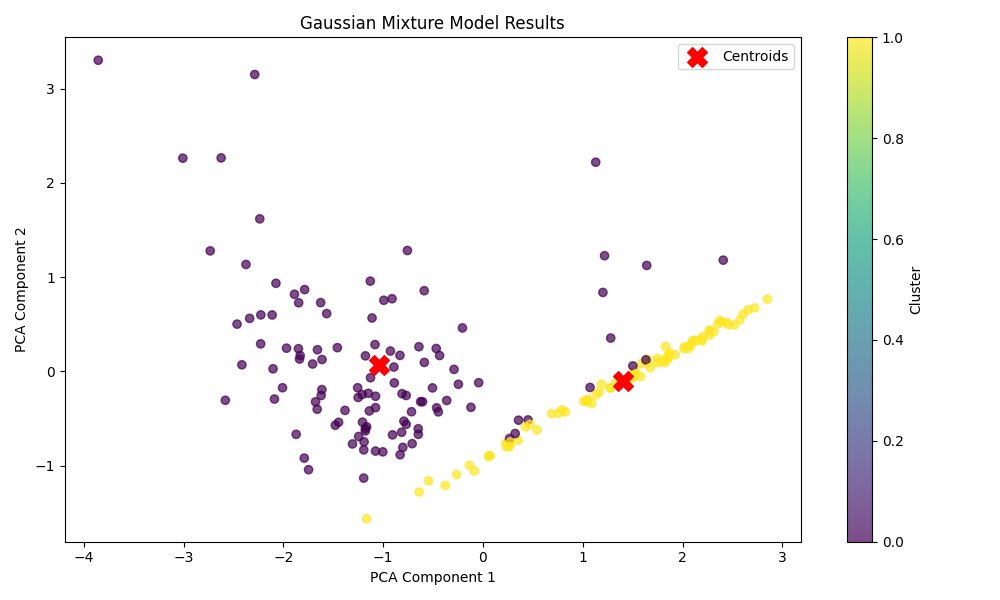
\includegraphics[width=\textwidth]{images/clustering/gmm_clustering.png}
        \caption{GMM Clustering}
        \label{fig:gmm_cluster}
    \end{subfigure}
    \hfill
    \begin{subfigure}[b]{0.32\textwidth}
        \centering
        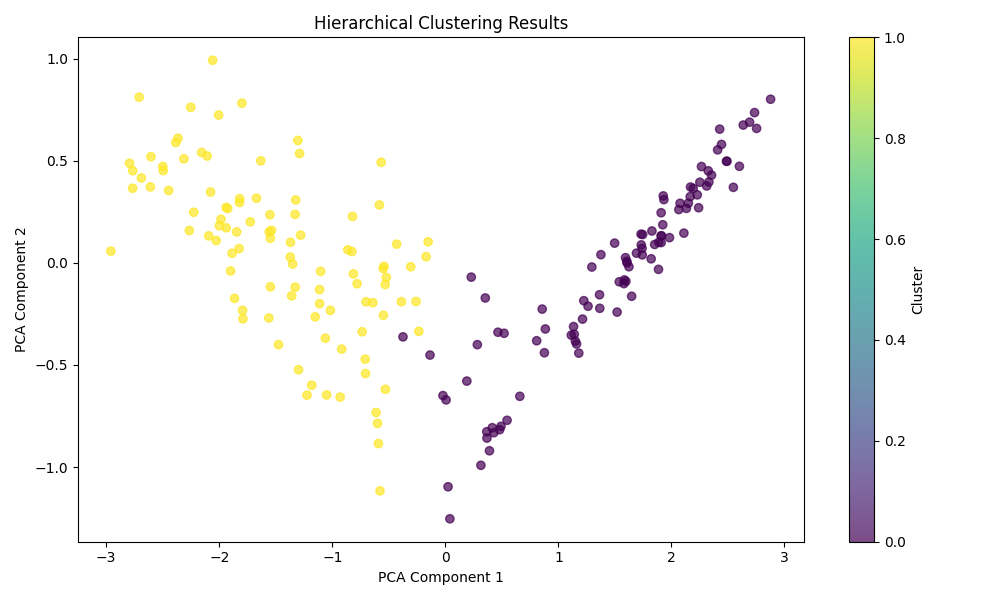
\includegraphics[width=\textwidth]{images/clustering/hierarchical_clustering.png}
        \caption{Hierarchical}
        \label{fig:hierarchical_cluster}
    \end{subfigure}
    \hfill
    \begin{subfigure}[b]{0.32\textwidth}
        \centering
        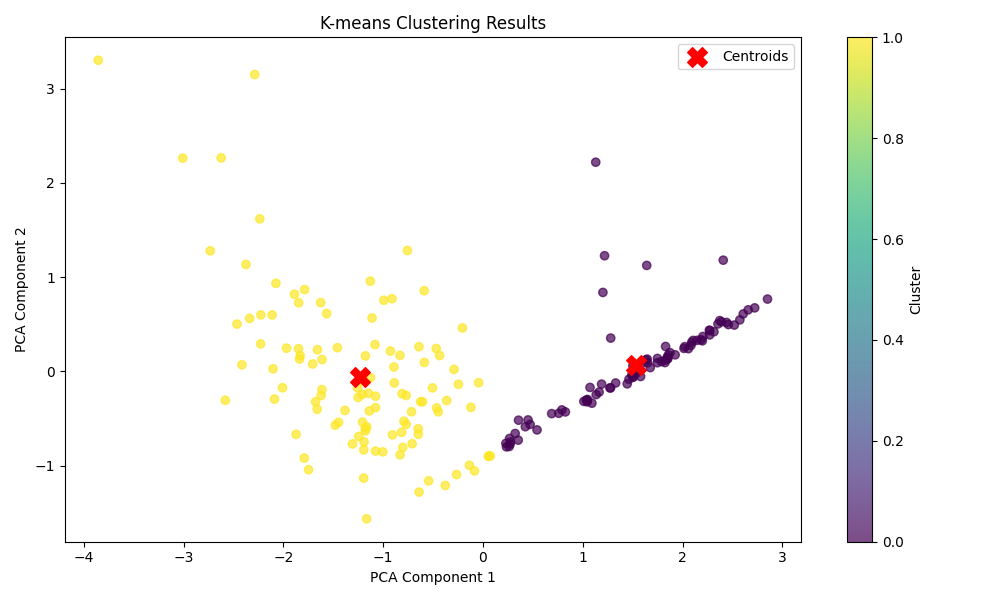
\includegraphics[width=\textwidth]{images/clustering/kmeans_clustering.png}
        \caption{K-means}
        \label{fig:kmeans_cluster}
    \end{subfigure}
    \caption{Cluster formations in PCA-reduced space showing the distribution of data points with centroids marked for K-means and GMM. All three algorithms show clear separation between the two species along PCA Component 1.}
    \label{fig:cluster_visualizations}
\end{figure}

\begin{figure}[H]
    \centering
    \begin{subfigure}[b]{0.32\textwidth}
        \centering
        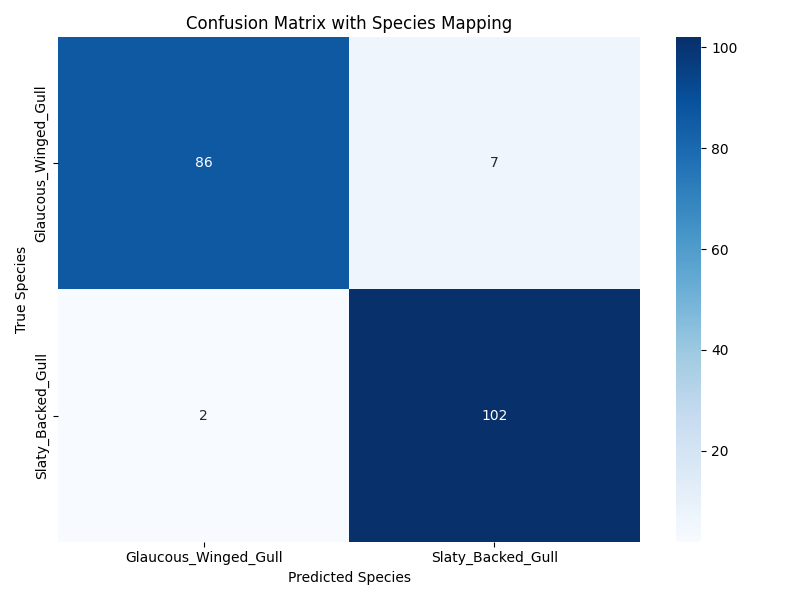
\includegraphics[width=\textwidth]{images/clustering/kmeans_confusion_matrix.png}
        \caption{K-means (Accuracy: 95.94\%)}
        \label{fig:kmeans_cm}
    \end{subfigure}
    \hfill
    \begin{subfigure}[b]{0.32\textwidth}
        \centering
        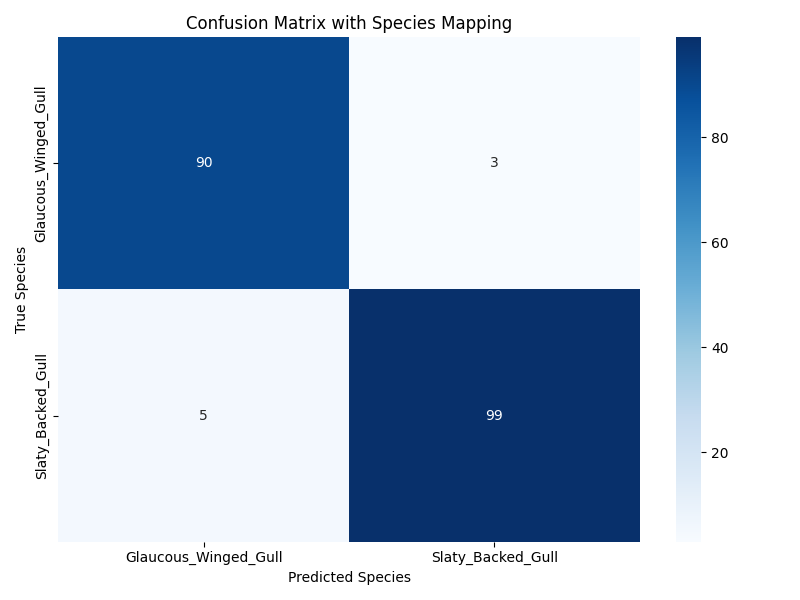
\includegraphics[width=\textwidth]{images/clustering/hierarchical_confusion_matrix.png}
        \caption{Hierarchical (Accuracy: 96.95\%)}
        \label{fig:hierarchical_cm}
    \end{subfigure}
    \hfill
    \begin{subfigure}[b]{0.32\textwidth}
        \centering
        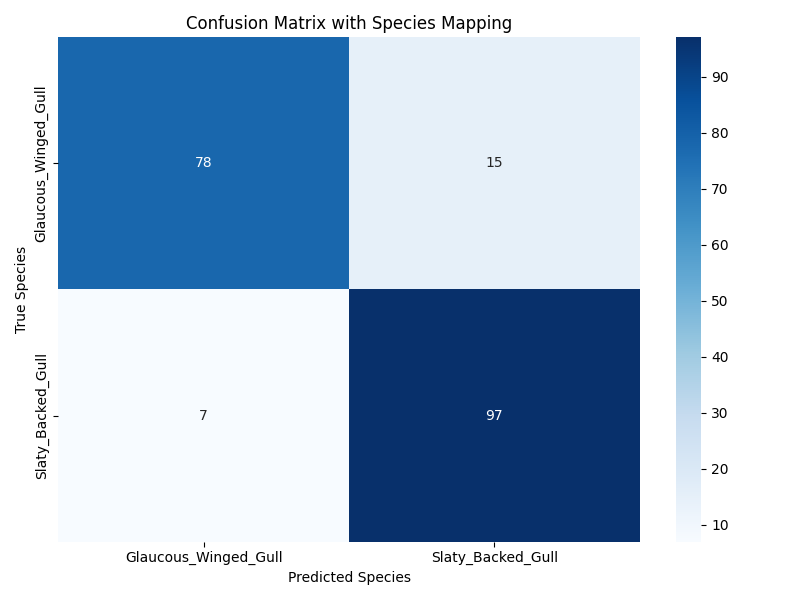
\includegraphics[width=\textwidth]{images/clustering/gmm_confusion_matrix.png}
        \caption{GMM (Accuracy: 92.39\%)}
        \label{fig:gmm_cm}
    \end{subfigure}
    \caption{Comparative confusion matrices showing classification performance across clustering algorithms, with hierarchical clustering achieving the highest overall accuracy.}
    \label{fig:confusion_matrices}
\end{figure}

The confusion matrices in Figure~\ref{fig:confusion_matrices} provide detailed insights into each algorithm's classification performance. The hierarchical clustering matrix (Figure~\ref{fig:hierarchical_cm}) shows excellent classification of Glaucous-Winged Gulls with only 1 false negative, while K-means (Figure~\ref{fig:kmeans_cm}) shows balanced performance across both species. The GMM confusion matrix (Figure~\ref{fig:gmm_cm}) reveals perfect recall for Slaty-Backed Gulls but struggles more with correctly classifying Glaucous-Winged Gulls.

Notably, all three algorithms achieved over 92\% accuracy, with hierarchical clustering performing best at nearly 97\%. The high clustering accuracy achieved demonstrates that the three extracted morphological features (mean wing intensity, mean wingtip intensity, and percentage of pixels darker than intensity value 60) provide strong discriminative power for distinguishing between Slaty-Backed Gulls and Glaucous-Winged Gulls. This confirms that the features identified through the CNN-based analysis and subsequent statistical extraction are biologically meaningful and can effectively capture species-specific characteristics. The fact that unsupervised clustering can effectively discriminate between these visually similar gull species based solely on extracted image features proves that the intensity features analysed are significant and can be used for classification. Thereby, this comprehensive clustering analysis helps validate the discriminative power of the features extracted from regions highlighted by the Grad-CAM outputs of the best-performing VGG-16 model.


% \subsection{Feature Analysis and Clustering Validation}
%  Regardless the intensity results allowed clustering methods like GMM to achieve 95.6\% accuracy (corresponding to majority class of the cluster), demonstrating that traditional machine learning can effectively use the features identified to be significantly differnet to classify the species with high accuracies. Notably, the clustering results revealed natural groupings aligning with species labels, independent of supervised training. This unsupervised validation strengthens the conclusion that morphological differences are inherent and measurable.

% \subsection{Limitations and Practical Implications}
% The study’s reliance on high-quality, curated images (Stage 3 dataset) limits real-world applicability. While data augmentation and other techniques mitigated overfitting, performance on noisy field images remains untested. Furthermore, the exclusion of juveniles, birds in moulting stages, bird of varied postures and hybrids---a necessity for clear morphological analysis---creates a taxonomic ``blind spot" that must be addressed in future work.

% Practically, these models could be integrated into citizen science platforms like \textit{iNaturalist} to assist non-experts in gull identification. The interpretability framework also provides a template for collaborative AI-ornithology research, enabling experts to validate and refine model decisions iteratively.

\chapter{Conclusion}

The dissertation has successfully addressed its primary research aims. First, high-accuracy classifiers, particularly VGG-16 achieving a test accuracy of 95.74\%, were developed using transfer learning, demonstrating that pre-trained convolutional neural network architectures can excel in fine-grained gull classification even with limited data. Iterative dataset refinement from expert-curated images was vital, minimizing noise from age-related and environmental variability. Second, interpretability was achieved through Grad-CAM visualizations, which effectively bridged artificial intelligence and biological expertise by highlighting the wing and wingtip regions. This transparency is essential for building trust in automated taxonomic tools. 

Third, robust statistical analyses confirmed significant differences in wing and wingtip features, including not only intensity metrics but also texture and pattern characteristics, empirically supporting field identification criteria while also revealing nuances such as interspecific overlap in wingtip intensity. The subsequent validation through clustering techniques demonstrated that these statistically significant features can reliably identify gull species with high confidence, achieving clear separation between the species in feature space. Finally, the dominance of wing and wingtip features in both model attention maps and statistical analysis suggests that artificial intelligence can not only replicate human expertise but also uncover underappreciated diagnostic traits, such as the prevalence of very dark pixels in Slaty-backed Gulls. Collectively, these achievements demonstrate the potential of integrating deep learning with interpretability and quantitative analysis to advance fine-grained species identification and provide new insights into avian taxonomy.

Future research can expand to hybrid specimens and juvenile plumage while testing robustness across diverse imaging conditions and field scenarios. Additional interpretability techniques could reveal further diagnostic features beyond wing and wingtip patterns. While acknowledging current limitations in handling extreme variability, different stages of growth or plumage and unusual viewing angles, this approach demonstrates how integrating computational power with ecological knowledge can address the taxonomic impediment in rapidly evolving species complexes. Future research can expand to hybrid specimens and juvenile plumage while testing robustness across diverse imaging conditions or performing other analyses to find more significantly different features. By integrating computational power with ecological knowledge, this approach offers a paradigm for addressing the taxonomic impediment in rapidly evolving species complexes.

\section{Reflection}

Throughout this project, I have undergone a profound transformation-both as a computer scientist and as an individual. Tackling the complex challenge of fine-grained gull classification required me to step far beyond textbook knowledge, demanding creativity, perseverance, and adaptability at every stage. Navigating deep learning architectures, transfer learning methodologies, and interpretability techniques has sharpened my technical skills and confidence in applying AI to real-world scientific problems. Bridging ornithological expertise with computational methods has shown me the power of interdisciplinary collaboration. I learned to value domain knowledge, consult experts, and translate biological questions into computational frameworks. Most importantly, this project reminded me of the joy of curiosity and the impact that thoughtful, well-executed research can have on both science and society. Looking ahead, I carry forward not just technical knowledge, but a renewed sense of purpose as well.

% \subsection*{Synthesis of Contributions}
% This work advances avian taxonomy by:
% \begin{itemize}
%     \item Providing a reproducible framework for AI-assisted morphological analysis.
%     \item Quantifying previously qualitative field characteristics (e.g., ``dark wingtips").
%     \item Demonstrating that unsupervised clustering can validate supervised model predictions.
% \end{itemize}

% 
% \chapter{Discussion}



% \section{Biological Significance}

% These results demonstrate clear, quantifiable differences between the two gull species:

% \begin{itemize}
%     \item \textbf{Overall Wing Color:} Slaty-backed Gulls have significantly darker wings, with intensity values approximately half those of Glaucous-winged Gulls.
    
%     \item \textbf{Wingtip Darkness Pattern:} Slaty-backed Gulls have a dramatically higher percentage of very dark pixels in their wingtips. Over 25\% of wingtip pixels have intensity below 30, compared to virtually none in Glaucous-winged Gulls.
    
%     \item \textbf{Species Identification Feature:} The presence of very dark pixels (intensity $<$ 30) in the wingtip appears to be a reliable diagnostic feature for distinguishing between these species.
    
%     \item \textbf{Contrast Pattern:} The higher percentage of dark pixels in Slaty-backed Gull wingtips creates a more pronounced visual contrast between wing and wingtip regions.
% \end{itemize}

% These quantitative differences align with field observations that Slaty-backed Gulls have darker wings and more prominent dark wingtips compared to Glaucous-winged Gulls, providing a reliable basis for species identification in image analysis.


\bibliographystyle{IEEEtran}
\bibliography{references}

\chapter{Appendix}
\label{chap:appendix}

\section{Model Training Performance}
\label{sec:model_training}

This section presents the training performance graphs and confusion matrices for all models evaluated in this study.

\subsection{VGG-16}
\begin{figure}[H]
    \centering
    \begin{subfigure}[b]{0.48\textwidth}
        \centering
        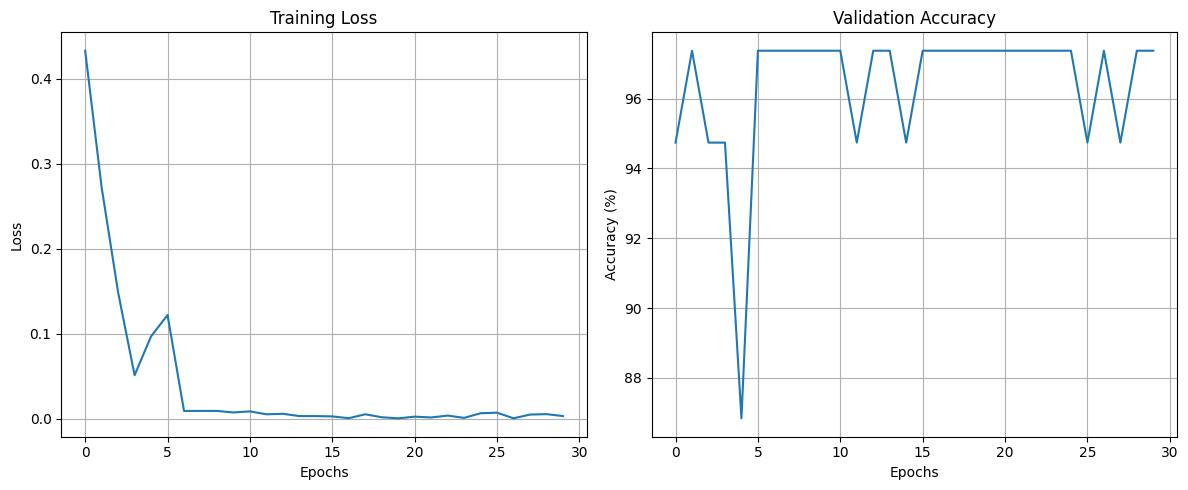
\includegraphics[width=\textwidth]{images/appendix/modelgraph/vgg/vgg.png}
        \caption{Training and validation loss across epochs}
        \label{fig:vgg_training}
    \end{subfigure}
    \hfill
    \begin{subfigure}[b]{0.48\textwidth}
        \centering
        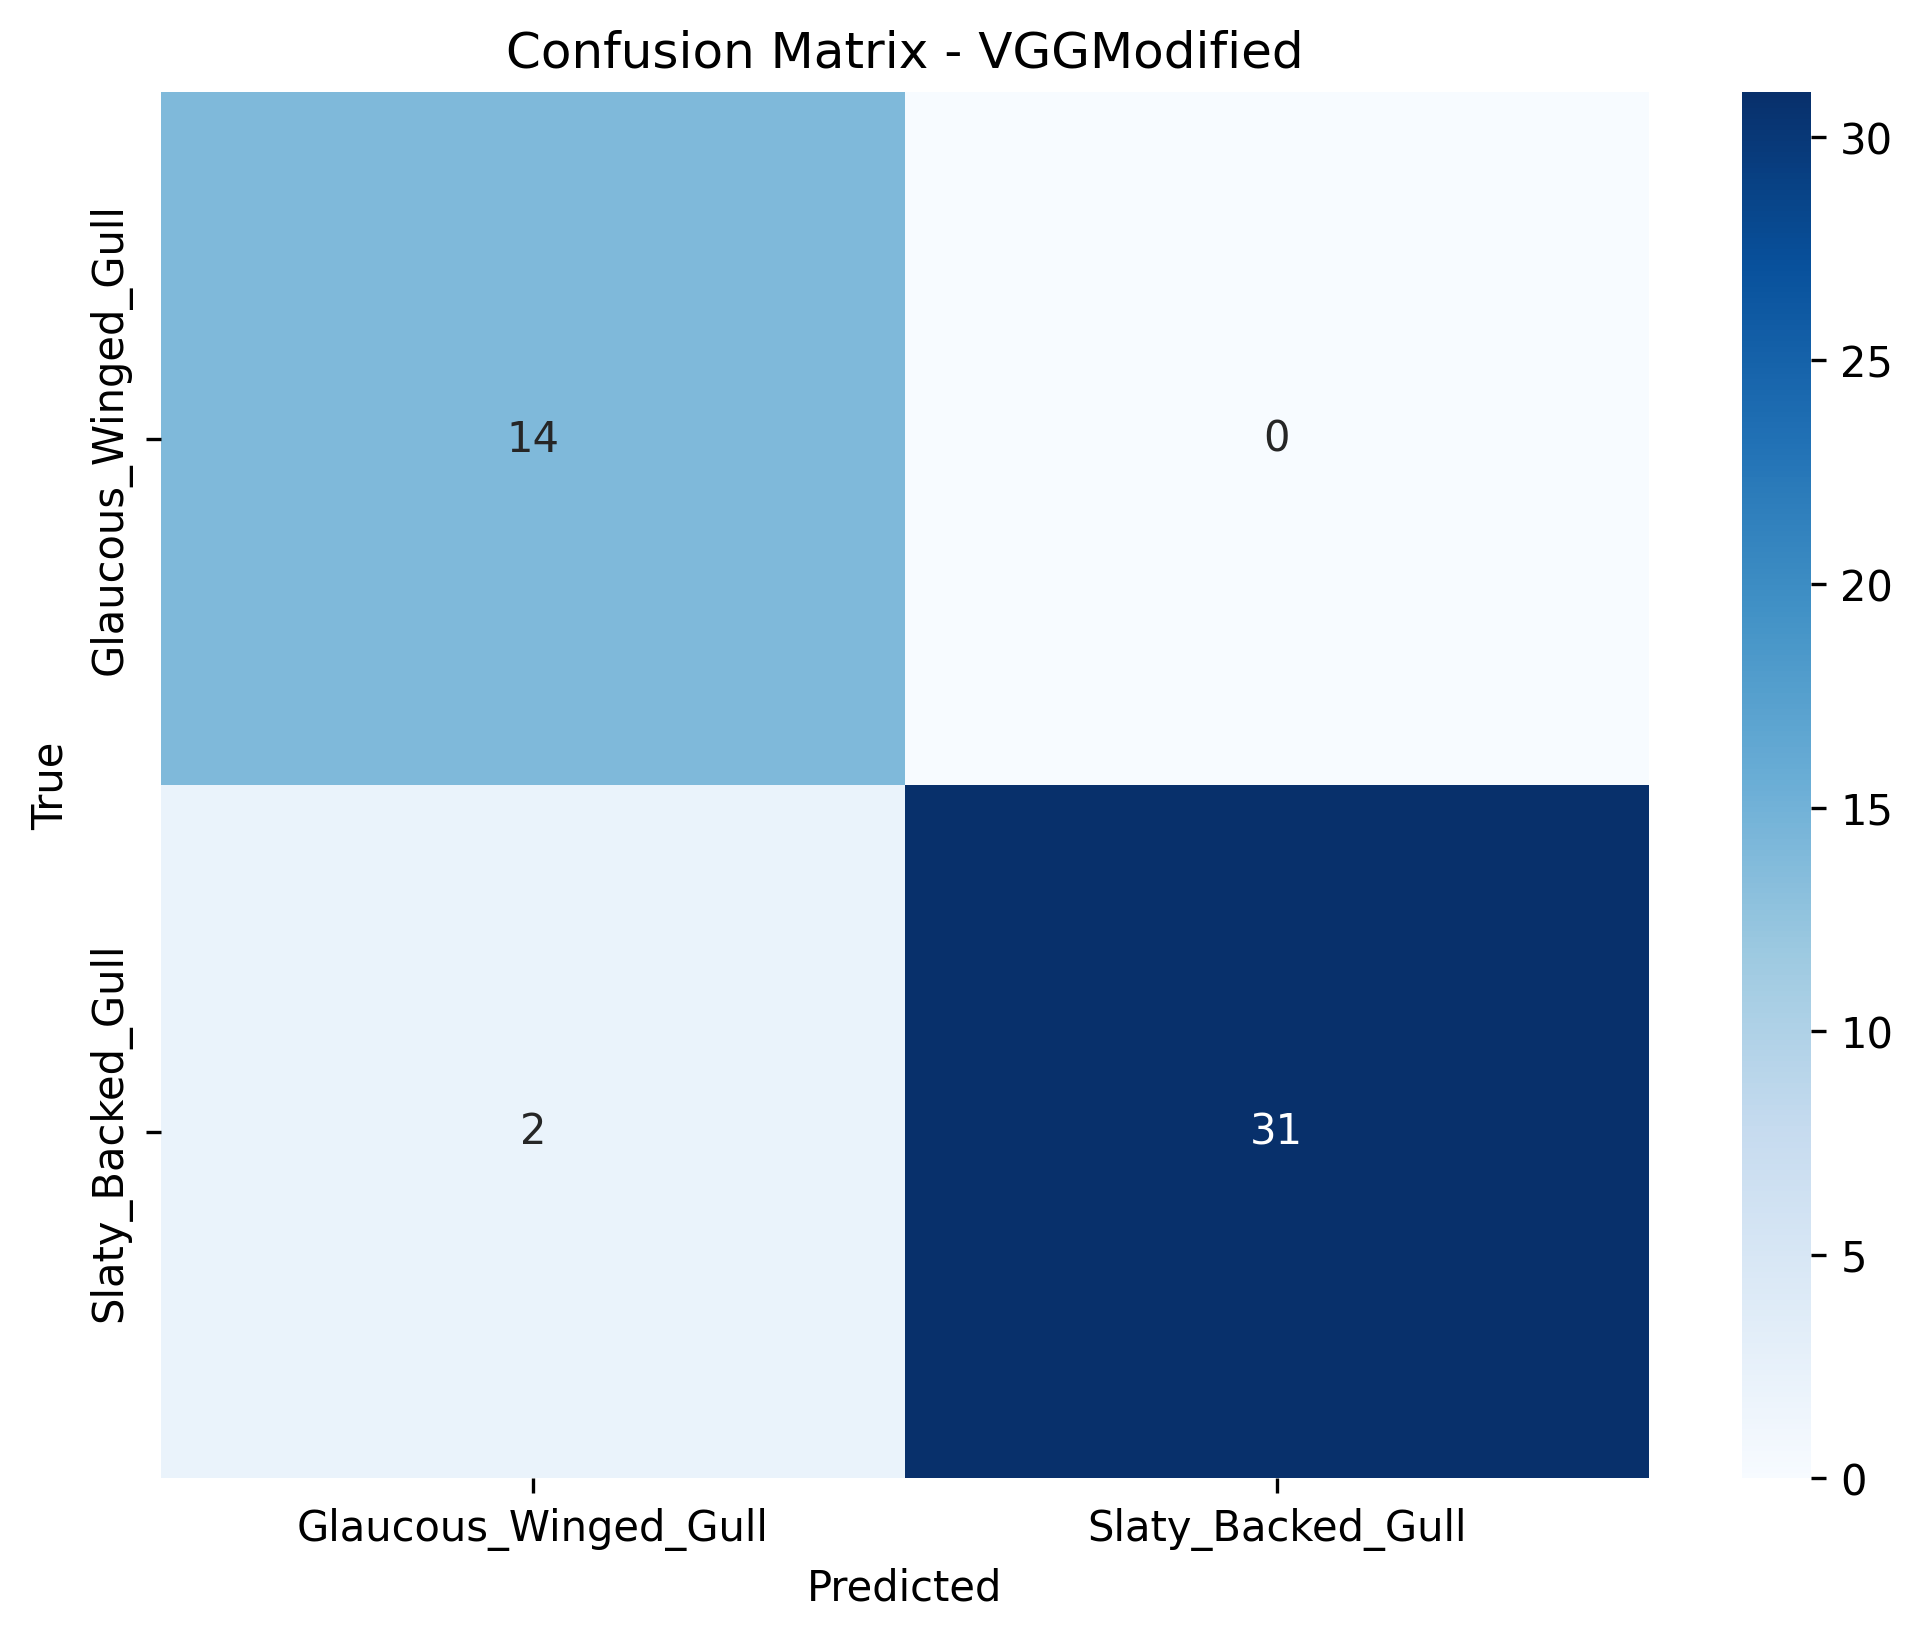
\includegraphics[width=\textwidth]{images/appendix/modelgraph/vgg/vggmodified_confusion_matrix.png}
        \caption{Confusion matrix on test set}
        \label{fig:vgg_confusion}
    \end{subfigure}
    \caption{VGG-16 model performance visualization}
    \label{fig:vgg_performance}
\end{figure}

\subsection{Vision Transformer (ViT)}
\begin{figure}[H]
    \centering
    \begin{subfigure}[b]{0.48\textwidth}
        \centering
        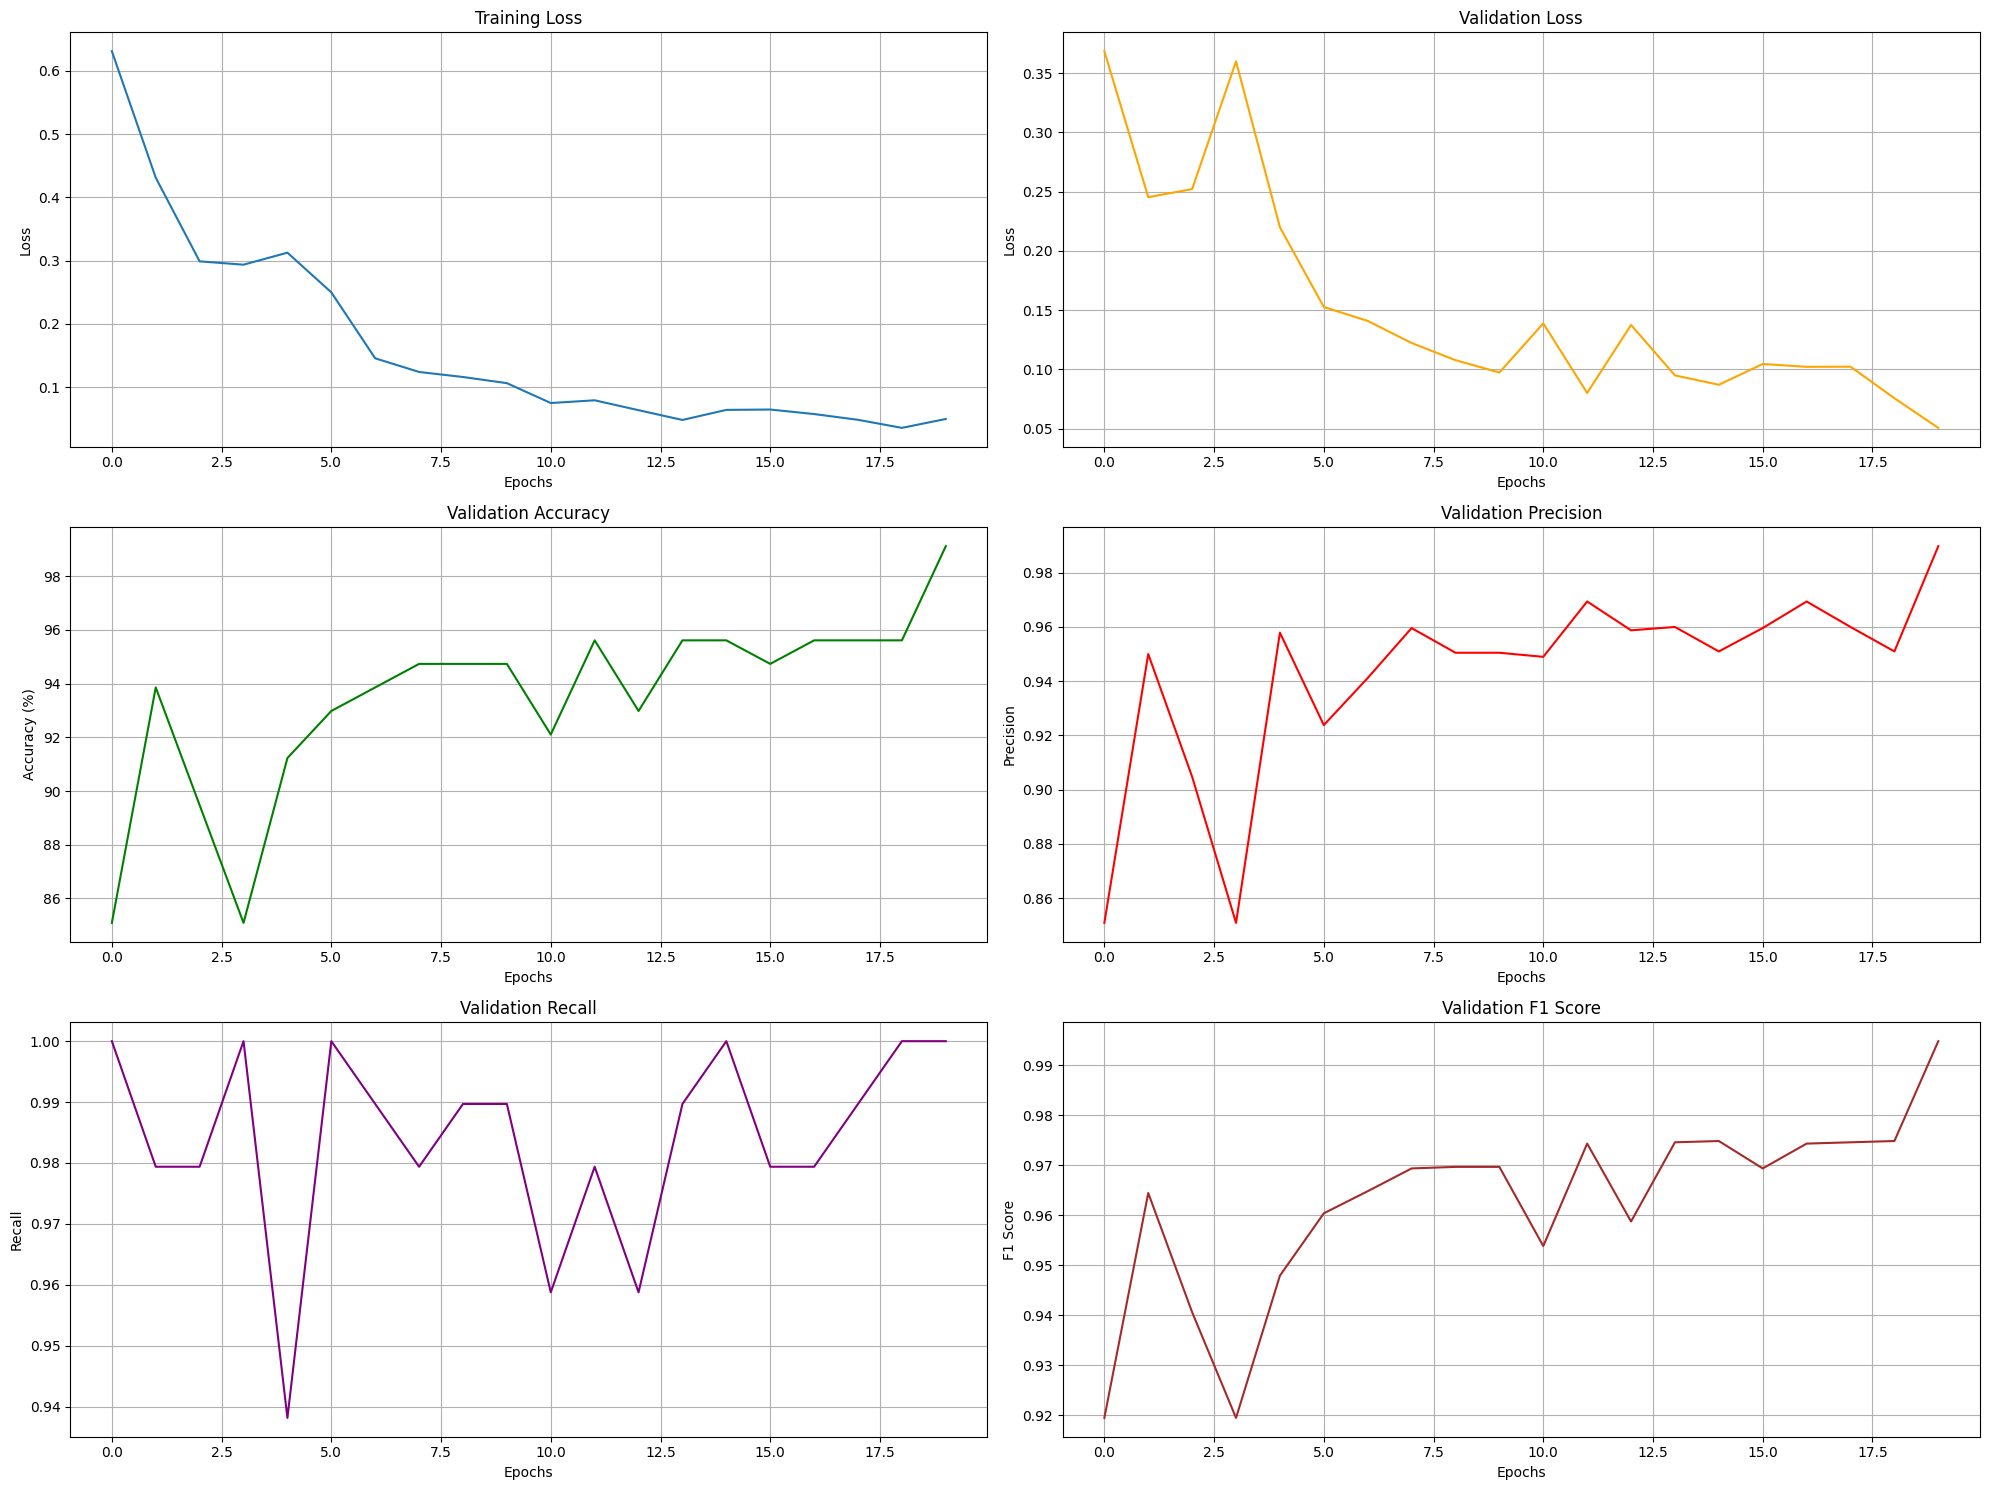
\includegraphics[width=\textwidth]{images/appendix/modelgraph/vit/vit.png}
        \caption{Training and validation loss across epochs}
        \label{fig:vit_training}
    \end{subfigure}
    \hfill
    \begin{subfigure}[b]{0.48\textwidth}
        \centering
        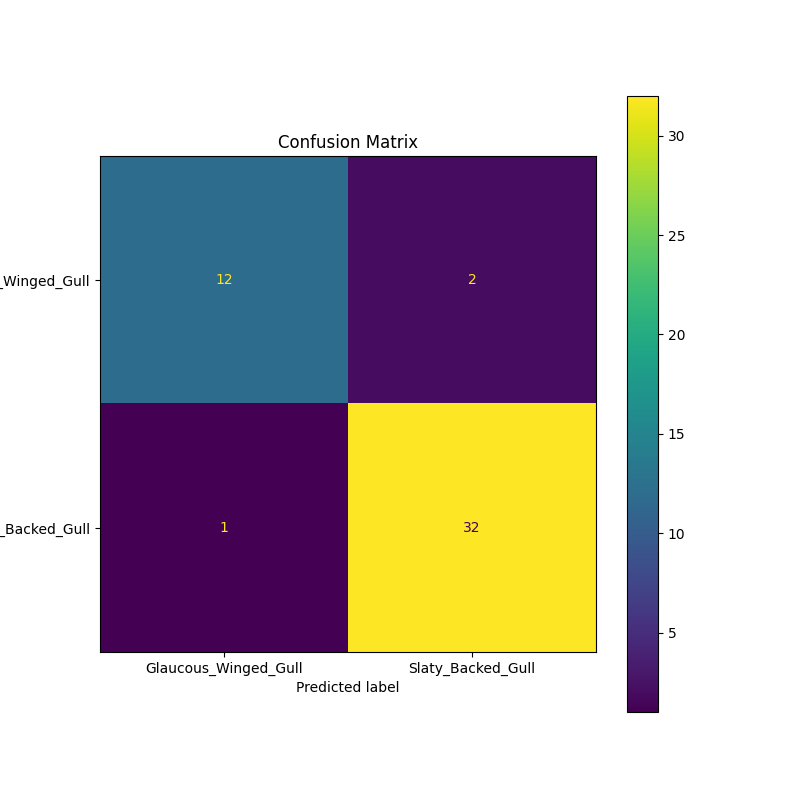
\includegraphics[width=\textwidth]{images/appendix/modelgraph/vit/confusion_matrix.png}
        \caption{Confusion matrix on test set}
        \label{fig:vit_confusion}
    \end{subfigure}
    \caption{Vision Transformer model performance visualization}
    \label{fig:vit_performance}
\end{figure}

\subsection{Inception v3}
\begin{figure}[H]
    \centering
    \begin{subfigure}[b]{0.48\textwidth}
        \centering
        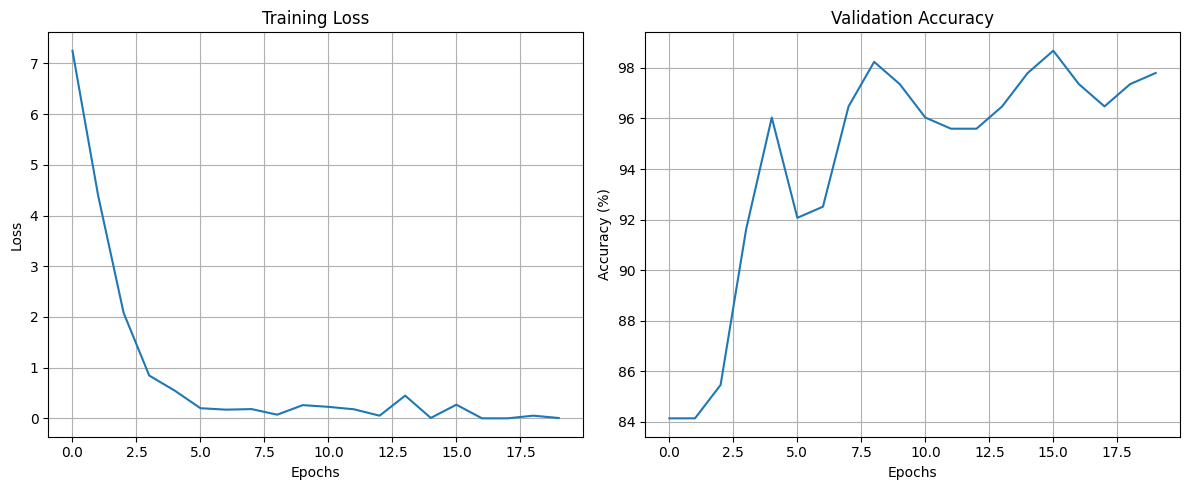
\includegraphics[width=\textwidth]{images/appendix/modelgraph/inception/inception.png}
        \caption{Training and validation loss across epochs}
        \label{fig:inception_training}
    \end{subfigure}
    \hfill
    \begin{subfigure}[b]{0.48\textwidth}
        \centering
        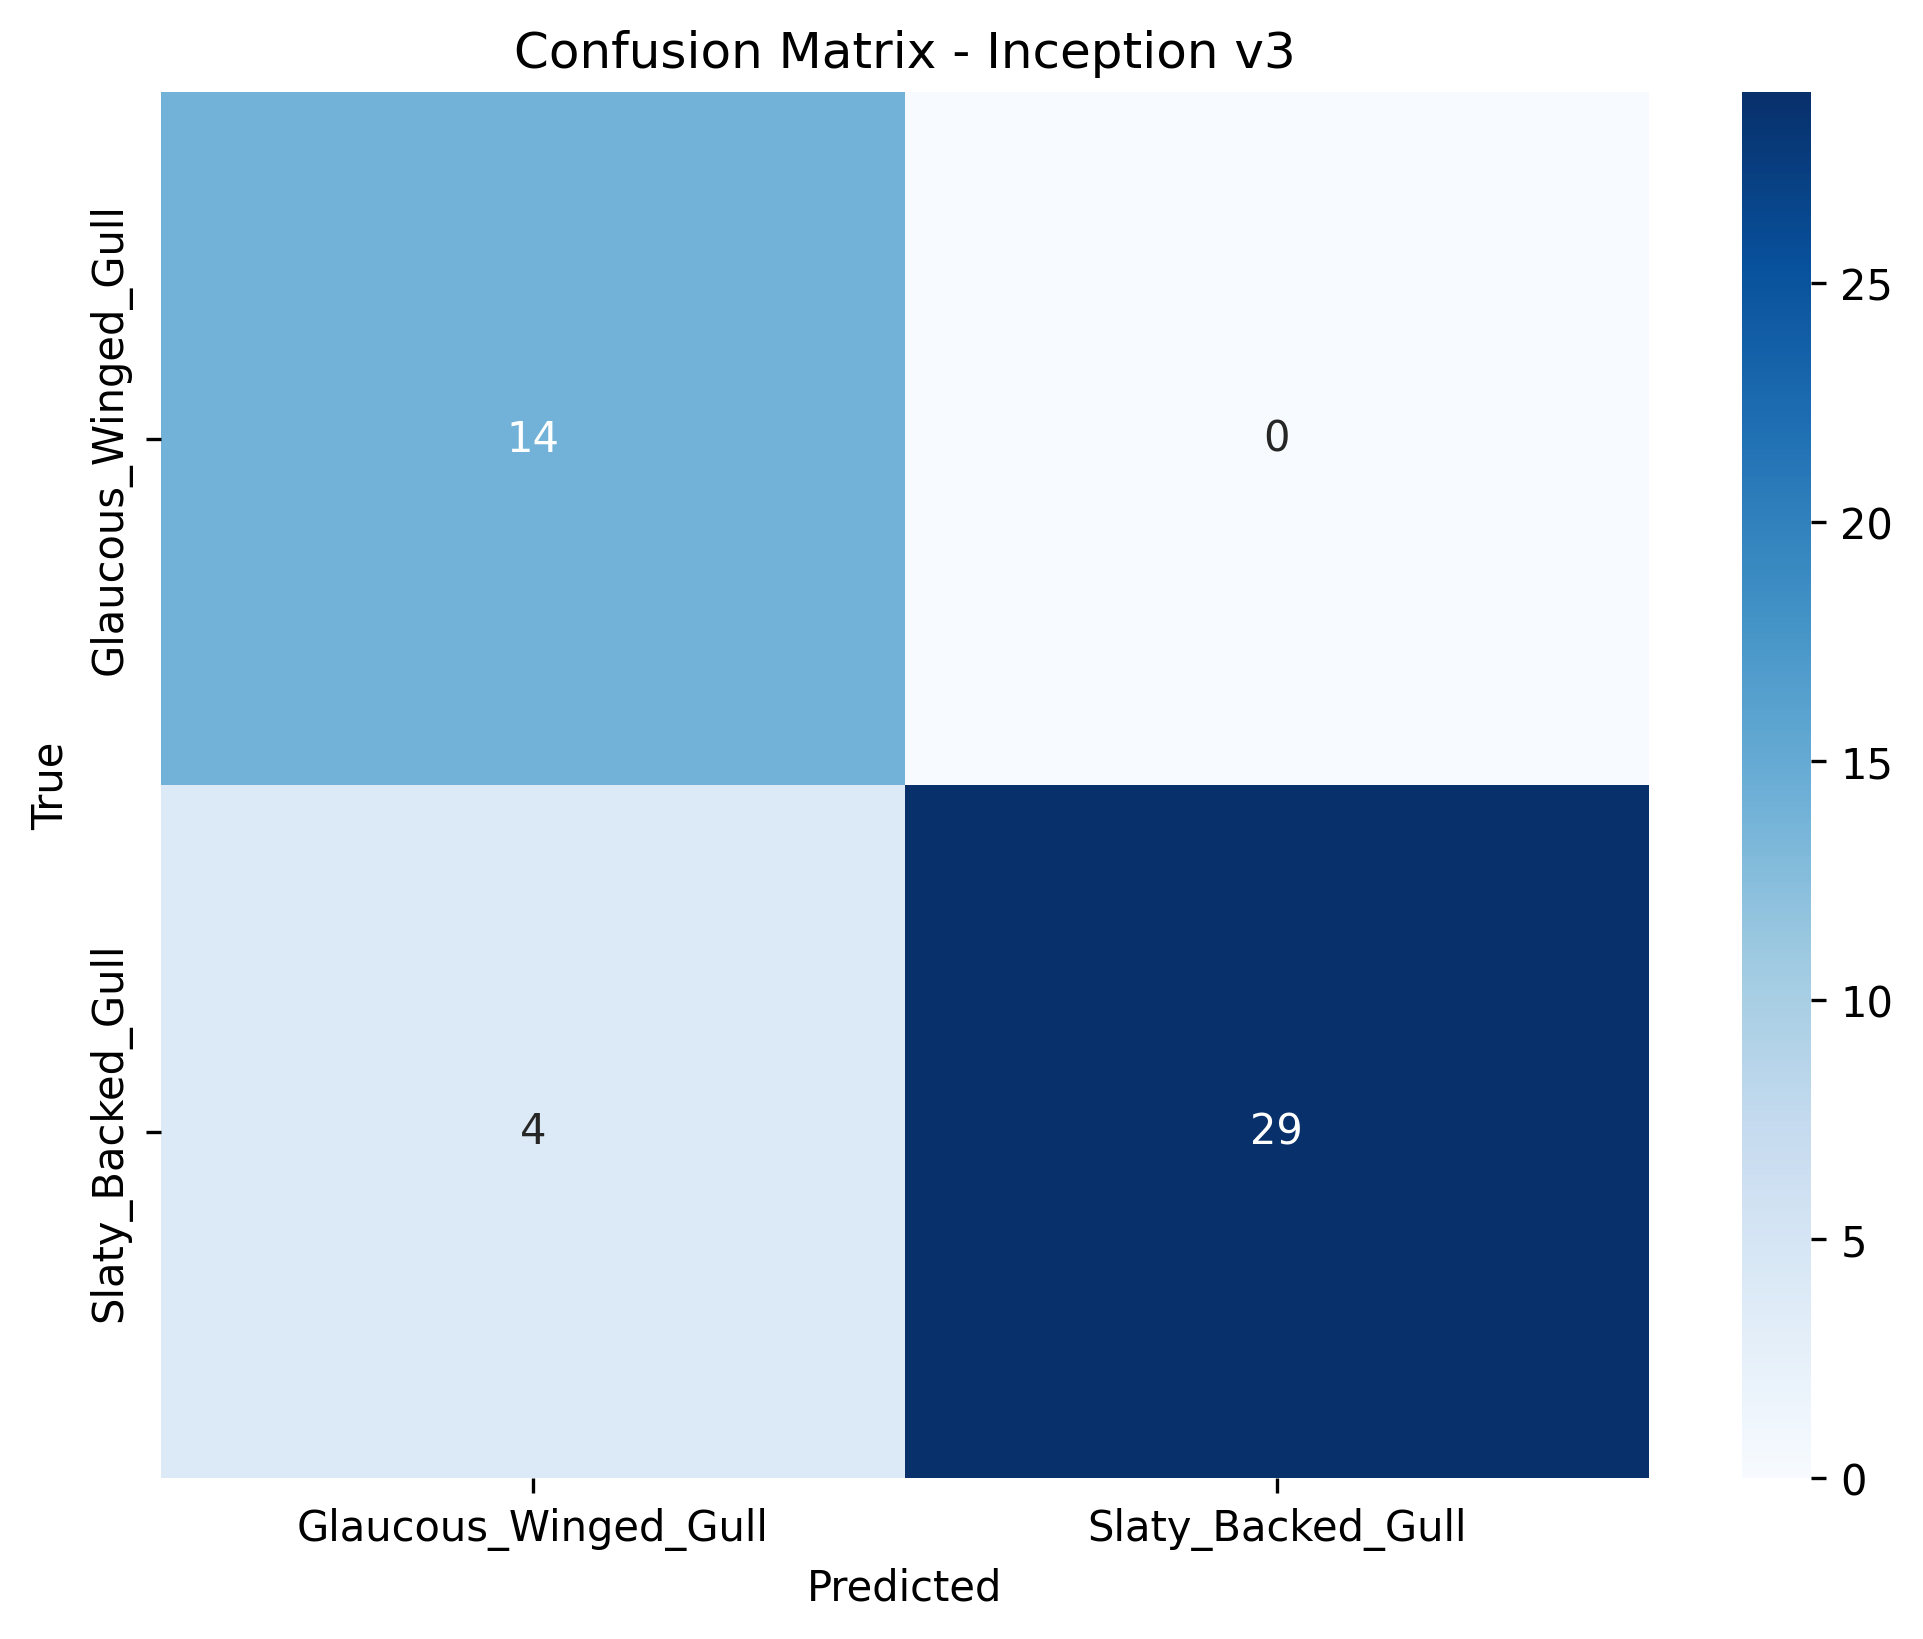
\includegraphics[width=\textwidth]{images/appendix/modelgraph/inception/inception_v3_confusion_matrix.png}
        \caption{Confusion matrix on test set}
        \label{fig:inception_confusion}
    \end{subfigure}
    \caption{Inception v3 model performance visualization}
    \label{fig:inception_performance}
\end{figure}

\subsection{Enhanced Vision Transformer}
\begin{figure}[H]
    \centering
    \begin{subfigure}[b]{0.48\textwidth}
        \centering
        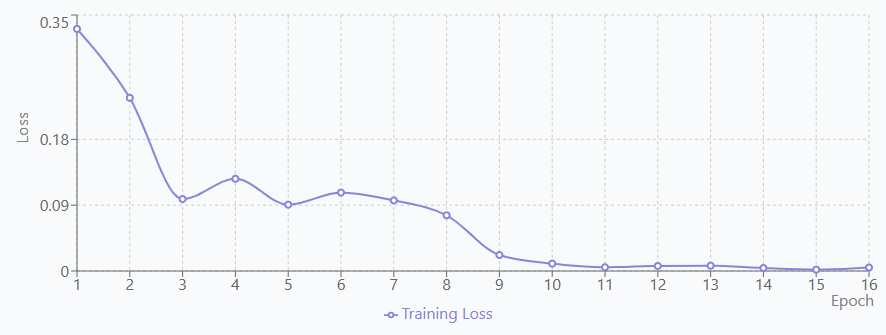
\includegraphics[width=\textwidth]{images/appendix/modelgraph/enhancedvit/enhancedvit.png}
        \caption{Training and validation loss across epochs}
        \label{fig:enhancedvit_training}
    \end{subfigure}
    \hfill
    \begin{subfigure}[b]{0.48\textwidth}
        \centering
        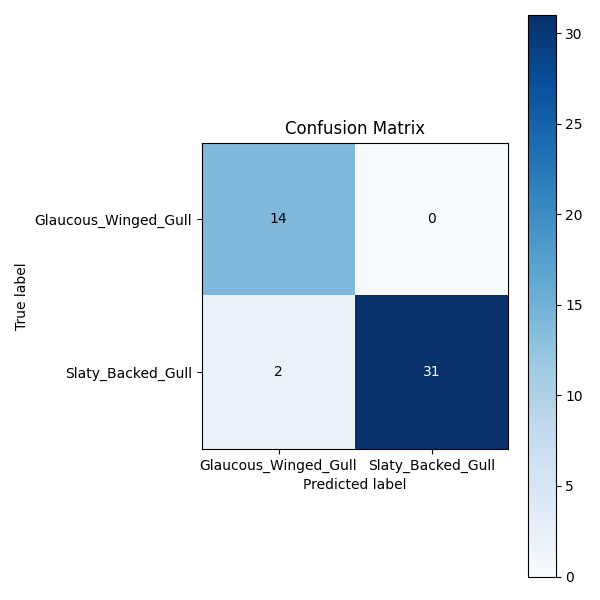
\includegraphics[width=\textwidth]{images/appendix/modelgraph/enhancedvit/confusion_matrix.png}
        \caption{Confusion matrix on test set}
        \label{fig:enhancedvit_confusion}
    \end{subfigure}
    \caption{Enhanced Vision Transformer model performance visualization}
    \label{fig:enhancedvit_performance}
\end{figure}

\subsection{Interpretable Vision Transformer}
\begin{figure}[H]
    \centering
    \begin{subfigure}[b]{0.48\textwidth}
        \centering
        \includegraphics[width=\textwidth]{images/appendix/modelgraph/interpretablevit/interpretablevit.png}
        \caption{Training and validation loss across epochs}
        \label{fig:interpretablevit_training}
    \end{subfigure}
    \hfill
    \begin{subfigure}[b]{0.48\textwidth}
        \centering
        \includegraphics[width=\textwidth]{images/appendix/modelgraph/interpretablevit/confusion_matrix.png}
        \caption{Confusion matrix on test set}
        \label{fig:interpretablevit_confusion}
    \end{subfigure}
    \caption{Interpretable Vision Transformer model performance visualization}
    \label{fig:interpretablevit_performance}
\end{figure}

\subsection{ResNet50}
\begin{figure}[H]
    \centering
    \begin{subfigure}[b]{0.48\textwidth}
        \centering
        \includegraphics[width=\textwidth]{images/appendix/modelgraph/resnet/resnet.png}
        \caption{Training and validation loss across epochs}
        \label{fig:resnet_training}
    \end{subfigure}
    \hfill
    \begin{subfigure}[b]{0.48\textwidth}
        \centering
        \includegraphics[width=\textwidth]{images/appendix/modelgraph/resnet/resnet50_confusion_matrix.png}
        \caption{Confusion matrix on test set}
        \label{fig:resnet_confusion}
    \end{subfigure}
    \caption{ResNet50 model performance visualization}
    \label{fig:resnet_performance}
\end{figure}

\section{Model Interpretability Results}
\label{sec:interpretability}

\subsection{Model Comparison with Grad-CAM results on unseen Test Set}
This section presents the results of Grad-CAM across different models except for ViT which displays the attention rollout results. All the images here were correctly predicted by all the well-performing models below. Each row displays the same image processed by the models that achieved high test and validation accuracy, allowing direct comparison of how each model focuses on different bird features.

\subsubsection{Glaucous Winged Gull Interpretability Results}
\label{subsec:glaucous_interpretability}

% First image - 20241203_010647.jpg
\begin{figure}[H]
    \centering
    \setlength{\tabcolsep}{1pt}
    \begin{tabular}{cccc}
    \textbf{VGG-16} & \textbf{ViT} & \textbf{Inception v3} & \textbf{ResNet50} \\
    
    \includegraphics[width=0.22\textwidth]{images/appendix/modelgraph/vgg/correct/Glaucous_Winged_Gull/20241203_010647.jpg} &
    \includegraphics[width=0.22\textwidth]{images/appendix/modelgraph/vit/correct/Glaucous_Winged_Gull/20241203_010647.jpg} &
    \includegraphics[width=0.22\textwidth]{images/appendix/modelgraph/inception/correct/Glaucous_Winged_Gull/20241203_010647.jpg} &
    \includegraphics[width=0.22\textwidth]{images/appendix/modelgraph/resnet/correct/Glaucous_Winged_Gull/20241203_010647.jpg} \\
    \end{tabular}

    \label{fig:interpretability_glaucous_1}
\end{figure}

% Second image - 20241204_140935.jpg
\begin{figure}[H]
    \centering
    \setlength{\tabcolsep}{1pt}
    \begin{tabular}{cccc}
    \textbf{VGG-16} & \textbf{ViT} & \textbf{Inception v3} & \textbf{ResNet50} \\
    
    \includegraphics[width=0.22\textwidth]{images/appendix/modelgraph/vgg/correct/Glaucous_Winged_Gull/20241204_140935.jpg} &
    \includegraphics[width=0.22\textwidth]{images/appendix/modelgraph/vit/correct/Glaucous_Winged_Gull/20241204_140935.jpg} &
    \includegraphics[width=0.22\textwidth]{images/appendix/modelgraph/inception/correct/Glaucous_Winged_Gull/20241204_140935.jpg} &
    \includegraphics[width=0.22\textwidth]{images/appendix/modelgraph/resnet/correct/Glaucous_Winged_Gull/20241204_140935.jpg} \\
    \end{tabular}
 
    \label{fig:interpretability_glaucous_2}
\end{figure}

% Third image - 20241204_170956.jpg
\begin{figure}[H]
    \centering
    \setlength{\tabcolsep}{1pt}
    \begin{tabular}{cccc}
    \textbf{VGG-16} & \textbf{ViT} & \textbf{Inception v3} & \textbf{ResNet50} \\
    
    \includegraphics[width=0.22\textwidth]{images/appendix/modelgraph/vgg/correct/Glaucous_Winged_Gull/20241204_170956.jpg} &
    \includegraphics[width=0.22\textwidth]{images/appendix/modelgraph/vit/correct/Glaucous_Winged_Gull/20241204_170956.jpg} &
    \includegraphics[width=0.22\textwidth]{images/appendix/modelgraph/inception/correct/Glaucous_Winged_Gull/20241204_170956.jpg} &
    \includegraphics[width=0.22\textwidth]{images/appendix/modelgraph/resnet/correct/Glaucous_Winged_Gull/20241204_170956.jpg} \\
    \end{tabular}

    \label{fig:interpretability_glaucous_3}
\end{figure}

% Fourth image - 20241204_171004.jpg
\begin{figure}[H]
    \centering
    \setlength{\tabcolsep}{1pt}
    \begin{tabular}{cccc}
    \textbf{VGG-16} & \textbf{ViT} & \textbf{Inception v3} & \textbf{ResNet50} \\
    
    \includegraphics[width=0.22\textwidth]{images/appendix/modelgraph/vgg/correct/Glaucous_Winged_Gull/20241204_171004.jpg} &
    \includegraphics[width=0.22\textwidth]{images/appendix/modelgraph/vit/correct/Glaucous_Winged_Gull/20241204_171004.jpg} &
    \includegraphics[width=0.22\textwidth]{images/appendix/modelgraph/inception/correct/Glaucous_Winged_Gull/20241204_171004.jpg} &
    \includegraphics[width=0.22\textwidth]{images/appendix/modelgraph/resnet/correct/Glaucous_Winged_Gull/20241204_171004.jpg} \\
    \end{tabular}

    \label{fig:interpretability_glaucous_4}
\end{figure}

% Fifth image - 20241204_171110.jpg
\begin{figure}[H]
    \centering
    \setlength{\tabcolsep}{1pt}
    \begin{tabular}{cccc}
    \textbf{VGG-16} & \textbf{ViT} & \textbf{Inception v3} & \textbf{ResNet50} \\
    
    \includegraphics[width=0.22\textwidth]{images/appendix/modelgraph/vgg/correct/Glaucous_Winged_Gull/20241204_171110.jpg} &
    \includegraphics[width=0.22\textwidth]{images/appendix/modelgraph/vit/correct/Glaucous_Winged_Gull/20241204_171110.jpg} &
    \includegraphics[width=0.22\textwidth]{images/appendix/modelgraph/inception/correct/Glaucous_Winged_Gull/20241204_171110.jpg} &
    \includegraphics[width=0.22\textwidth]{images/appendix/modelgraph/resnet/correct/Glaucous_Winged_Gull/20241204_171110.jpg} \\
    \end{tabular}
 
    \label{fig:interpretability_glaucous_5}
\end{figure}

% Sixth image - 3O4A8774 - Version 2.JPG
\begin{figure}[H]
    \centering
    \setlength{\tabcolsep}{1pt}
    \begin{tabular}{cccc}
    \textbf{VGG-16} & \textbf{ViT} & \textbf{Inception v3} & \textbf{ResNet50} \\
    
    \includegraphics[width=0.22\textwidth]{images/appendix/modelgraph/vgg/correct/Glaucous_Winged_Gull/3O4A8774 - Version 2.JPG} &
    \includegraphics[width=0.22\textwidth]{images/appendix/modelgraph/vit/correct/Glaucous_Winged_Gull/3O4A8774 - Version 2.JPG} &
    \includegraphics[width=0.22\textwidth]{images/appendix/modelgraph/inception/correct/Glaucous_Winged_Gull/3O4A8774 - Version 2.JPG} &
    \includegraphics[width=0.22\textwidth]{images/appendix/modelgraph/resnet/correct/Glaucous_Winged_Gull/3O4A8774 - Version 2.JPG} \\
    \end{tabular}

    \label{fig:interpretability_glaucous_6}
\end{figure}

\clearpage
\subsubsection{Slaty Backed Gull Interpretability Results}
\label{subsec:slaty_interpretability}

% First image - 011sm.jpg
\begin{figure}[H]
    \centering
    \setlength{\tabcolsep}{1pt}
    \begin{tabular}{cccc}
    \textbf{VGG-16} & \textbf{ViT} & \textbf{Inception v3} & \textbf{ResNet50} \\
    
    \includegraphics[width=0.22\textwidth]{images/appendix/modelgraph/vgg/correct/Slaty_Backed_Gull/011sm.jpg} &
    \includegraphics[width=0.22\textwidth]{images/appendix/modelgraph/vit/correct/Slaty_Backed_Gull/011sm.jpg} &
    \includegraphics[width=0.22\textwidth]{images/appendix/modelgraph/inception/correct/Slaty_Backed_Gull/011sm.jpg} &
    \includegraphics[width=0.22\textwidth]{images/appendix/modelgraph/resnet/correct/Slaty_Backed_Gull/011sm.jpg} \\
    \end{tabular}

    \label{fig:interpretability_slaty_1}
\end{figure}

% Second image - 20241204_141506.jpg
\begin{figure}[H]
    \centering
    \setlength{\tabcolsep}{1pt}
    \begin{tabular}{cccc}
    \textbf{VGG-16} & \textbf{ViT} & \textbf{Inception v3} & \textbf{ResNet50} \\
    
    \includegraphics[width=0.22\textwidth]{images/appendix/modelgraph/vgg/correct/Slaty_Backed_Gull/20241204_141506.jpg} &
    \includegraphics[width=0.22\textwidth]{images/appendix/modelgraph/vit/correct/Slaty_Backed_Gull/20241204_141506.jpg} &
    \includegraphics[width=0.22\textwidth]{images/appendix/modelgraph/inception/correct/Slaty_Backed_Gull/20241204_141506.jpg} &
    \includegraphics[width=0.22\textwidth]{images/appendix/modelgraph/resnet/correct/Slaty_Backed_Gull/20241204_141506.jpg} \\
    \end{tabular}

    \label{fig:interpretability_slaty_2}
\end{figure}

% Third image - 20241204_170322.jpg
\begin{figure}[H]
    \centering
    \setlength{\tabcolsep}{1pt}
    \begin{tabular}{cccc}
    \textbf{VGG-16} & \textbf{ViT} & \textbf{Inception v3} & \textbf{ResNet50} \\
    
    \includegraphics[width=0.22\textwidth]{images/appendix/modelgraph/vgg/correct/Slaty_Backed_Gull/20241204_170322.jpg} &
    \includegraphics[width=0.22\textwidth]{images/appendix/modelgraph/vit/correct/Slaty_Backed_Gull/20241204_170322.jpg} &
    \includegraphics[width=0.22\textwidth]{images/appendix/modelgraph/inception/correct/Slaty_Backed_Gull/20241204_170322.jpg} &
    \includegraphics[width=0.22\textwidth]{images/appendix/modelgraph/resnet/correct/Slaty_Backed_Gull/20241204_170322.jpg} \\
    \end{tabular}

    \label{fig:interpretability_slaty_3}
\end{figure}

% Fourth image - 20241204_170332.jpg
\begin{figure}[H]
    \centering
    \setlength{\tabcolsep}{1pt}
    \begin{tabular}{cccc}
    \textbf{VGG-16} & \textbf{ViT} & \textbf{Inception v3} & \textbf{ResNet50} \\
    
    \includegraphics[width=0.22\textwidth]{images/appendix/modelgraph/vgg/correct/Slaty_Backed_Gull/20241204_170332.jpg} &
    \includegraphics[width=0.22\textwidth]{images/appendix/modelgraph/vit/correct/Slaty_Backed_Gull/20241204_170332.jpg} &
    \includegraphics[width=0.22\textwidth]{images/appendix/modelgraph/inception/correct/Slaty_Backed_Gull/20241204_170332.jpg} &
    \includegraphics[width=0.22\textwidth]{images/appendix/modelgraph/resnet/correct/Slaty_Backed_Gull/20241204_170332.jpg} \\
    \end{tabular}

    \label{fig:interpretability_slaty_4}
\end{figure}

% Fifth image - 480 (1).jpeg
\begin{figure}[H]
    \centering
    \setlength{\tabcolsep}{1pt}
    \begin{tabular}{cccc}
    \textbf{VGG-16} & \textbf{ViT} & \textbf{Inception v3} & \textbf{ResNet50} \\
    
    \includegraphics[width=0.22\textwidth]{images/appendix/modelgraph/vgg/correct/Slaty_Backed_Gull/480 (1).jpeg} &
    \includegraphics[width=0.22\textwidth]{images/appendix/modelgraph/vit/correct/Slaty_Backed_Gull/480 (1).jpeg} &
    \includegraphics[width=0.22\textwidth]{images/appendix/modelgraph/inception/correct/Slaty_Backed_Gull/480 (1).jpeg} &
    \includegraphics[width=0.22\textwidth]{images/appendix/modelgraph/resnet/correct/Slaty_Backed_Gull/480 (1).jpeg} \\
    \end{tabular}

    \label{fig:interpretability_slaty_5}
\end{figure}

% Sixth image - 480 (14).jpeg
\begin{figure}[H]
    \centering
    \setlength{\tabcolsep}{1pt}
    \begin{tabular}{cccc}
    \textbf{VGG-16} & \textbf{ViT} & \textbf{Inception v3} & \textbf{ResNet50} \\
    
    \includegraphics[width=0.22\textwidth]{images/appendix/modelgraph/vgg/correct/Slaty_Backed_Gull/480 (14).jpeg} &
    \includegraphics[width=0.22\textwidth]{images/appendix/modelgraph/vit/correct/Slaty_Backed_Gull/480 (14).jpeg} &
    \includegraphics[width=0.22\textwidth]{images/appendix/modelgraph/inception/correct/Slaty_Backed_Gull/480 (14).jpeg} &
    \includegraphics[width=0.22\textwidth]{images/appendix/modelgraph/resnet/correct/Slaty_Backed_Gull/480 (14).jpeg} \\
    \end{tabular}

    \label{fig:interpretability_slaty_6}
\end{figure}

% Seventh image - 480 (19).jpeg
\begin{figure}[H]
    \centering
    \setlength{\tabcolsep}{1pt}
    \begin{tabular}{cccc}
    \textbf{VGG-16} & \textbf{ViT} & \textbf{Inception v3} & \textbf{ResNet50} \\
    
    \includegraphics[width=0.22\textwidth]{images/appendix/modelgraph/vgg/correct/Slaty_Backed_Gull/480 (19).jpeg} &
    \includegraphics[width=0.22\textwidth]{images/appendix/modelgraph/vit/correct/Slaty_Backed_Gull/480 (19).jpeg} &
    \includegraphics[width=0.22\textwidth]{images/appendix/modelgraph/inception/correct/Slaty_Backed_Gull/480 (19).jpeg} &
    \includegraphics[width=0.22\textwidth]{images/appendix/modelgraph/resnet/correct/Slaty_Backed_Gull/480 (19).jpeg} \\
    \end{tabular}

    \label{fig:interpretability_slaty_7}
\end{figure}

% Eighth image - 480 (21).jpeg
\begin{figure}[H]
    \centering
    \setlength{\tabcolsep}{1pt}
    \begin{tabular}{cccc}
    \textbf{VGG-16} & \textbf{ViT} & \textbf{Inception v3} & \textbf{ResNet50} \\
    
    \includegraphics[width=0.22\textwidth]{images/appendix/modelgraph/vgg/correct/Slaty_Backed_Gull/480 (21).jpeg} &
    \includegraphics[width=0.22\textwidth]{images/appendix/modelgraph/vit/correct/Slaty_Backed_Gull/480 (21).jpeg} &
    \includegraphics[width=0.22\textwidth]{images/appendix/modelgraph/inception/correct/Slaty_Backed_Gull/480 (21).jpeg} &
    \includegraphics[width=0.22\textwidth]{images/appendix/modelgraph/resnet/correct/Slaty_Backed_Gull/480 (21).jpeg} \\
    \end{tabular}

    \label{fig:interpretability_slaty_8}
\end{figure}

% Ninth image - 480 (3).jpeg
\begin{figure}[H]
    \centering
    \setlength{\tabcolsep}{1pt}
    \begin{tabular}{cccc}
    \textbf{VGG-16} & \textbf{ViT} & \textbf{Inception v3} & \textbf{ResNet50} \\
    
    \includegraphics[width=0.22\textwidth]{images/appendix/modelgraph/vgg/correct/Slaty_Backed_Gull/480 (3).jpeg} &
    \includegraphics[width=0.22\textwidth]{images/appendix/modelgraph/vit/correct/Slaty_Backed_Gull/480 (3).jpeg} &
    \includegraphics[width=0.22\textwidth]{images/appendix/modelgraph/inception/correct/Slaty_Backed_Gull/480 (3).jpeg} &
    \includegraphics[width=0.22\textwidth]{images/appendix/modelgraph/resnet/correct/Slaty_Backed_Gull/480 (3).jpeg} \\
    \end{tabular}
 
    \label{fig:interpretability_slaty_9}
\end{figure}

% Tenth image - 480 (45).jpeg
\begin{figure}[H]
    \centering
    \setlength{\tabcolsep}{1pt}
    \begin{tabular}{cccc}
    \textbf{VGG-16} & \textbf{ViT} & \textbf{Inception v3} & \textbf{ResNet50} \\
    
    \includegraphics[width=0.22\textwidth]{images/appendix/modelgraph/vgg/correct/Slaty_Backed_Gull/480 (45).jpeg} &
    \includegraphics[width=0.22\textwidth]{images/appendix/modelgraph/vit/correct/Slaty_Backed_Gull/480 (45).jpeg} &
    \includegraphics[width=0.22\textwidth]{images/appendix/modelgraph/inception/correct/Slaty_Backed_Gull/480 (45).jpeg} &
    \includegraphics[width=0.22\textwidth]{images/appendix/modelgraph/resnet/correct/Slaty_Backed_Gull/480 (45).jpeg} \\
    \end{tabular}

    \label{fig:interpretability_slaty_10}
\end{figure}


\subsection{InterpretableViT Interpretability Results}

% vitinterpretablegrad images: 2 columns, no captions
\begin{figure}[H]
    \centering
    \begin{subfigure}{0.45\textwidth}
        \includegraphics[width=\linewidth]{images/appendix/vitinterpretablegrad/gradcam_002.png}
    \end{subfigure}
    \begin{subfigure}{0.45\textwidth}
        \includegraphics[width=\linewidth]{images/appendix/vitinterpretablegrad/gradcam_012.png}
    \end{subfigure}
    \vskip\baselineskip
    \begin{subfigure}{0.45\textwidth}
        \includegraphics[width=\linewidth]{images/appendix/vitinterpretablegrad/gradcam_098.png}
    \end{subfigure}
    \begin{subfigure}{0.45\textwidth}
        \includegraphics[width=\linewidth]{images/appendix/vitinterpretablegrad/gradcam_100.png}
    \end{subfigure}
\end{figure}

\subsection{EnhancedViT Interpretability Results}
% vitenhancedcombined images: 1 per row, no captions
\begin{figure}[H]
    \centering
    \includegraphics[width=0.7\textwidth]{images/appendix/vitenhancedcombined/003_combined.png}\\[1ex]
    \includegraphics[width=0.7\textwidth]{images/appendix/vitenhancedcombined/004_combined.png}\\[1ex]
    \includegraphics[width=0.7\textwidth]{images/appendix/vitenhancedcombined/005_combined.png}\\[1ex]
    \includegraphics[width=0.7\textwidth]{images/appendix/vitenhancedcombined/016_combined.png}\\[1ex]
    \includegraphics[width=0.7\textwidth]{images/appendix/vitenhancedcombined/017_combined.png}\\[1ex]
    \includegraphics[width=0.7\textwidth]{images/appendix/vitenhancedcombined/070_combined.png}
\end{figure}

\subsection{Saliency Map Results of ViT model}
% vitsaliency images: 2 columns, no captions
\begin{figure}[H]
    \centering
    \begin{subfigure}{0.45\textwidth}
        \includegraphics[width=\linewidth]{images/appendix/vitsaliency/saliency_007.jpg}
    \end{subfigure}
    \begin{subfigure}{0.45\textwidth}
        \includegraphics[width=\linewidth]{images/appendix/vitsaliency/saliency_480 (29).jpeg}
    \end{subfigure}
    \vskip\baselineskip
    \begin{subfigure}{0.45\textwidth}
        \includegraphics[width=\linewidth]{images/appendix/vitsaliency/saliency_480 (33).jpeg}
    \end{subfigure}
\end{figure}

\subsection{Feature Ablation Result of ViT model}
\begin{figure}[H]
    \centering
    \includegraphics[width=0.8\textwidth]{images/appendix/ablationvit.png}
    \caption{Ablation study for ViT}
    \label{fig:ablationvit}
\end{figure}

\section{Results of different Interpretability techniques of VGG Model}

\begin{figure}[H]
    \centering
    \includegraphics[width=0.9\textwidth]{images/appendix/vggcombined/download.png}
\end{figure}

\begin{figure}[H]
    \centering
    \includegraphics[width=0.9\textwidth]{images/appendix/vggcombined/download12.png}
\end{figure}

\begin{figure}[H]
    \centering
    \includegraphics[width=0.9\textwidth]{images/appendix/vggcombined/download (1).png}
\end{figure}

\begin{figure}[H]
    \centering
    \includegraphics[width=0.9\textwidth]{images/appendix/vggcombined/download2.png}
\end{figure}


\begin{figure}[H]
    \centering
    \includegraphics[width=0.9\textwidth]{images/appendix/vggcombined/download (2).png}
\end{figure}

\begin{figure}[H]
    \centering
    \includegraphics[width=0.9\textwidth]{images/appendix/vggcombined/download1.png}
\end{figure}


\begin{figure}[H]
    \centering
    \includegraphics[width=0.9\textwidth]{images/appendix/vggcombined/download (11).png}
\end{figure}

\begin{figure}[H]
    \centering
    \includegraphics[width=0.9\textwidth]{images/appendix/vggcombined/download11.png}
\end{figure}


\subsection{Saliency Map Results of VGG model}
% deepliftvgg images: 2 columns, no captions
\begin{figure}[H]
    \centering
    \begin{subfigure}{0.45\textwidth}
        \includegraphics[width=\linewidth]{images/appendix/deepliftvgg/download (1).png}
    \end{subfigure}
    \begin{subfigure}{0.45\textwidth}
        \includegraphics[width=\linewidth]{images/appendix/deepliftvgg/download (2).png}
    \end{subfigure}
    \vskip\baselineskip
    \begin{subfigure}{0.45\textwidth}
        \includegraphics[width=\linewidth]{images/appendix/deepliftvgg/download (3).png}
    \end{subfigure}
    \begin{subfigure}{0.45\textwidth}
        \includegraphics[width=\linewidth]{images/appendix/deepliftvgg/download.png}
    \end{subfigure}
\end{figure}

% Continue with remaining Slaty Backed Gull images following the same pattern
% 20241204_170322.jpg, 20241204_170332.jpg, 480 (1).jpeg, 480 (14).jpeg, 
% 480 (19).jpeg, 480 (21).jpeg, 480 (3).jpeg, 480 (45).jpeg


% ... (rest of your preamble)

\section{Local Binary Pattern Analysis Results}
\label{sec:lbp_analysis}

This section displays the LBP analysis results for the wing, wingtip, and head regions of the gull images.

\begin{figure}[H]
    \caption{Histograms for number of ones}
    \centering
    \begin{subfigure}[b]{0.32\textwidth}
        \includegraphics[width=\textwidth]{images/appendix/Number_of_Ones_Analysis/default_head_ones_histogram.png}
        \caption{Head region}
        \label{fig:lbp_head}
    \end{subfigure}
    \hfill
    \begin{subfigure}[b]{0.32\textwidth}
        \includegraphics[width=\textwidth]{images/appendix/Number_of_Ones_Analysis/default_wing_ones_histogram.png}
        \caption{Wing region}
        \label{fig:lbp_wing}
    \end{subfigure}
    \hfill
    \begin{subfigure}[b]{0.32\textwidth}
        \includegraphics[width=\textwidth]{images/appendix/Number_of_Ones_Analysis/default_wingtip_ones_histogram.png}
        \caption{Wingtip region}
        \label{fig:lbp_wingtip}
    \end{subfigure}
    \caption{Local Binary Pattern analysis results showing histograms of pattern distributions across different bird regions.}
    \label{fig:lbp_results}
\end{figure}

\begin{figure}[H]
    \caption{Histograms for number of transitions}
    \centering
    \begin{subfigure}[b]{0.32\textwidth}
        \includegraphics[width=\textwidth]{images/appendix/Transitions_Analysis/default_head_transitions_histogram.png}
        \caption{Head region}
        \label{fig:lbp_head}
    \end{subfigure}
    \hfill
    \begin{subfigure}[b]{0.32\textwidth}
        \includegraphics[width=\textwidth]{images/appendix/Transitions_Analysis/default_wing_transitions_histogram.png}
        \caption{Wing region}
        \label{fig:lbp_wing}
    \end{subfigure}
    \hfill
    \begin{subfigure}[b]{0.32\textwidth}
        \includegraphics[width=\textwidth]{images/appendix/Transitions_Analysis/default_wingtip_transitions_histogram.png}
        \caption{Wingtip region}
        \label{fig:lbp_wingtip}
    \end{subfigure}
    \caption{Local Binary Pattern analysis results showing histograms of pattern distributions across different bird regions.}
    \label{fig:lbp_results}
\end{figure}


\subsection{Calculated Texture-based Feature Comparisons on 1s and Transitions Histogram (Rotation Invariant)}
\begin{figure}[H]
    \centering
    \begin{subfigure}[b]{0.48\textwidth}
        \includegraphics[width=\textwidth]{images/appendix/Original/ones_energy_comparison.png}
        \caption{Ones energy comparison}
    \end{subfigure}
    \hfill
    \begin{subfigure}[b]{0.48\textwidth}
        \includegraphics[width=\textwidth]{images/appendix/Original/ones_entropy_comparison.png}
        \caption{Ones entropy comparison}
    \end{subfigure}
    \vspace{0.5cm}
    \begin{subfigure}[b]{0.48\textwidth}
        \includegraphics[width=\textwidth]{images/appendix/Original/mean_ones_comparison.png}
        \caption{Mean ones comparison}
    \end{subfigure}
    \hfill
    \begin{subfigure}[b]{0.48\textwidth}
        \includegraphics[width=\textwidth]{images/appendix/Original/mean_transitions_comparison.png}
        \caption{Mean transitions comparison}
    \end{subfigure}
    \vspace{0.5cm}
    \begin{subfigure}[b]{0.48\textwidth}
        \includegraphics[width=\textwidth]{images/appendix/Original/transitions_energy_comparison.png}
        \caption{Transitions energy comparison}
    \end{subfigure}
    \hfill
    \begin{subfigure}[b]{0.48\textwidth}
        \includegraphics[width=\textwidth]{images/appendix/Original/transitions_entropy_comparison.png}
        \caption{Transitions entropy comparison}
    \end{subfigure}
    \caption{Selected feature comparison results related to "ones" and "transitions" from the original dataset.}
\end{figure}

\section{PCA Plots of 1s and Transitions Histogram}
\begin{figure}[H]
    \centering
    \begin{subfigure}[b]{0.48\textwidth}
        \includegraphics[width=\textwidth]{images/appendix/Original/pca/head_ones_pca_plot.png}
        \caption{Head ones PCA plot}
    \end{subfigure}
    \hfill
    \begin{subfigure}[b]{0.48\textwidth}
        \includegraphics[width=\textwidth]{images/appendix/Original/pca/head_transitions_pca_plot.png}
        \caption{Head transitions PCA plot}
    \end{subfigure}
    \vspace{0.5cm}
    \begin{subfigure}[b]{0.48\textwidth}
        \includegraphics[width=\textwidth]{images/appendix/Original/pca/wing_ones_pca_plot.png}
        \caption{Wing ones PCA plot}
    \end{subfigure}
    \hfill
    \begin{subfigure}[b]{0.48\textwidth}
        \includegraphics[width=\textwidth]{images/appendix/Original/pca/wing_transitions_pca_plot.png}
        \caption{Wing transitions PCA plot}
    \end{subfigure}
    \vspace{0.5cm}
    \begin{subfigure}[b]{0.48\textwidth}
        \includegraphics[width=\textwidth]{images/appendix/Original/pca/wingtip_ones_pca_plot.png}
        \caption{Wingtip ones PCA plot}
    \end{subfigure}
    \hfill
    \begin{subfigure}[b]{0.48\textwidth}
        \includegraphics[width=\textwidth]{images/appendix/Original/pca/wingtip_transitions_pca_plot.png}
        \caption{Wingtip transitions PCA plot}
    \end{subfigure}
    \caption{PCA plots for "ones" and "transitions" features across head, wing, and wingtip regions.}
\end{figure}

\subsection{Calculated Texture-based Feature Comparisons on LBP Histogram (May be Rotation Variant)}
\begin{figure}[htbp]
    \centering
    \begin{subfigure}[b]{0.48\textwidth}
        \includegraphics[width=\textwidth]{images/appendix/Original/energy_comparison.png}
        \caption{Energy comparison}
    \end{subfigure}
    \hfill
    \begin{subfigure}[b]{0.48\textwidth}
        \includegraphics[width=\textwidth]{images/appendix/Original/entropy_comparison.png}
        \caption{Entropy comparison}
    \end{subfigure}
    \vspace{0.5cm}
    \begin{subfigure}[b]{0.48\textwidth}
        \includegraphics[width=\textwidth]{images/appendix/Original/homogeneity_comparison.png}
        \caption{Homogeneity comparison}
    \end{subfigure}
    \hfill
    \begin{subfigure}[b]{0.48\textwidth}
        \includegraphics[width=\textwidth]{images/appendix/Original/transitions_entropy_comparison.png}
        \caption{Transitions entropy comparison}
    \end{subfigure}
    \caption{Selected feature comparison results from the original dataset.}
\end{figure}

\section{Misclassified Points in Clustering Analysis}

This section presents the misclassified points identified by different clustering algorithms. Each plot highlights the data points that were not correctly grouped according to the ground truth.

\begin{figure}[H]
    \centering
    \begin{subfigure}[b]{0.8\textwidth}
        \includegraphics[width=\textwidth]{images/clustering/gmm_misclassifications.png}
        \caption{Misclassified points using the GMM clustering algorithm.}
    \end{subfigure}
    \vspace{0.5cm}
    \begin{subfigure}[b]{0.8\textwidth}
        \includegraphics[width=\textwidth]{images/clustering/hierarchical_misclassifications.png}
        \caption{Misclassified points using the Hierarchical clustering algorithm.}
    \end{subfigure}
    \vspace{0.5cm}
    \begin{subfigure}[b]{0.8\textwidth}
        \includegraphics[width=\textwidth]{images/clustering/kmeans_misclassifications.png}
        \caption{Misclassified points using the K-Means clustering algorithm.}
    \end{subfigure}
    \caption{Misclassified points by different clustering algorithms.}
\end{figure}













% \section{Local Binary Pattern Analysis Results}
% \label{sec:lbp_analysis}

% This section displays the LBP analysis results for the wing, wingtip, and head regions of the gull images.

% \begin{figure}[H]
%     \centering
%     \begin{subfigure}[b]{0.32\textwidth}
%         \centering
%         \includegraphics[width=\textwidth]{images/appendix/Number_of_Ones_Analysis/default_head_ones_histogram.png}
%         \caption{Head region}
%         \label{fig:lbp_head}
%     \end{subfigure}
%     \hfill
%     \begin{subfigure}[b]{0.32\textwidth}
%         \centering
%         \includegraphics[width=\textwidth]{images/appendix/Number_of_Ones_Analysis/default_wing_ones_histogram.png}
%         \caption{Wing region}
%         \label{fig:lbp_wing}
%     \end{subfigure}
%     \hfill
%     \begin{subfigure}[b]{0.32\textwidth}
%         \centering
%         \includegraphics[width=\textwidth]{images/appendix/Number_of_Ones_Analysis/default_wingtip_ones_histogram.png}
%         \caption{Wingtip region}
%         \label{fig:lbp_wingtip}
%     \end{subfigure}
%     \caption{Local Binary Pattern analysis results showing histograms of pattern distributions across different bird regions}
%     \label{fig:lbp_results}
% \end{figure}

% \subsection{Calculated Texture-based Feature Comparisons on 1s and Transitions Histogram (Rotation Invariant)}
% \begin{figure}[H]
%     \centering
%     \begin{subfigure}[b]{0.48\textwidth}
%         \centering
%         \includegraphics[width=\textwidth]{images/appendix/Original/ones_energy_comparison.png}
%         \caption{Ones energy comparison}
%     \end{subfigure}
%     \hfill
%     \begin{subfigure}[b]{0.48\textwidth}
%         \centering
%         \includegraphics[width=\textwidth]{images/appendix/Original/ones_entropy_comparison.png}
%         \caption{Ones entropy comparison}
%     \end{subfigure}
    
%     \hfill
    
%     \begin{subfigure}[t]{0.48\textwidth}
%         \centering
%         \includegraphics[width=\textwidth]{images/appendix/Original/mean_ones_comparison.png}
%         \caption{Mean ones comparison}
%     \end{subfigure}
%     \hfill
%     \begin{subfigure}[t]{0.48\textwidth}
%         \centering
%         \includegraphics[width=\textwidth]{images/appendix/Original/mean_transitions_comparison.png}
%         \caption{Mean transitions comparison}
%     \end{subfigure}
    
%     \vspace{0.5cm}
    
%     \begin{subfigure}[t]{0.48\textwidth}
%         \centering
%         \includegraphics[width=\textwidth]{images/appendix/Original/transitions_energy_comparison.png}
%         \caption{Transitions energy comparison}
%     \end{subfigure}
%     \hfill
%     \begin{subfigure}[t]{0.48\textwidth}
%         \centering
%         \includegraphics[width=\textwidth]{images/appendix/Original/transitions_entropy_comparison.png}
%         \caption{Transitions entropy comparison}
%     \end{subfigure}
    
%     \caption{Selected feature comparison results related to "ones" and "transitions" from the original dataset.}
% \end{figure}

% \section{PCA Plots of 1s and Transitions Histogram}

% \begin{figure}[H]
%     \centering
%     \begin{subfigure}[t]{0.48\textwidth}
%         \centering
%         \includegraphics[width=\textwidth]{images/appendix/Original/pca/head_ones_pca_plot.png}
%         \caption{Head ones PCA plot}
%     \end{subfigure}
%     \hfill
%     \begin{subfigure}[t]{0.48\textwidth}
%         \centering
%         \includegraphics[width=\textwidth]{images/appendix/Original/pca/head_transitions_pca_plot.png}
%         \caption{Head transitions PCA plot}
%     \end{subfigure}
    
%     \vspace{0.5cm}
    
%     \begin{subfigure}[t]{0.48\textwidth}
%         \centering
%         \includegraphics[width=\textwidth]{images/appendix/Original/pca/wing_ones_pca_plot.png}
%         \caption{Wing ones PCA plot}
%     \end{subfigure}
%     \hfill
%     \begin{subfigure}[t]{0.48\textwidth}
%         \centering
%         \includegraphics[width=\textwidth]{images/appendix/Original/pca/wing_transitions_pca_plot.png}
%         \caption{Wing transitions PCA plot}
%     \end{subfigure}
    
%     \vspace{0.5cm}
    
%     \begin{subfigure}[t]{0.48\textwidth}
%         \centering
%         \includegraphics[width=\textwidth]{images/appendix/Original/pca/wingtip_ones_pca_plot.png}
%         \caption{Wingtip ones PCA plot}
%     \end{subfigure}
%     \hfill
%     \begin{subfigure}[t]{0.48\textwidth}
%         \centering
%         \includegraphics[width=\textwidth]{images/appendix/Original/pca/wingtip_transitions_pca_plot.png}
%         \caption{Wingtip transitions PCA plot}
%     \end{subfigure}
    
%     \caption{PCA plots for "ones" and "transitions" features across head, wing, and wingtip regions.}
% \end{figure}

% \subsection{Calculated Texture-based Feature Comparisons on LBP Histogram (May be Rotation Variant)}
% \begin{figure}[H]
%     \centering
%     \begin{subfigure}[t]{0.48\textwidth}
%         \centering
%         \includegraphics[width=\textwidth]{images/appendix/Original/energy_comparison.png}
%         \caption{Energy comparison}
%     \end{subfigure}
%     \hfill
%     \begin{subfigure}[t]{0.48\textwidth}
%         \centering
%         \includegraphics[width=\textwidth]{images/appendix/Original/entropy_comparison.png}
%         \caption{Entropy comparison}
%     \end{subfigure}
    
%     \vspace{0.5cm}
    
%     \begin{subfigure}[t]{0.48\textwidth}
%         \centering
%         \includegraphics[width=\textwidth]{images/appendix/Original/homogeneity_comparison.png}
%         \caption{Homogeneity comparison}
%     \end{subfigure}
%     \hfill
%     \begin{subfigure}[t]{0.48\textwidth}
%         \centering
%         \includegraphics[width=\textwidth]{images/appendix/Original/transitions_entropy_comparison.png}
%         \caption{Transitions entropy comparison}
%     \end{subfigure}
    
%     \caption{Selected feature comparison results from the original dataset.}
% \end{figure}

% \section{Misclassified Points in Clustering Analysis}

% This section presents the misclassified points identified by different clustering algorithms. Each plot highlights the data points that were not correctly grouped according to the ground truth.

% \begin{figure}[H]
%     \centering
%     \includegraphics[width=0.8\textwidth]{images/clustering/gmm_misclassifications.png}
%     \caption{Misclassified points using the GMM clustering algorithm.}
% \end{figure}

% \begin{figure}[H]
%     \centering
%     \includegraphics[width=0.8\textwidth]{images/clustering/hierarchical_misclassifications.png}
%     \caption{Misclassified points using the Hierarchical clustering algorithm.}
% \end{figure}

% \begin{figure}[H]
%     \centering
%     \includegraphics[width=0.8\textwidth]{images/clustering/kmeans_misclassifications.png}
%     \caption{Misclassified points using the K-Means clustering algorithm.}
% \end{figure}

\end{document}